%% For normal draft builds (figs undisplayed hence fast compile)
%\documentclass[hyperpdf,nobind,draft,oneside]{hepthesis}
%\documentclass[hyperpdf,nobind,draft,twoside]{hepthesis}

%% For short draft builds (breaks citations by necessity)
%\documentclass[hyperpdf,nobind,draft,hidefrontback]{hepthesis}

%%For Cambridge soft-bound version
%\documentclass[hyperpdf,bindnopdf]{hepthesis}
%% For Cambridge hard-bound version (must be one-sided)
\documentclass[hyperpdf,oneside]{hepthesis}

%% Load special font packages here if you wish
%\usepackage{lmodern}
\usepackage{mathpazo}
%\usepackage{euler}

%% Put package includes etc. into preamble.tex for convenience
\usepackage{xspace}
\usepackage{tikz}
\usepackage{morefloats,subfig,afterpage}
\usepackage{mathrsfs} % script font
\usepackage{verbatim}
\usepackage[printonlyused]{acronym}
%\usepackage{subfigure}
\usepackage{multirow}
\usepackage{lscape}

% \usepackage{hyperref}    % Hyperlinks in references
% \usepackage[all]{hypcap} % Internal hyperlinks to floats.

%% Using Babel allows other languages to be used and mixed-in easily
%\usepackage[ngerman,english]{babel}
\usepackage[english]{babel}
\selectlanguage{english}

%% Citation system tweaks
\usepackage{cite}
% \let\@OldCite\cite
% \renewcommand{\cite}[1]{\mbox{\!\!\!\@OldCite{#1}}}

%% Maths
% TODO: rework or eliminate maybemath
\usepackage{abmath}
\DeclareRobustCommand{\mymath}[1]{\ensuremath{\maybebmsf{#1}}}
% \DeclareRobustCommand{\parenths}[1]{\mymath{\left({#1}\right)}\xspace}
% \DeclareRobustCommand{\braces}[1]{\mymath{\left\{{#1}\right\}}\xspace}
% \DeclareRobustCommand{\angles}[1]{\mymath{\left\langle{#1}\right\rangle}\xspace}
% \DeclareRobustCommand{\sqbracs}[1]{\mymath{\left[{#1}\right]}\xspace}
% \DeclareRobustCommand{\mods}[1]{\mymath{\left\lvert{#1}\right\rvert}\xspace}
% \DeclareRobustCommand{\modsq}[1]{\mymath{\mods{#1}^2}\xspace}
% \DeclareRobustCommand{\dblmods}[1]{\mymath{\left\lVert{#1}\right\rVert}\xspace}
% \DeclareRobustCommand{\expOf}[1]{\mymath{\exp{\!\parenths{#1}}}\xspace}
% \DeclareRobustCommand{\eexp}[1]{\mymath{e^{#1}}\xspace}
% \DeclareRobustCommand{\plusquad}{\mymath{\oplus}\xspace}
% \DeclareRobustCommand{\logOf}[1]{\mymath{\log\!\parenths{#1}}\xspace}
% \DeclareRobustCommand{\lnOf}[1]{\mymath{\ln\!\parenths{#1}}\xspace}
% \DeclareRobustCommand{\ofOrder}[1]{\mymath{\mathcal{O}\parenths{#1}}\xspace}
% \DeclareRobustCommand{\SOgroup}[1]{\mymath{\mathup{SO}\parenths{#1}}\xspace}
% \DeclareRobustCommand{\SUgroup}[1]{\mymath{\mathup{SU}\parenths{#1}}\xspace}
% \DeclareRobustCommand{\Ugroup}[1]{\mymath{\mathup{U}\parenths{#1}}\xspace}
% \DeclareRobustCommand{\I}[1]{\mymath{\mathrm{i}}\xspace}
% \DeclareRobustCommand{\colvector}[1]{\mymath{\begin{pmatrix}#1\end{pmatrix}}\xspace}
\DeclareRobustCommand{\Rate}{\mymath{\Gamma}\xspace}
\DeclareRobustCommand{\RateOf}[1]{\mymath{\Gamma}\parenths{#1}\xspace}

%% High-energy physics stuff
\usepackage{abhep}
\usepackage{hepnames}
\usepackage{hepunits}

%

\newcommand\rs{\raisebox{1.0ex}[-1.0ex]}
\newcommand{\ra}{\ensuremath{\rightarrow}}
\newcommand{\znunu}{\ensuremath{{\text Z} \ra \nu\bar{\nu}}\xspace}
\newcommand{\zll}{\ensuremath{{\text Z} \ra \ell\ell}\xspace}
\newcommand{\zmumu}{\ensuremath{{\text Z} \ra \mu\mu}\xspace}
\newcommand{\zee}{\ensuremath{{\text Z} \ra ee}\xspace}
\newcommand{\wmunu}{\ensuremath{{\text W} \ra \mu\nu}}
\newcommand{\wtaunu}{\ensuremath{{\text W} \ra \tau\nu}}
\newcommand{\dphi}{\ensuremath{\Delta \phi}}
\newcommand{\dphijj}{\ensuremath{\Delta \phi_{ j1,j2}}}
\newcommand{\Pt}{\ensuremath{{p_{\text T}}}\xspace}
%\newcommand{\pT}{\ensuremath{{p_{\text T}}}\xspace}
\newcommand{\pt}{\ensuremath{{p_{\text T}}}\xspace}
\newcommand{\pts}{\ensuremath{p_{\text T}{\text s}}\xspace}
%\newcommand{\Et}{\ensuremath{{E_{\text T}}}\xspace}
\newcommand{\ptjf}{\ensuremath{p_{\rm T}^{ {\rm j}_1} }}
\newcommand{\ptjs}{\ensuremath{p_{\rm T}^{ {\rm j}_2} }}
\newcommand{\ptjt}{\ensuremath{p_{\rm T}^{ {\rm j}_3} }}
\newcommand{\etajf}{\ensuremath{\eta^{ {\rm j}_1} }}
\newcommand{\etajs}{\ensuremath{\eta^{ {\rm j}_2} }}
\newcommand{\etajt}{\ensuremath{\eta^{ {\rm j}_3} }}
\newcommand{\ttj}{\ensuremath{\rm{t}\bar{\rm{t}} + jets}\xspace}
\newcommand{\wj}{\ensuremath{\rm W + \textrm{jets}}\xspace}
\newcommand{\wej}{\ensuremath{{\rm W}(\rightarrow{\rm e}\nu) + \textrm{jets}}\xspace}
\newcommand{\wmj}{\ensuremath{{\rm W}(\rightarrow\mu\nu) + \textrm{jets}}\xspace}
\newcommand{\zj}{\ensuremath{{\rm Z} + \textrm{jets}}\xspace}
\newcommand{\zmmj}{\ensuremath{{\rm Z}(\rightarrow\mu\mu) + \textrm{jets}}\xspace}
\newcommand{\zeej}{\ensuremath{{\rm Z}(\rightarrow{\rm ee}) + \textrm{jets}}\xspace}

\newcommand{\al}{\ensuremath{\alpha}}
\newcommand{\alt}{\ensuremath{\alpha_{\text{T}}}\xspace}
\newcommand{\etaabs}{\ensuremath{|\eta|}}
\newcommand{\gev}{\ensuremath{\mathrm{\,Ge\kern -0.1em V}}\xspace}
\newcommand{\tev}{\xspace\TeV\xspace}
\newcommand{\mev}{\xspace\MeV\xspace}
\newcommand{\mhz}{\xspace\ensuremath{\text{MHz}}\xspace}
\newcommand{\pb}{\ensuremath{pb^{-1}}}
\newcommand{\mjj}{\ensuremath{M_{\text{inv}}^{j1,j2}}}
%\newcommand{\ttbar}{\ensuremath{t\bar{t}}}
\newcommand{\chiznew}{\ensuremath{\chi^{0}}\xspace}
\newcommand{\chipnew}{\ensuremath{\chi^{+}}\xspace}
%\newcommand{\chipm}{\ensuremath{\chi^{\pm}}\xspace}
\newcommand{\sQuanew}{\ensuremath{\tilde{\rm q}}\xspace}
\newcommand{\sGlunew}{\ensuremath{\tilde{\rm g}}\xspace}
\newcommand{\ttNew}{\ensuremath{\rm{t}\bar{\rm{t}}}\xspace}
%<TW date="30/10/2010">
%\newcommand{\Et}{E_{T}}
\newcommand{\combIso}{Iso_{\textrm{comb.}}}
\renewcommand{\arraystretch}{1.2}
\newcommand{\bigNum}[2]{#1 \, \times \, 10 \, ^{#2}}
%</TW>

\newcommand{\raT}{\ensuremath{R_{\alt}}}
\newcommand{\RaT}{\ensuremath{R_{\alt}}\xspace}

\newcommand{\Ttwocc}{\ensuremath{\text{pp}\,\ra\,\sTop\sTop^{*}\,\ra\,\text{c}\chiz\,\bar{\text{c}}\chiz}}
\newcommand{\Ttwotc}{\ensuremath{\text{pp}\,\ra\,\sTop\sTop^{*}\,\ra\,\text{t}\chiz\,\bar{\text{c}}\chiz}}
\newcommand{\Ttwodegen}{\ensuremath{\text{pp}\,\ra\,\sTop\sTop^{*}\,\ra\,\text{b}ff'\chiz \,\text{b}ff'\chiz}}
\newcommand{\Ttwobw}{\ensuremath{\text{pp}\,\ra\,\sTop\sTop^{*}\,\ra\,\text{b}W\chiz \,\bar{\text{b}}W\chiz}}
\newcommand{\Ttwott}{\ensuremath{\text{pp}\,\ra\,\sTop\sTop^{*}\,\ra\,\text{t}\chiz\,\bar{\text{t}}\chiz}}
\newcommand{\Ttwobb}{\ensuremath{\text{pp}\,\ra\,\sBot\sBot^{*}\,\ra\,\text{b}\chiz\,\bar{\text{b}}\chiz}}
\newcommand{\Ttwoqq}{\ensuremath{\text{pp}\,\ra\,\sQua\sQua^{*}\,\ra\,\text{q}\chiz\,\bar{\text{q}}\chiz}}
\newcommand{\Tonebbbb}{\ensuremath{\text{pp}\,\ra\,\sGlunew\sGlunew^{*}\,\ra\,\bar{\text{b}}\text{b}\chiz\,\bar{\text{b}}\text{b}\chiz}}
\newcommand{\Toneqqqq}{\ensuremath{\text{pp}\,\ra\,\sGlunew\sGlunew^{*}\,\ra\,\bar{\text{q}}\text{q}\chiz\,\bar{\text{q}}\text{q}\chiz}}
\newcommand{\Tonetttt}{\ensuremath{\text{pp}\,\ra\,\sGlunew\sGlunew^{*}\,\ra\,\bar{\text{t}}\text{t}\chiz\,\bar{\text{t}}\text{t}\chiz}}
\newcommand{\Tonettbb}{\ensuremath{\text{pp}\,\ra\,\sGlunew\sGlunew^{*}\,\ra\,\bar{\text{t}}\text{t}\chiz\,\bar{\text{b}}\text{b}\chiz}}

\newcommand{\ppToGluGlu}{\ensuremath{\text{pp}\,\ra\,\sGlunew\sGlunew^{*}}}
\newcommand{\chipmToWNo}{\ensuremath{\chipm \,\ra\,W^{\pm}\chiz}}
\newcommand{\gluToBBNo}{\ensuremath{\sGlunew\,\ra\,\bar{\text{b}}\text{b}\chiz}}
\newcommand{\gluToTTNo}{\ensuremath{\sGlunew\,\ra\,\bar{\text{t}}\text{t}\chiz}}
\newcommand{\gluToQQNo}{\ensuremath{\sGlunew\,\ra\,\bar{\text{q}}\text{q}\chiz}}
\newcommand{\gluToTBAll}{\ensuremath{\sGlunew\,\ra\,\text{t}\text{b}\chipm(W^{\pm}\chiz)/\bar{\text{t}}\text{t}\chiz/\bar{\text{b}}\text{b}\chiz}}
\newcommand{\gluToTBWNo}{\ensuremath{\sGlunew\,\ra\,\text{t}\text{b}\chipm, \chipmToWNo}}
\newcommand{\gluToTStop}{\ensuremath{\sGlunew\,\ra\,\text{t}\sTop}}
\newcommand{\ppToStopStop}{\ensuremath{\text{pp}\,\ra\,\sTop\sTop^{*}}}
\newcommand{\stopToTNo}{\ensuremath{\sTop\,\ra\,\text{t}\chiz}}
\newcommand{\stopToCNo}{\ensuremath{\sTop\,\ra\,\text{c}\chiz}}
\newcommand{\stopToBWNo}{\ensuremath{\sTop\,\ra\,\text{b}\chipm,\chipmToWNo}}
\newcommand{\stopToBFFNo}{\ensuremath{\sTop\,\ra\,\text{b}ff'\chiz}}
\newcommand{\stopToMixed}{\ensuremath{\sTop\,\ra\,\text{c}\chiz/\text{b}ff'\chiz}}
\newcommand{\stopToTB}{\ensuremath{\sTop\,\ra\,\text{t}\chiz/\text{b}\chipm,\chipmToWNo}}
\newcommand{\stopToBW}{\ensuremath{\sTop\,\ra\,\text{b}\chipm,\chipmToWNo}}
\newcommand{\ppToSbotSbot}{\ensuremath{\text{pp}\,\ra\,\sBot\sBot^{*}}}
\newcommand{\sbottomToB}{\ensuremath{\sBot\,\ra\,\text{b}\chiz}}
\newcommand{\ppToSquaSqua}{\ensuremath{\text{pp}\,\ra\,\sQua\sQua^{*}}}
\newcommand{\squarkToQ}{\ensuremath{\sQua\,\ra\,\text{q}\chiz}}

\newcommand\T{\rule{0pt}{2.6ex}}
\newcommand\B{\rule[-1.2ex]{0pt}{0pt}}

\def\eslash{{\hbox{$E$\kern-0.6em\lower-.05ex\hbox{/}\kern0.10em}}}
\def\vecmet{\mbox{$\vec{\eslash}_T$}} %missing ET vector
\def\vecet{\mbox{$\vec{E}_\text{T}$}} % ET vector
\def\MET{\mbox{$\eslash_\text{T}$}\xspace}
%\def\met{\mbox{$\eslash_\text{T}$}\xspace}
\def\met{\mbox{$E_\text{T}^{\rm miss}$}\xspace}
\def\pfmet{\mbox{$\eslash_\text{T}^{\rm PF}$}\xspace}
\def\mex{\mbox{$\eslash_\text{x}$}} %missing Ex
\def\mey{\mbox{$\eslash_\text{y}$}} %missing Ey
\def\mepar{\mbox{$\eslash_\parallel$}}
\def\meperp{\mbox{$\eslash_\perp$}}
\def\Zmm{Z \rightarrow \mu\mu}
\def\metvec{\mbox{$\vec{\met}$}\xspace}
\def\metvecrec{\mbox{$\vec{\met}^{\rm rec}$}\xspace}
\def\metvecgen{\mbox{$\vec{\met}^{\rm gen}$}\xspace}
\def\metgen{\mbox{$\met^{\rm gen}$}\xspace}
\def\metparl{\mbox{$\mepar^{\rm rec}$}\xspace}
\def\metperp{\mbox{$\meperp^{\rm rec}$}\xspace}
\def\deltamet{\mbox{$\Delta\met$}\xspace}
\def\pthat{\mbox{$\hat{p}_T$}\xspace}
\def\hslash{{\hbox{$H$\kern-0.8em\lower-.05ex\hbox{/}\kern0.10em}}}
\def\MHT{\mbox{$\hslash_\text{T}$}\xspace}
%\def\mht{\mbox{$\hslash_\text{T}$}\xspace}
\def\mht{\mbox{$H_{\rm T}^{\rm miss}$}\xspace}
\def\mhtvec{\mbox{$\vec{H}_{\rm T}^{\rm miss}$}\xspace}
%\def\mhtmet{\mbox{$\hslash_\text{T} / \eslash_\text{T}$}\xspace}
\def\mhtmet{\mbox{$\mht / \met$}\xspace}
\def\mhtmetmiss{\mbox{$\H_\text{T}^{\rm miss} / \E_\text{T}^{\rm miss}$}\xspace}
%\def\rmhtmet{\mbox{$R_{\hslash_\text{T} / \eslash_\text{T}}$}\xspace}
\def\rmhtmet{\mbox{$R_{\mht / \met}$}\xspace}
\def\sumet{\mbox{$\sum \rm{E}_\text{T}$}\xspace}
\def\scalht{\mbox{$H_\text{T}$}\xspace}
\def\etmiss{\mbox{$\eslash_\text{T}$}\xspace}
\def\htmiss{\mbox{$\hslash_\text{T}$}\xspace}
\def\mtt{\mbox{$\rm{M}_\text{T2}$}\xspace}
\def\rmec{\mbox{$R_{\mht/\met}$}\xspace}
\def\bdphi{\mbox{$\Delta\phi^{*}_{\rm min}$}\xspace}
\def\dphimhtj{\mbox{$\Delta\phi(j_{1234}, \mht)_{\rm min}$}\xspace}
\def\dphimhtjall{\mbox{$\Delta\phi(j_{all}, \mht)_{\rm min}$}\xspace}
\def\bigeslash{{\hbox{$E$\kern-0.38em\lower-.05ex\hbox{/}\kern0.10em}}}
\def\bigmet{\mbox{$\bigeslash_T$}}
\def\bighslash{{\hbox{$H$\kern-0.6em\lower-.05ex\hbox{/}\kern0.10em}}}
\def\bigmht{\mbox{$\bighslash_T$}}
\def\incl{\includegraphics[width=0.49\linewidth]}
\def\inclrot{\includegraphics[angle=90,width=0.47\linewidth]}
\def\INCL{\includegraphics[angle=90,width=0.45\linewidth]}
\def\Incl{\includegraphics[angle=90,width=0.60\linewidth]}
\def\cls{\mbox{CL$_s$}\xspace}
\def\nj{\ensuremath{n_{\mathrm{jet}}}}
%\def\nb{\ensuremath{n_{\mathrm{b}}}}

\newcommand{\zero}{\ensuremath{\phantom{0}}}

%acronyms
\DeclareRobustCommand{\LHC}{\ac{LHC}\xspace}
\DeclareRobustCommand{\CMS}{\ac{CMS}\xspace}
\DeclareRobustCommand{\PU}{\ac{PU}\xspace}
\def\GR{\ac{GR}\xspace}
\def\SM{\ac{SM}\xspace}
\def\SUSY{\ac{SUSY}\xspace}
\def\DM{\ac{DM}\xspace}
\def\BSM{\ac{BSM}\xspace}
\def\MC{\ac{MC}\xspace}
\DeclareRobustCommand{\ECAL}{\ac{ECAL}\xspace}
\DeclareRobustCommand{\HCAL}{\ac{HCAL}\xspace}

%non acronym shortcuts
\DeclareRobustCommand{\arXivCode}[1]{arXiv:#1}
\DeclareRobustCommand{\CP}{\ensuremath{\mathcal{CP}}\xspace}
\DeclareRobustCommand{\CPviolation}{\CP-violation\xspace}
\DeclareRobustCommand{\CPv}{\CPviolation}
\DeclareRobustCommand{\LHCb}{LHCb\xspace}
%\DeclareRobustCommand{\LHC}{LHC\xspace}
\DeclareRobustCommand{\LEP}{LEP\xspace}
\DeclareRobustCommand{\CERN}{CERN\xspace}
\DeclareRobustCommand{\bphysics}{\Pbottom-physics\xspace}
\DeclareRobustCommand{\bhadron}{\Pbottom-hadron\xspace}
\DeclareRobustCommand{\Bmeson}{\PB-meson\xspace}
\DeclareRobustCommand{\bbaryon}{\Pbottom-baryon\xspace}
\DeclareRobustCommand{\Bdecay}{\PB-decay\xspace}
\DeclareRobustCommand{\bdecay}{\Pbottom-decay\xspace}
\DeclareRobustCommand{\BToKPi}{\HepProcess{ \PB \to \PK \Ppi }\xspace}
\DeclareRobustCommand{\BToPiPi}{\HepProcess{ \PB \to \Ppi \Ppi }\xspace}
\DeclareRobustCommand{\BToKK}{\HepProcess{ \PB \to \PK \PK }\xspace}
\DeclareRobustCommand{\BToRhoPi}{\HepProcess{ \PB \to \Prho \Ppi }\xspace}
\DeclareRobustCommand{\BToRhoRho}{\HepProcess{ \PB \to \Prho \Prho }\xspace}
\DeclareRobustCommand{\X}{\thesismath{X}\xspace}
\DeclareRobustCommand{\Xbar}{\thesismath{\overline{X}}\xspace}
\DeclareRobustCommand{\Xzero}{\HepGenParticle{X}{}{0}\xspace}
\DeclareRobustCommand{\Xzerobar}{\HepGenAntiParticle{X}{}{0}\xspace}
\DeclareRobustCommand{\epluseminus}{\Ppositron\!\Pelectron\xspace}
\DeclareRobustCommand{\protonproton}{\Pproton\APantiproton\xspace}

%alphat specific
\newcommand{\kfactor}{\ensuremath{k\text{-factor}}\xspace}
\newcommand{\kfactors}{\ensuremath{k\text{-factors}}\xspace}
\newcommand{\njet}{\ensuremath{n_{\text{jet}}}\xspace}
\newcommand{\njetlow}{\ensuremath{2 \leq \njet \leq 3}\xspace}
\newcommand{\njethigh}{\ensuremath{\njet \geq 4}\xspace}
\newcommand{\nb}{\ensuremath{n_{\text{b}}}\xspace}
\newcommand{\alphat}{\ensuremath{\alpha_{\text{T}}}\xspace}
\newcommand{\alphatcut}{\ensuremath{\alpha_{\text{T}}^{\text{cut}}}\xspace}
\newcommand{\htalphat}{\texttt{HT\_AlphaT}\xspace}
\newcommand{\htcat}{\ensuremath{\HT^{\text{cat}}}\xspace}
\newcommand{\photon}{\texttt{Photon}\xspace}
\newcommand{\muht}{\texttt{Mu\_HT}\xspace}
\newcommand{\httrigger}{\texttt{HT}\xspace}
\newcommand{\mt}{\ensuremath{M_{\textrm T}}\xspace}
\newcommand{\gj}{\ensuremath{\gamma} + jets\xspace}
\newcommand{\mj}{\ensuremath{\mu} + jets\xspace}
\newcommand{\mmj}{\ensuremath{\mu\mu} + jets\xspace}
\newcommand{\lj}{\ensuremath{\ell} + jets\xspace}
\newcommand{\llj}{\ensuremath{\ell\ell} + jets\xspace}
\newcommand{\ej}{\ensuremath{e} + jets\xspace}
\newcommand{\eej}{\ensuremath{ee} + jets\xspace}
\newcommand{\npre}{\ensuremath{N_{\textrm{pred}}}\xspace}
\newcommand{\nobs}{\ensuremath{N_{\textrm{obs}}}\xspace}
\newcommand{\njets}{\ensuremath{N_{\textrm{jet}}}\xspace}
\newcommand{\sq}{\ensuremath{\tilde{\rm q}}\xspace}
\newcommand{\st}{\ensuremath{\tilde{\rm t}}\xspace}
\newcommand{\gl}{\ensuremath{\tilde{\rm g}}\xspace}
\newcommand{\dht}{\ensuremath{\Delta\scalht}\xspace}
\newcommand{\dEt}{\ensuremath{\Delta\Et}\xspace}
\newcommand{\ewk}{\ensuremath{\mathrm{EWK}}\xspace}
\newcommand{\qcd}{\ensuremath{\mathrm{QCD}}\xspace}
\newcommand{\fZinv}[1]{\ensuremath{f_{\rm Zinv}^{#1}}\xspace}
\newcommand{\zInv}[1]{\ensuremath{Z_{\rm inv}^{#1}}\xspace}
\newcommand{\meanHt}[1]{\ensuremath{\langle \HT \rangle^{#1}}\xspace}
\newcommand{\lk}[2]{\ensuremath{L^{\rm #1}_{\rm #2}}\xspace}
\newcommand{\sep}{\ensuremath{68^{\mathrm{th}}}\xspace}
\newcommand{\partonht}{\ensuremath{\scalht^{\rm parton}}\xspace}
\newcommand{\meff}{\ensuremath{M_{\rm eff}}\xspace}
\newcommand{\mhttt}{\ensuremath{\hslash_{\rm T}^{TT}}\xspace}
\newcommand{\ifb}{\ensuremath{\xspace\text{fb}^{-1}}\xspace}
\newcommand{\ipb}{\ensuremath{\text{pb}^{-1}}\xspace}
\newcommand{\DMtt}{DM\ensuremath{+t\bar{t}}\xspace}
\newcommand{\DMj}{DM\ensuremath{+\rm{jet}}\xspace}
\newcommand{\DMbb}{DM\ensuremath{+b\bar{b}}\xspace}
\newcommand{\mchi}{\ensuremath{m_{\chi}}\xspace}
\newcommand{\mphi}{\ensuremath{M_{\Phi}}\xspace}
\newcommand{\pchi}{\ensuremath{\chi}\xspace}
\newcommand{\pphi}{\ensuremath{\Phi}\xspace}
\newcommand{\gsm}{\ensuremath{g_{\textrm{SM}}}\xspace}
\newcommand{\gdm}{\ensuremath{g_{\textrm{DM}}}\xspace}



%% You can set the line spacing this way
%\setallspacing{double}
%% or a section at a time like this
%\setfrontmatterspacing{double}


%% Define the thesis title and author
\title{A search for supersymmetry in $\sqrt{s}=13~\tev$ proton-proton collisions with the CMS detector at the
  LHC}
\author{Adam Christopher Elwood}

%% Doc-specific PDF metadata
\makeatletter
\@ifpackageloaded{hyperref}{%
\hypersetup{%
  pdftitle = {A search for supersymmetry in an all hadronic final
  state at the LHC},
  pdfsubject = {Adam Elwood's PhD Thesis},
  pdfkeywords = {CMS, supersymmetry, physics, LHC, trigger},
  pdfauthor = {\textcopyright\ Adam Elwood}
}}{}
\makeatother


%% Start the document
\begin{document}

%% Define the un-numbered front matter (cover pages, rubrik and table of contents)
\begin{frontmatter}
  %% Title
\titlepage[of Imperial College London]{%
  A dissertation submitted to Imperial College London\\ for the degree of Doctor of Philosophy}

%% Abstract
\begin{abstract}%[\smaller \thetitle\\ \vspace*{1cm} \smaller {\theauthor}]
  %\thispagestyle{empty}
  To be written at the end!
\end{abstract}


%% Declaration
\begin{declaration}
  This dissertation is the result of my own work, except where explicit
  reference is made to the work of others, and has not been submitted
  for another qualification to this or any other university.
  \vspace*{1cm}
  \begin{flushright}
    Adam Elwood
  \end{flushright}
\end{declaration}


%% Acknowledgements
\begin{acknowledgements}
  I would like to thank my supervisor Dr Alex Tapper, my parents, etc
  \dots
\end{acknowledgements}


%% Preface
% \begin{preface}
%   This thesis describes my research on various aspects of the \LHCb
%   particle physics program, centred around the \LHCb detector and \LHC
%   accelerator at \CERN in Geneva.
%
%   \noindent
%   For this example, I'll just mention \ChapterRef{chap:SomeStuff}
%   and \ChapterRef{chap:MoreStuff}.
% \end{preface}
%
%% ToC
\tableofcontents


%% Strictly optional!
\frontquote{%
Come, let us hasten to a higher plane,\\
Where dyads tread the fairy fields of Venn,\\
Their indices bedecked from one to n,\\
\vspace{0.2cm}
Commingled in an endless Markov chain!\\
Come, every frustum longs to be a cone,\\
And every vector dreams of matrices.\\
Hark to the gentle gradient of the breeze:\\
\vspace{0.2cm}
It whispers of a more ergodic zone.\\
In Riemann, Hilbert, or in Banach space\\
Let superscripts and subscripts go their ways.\\
Our asymptotes no longer out of phase,\\
\vspace{0.2cm}
We shall encounter, counting, face to face.\\
I'll grant thee random access to my heart,\\
Thou'lt tell me all the constants of thy love;\\
And so we two shall all love's lemmas prove,\\
\vspace{0.2cm}
And in our bound partition never part.\\
For what did Cauchy know, or Christoffel,\\
Or Fourier, or any Boole or Euler,\\
Wielding their compasses, their pens and rulers,\\
\vspace{0.2cm}
Of thy supernal sinusoidal spell?\\
Cancel me not -- for what then shall remain?\\
Abscissas, some mantissas, modules, modes,\\
A root or two, a torus and a node:\\
\vspace{0.2cm}
The inverse of my verse, a null domain.\\
Ellipse of bliss, converge, O lips divine!\\
The product of our scalars is defined!\\
Cyberiad draws nigh, and the skew mind\\
\vspace{0.2cm}
Cuts capers like a happy haversine.\\
I see the eigenvalue in thine eye,\\
I hear the tender tensor in thy sigh.\\
Bernoulli would have been content to die,\\
Had he but known such $a^2 cos(2\phi)$.
\vspace{0.2cm}}
{Trurl in response to
Klapaucius in Lem's Cyberiad}
%% I don't want a page number on the following blank page either.
\thispagestyle{empty}

\end{frontmatter}

%% Start the content body of the thesis
\begin{mainmatter}
  %% Actually, more semantic chapter filenames are better, like "chap-bgtheory.tex"
  \chapter{Introduction}
\label{chap:introduction}

%% Restart the numbering to make sure that this is definitely page #1!
\pagenumbering{arabic}

%% Note that the citations in this chapter use the journal and
%% arXiv keys: I used the SLAC-SPIRES online BibTeX retriever
%% to build my bibliography. There are also quite a few non-standard
%% macros, which come from my personal collection. You can have them
%% if you want, or I might get round to properly releasing them at
%% some point myself.

\chapterquote{They don't think it be like it is, but it do}%
{Oscar Gamble}

% \section{}
% \label{}

Modern physics has now reached a point in which our fundamental
understanding can be broken down into two separate arenas. At large
scales, where gravity is dominant, the theory of General Relativity
(GR) is incredibly successful in reproducing experimental
observations.  However, to provide a description of the subatomic
constituents of matter and the three other fundamental forces we rely
on the Standard Model (SM) of particle physics. The main aim of
fundamental physics research is now the reconcilation of these two
very successful theories.

The SM is the most accurate scientific theory to date
\cite{Salam1964}\cite{Glashow1961}\cite{Weinberg1967}. It makes
predictions about the physical world that have consistently stood up
to experimental scrutiny, culminating in the discovery of a
$125$~GeV particle consistent with a Higgs boson at the Large Hadron
Collider (\LHC) in 2012~\cite{ATLASHiggs2012}\cite{CMS2012HiggsPaper}.
Despite its successes, the SM does not provide a description for two
significant experimental anomalies. From astrophysical observations of the
galaxies it can be inferred that SM
particles cannot solely account for the total gravitational behaviour
of various objects in the Universe. This anomaly implies the existence
of ``dark matter''. On top of this, it is observed that the expansion
of the universe is increasing, implying the existence of 
``dark energy''. Additionally, issues of fine tuning are present
within the theory itself. Along with the irreconcilability of the SM
with GR, these problems point towards the existence of a more
fundamental theory of nature beyond the SM.

One popular extension of the SM is the introduction of a new broken
spacetime symmetry between fermions and bosons, known as supersymmetry
(SUSY). Initially motivated from a mathematical standpoint, SUSY
models can provide a candidate for dark matter, solve the Higgs
hierarchy problem and also unify the
strong, weak and electromagnetic forces at the ``GUT''
scale, which is not possible in the SM. To convincingly solve
these problems, SUSY is expected to exhibit itself close to the electroweak scale
of the SM. If this is the case, there is a significant chance that
supersymmetric particles will be produced at the \LHC.

Run~1 of the LHC has not resulted in any observation of SUSY
production as of yet. With Run~2 of the LHC, that began in 2015, the
collision energy has been almost doubled. The data taken in this new
run therefore hold the best chance yet for the discovery of electroweak scale
SUSY. If it exists at a scale that solves the hierarchy problem with
minimal fine tuning, it should be seen at the LHC.

%To do at the end:
Outline 

Declaration

Future

%
% \begin{equation} \I \pdByd{}{t} \colvector{a \\ b} = \underbrace{%
% \twomatrix{ M_{11}-\frac{\I}{2}\Gamma_{11} &
% M_{12}-\frac{\I}{2}\Gamma_{12} } {
% M_{12}^\ast-\frac{\I}{2}\Gamma_{12}^\ast &
% M_{22}-\frac{\I}{2}\Gamma_{22} } }_{\boldmatrix{H}} \colvector{a \\
% b} .  \end{equation}

  \chapter{Theory}
\label{chap:theory}

% \chapterquote{NO FATE BUT THE NARRATIVES WE IMPOSE ON LIFE'S RANDOM CHAOS TO
% DISTRACT OURSELVES FROM OUR EXISTENTIAL PLIGHT}{xkcd 1177}

\section{The Standard Model of particle physics}
\label{sec:sm}

%andrew's thesis looks quite brief and concise
The \acf{SM} describes the interaction of matter through the
electromagnetic, weak nuclear and strong forces in the context of a
renormalisable quantum field theory
\cite{Salam:1964ry,Glashow:1961tr,PhysRevLett.19.1264}. Matter
particles are represented as spin-$\frac{1}{2}$ fermionic fields and
forces are represented as spin-1 bosonic fields. An additional spin-0
Higgs field is included to provide particles with their mass. The \SM
is built around the concept of local gauge invariance. Taking the
fermions and applying the symmetries of the \SM local gauge group,
$SU(3)\times SU(2) \times U(1)$, implies the existence of the force
carrying bosons. This section will briefly explore how this leads to
the particle phenomenology of the \SM.

The \SM is typically considered within a Lagrangian formalism. In a
quantum field theory all the the relevant fields and their
interactions are described by a Lagrangian density. The Lagrangian
density of the \SM can be divided into four parts:
\begin{equation}
\mathcal{L}_{SM}=\mathcal{L}_{gauge}+\mathcal{L}_{fermion}+\mathcal{L}_{Higgs}+\mathcal{L}_{Yukawa},
\end{equation}
where $\mathcal{L}_{fermion}$ describes the fermion
fields and their interactions with the bosons are described in
$\mathcal{L}_{gauge}$. The final two terms, $\mathcal{L}_{Higgs}$ and
$\mathcal{L}_{Yukawa}$, describe how the particles within the \SM
obtain mass through interactions with the Higgs field.

Throughout this section the convention $c=\hbar = 1$ is used and the
Einstein four-vector summation convention is assumed. Four-vector indices
are labelled as $\mu$ and $\nu$.

\subsection{The fundamental particles}

The fundamental particles of the \SM comprise fermions and the force
mediating bosons, a summary of them and their relevant
electromagnetic, weak and strong force charges can be seen in
Table~\ref{tab:smParticles}. 

The fermions consist of three generations of charged leptons and their
corresponding weak force partner, the neutrinos. There are
additionally three generations of up-quarks and down-quarks. For all
of these twelve fermions there are corresponding antiparticles that
have the same mass but opposite quantum numbers. As fermions are
spin-$\frac{1}{2}$ particles they are described by the Dirac equation
\cite{Griffiths:111880}:
\begin{equation}
(i\gamma^{\mu}\partial_{\mu}-m)\psi=0,
\end{equation}
where $\psi$ is the wave function of the fermion and $\gamma^{\mu}$
are the Dirac matrices, defined by their anti-commutation relation:
\begin{equation}
\{\gamma^{\mu},\gamma^{\nu}\}=\gamma^{\mu}\gamma^{\nu}+\gamma^{\nu}\gamma^{\mu}=2g^{\mu\nu},
\end{equation}
where $g^{\mu\nu}$ is the Minkowski metric. The covariant derivative is denoted
by $\partial_{\mu}$ and $m$ is the mass of the particle in question.

There are five types of bosons that arise from the \SM gauge
symmetries: the photon, gluon, $W^{\pm}$, $Z^0$ and the Higgs. Their
properties will be discussed further in this section.

%\begin{table}[htbp!]
\begin{table}
\begin{tabular}{l|l c|c|c|c|c|c}
%\hline 
Categories & Particle & & Mass & Spin & Electric & Colour & Weak \\
 &  & & & & charge & charge & isospin ($t_3$)\\
\hline
\hline
Leptons & electron & $e$ & 0.511~MeV & & & & \\
                & muon & $\mu$ & 106~MeV & $\frac{1}{2}$ & -1  & 0 &  $-\frac{1}{2}$\\
                & tau & $\tau$ & 1777~MeV  & &   &  &  \\
\hline
Neutrinos & electron & $\nu_e$ & <225~eV & & & & \\
                & muon & $\nu_{\mu}$ & <0.19~MeV & $\frac{1}{2}$  & 0  & 0 &  $+\frac{1}{2}$\\
                & tau & $\nu_{\tau}$ & <18.2~MeV &  &   &  &  \\
\hline
Up- & up & $u$ & 2.3~MeV & & & \\
type      & charm & $c$ & 1.28~GeV & $\frac{1}{2}$ & $+\frac{2}{3}$  & $r,g,b$ &  $+\frac{1}{2}$\\
quarks          & top & $t$ & 173~GeV  &   &  &  \\
\hline
Down-  & down & $d$ & 4.8~MeV & & & & \\
type & strange & $s$ & 95~MeV & $\frac{1}{2}$ & $-\frac{1}{3}$  & $r,g,b$ &  $-\frac{1}{2}$\\
quarks            & bottom & $b$ & 4.18~GeV &  &   &  &  \\
\hline
Force & photon & $\gamma$ & 0 & 1 & 0 & 0 & 0 \\
\cline{2-8}
 mediating &  &  &  &  &  & $r\bar{g},r\bar{b},g\bar{r},g\bar{b}$\\
 bosons & gluon & $g$ & 0 & 1 & 0 & $b\bar{r},b\bar{g},
\frac{1}{\sqrt{2}}(r\bar{r}-g\bar{g})$ & 0 \\
 & &  &  &  &  & $\frac{1}{\sqrt{6}}(r\bar{r}+g\bar{g}-2b\bar{b})$ &  \\
\cline{2-8}
 & W & $W^{\pm}$ & 80.4~GeV &  & $\pm 1$ &  & $\pm 1$ \\
 & Z & $Z^0$ & 91.2~GeV & 1 & 0 & 0 & 0 \\
 & Higgs & $h^0$ & 125~GeV &  & 0 &  & $-\frac{1}{2}$ \\
%\hline
\end{tabular}
\caption{All the fundamental Standard Model fermions and bosons and
their charges \cite{PhysRevD.86.010001}}
\label{tab:smParticles}
\end{table}

\subsection{Gauge symmetries}
\label{sec:gaugeSymmetries}

The insensitivity to the structure of a theory to a specific
transformation constitutes a symmetry. This concept is very powerful
for gaining insights into fundamental physical theories. For example,
the fact that physical laws do not change over time,
time-translational symmetry, leads to the conservation of energy.  In
general, any symmetries have a corresponding conserved quantity, as
laid out in Noether's theorem \cite{1971TTSP....1..186N}. This concept
is used extensively when formulating the \SM and allows for the
derivation of observed interactions through the imposition of a few,
fairly straightforward, symmetries.

The effect of applying a symmetry within the \SM is demonstrated when
imposing local $U(1)$ invariance on the Dirac Lagrangian for a
fermion, with wavefunction $\psi$ and mass $m$ \cite{Griffiths:111880}:
\begin{equation}
\mathcal{L}=i\bar{\psi}\cancel{\partial}\psi-m\bar{\psi}\psi.
\end{equation}
A global $U(1)$ transformation, $\psi\rightarrow e^{iq\theta}\psi$,
where the phase $\theta$ and $q$ are constant,
leaves the Lagrangian invariant. If this $U(1)$ transformation is
local, i.e. the phase depends on spacetime position, $x$, then the
Lagrangian is no longer invariant. It now transforms as:
\begin{equation}
\label{eq:uninvariance}
\mathcal{L}\rightarrow\mathcal{L}-q(\partial_{\mu}\theta(x))\bar{\psi}\gamma^{\mu}\psi.
\end{equation}
However, one can add a vector field, $A_{\mu}$, that interacts with
the fermion field through the Lagrangian term:
\begin{equation}
\mathcal{L}_{int}=q(\bar{\psi}\gamma^{\mu}\psi) A_{\mu},
\end{equation}
This vector field is chosen to transform as $A_{\mu}\rightarrow
A_{\mu}+\partial_{\mu}\theta$ and is known as a \emph{gauge field} or
\emph{gauge boson}. The interaction Lagrangian term then transforms
under a local gauge transformation as:
\begin{equation}
\mathcal{L}_{int}\rightarrow \mathcal{L}_{int}+q(\partial_{\mu}\theta)\bar{\psi}\gamma^{\mu}\psi,
\end{equation}
this cancels out the term that violated local gauge invariance in
Equation~\ref{eq:uninvariance}. The existence of a new gauge field
allows the addition of an additional gauge invariant term containing
the field strength tensor of the vector field, $F_{\mu\nu}$, which can
be written in general as:
\begin{equation}
F_{\mu\nu}^a=\partial_{\mu}A_{\nu}^a-\partial_{\nu}A_{\mu}^a+gf_{abc}A_{\mu}^{b}A_{\nu}^{c},
\end{equation}
for a general gauge group with the structure constants $f^{abc}$ and
self-coupling constant $g$. For
the $U(1)$ group there is only one self-commuting generator so the
structure constant is 0. For non-Abelian gauge groups, such as
$SU(3)$, the structure constants can be non-zero, which introduces
self interaction terms within the Lagrangian. In this case the gauge
boson is said to carry a \emph{charge} and can interact with itself.

The final Lagrangian for a Dirac fermion can then be written as:
\begin{equation}
  \label{eq:localdiracLagrangian}
  \mathcal{L}=i\bar{\psi}\gamma^{\mu}\mathcal{D}_{\mu}\psi-m\bar{\psi}\psi-\frac{1}{4}F_{\mu\nu}F^{\mu\nu},
\end{equation}
where $\mathcal{D}_{\mu}=\partial_{\mu}+iqA_{\mu}$ and is known as the
\emph{covariant derivative}. This Lagrangian will be invariant under
local $U(1)$ transformations. In this case, the addition of one extra
gauge field maintains local invariance. As $U(1)$ transformations have
one degree of freedom this gauge field corresponds to the single
generator of the group.  To maintain the local gauge invariance of
any symmetry, a gauge boson per degree of 
freedom must be introduced.

The method of obtaining local gauge invariance through the
introduction of gauge bosons is applied with great success to the
gauge group of the \SM. With the choice of an appropriate gauge group,
$SU(3)\times SU(2) \times U(1)$, the bosons that describe the strong,
weak and electromagnetic forces can all be obtained. In the example
demonstrated in this section, the final Lagrangian
(Eq.~\ref{eq:localdiracLagrangian}) is that which describes \ac{QED}.
It predicts the massless photon field, $A_{\mu}$, from the $U(1)$
local gauge invariance of fermions with a coupling strength
corresponding to the electric charge, represented by $q$.

\subsection{The strong force}

The strong force can be described with the $SU(3)$ gauge group,
resulting in the interaction of quark fields
via eight massless gauge fields, the gluons. This theory is known as
\QCD in which
the quark fields possess a colour charge, $C=(r,g,b)$. As the
$SU(3)$ group is non-Abelian, the gluons also possess a colour and
anti-colour charge. This leads to gluon-self couplings, which
results in the short range of the strong force. Additionally,
screening effects from virtual gluons
leads to the phenomena known as \emph{asymptotic freedom}
\cite{PhysRevLett.30.1343}. It is characterised by the strong
coupling constant, $\alpha_s$, 
getting weaker over short ranges. This leads to quarks behaving as if
they are unbound when they are very close but more strongly coupled as
they move apart. The fact that $\alpha_s$ can be small makes it very
challenging to calculate \QCD perturbatively using the well known
techniques that work for electromagnetic and weak force calculations.
This makes \QCD calculations difficult to do and less accurate as a
result.

One important property of the strong force is that quarks are
confined to exist in \emph{colour-singlet} states. This can lead to either
\emph{mesons} comprising a quark-antiquark pair or \emph{baryons} that are a
triple quark or anti-quark bound state. These different bound states are known
collectively as \emph{hadrons}. Despite being very strongly bound, if
quarks in these states are given significant energy they can be
liberated through the pair production of quark-antiquark pairs. This
process is known as \emph{hadronisation} and occurs when the energy
contained within the gluons binding the quarks exceeds the energy
contained within the mass of the produced hadron. 

Within
the environment of a particle collider, quarks can gain a
significant momentum, allowing them to escape their bound state via
hadronisation. If the hadrons that are produced have
significant energy they can also break apart, undergoing further
hadronisation known as \emph{fragmentation}. This
leads to a quark producing a collimated emission of hadrons from
the collision point, known as a \emph{jet}.

\subsection{Electroweak unification}

The electromagnetic and weak forces are described in the \SM by the
symmetry group $SU(2)\times U(1)$. The requirement of local gauge
invariance in the weak sector led to the electromagnetic and weak
forces being unified within this group in a landmark achievement in
the 1960s \cite{Glashow:1961tr,PhysRevLett.19.1264,Salam:1964ry}.

The $SU(2)$ group has three generators, $T_i=\tau_i/2$, where
$i=1,2,3$ and $\tau_i$ are the Pauli spin matrices. Each of these generators is manifested
as a gauge field, labelled $W_{\mu}^i$. Within the electroweak theory
these gauge fields only act on the left handed chiral component of the
fermion field, $\psi_L$, where $\psi_L = (1-\gamma_5)\psi$ and
$\gamma^5=i\gamma^0\gamma^1\gamma^2\gamma^3$. This 
\emph{left-handedness} of the electroweak theory leads to the parity violation
that is observed in weak interactions. The charges associated with
these gauge fields are known as \emph{weak isospin} and are denoted
$t_i$. As with the $SU(3)$ group the $SU(2)$ group is non-Abelian and
the gauge bosons are able to interact with themselves.

The $U(1)$ group has a single generator, with an associated gauge
field, $B_{\mu}$. This field interacts with particles that
carry \emph{weak hypercharge}, $y=2(q-t_3)$. It is worth noting that this
is a different charge to that of the $U(1)$ group in \ac{QED}, which was
just the electromagnetic charge, $q$. 
%describe EWK as mark did

The physical gauge bosons are obtained by mixing the $W_{\mu}^i$ and $B_{\mu}$ gauge
fields as follows:
\begin{equation}
  \begin{split}
  \PWpm_{\mu}=\frac{1}{\sqrt{2}}\left(\PW^{1}_{\mu}\mp i\PW^{2}_{\mu}\right) \\
  \PZ_{\mu}=\cos\left(\theta_{W}\right)\PW^{3}_{\mu}-\sin\left(\theta_{W}\right)B_{\mu} \\
  A_{\mu}=\sin\left(\theta_{W}\right)\PW^{3}_{\mu}+\cos\left(\theta_{W}\right)B_{\mu},
  \end{split}
\end{equation}
where $A_{\mu}$ is the photon field, $Z_{\mu}$ is the Z boson field
and $W^{\pm}_{\mu}$ are the W boson fields. The Weinberg angle,
$\theta_W$ is given by the coupling strengths of the weak hypercharge
gauge field, $g'$, and the isospin gauge field, $g$:
\begin{equation}
\theta_W = \frac{g}{g^2+g'^2}.
\end{equation}

The $W^{\pm}$ gauge bosons only couple to the left handed component of
the fermion fields. These left-handed components form weak isospin
doublets in both the quark, $Q_L$, and lepton fields $e_L$. The
right-handed components form weak isospin singlets, $Q_R$ and $e_R$
and have $t_3=0$. For the first generation of quarks, the $u$ and $d$
and the first generation of leptons, $e$ and $\nu_e$, the left and
right handed components of the fields are broken down as follows:
\begin{equation}
  \begin{split}
  e_L=\left(\begin{array}{c} \nu_{e~L} \\
  e_L\end{array}\right),~~~
  Q_L=\left(\begin{array}{c} u_L \\
  d_L\end{array}\right),~~~e_R=e_R,~~~Q_R=u_R,d_R,
  \end{split}
\end{equation}
where a subscript $L$ denotes the left-handed component and a
subscript $R$ denotes the right handed component.

Within the quark doublet the charged current interactions of the
$W^{\pm}$ fields act between up and down type quarks. However, the
mass eigenstate of the quarks is not the same as the electroweak
eigenstate. The mixing between these two eigenstates is described by
the \ac{CKM} matrix \cite{Kobayashi:1973fv}. The matrix is diagonally
dominant, meaning the $W^{\pm}$ fields are most likely to produce
interactions of quarks in the same generation, however this allows for
an intergenerational mixing of the quark fields.

\subsection{Spontaneous symmetry breaking and the Higgs mechanism}

Initial iterations of the \SM did not provide a way for the
fundamental particles to have a gauge invariant mass term in the
Lagrangian. This problem was solved through a breaking of
the electroweak symmetry that became known as the \emph{Higgs
mechanism}
\cite{Englert:1964et,Higgs:1964ia,Higgs:1964pj,Guralnik:1964eu,Higgs:1966ev,Kibble:1967sv}.
This \emph{spontaneous symmetry breaking} allowed the vector bosons of the
weak force to obtain mass and provided a way to write gauge invariant
mass terms for the fermions.

A symmetry is spontaneously broken if the ground state of
the vacuum does not share the symmetry of the Lagrangian
\cite{Griffiths:111880}. Even though the collection of all states does
share the symmetry, when the theory is in its ground state a
particular vacuum energy must be chosen. This allows terms which are
not gauge invariant to be added to the theory by coupling some of the
fields to a new field with a non-zero vacuum expectation value. This
is achieved within the \SM by introducing a complex scalar $SU(2)$
field with four degrees of freedom called the Higgs field, $\phi$:
\begin{equation}
\phi=\left(\begin{array}{c}\phi^+ \\ \phi^0 \end{array}\right).
\end{equation}
This is implemented into the theory through an additional term in the
\SM lagrangrian:
\begin{equation}
\mathcal{L}_{Higgs} =
(\mathcal{D}_{\mu}\phi)^{\dag}(\mathcal{D}^{\mu}\phi) - V(\phi),
\end{equation}
where the covariant derivative is chosen to keep the Higgs field
invariant under $SU(2)\times U(1)$ transformations with a weak
hypercharge of $y=\frac{1}{2}$.

% of:
% \begin{equation}
% \mathcal{D}_{\mu}=\partial_{\mu}-\frac{i}{2}g_1W_{\mu}.
% \end{equation}
To spontaneously break the symmetry, the potential, $V$, is chosen to
take the form:
\begin{equation}
\label{eq:higgsPot}
V(\phi)=-\mu^{2}\phi^{\dag}\phi+\lambda\left(\phi^{\dag}\phi\right)^{2},
\end{equation}
where $\mu^2>0$ and $\lambda>0$. This leads to a potential with a
non-zero expectation value that forms a circle in phase space. This
leads to a continuous set of equivalent minima of which one must be
chosen, resulting in the spontaneous symmetry breaking. By convention a
particular minimum is chosen as:
\begin{equation}
\bra{0}\phi\ket{0}=\left(\begin{array}{c} 0 \\ \sqrt{\frac{\mu^{2}}{2\lambda}} \end{array}\right)=\frac{1}{\sqrt{2}}\left(\begin{array}{c} 0 \\ v \end{array}\right).
\end{equation}
Perturbations about this vacuum expectation value can be parametrised
in the form of four real scalar fields. However, with an appropriate
choice of gauge, three of these degrees of freedom, known as the
\emph{Goldstone bosons} can be set to zero. This leaves one remaining
field, $H$, and perturbations can be written as:
\begin{equation}
  \phi=\left(\begin{array}{c}0 \\ v+H \end{array}\right).
\end{equation}
This can then be inserted into the Lagrangian to obtain at leading
order:
\begin{equation}
  \mathcal{L}=\frac{1}{2}\partial_{\mu}H\partial^{\mu}H-\frac{1}{2}\mu^{2}H^{2}+\frac{v^{2}}{8}\left[g_{2}^{2}W_{\mu}^{+}W^{+\mu}+g_{2}^{2}W_{\mu}^{-}W^{-\mu}+\left(g_{1}^{2}+g_{2}^{2}\right)Z_{\mu}Z^{\mu}\right].
\end{equation}
This provides the weak vector bosons $W_{\mu}^{\pm}$ and $Z_{\mu}$
with mass terms $g_2v/2$ and $\frac{v}{2}\sqrt{g_1^2+g_2^2}$
respectively. This also introduces a massive scalar field, $H$, with a
mass $\sqrt{2\mu^2}$, which is the Higgs boson. This achieves the aim of providing
the weak vector bosons with mass in a gauge invariant way. The
Higgs boson has subsequently been discovered by the ATLAS and \CMS
collaborations with a mass of 125~\gev \cite{1207.7214,1207.7235}.

With the existence of a Higgs field, it is also possible to write
gauge invariant mass terms for the fermion fields. These are known as
\emph{Yukawa terms} and take the form:
\begin{equation}
  \mathcal{L}_{Yuk}=y_{f}\left(\bar{f}_{L}\phi f_{R}+\bar{f}_{R}\phi^{\dag}f_{L}\right),
\end{equation}
where $f_L$ is the left-handed component of the fermionic field and
$f_R$ is the right-handed component. The value $y_f$ is the Yukawa
coupling and leads to a fermion mass of $y_fv/\sqrt{2}$. The magnitude
of the mass of the fermion is therefore determined by how strongly it
couples to the Higgs field.

\subsection{Beyond the Standard Model}
\label{sec:bsm}

The \SM has been incredibly successful in describing the physics we
observe up to the scale of electroweak unification, $O(100~\gev)$. It
describes the behaviour of most of the observed fundamental
particles very well and all its predictions have been so far verified by
experiments throughout the 20th and 21st centuries. However,
some inconsistencies between the \SM and experimental observations points to issues
with the theory that can only be solved with a more fundamental \BSM
theory. Also, the fact that the \SM also provides no description of
gravity is a convincing argument for new physics at the energy scale
that gravity becomes relevant. This energy scale is typically referred
to as the \emph{Planck scale}.

One of the most obvious experimental issues with the \SM is that it
predicts neutrinos to be massless. Within the theory neutrinos are
only produced by the weak force in their left-handed state. Without
the presence of a right-handed neutrino one cannot write a Yukawa mass
term. However, experiments have observed that neutrinos do 
have a mass, as they undergo flavour oscillations while propagating in
their mass eigenstates \cite{PhysRevLett.87.071301,Fukuda:1998mi}.
This can be included relatively straightforwardly within the
\SM with the addition of seven new parameters
\cite{doi:10.1143/PTP.28.870}.  These include the neutrino masses and
the \ac{PMNS} matrix that describes how the neutrino mass and flavour
eigenstates mix.

As touched upon in Chapter~\ref{chap:introduction} there are other,
more major, problems with the \SM that are unreconcilable within the
theory. A glaring theoretical problem with the \SM becomes apparent
when calculating corrections to the Higgs mass, $m_H$, at the loop
level \cite{Martin:1997ns}. The observable mass of the Higgs boson is
very sensitive to loop contributions from fermion and scalar fields.
Due to the quartic term proportional to $\lambda$ in the Higgs
potential (Eq.~\ref{eq:higgsPot}) the Higgs also interacts with itself
at loop level. If it is assumed that the Higgs couples, even indirectly, to
any of the new physics that exists at energy scales above the \SM then the
correction to the Higgs mass, $\Delta m_H$, are of the order:
\begin{equation}
\Delta m_H^2 \sim \frac{\lambda}{4\pi^2}\Lambda^2+\delta M_H^2,
\end{equation}
where $\Lambda$ is the energy scale of the \BSM physics and additional
loop corrections are contained within $\delta M_H$. If the \BSM
physics does not occur until the Planck scale, then the energy scale
of the new physics must be $\Lambda\sim 10^{19}~\gev$. As the Higgs
mass is observed to be at the electroweak scale, $m_H=125~\gev$, there
must be a very precise cancellation provided by the extra corrections
to the Higgs mass, over $\sim18$ orders of magnitude. This is not
physically forbidden, but results in a \emph{naturalness} problem
within the \SM, as an unexplained cancellation of this order is deemed to
be unnatural. This problem is known as the \emph{hierarchy problem}
and guides the development of \BSM theories. A potential solution can
be obtained by introducing \BSM physics at close to the electroweak scale.

Another problem with the \SM comes through a significant inconsistency
with observational astrophysical data. Studies of cosmological
gravitational effects through the study of the rotations of galaxies
\cite{Kapteyn:1922zz,Oort:436532}, gravitational lensing
\cite{Markevitch:2003at}, the structure of matter distributed through
the universe \cite{2012Natur.487..202D} and measurements of the
\ac{CMB} \cite{Ade:2015xua,0067-0049-180-2-225} imply the existence of
an additional form of matter named \emph{\acf{DM}}. The \SM provides
no viable candidate for \DM consistent with these predictions. As \DM
does not appear to interact strongly with the \SM it must be
weakly-interacting. Additionally, assuming that dark matter was
produced thermally in the early universe, one obtains the correct
abundance of \DM for a $\sim 100~\gev$ particle that interacts via the
weak force, this fact is known as the \emph{WIMP miracle}
\cite{Jungman:1995df}. Attempts to understand the nature of \DM
typically look for it colliding with matter on earth, signatures from
\DM annihilation in space or the production of \DM from \SM collisions
in a particle collider. %maybe put in bullet cluster?

The \SM successfully unifies the electromagnetic and weak forces, but
the strong force is not incorporated. For a full unification, the
coupling constants of all the \SM forces would unify at a high energy
scale known as the \emph{GUT} scale. This extra consideration is
aesthetically appealing and can also help to motivate future \BSM
theories.

One of the final major problems of the \SM is the fact that it does
not account for the observed matter-antimatter asymmetry in the
universe. The \ac{CP} violation within the \SM is not significant
enough to account for the asymmetry that we observe and should be taken
account of in a final \BSM theory.
%g-2?

\section{Supersymmetry}
\label{sec:susy}

The fundamental group of Minkowski spacetime isometries is known as
the \emph{Poincar\'e group} \cite{Poincare1906}. The only possible
remaining extension of this group is a symmetry between bosons, $b$,
and fermions, $f$. This symmetry is postulated to exist in nature
under the name of \emph{\acf{SUSY}} \cite{Martin:1997ns}. This theory
postulates the existence of a supersymmetric partner for every \SM
particle with identical quantum numbers except for a difference in the
spin value of $\frac{1}{2}$. As these \emph{superpartners} have not been
observed yet, they must have a higher mass than their \SM
counterparts. This implies that \SUSY must be a broken symmetry. As
there is considerable freedom in how this symmetry breaking occurs
there exists a series of possible versions of \SUSY. The most popular
and simplest versions of supersymmetry is the \MSSM, introduced in
Sec.~\ref{sec:MSSM}.

Along with being theoretically motivated, \SUSY can fully or partially
solve several of the problems with the \SM discussed in
Sec.~\ref{sec:bsm}. In \SUSY the loop contributions to the mass of the
Higgs are opposite in sign for fermions and scalars. If the partners
of the \SM fermions are \SUSY scalars then the contributions from the
\SM fermions are cancelled out. Provided the mass of \SUSY particles
have a value of $O(1)~\tev$, the hierarchy problem is resolved.
Additionally, many versions of \SUSY contain weakly interacting and
stable \acf{LSP}, which provides an excellent candidate for \DM. The
addition of superpartners also helps to unify the coupling constants
of the gauge groups within the \SM. Without \SUSY the different forces
of the \SM do not unify at a fixed energy scale, however loop
corrections from \SUSY particles results in a complete unification, as
shown in Fig.~\ref{fig:runningCoupling}. This additionally hints at
the existence of a unification of particle physics with \GR at high energy scales.
The existence of \SUSY is indeed a prerequisite for string theory, a
favourite unification candidate.

\begin{figure}
  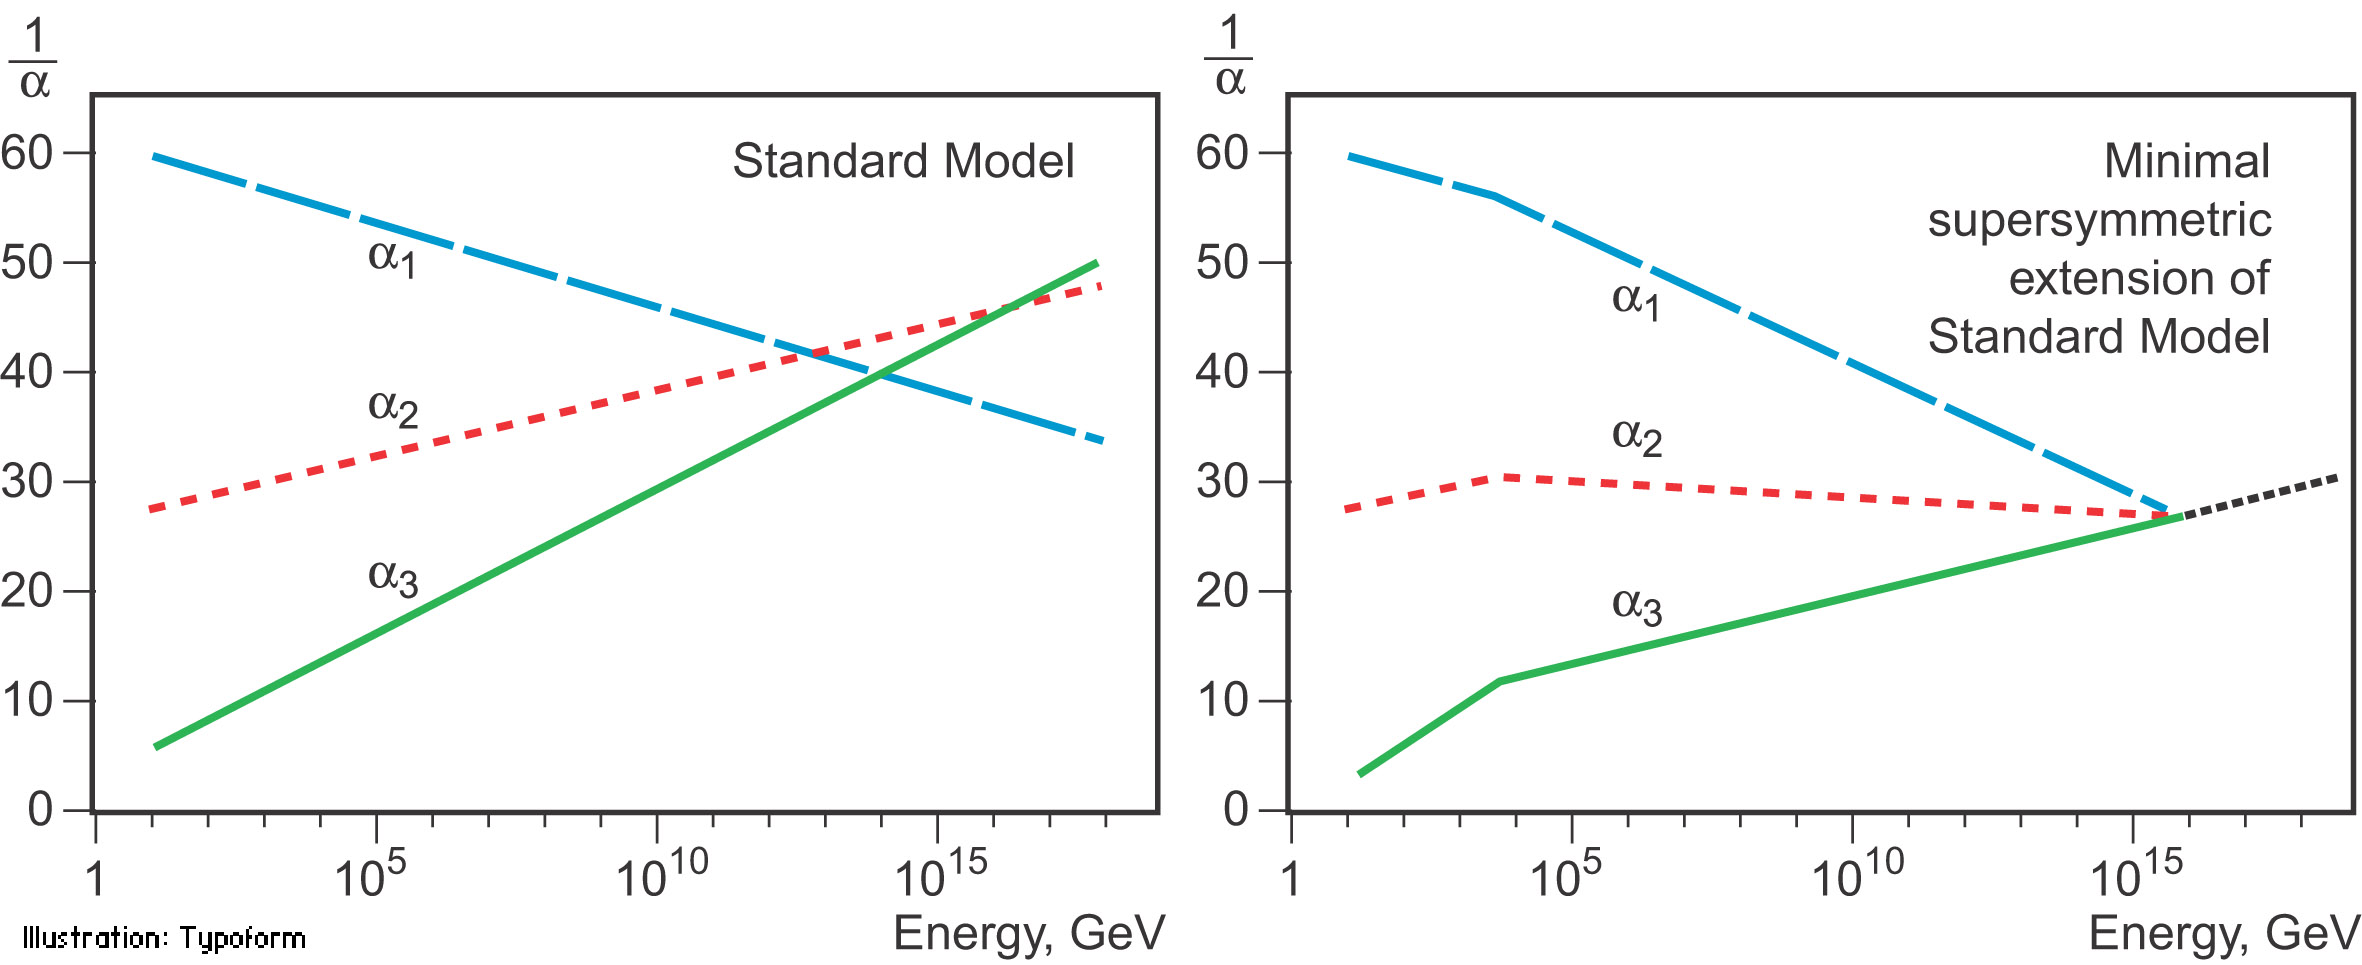
\includegraphics[width=1.0\linewidth]{figs/runningCouplingSusy}
  \caption[]%
  {Evolution of the inverse of the coupling constants of the
  electroweak $U(1)$, $\alpha_1$, electroweak $SU(2)$, $\alpha_2$, and
  strong force $SU(3)$, $\alpha_3$ for the \SM and \MSSM \cite{runningCoupling}}%
  \label{fig:runningCoupling}
\end{figure}

\subsection{The Minimal Supersymmetric Standard Model}
\label{sec:MSSM}

The \acf{MSSM} is a model that incorporates \SUSY with the \SM in a
way that adds the minimum number of new particles and interactions
\cite{Csaki:1996ks}. The \MSSM has 105 free parameters in total, a
significant increase from the 19 in the \SM. A summary of the extra
particles, \emph{sparticles}, introduced by the \MSSM is available in Tab.~\ref{tab:susy}.
The superpartners to the fermions are denoted with the same symbol as
their associated fermion with a tilde above. The weak sector is
extended within the \MSSM and the mixing of the new \SUSY fields
associated to the electroweak and Higgs bosons leads to
the existence of neutralinos, charginos and a total of five Higgs
bosons, including two that carry an electromagnetic charge. 
%Could add in more detail of the fields and things here but it's
%probably not relevant...

\begin{table}
\begin{tabular}{|l|c|c|c|}
%\hline 
Name & Sparticle & Spin & Charge, $q$ \\
\hline
Up-type squarks & $\tilde{u},\tilde{c},\tilde{t}$ & 0 & $+\frac{2}{3}$ \\
Down-type squarks & $\tilde{d},\tilde{s},\tilde{b}$ & 0 & $-\frac{1}{3}$ \\
Charged sleptons & $\tilde{e},\tilde{\mu},\tilde{\tau}$ & 0 & $\pm1$ \\
Sneutrinos & $\tilde{\nu_{e}},\tilde{\nu_{\mu}},\tilde{\nu_{\tau}}$ & 0 & 0 \\
\hline
%\hline
Gluino & $\tilde{g}$ & $\frac{1}{2}$ & 0 \\
Neutralinos &
$\tilde{\chi_{1}}^0,\tilde{\chi_{2}}^0,\tilde{\chi_{3}}^0,\tilde{\chi_{4}}^0$
& $\frac{1}{2}$ & 0  \\
Charginos & $\tilde{\chi_{1}}^{\pm},\tilde{\chi_{2}}^{\pm}$ &
$\frac{1}{2}$ & $\pm1$ \\
\hline
Neutral Higgs bosons & $h^0,H^0,A^0$ & 0 & 0 \\
Charged higgs bosons & $H^{\pm}$ & 0 & $\pm1$ \\
\end{tabular}
\caption{The extra particles introduced by the \MSSM. The symbol $h^0$
is typically used to denote the \SM Higgs boson.
% A subscript of
% $L$ or $R$ denotes the left or right-handed states respectively
\cite{Martin:1997ns}}
\label{tab:susy}
\end{table}
% table from mark

Unlike the \SM, the \MSSM permits lepton and baryon number violation,
the total numbers of leptons and baryons do not need to be conserved.
This could lead to interactions in which quarks can produce leptons,
such of interactions would allow protons to spontaneously decay.
However, stringent limits have been set on the lifetime of a proton,
$\tau>10^{33}$~years, that should exclude or heavily suppress this
kind of behaviour. This is dealt with in the \MSSM by introducing a
new conserved quantity known as \emph{R-parity}, $R$:
\begin{equation}
R\equiv (-1)^{3(B-L)+2s}
\end{equation}
where $B$ is the baryon number, $L$ the lepton number and $s$ the spin
of the particle. This leads to \SUSY particles having $R=-1$ and \SM
particles have $R=+1$. The consequence of this is that \SUSY particles
always decay to at least one other \SUSY particle. Additionally, any
\SUSY particles produced by \SM interactions must be produced in
pairs and vice versa. With R-parity conservation the \acf{LSP} is
stable. This fact allows it to fulfil the role of \DM in the case that
the \LSP is neutral. In most favoured \SUSY models the \LSP is
therefore typically taken to be a neutralino \cite{Farrar:1978xj}.
% R-parity - put a note on DM
% define lsp - neutralino in the case of DM

For the \MSSM to successfully solve the hierarchy problem an
additional constraint is applied to the \SUSY particles. As there is
no explicit mass hierarchy in the squark generations predicted in
\SUSY, the sparticles of the top-quark, the \emph{stop}, is typically
required to be the lightest of the squarks. This ensures maximal
cancellation of the contributions to the Higgs mass from the
top-quark, which couples most strongly to the Higgs in the \SM.
% light stops - to solve hierarchy problem

\subsection{Signatures of supersymmetry at the \LHC}

Despite the fact that \SUSY presents a promising extension to the \SM
there have been no significant experimental hints of its existence.
Searches for the evidence of \SUSY production have been performed in a
series of particle collider experiments, but have only resulted in
excluding possible regions of \SUSY parameter space. However, for
\SUSY to convincingly solve the hierarchy problem, it is expected to
present itself at the $O(1)$~TeV energy scale. This scale is just
starting to be explored by the \LHC. If \SUSY is to exist in the form
that is typically conceived it should therefore be evident in the
proton collisions produced by the collider.

The fact that there are a lot of different free parameters in the
\MSSM leads to a wide range of possible \SUSY phenomenologies.
However, constraints made by R-parity and naturalness
considerations help to limit the possible signatures. These
constraints typically lead to the pair production of \SUSY particles
that rapidly decay via \SM particles to a weakly interacting neutral \LSP. 
As the produced \SUSY particles have a reasonably high mass, this
leaves a significant missing momentum signature in any detector that
is looking for \SUSY signatures.
% R-parity, naturalness, neutralino lsp make it good for searching

As the \LHC is a hadron collider, the highest cross section \SUSY
production processes occur via the strong force \cite{Martin:1997ns}
\cite{SUSYxsections_NewAspectsof_pp_collisions}. These processes
result in the production of pairs of squarks or gluinos, the \SUSY
particles with colour charge, that predominantly decay via an even
number of \SM quarks to an \LSP. A Feynman diagram of typical squark
and gluino production and decay is shown in Fig.~\ref{fig:susyDecay}.
The resulting signature will usually be characterised by high energy
hadronic jets of \SM particles recoiling from invisible particles.

\begin{figure}
  \centering
  \subfloat[]{
    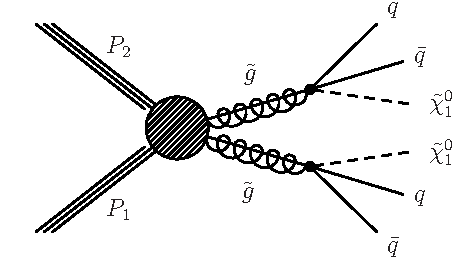
\includegraphics[width=0.4\textwidth]{figs/T1qqqq}
    \label{fig:susyDecayGluino}
  }~~~ 
  \subfloat[]{
    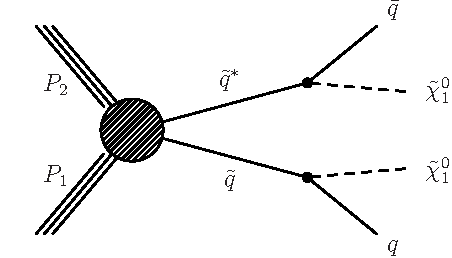
\includegraphics[width=0.4\textwidth]{figs/T2qq}
  }
  \caption{Representative \SUSY production and decay of gluinos, (a), or
  squarks, (b), in proton-proton collisions. The \SUSY particles decay
  to a weakly interacting neutralino, $\tilde{\chi_1}^0$, via \SM
  quarks \cite{smsTwiki}.}
  \label{fig:susyDecay}
\end{figure}

\subsection{Simplified models}

As there are a large number of parameters in the \MSSM there are many
different versions of the theory that can all result in different
\SUSY phenomenology. One of the things that has the biggest effect
when carrying out searches for \SUSY production is the mass hierarchy
of the particular model. To help to rationalise this the results of
\SUSY searches are typically interpreted within the context of
\emph{simplified models} \cite{Alwall:2008ag,Alves:2011wf}. These
models utilise a \SMS framework that typically consider only one
possible \SUSY decay per model. The simulated \emph{parent} \SUSY
particles and the \emph{daughters} that they decay to are kept at a
reasonable mass scale that is reachable by the search. All other \SUSY
particles are assumed to be at a much higher mass scale such that they
have no effect on the decay in question. An example of a decay
targeted by a simplified model with gluino parents and neutralino
daughters is in Fig.~\ref{fig:susyDecayGluino}. 

Searches for \SUSY are typically interpreted in different simplified
models with a wide range of parent and daughter masses. In the case
that no \SUSY signature is observed, the simplified models that are
excluded and those that are not allow limits to be set on the minimal
mass of different \SUSY particles within the context of the particular
simplified model. As the models separate out different possible \SUSY
production and decay mechanisms searches will typically interpret
their results in different models. Searches that look in a purely
hadronic final state, for example, will consider simplified models
that do not have leptons in the final state. Also, the type of search
that is successful at excluding some types of mass spectra is not as
successful at others. When the parent and daughter particles are very
close in mass, known as having a \emph{compressed spectrum}, the \SM
decay products carry very little energy. Searches for these types of
models therefore rely on \acf{ISR} or \acf{FSR} recoiling from the
invisible \SUSY system.

% With the standardised \SMS framework the interpretation of the results
% of \SUSY searches across the whole field is made simpl
%easy for outside interpretation

\subsection{Status of experimental searches for supersymmetry}

Signatures of \SUSY have been extensively searched for at previous
particle collider experiments including HERA ($ep$)
\cite{Aid:1996es,Butterworth:1992tc}, LEP ($e\bar{e}$)
\cite{Braibant:2003px} and the Tevatron ($p\bar{p}$)
\cite{Jaffre:2012gx}. These were then surpassed in most regions of
phase space by searches with the \CMS and ATLAS experiments with the
\LHC during Run~1. The \LHC is the first experiment to prove the
multi-TeV scale, where natural \SUSY is expected to lie. No hints of
\SUSY have yet been seen. The degree to which the $8~\tev$ Run~1
results have excluded the mass scales of different \SUSY particles
within a simplified model context can be seen in
Fig.~\ref{fig:run1Exclusion}.
%show lhc1 thing

\begin{figure}
  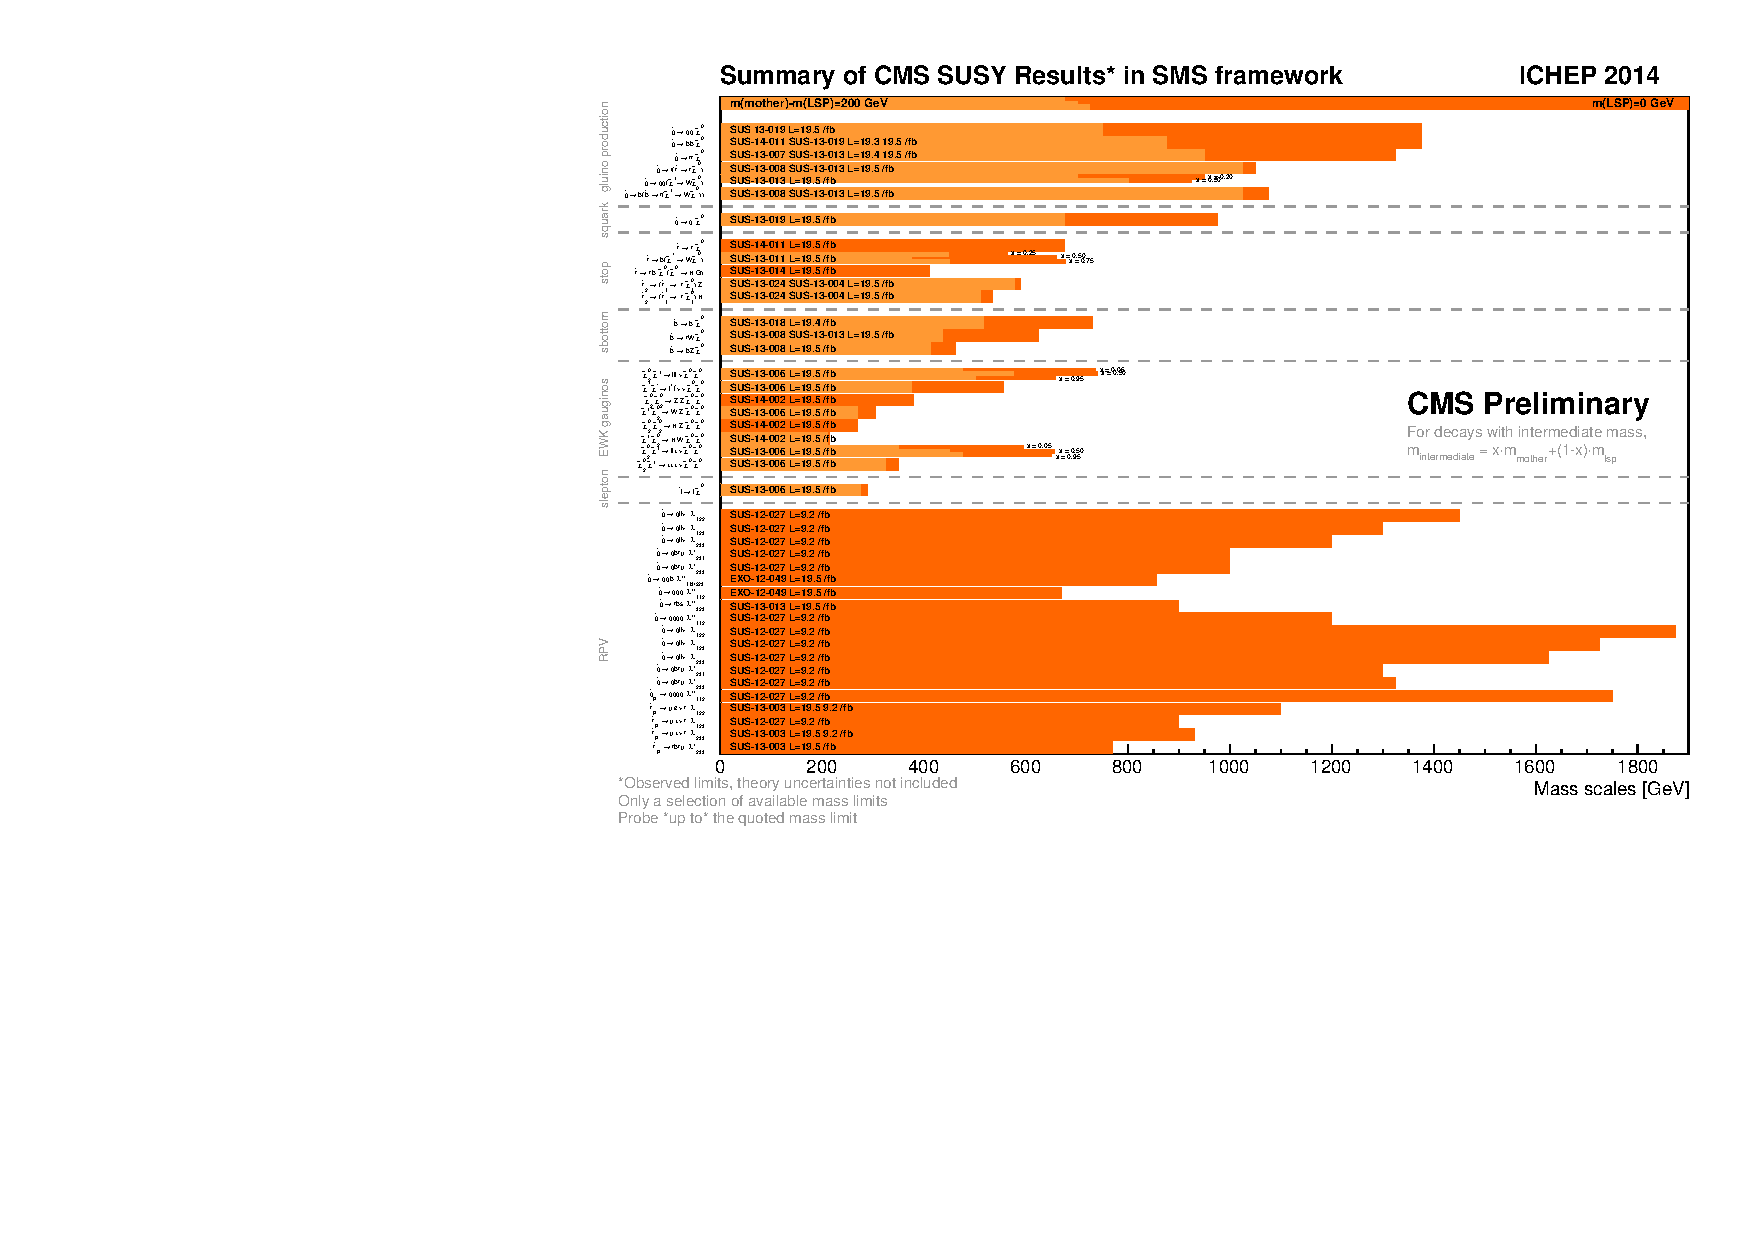
\includegraphics[width=1.0\linewidth]{figs/run1SusyExclusion}
  \caption[]%
  {Maximum exclusion limits for the mass of \SUSY parent particles for
  simplified models with an \LSP with 0~GeV mass (dark shades) or
  parent mass minus \LSP mass of 200~GeV (light shades) for a
  representative selection of simplified model topologies. The results
  were made with data collected by \CMS with $8~\tev$ centre of mass
  proton-proton collisions \cite{smsTwiki}.}%
  \label{fig:run1Exclusion}
\end{figure}

% Best exclusion limits for the masses of the mother particles for
% m(LSP) = 0 GeV (dark shades) and m(mother) - m(LSP) = 200 GeV (light
% shades); for each topology, for all results. In this plot, the lowest
% mass range is m(mother)=0, but results are available starting from a
% certain mass depending on the analyses and topologies. Branching
% ratios of one are assumed, values shown in plot are to be interpreted
% as upper bounds on the mass limits, see the analyses documentations
% for details. (Note: theory uncertainties not included.)

For \SUSY at the electroweak scale to exist in a sensible form that
convincingly solves the problems described in Sec.~\ref{sec:bsm} it
should be observable during Run~2 of the \LHC that probes even higher
energies with $13~\tev$ proton collisions. If no evidence presents
itself, the typical assumptions made when building \SUSY models will
have to be reassessed.


  \chapter{The CMS experiment at the LHC}
\label{chap:detector}

\chapterquote{Traditional scientific method has always been, at the
very best, 20-20 hindsight. It's good for seeing where you've been.
It's good for testing the truth of what you think you know, but it
can't tell you where you ought to go.}%
{Robert M. Pirsig, Zen and the art of motorcycle maintenance}

The \LHC is one of the largest machines ever built. It exists within a
27~km tunnel $\sim 100$~m$)$ underground on the border of France and
Switzerland. Around the ring of the \LHC are built a series of
detectors that can record in a high level of detail the result of high
energy particle collisions produced by the collider. This chapter
will focus on the details and performance of \CMS, a multi-purpose
detector optimised to search for new, as yet undiscovered, particles.

\section{The LHC}
\label{sec:lhc}

The \LHC is a hadron collider designed to collide protons and lead
ions at centre of mass energies up to 14\tev, the highest ever achieved by such a
machine
\cite{Evans:2008zzb,CERN-2004-003-V-1,CERN-2004-003-V-2,CERN-2004-003-V-3}.
The proton-proton collisions are most utilised for direct searches for
new physics and therefore take up the vast majority of the \LHC's
running time. 

To bring protons up to the $6.5~\tev$ required in Run~2 of the \LHC
they are accelerated through a series of stages. Hydrogen atoms are
initially stripped of their electrons and accelerated to 50\mev by
\ac{LINAC2}. The energy is then increased to 1.4\gev by the \ac{PSB}
before being injected into the \ac{PS} which boosts the energy up to
26\gev. A final kick up to 450\gev is provided by the \ac{SPS}. This
chain of accelerators also collect the protons into bunches that are
either 25~ns (from Run~2 onwards) or 50~ns apart (during Run~1 and
early stages of Run~2). These bunches are then injected into the \LHC,
in which they are steered by around 1200 superconducting dipole
magnets while being accelerated up to $6.5\tev$ with \ac{RF} cavities.
Once the beam has reached the intended energy and is stable, protons
are collided at four different points on the ring, around which are
built the four major \LHC detectors, ALICE \cite{Aamodt:2008zz}, ATLAS
\cite{Aad:2008zzm}, LHCb \cite{Alves:2008zz} and \CMS
\cite{Chatrchyan:2008aa}.  A representation of this accelerator
complex and the location of the detectors can be seen in
Fig.~\ref{fig:lhc}.

\begin{figure}
  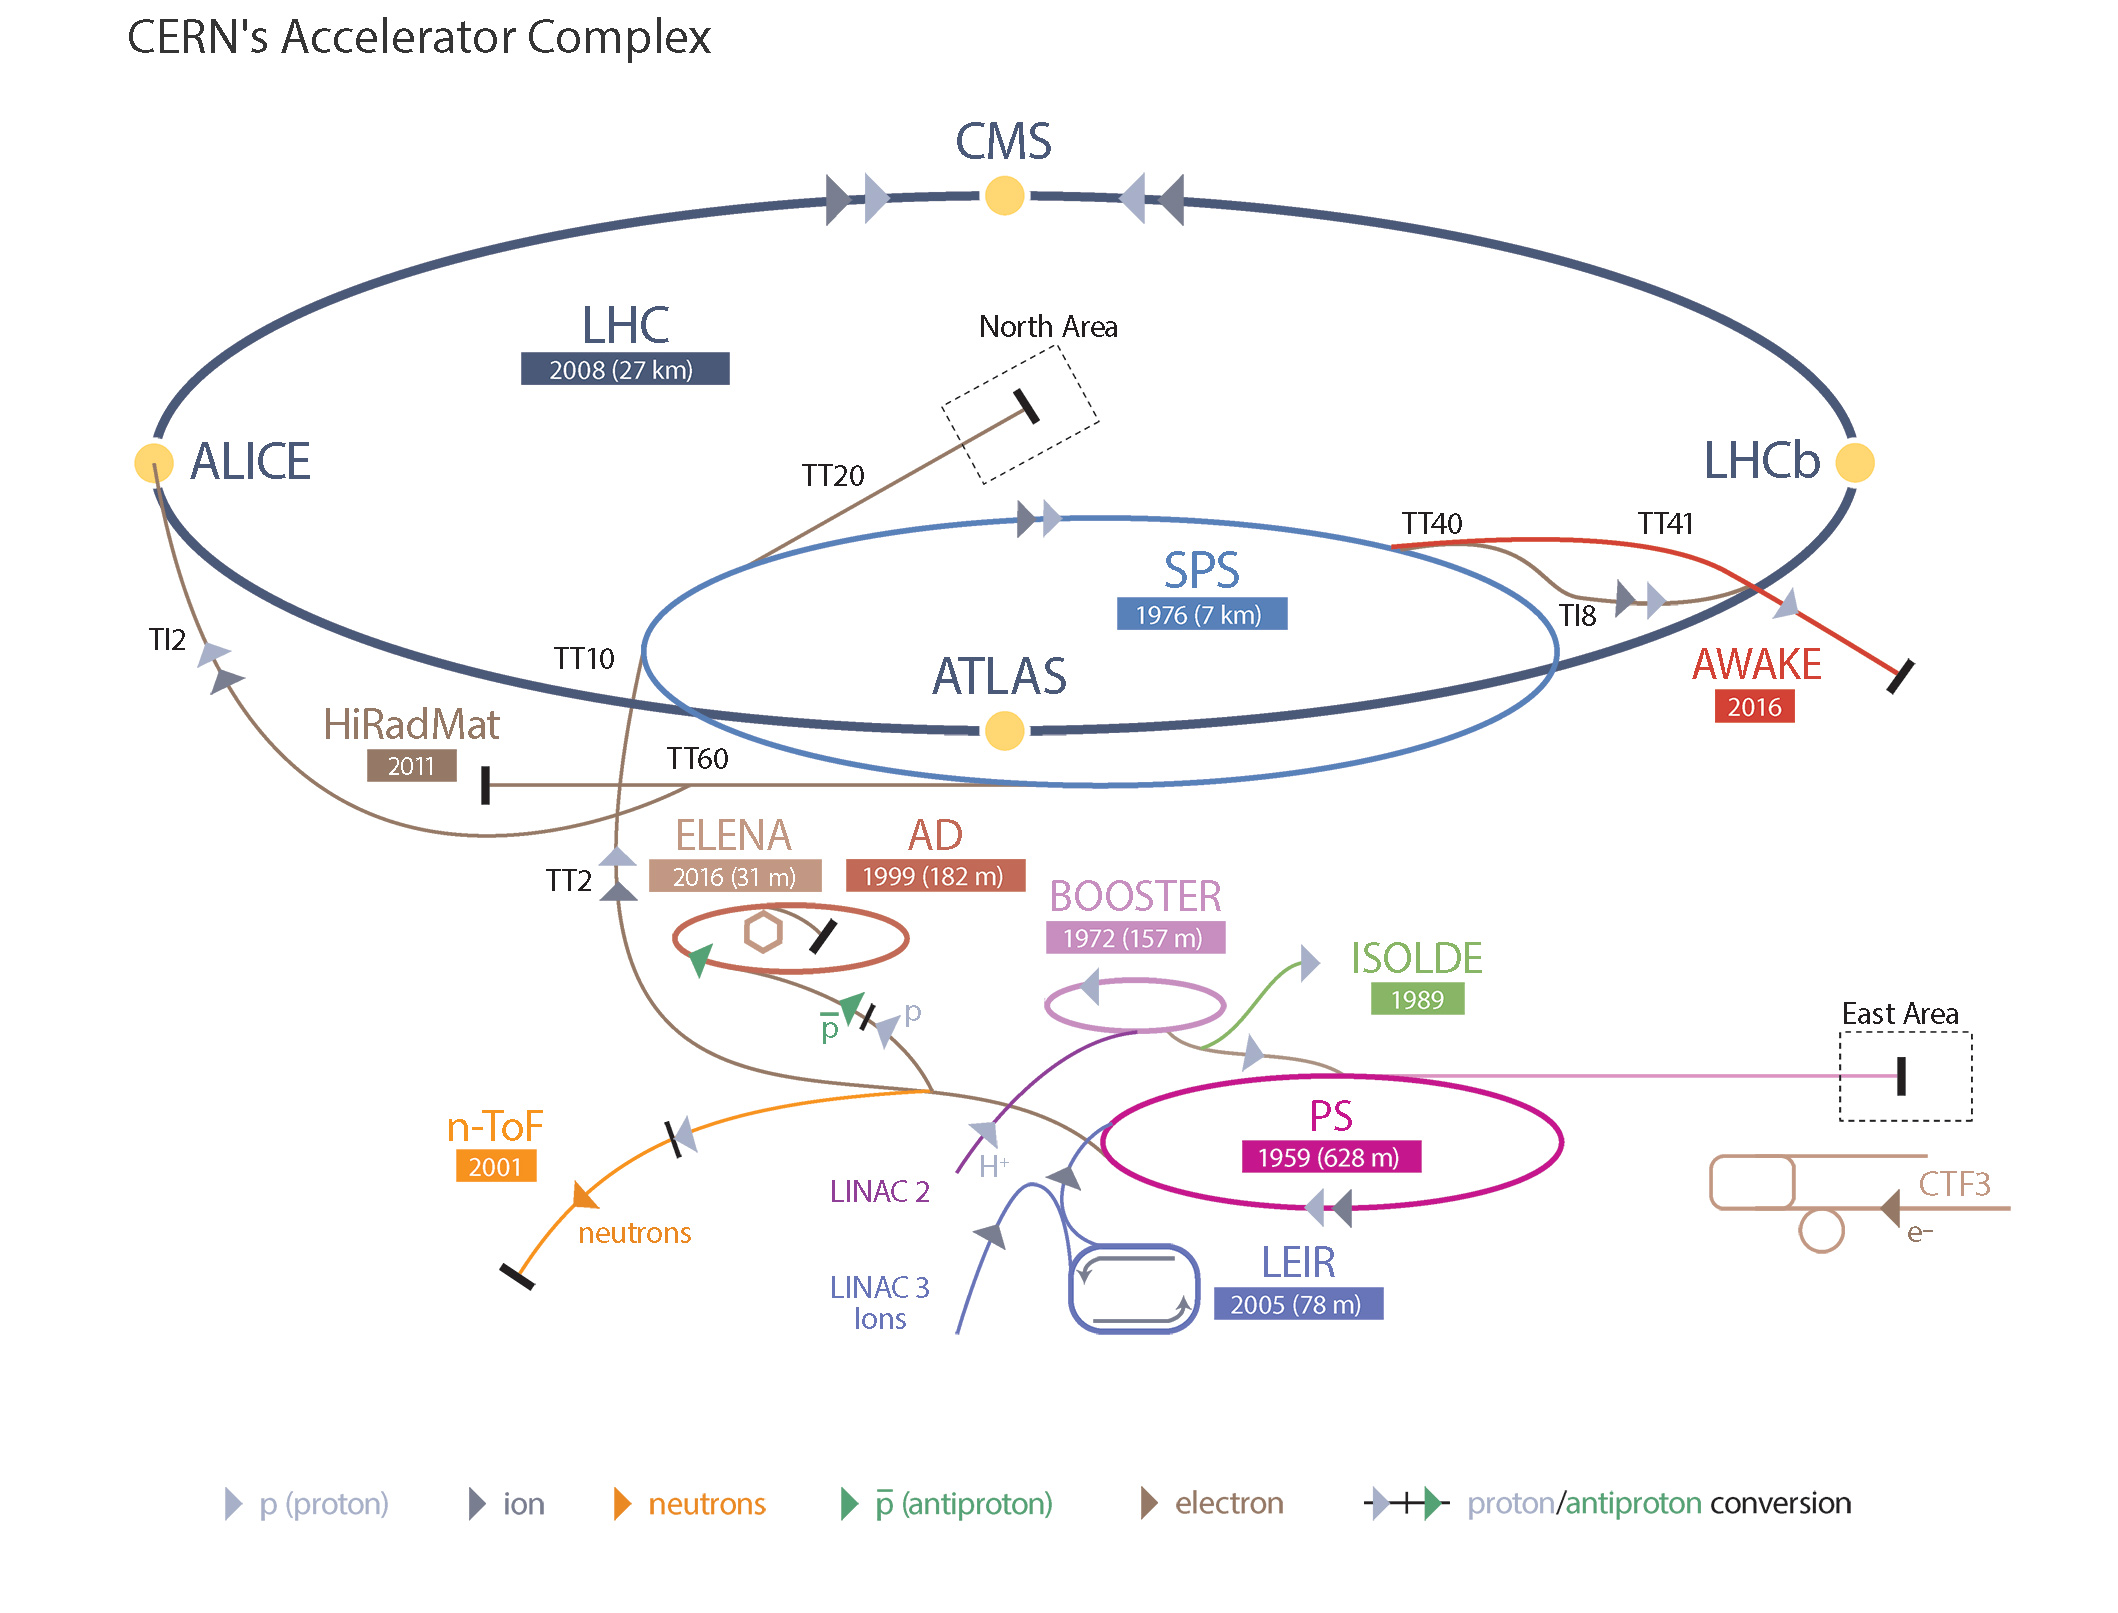
\includegraphics[width=\largefigwidth]{figs/LHC_default}
  \caption[]%
  {A representation of the CERN accelerator complex that help
  accelerate protons to record energies within the \LHC
  \cite{stfc:lhc}}%
  \label{fig:lhc}
\end{figure}

As well as attaining record breaking energies, the \LHC is designed to
collide hadrons at a very high luminosity, with a bunch collision rate
of up to $40~\mhz$ \cite{Evans:2008zzb}. This is necessitated by the
fact that the rate at which electroweak scale processes
occur in proton collisions is significantly lower than their
associated backgrounds, demonstrated in Fig.~\ref{fig:xsecs}.
The \LHC is therefore designed to run at an instantaneous
luminosity approaching $10^{34}$cm$^{-2}$s$^{-1}$ to maximise the occurence of
these rare processes. Along with the high collision rate, this
luminosity is achieved by squeezing the proton bunches to increase the
number of simultaneous collisions per bunch crossing, the extra
simultaneous collisions are known as \PU.  The \LHC has typically
operated with a \PU of $\sim10\mbox{-}20$, however to increase the
luminosity in the future this value will be increased up to a \PU of
O(100).
% , presenting a significant challenge for current and future 
% physics analyses at the \LHC.

\begin{figure}
  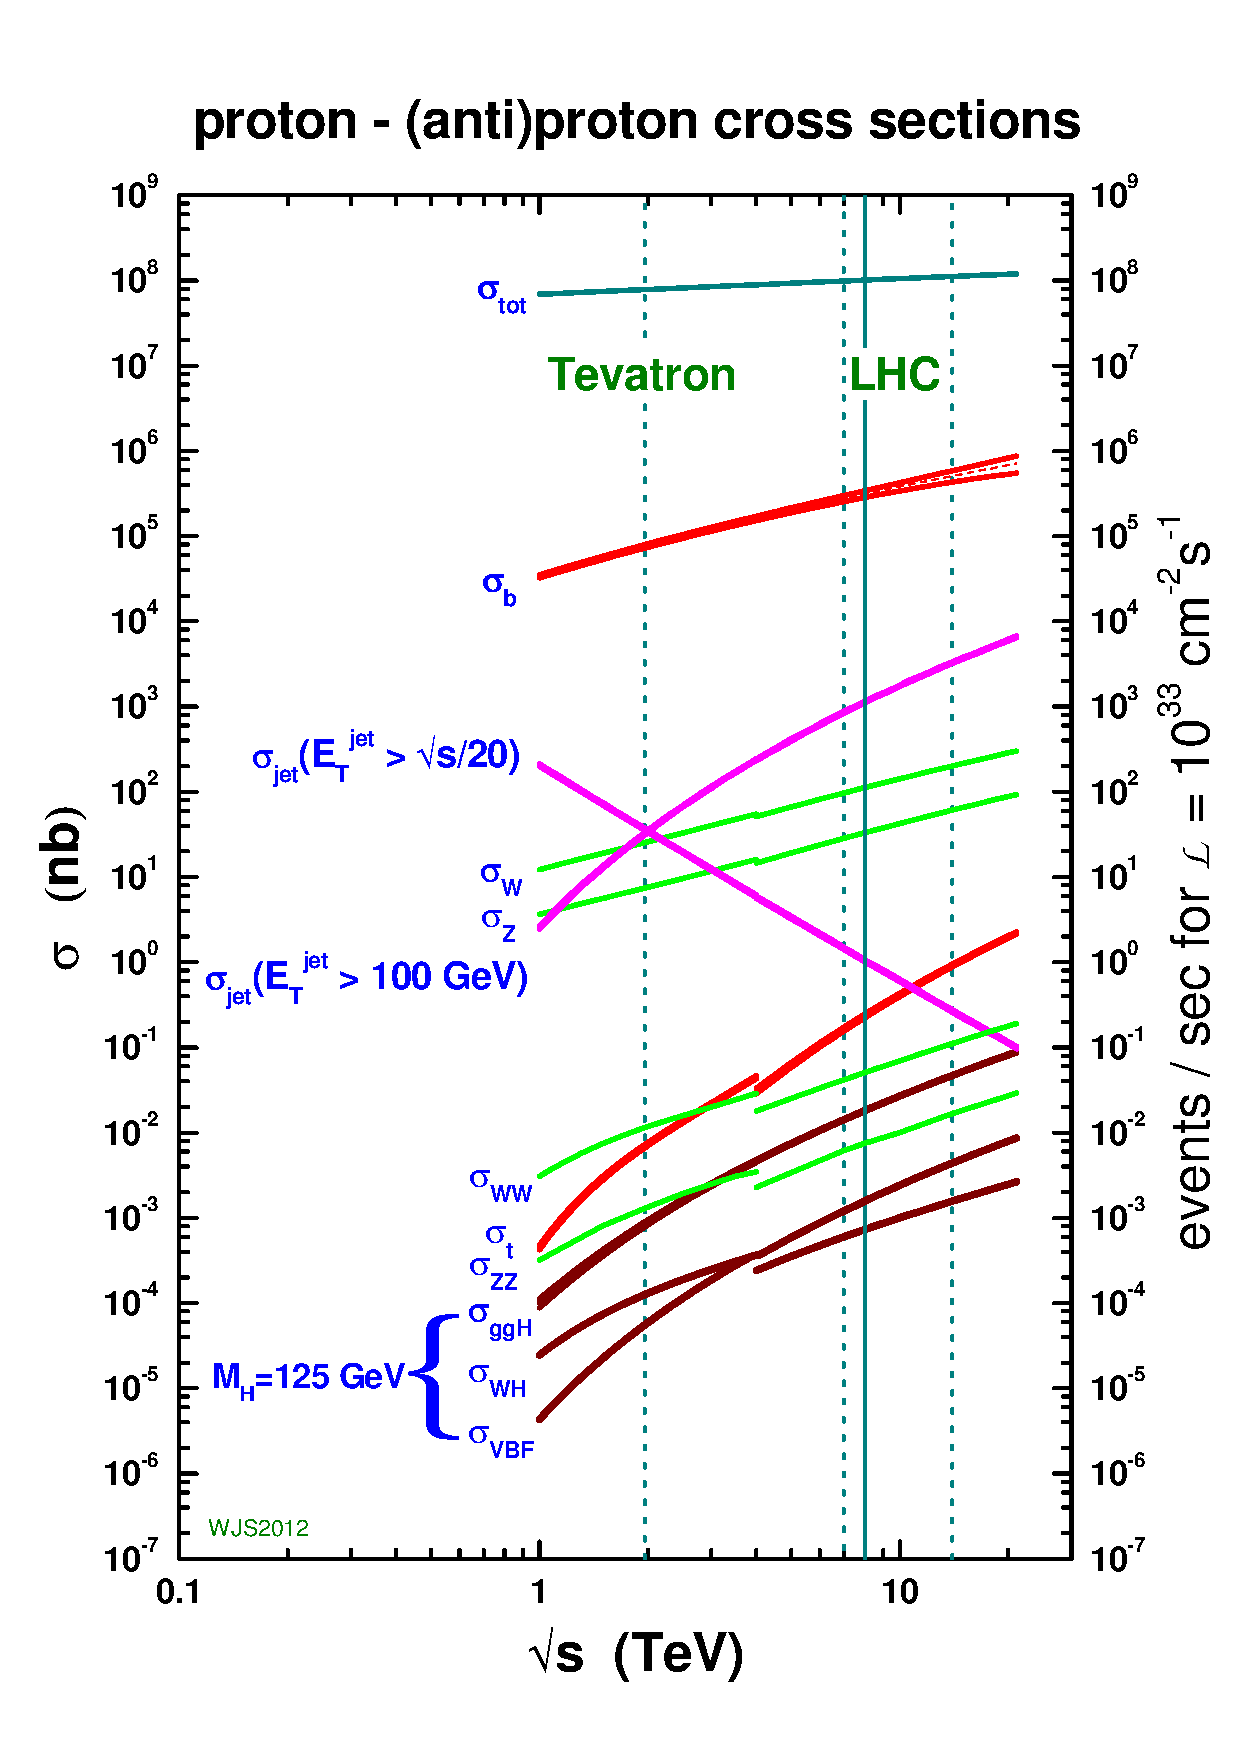
\includegraphics[width=\mediumfigwidth]{figs/crosssections2012_v5}
  \caption[]%
  { The cross sections for various standard model processes as a
  function of proton collider energy, demonstrating the importance of
  high luminosities when observing electroweak scale processes
  \cite{stirlingCrossSec1}.}%
  \label{fig:xsecs}
\end{figure}

During Run~1 of the \LHC, from 2010-2013, a total of $23.3~\ifb$ of
data were collected at centre of mass energies of $\sqrt{s}=7~\tev$ and
$8~\tev$. After this there was a period of shutdown in which the \LHC
and the detectors underwent a series of upgrades. Run~2 then began in
2015 with the collision of protons at $\sqrt{s}=13~\tev$. During 2015 a
total of $4.3~\ifb$ were collected at this energy. So far in 2016 the
\LHC has delivered $34.6~\ifb$, a record breaking number of collisions
at the highest ever recorded energies. 

\section{The CMS detector} \label{sec:cms}

The \CMS detector is one of two multipurpose detectors built around
proton beam collision points, the other being ATLAS. It is situated at
Point 5 on the \LHC, as visibile in Fig.~\ref{fig:lhc}. The key goals
of the \CMS detector at its conception were the discovery of the \SM
Higgs boson and searches for generic signatures of \BSM physics. In \CMS the
results of collisions are measured with a series of subdetectors,
built within and around a $3.8~$T superconducting solenoid. They are designed to
track, identify and record the energy of all non-neutrino \SM particles
\cite{Bayatian:2006zz}. With its comprehensive solid
angle coverage, \CMS is well suited to inferring the existence of
weakly interacting particles through the momentum imbalance of visible
particles. This is particularly relevant when searching for \BSM
physics.

\begin{figure}
\begin{center}
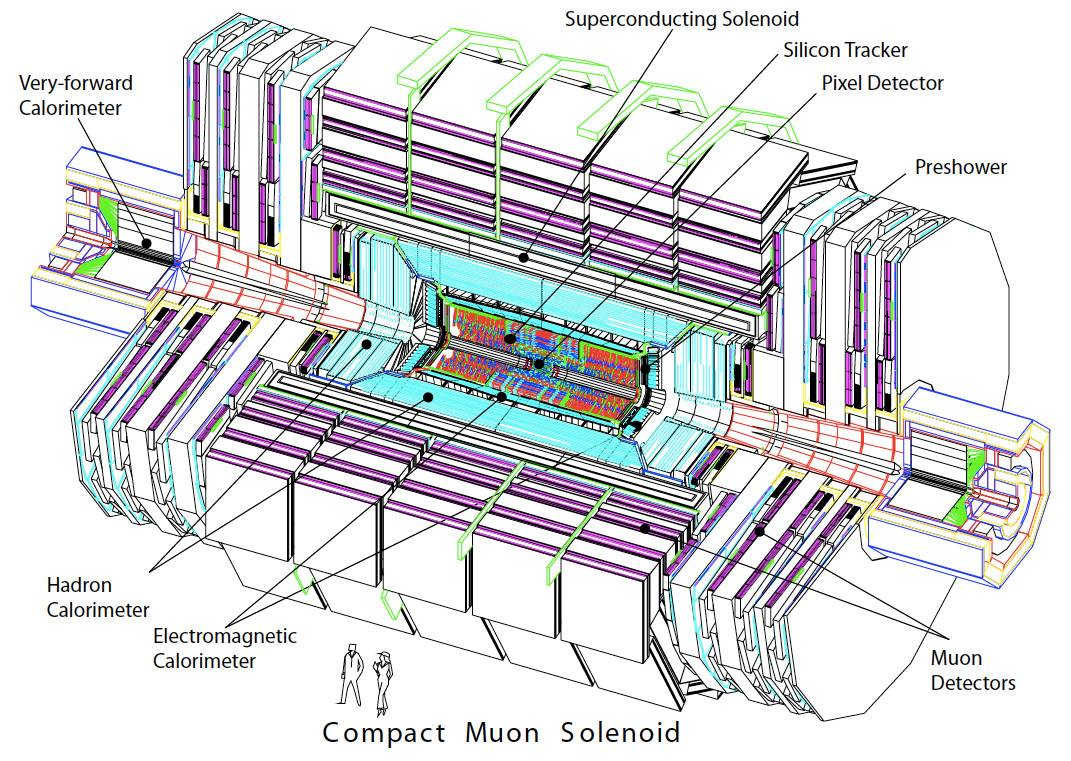
\includegraphics[width=0.8\linewidth]{figs/cms_detector} \end{center}
\caption{An internal view of the \CMS detector
highlighting the key detecting components \cite{Bayatian:2006zz}}
\label{fig:CMS} \end{figure}

A representative view of \CMS and its components can be seen in
Fig.~\ref{fig:CMS}. The detector is designed in a series of
cylindrical layers of subdetectors working out from the central point,
where the proton collisions occur. The first layer consists of the
silicon tracking system. This tracker is designed to allow the
reconstruction of the trajectory of charged particles produced in the
collision point as they move through the magnetic field. The degree to
which the path of these particles is bent allows for an accurate
determination of their momenta. The next layer beyond the silicon
tracker is the \ECAL, which is designed to absorb and measure the
energy of electrons and photons. Surrounding this is the \HCAL that
absorbs the remaining hadronic particles that have punched through the
\ECAL. Built around the tracker and calorimeters is the superconducting
solenoid. In the final layer are the muon chambers and iron return
yoke. The chambers are designed to detect the presence of muons that
will not be absorbed by the central components of the detector. The
data from all these subdetectors are read out by dedicated front end
electronic. They are then passed through the \CMS trigger system which
selects the most promising data to be kept and stored for ``offline''
processing. 

Measurements of physical quantities made by \CMS are typically
interpreted in a three dimensional coordinate system that originates
from the centre of the detector. The $x$-axis points south, to the
centre of the \LHC ring, the $y$-axis points vertically upwards and
the $z$-axis points along the direction of the \LHC beam pipe. It is
then helpful to define the azimuthal angle $\phi$ which is in the
$x$-$y$ plane and measured relative to the $x$-axis. Measurements of
momentum and energy in this plane are described as transverse and
known as \pt and \Et respectively. The polar angle $\theta$ is then
defined as relative to the $z$-axis. This angle is used to construct
the pseudorapidity, defined as $\eta=-ln(tan(\theta/2))$. Distances in
the $\eta$-$\phi$ plane is then given as $\Delta R =
\sqrt{\Delta\phi^2+\Delta\eta^2}$.

\subsection{The tracker} 

The \CMS inner tracking system is designed to accurately determine the
trajectories of charged particles produced in hadron collision events
\cite{Karimaki:368412}. In the presence of the strong magnetic field
provided by \CMS's solenoid, the curvature of these tracks can be used
to reconstruct momenta with a resolution between $1.5\%$ and $3\%$ for
$p_T\sim 100$~GeV charged particles. The tracker is also capable of
tracking \mbox{$p_T>1$~GeV} charged particles with an efficiency
greater than $99\%$ \cite{Bayatian:2006zz}. Along with this, the
spatial resolution of the tracker is such that the points of origin of
event decay products can be inferred within $10$~$\mu$m. Together,
this allows the performance of \CMS to extend up to very high levels
of \PU.% \cite{CMSTrackPerformance}.

The tracker is required to operate in a challenging, high radiation
environment. Additionally, in an ideal detector the particles produced
in collisions are solely absorbed by the calorimeters. The tracker
must therefore consist of as little material as possible. To achieve
the high level of precision and fast response time required given
these conditions, the tracker utilises silicon technology. As charged
particles pass through doped silicon an electron-hole pair is
produced. In the presence of an electric field this gives rise to a
pulse of electrical current in the previously resistive silicon. This
behaviour is utilised by the tracker in a series of silicon pixel and
strip detectors covering all angles in \phi and extending up to
$|\eta|<2.5$. The tracker's layout is visible in
Fig.~\ref{fig:tracker}. 

\begin{figure}
\begin{center}
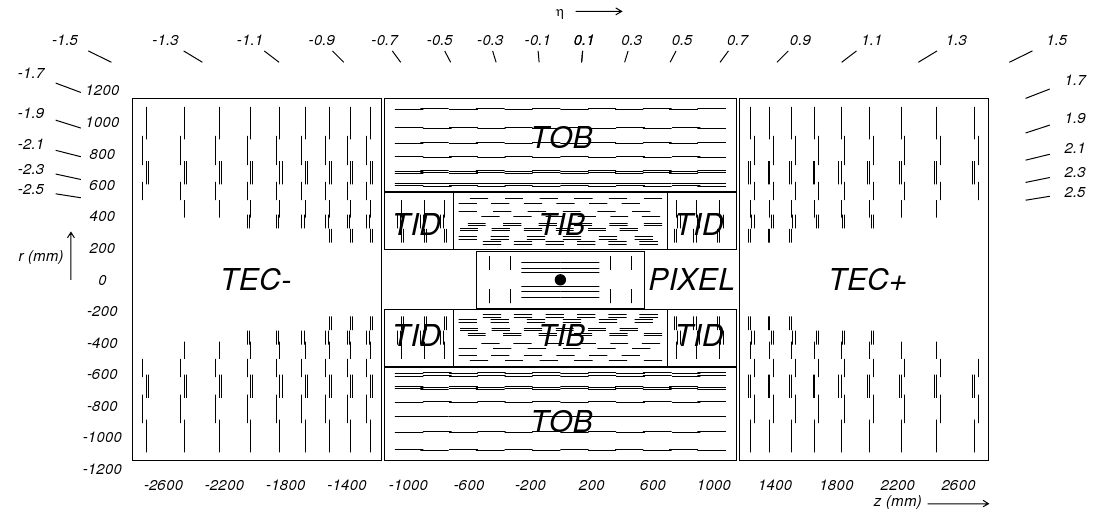
\includegraphics[width=0.8\linewidth]{figs/cmstracker} \end{center}
\caption{ A schematic of a cross section through the \CMS tracker.
Detector modules are represented by different lines \cite{Chatrchyan:2008aa}}
\label{fig:tracker} \end{figure}

The pixel detector is the high granularity component of the tracking
system that sits closest to the interaction point, covering the
pseudorapidity region $|\eta|<2.5$. It consists of three cylindrical
layers of hybrid pixel detector modules that are complemented by two
disks of pixel modules on each side. The pixel detector makes use of
66 million pixels covering an area of $\sim 1$~m$^2$ to give the
tracker its excellent spatial resolution of $15$-$20$~$\mu$m in both
the $r$-$\phi$ and $z$ direction. This resolution is essential for a
precise determination of the position of collision event vertices and
for the observation of vertices displaced from this origin that can be
used to identify particles such as hadrons containing $b$-quarks.

Surrounding the pixel detector is the silicon strip tracker that
covers the region up to $|\eta|<2.4$. It consists of three different
subsystems built from 9.6 million silicon strips that cover an area of
198~m$^2$. Each of these strips are 10-20~cm long and 80-180~$\mu$m
wide. Working out from the centre the subsystems are the
Tracker Inner Barrel and Disks (TIB/TID), the Tracker Outer Barrel
(TOB) and the Tracker End Caps (TEC). They are arranged in a geometry
that maintains a good degree of coverage across all angles and can be
seen in detail in Fig.~\ref{fig:tracker}. Along with the spatial
resolution provided by the pixel detector the silicon strip tracker
adds enough modules to reconstruct the trajectory of particles to the
required high level of precision.

\subsection{The electromagnetic calorimeter} 

The \ECAL is constructed from $\sim 75~848$ lead tungstate (PbWO$_4$)
scintillating crystals covering the region $|\eta|<3$ \cite{CMS:1997ema}. It is
designed to absorb electrons and photons and emit light proportional to the
energy deposited. This light is detected by custom photodiodes that
perform well in high magnetic fields. This is achieved in a way which
is fast, radiation resistant and with a high granularity. 

The \ECAL is divided into the \ac{EB} which covers the region
$|\eta|<1.479$ and the \ac{EE} which covers the region
$1.479<|\eta|<3.0$. Additionally, built just before the \ac{EE} in the
region $1.653<|\eta|<2.6$ is the Preshower. Unlike the other
components, which are predominantly PbWO$_4$ crystals, the Preshower is
a lead and silicon sampling calorimeter. Its main aim is to improve
the position resolution of particles in the forward direction and help
to distinguish collinear $\pi^0$ decays from high energy photons
\cite{Chatrchyan:2008aa}. This layout of the \ECAL can be seen in
Fig.~\ref{fig:ecal}.

\begin{figure}
\begin{center}
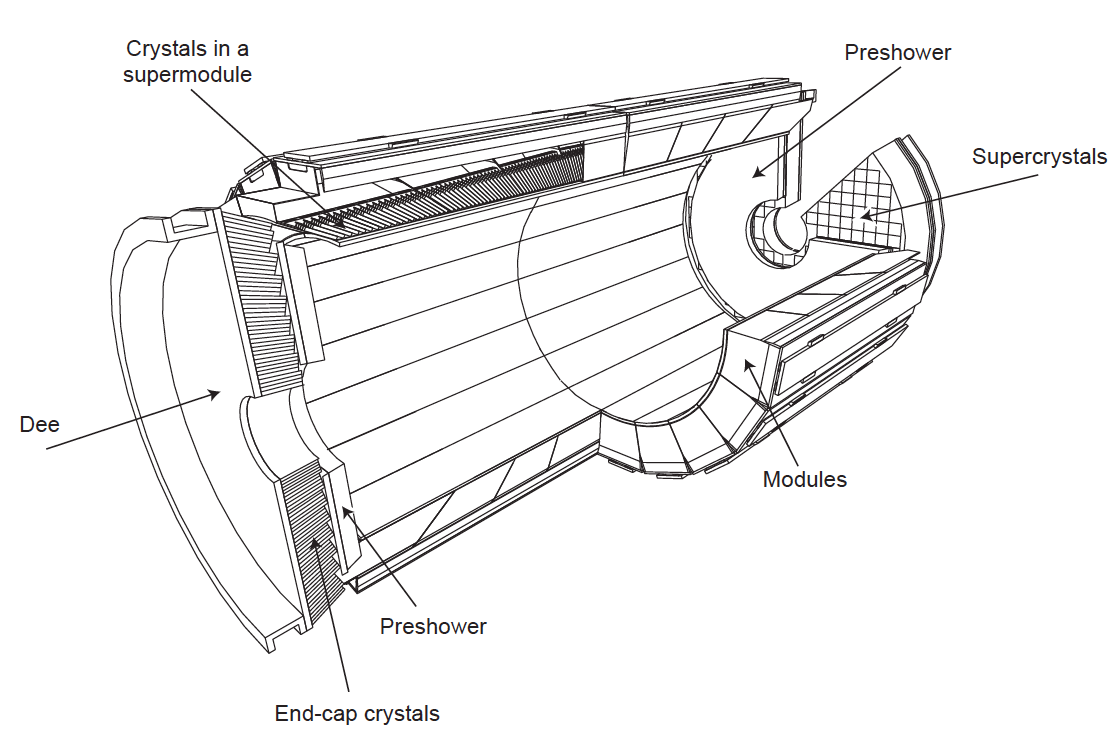
\includegraphics[width=0.8\linewidth]{figs/ecal_colorless} \end{center}
\caption{ A cutaway diagram of the \CMS \ECAL. All the key components,
including the barrel and endcap crystal layouts, are displayed
\cite{Chatrchyan:2008aa}}
\label{fig:ecal} \end{figure}

As high energy electrons or photons enter one of the \ECAL's crystals
they initiate an electromagnetic shower. This results in a cascade of
lower energy particles that undergo bremsstrahlung and pair
production.  These charged particles ionise atoms in the crystal which
then emit scintillation light as they de-excite. As the crystals are
transparent, this light can be measured by avalanche photodiodes and
vacuum phototriodes which convert it into an electronic current. The
magnitude of this current is then proportional to the energy deposited
in the crystal and can be used to accurately infer the total energy
deposited. Irradiation of the crystals decreases their transparency
over time. To counteract this a time dependent calibration is carried
out for each of the crystals with a laser of wavelength
$\lambda=440$~nm. 

Measurements in a test beam in the absence of a magnetic field have
measured the PbWO$_4$ crystals to have a resolution, $\sigma_E$, given
by the following formula \cite{1748-0221-2-04-P04004}:
\begin{equation} \label{eq:ecalres}
\left(\frac{\sigma_E}{E[\gev]}\right)^2=\left(\frac{2.8\%}
{\sqrt{E[\gev]}}\right)^2+\left(\frac{12\%}{E[\gev]}\right)^2+(0.30\%)^2.
\end{equation} 
In this equation $E$ denotes the energy of the incident
particle. The first term encapsulates uncertainties from fluctuations in the
scintillation light. The second term takes account of noise in the
electronics and digitisation. The final term then covers any
non-uniform longitudinal response or inter-calibration errors. 

\subsection{The hadronic calorimeter} 

The final layer of calorimetry in \CMS is the \HCAL \cite{CMS:HCAL}.
It is designed to absorb hadrons that have punched through the \ECAL.
It is a sampling calorimeter that is constructed from brass absorbers
interleaved with scintillating plastic tiles covering $|\eta|<3$. The
scintillations are read out with hybrid photodiodes via wavelength
shifting fibres.  Additionally, the hadronic calorimetry is extended
up to $|\eta|<5.2$ with the \ac{HF}, made from steel absorber with
quartz scintillating fibre. 

The brass absorbers are arranged in plates that are interspersed with
plastic tiles. Incident particles induce hadronic showers in the
brass layers that produce scintillating light in the plastic. This
light is collected by wavelength-shifting fibres which transfer the
signal to on-detector amplifiers for read-out. Brass has the advantage
of being non-magnetic and having the short nuclear interaction length
of 16.42~cm. In the \ac{HF} steel replaces the brass and quartz fibre
replaces the plastic due to the very high radiation environment
present in the forward region of the detector. The total time to
collect a \HCAL signal pulse is large with respect to the collision
rate of the \LHC. Only $68\%$ of the pulse is collected within 25~ns.
This leads to cases of \ac{OOTPU} where signal from a bunch
crossing can influence the read out of future bunch crossings.

The subdetectors that make up the \HCAL along with the \ac{HF} can be
seen in Fig.~\ref{fig:hcal}. Within \CMS's solenoid is the \ac{HB},
which extends up to $|\eta|<1.3$, and the \ac{HE}, covering
$1.3<|\eta|<3.0$. They are segmented in \eta-\phi towers with a size
of $0.087\times0.087$ in the \ac{HB} varying up to $0.17\times0.17$ in
some areas of the \ac{HE}. The \ac{HB} towers are lined up with
$5\times5$ arrays of \ECAL crystals and each read-out individually. On
its own the \ac{HB} provides between $5.8$ and $10.6$ interaction
lengths of absorber while the \ac{HE} provides $\sim10$ interaction
lengths. Beyond the magnetic coil is the \ac{HO} that increases to a
minimum of $11.8$ the interaction length in line with the \ac{HB}. The
magnetic coil acts as an absorber for the scintillators in the \ac{HO}
that absorbs any late-starting or highly-penetrating showers.

\begin{figure}
\begin{center}
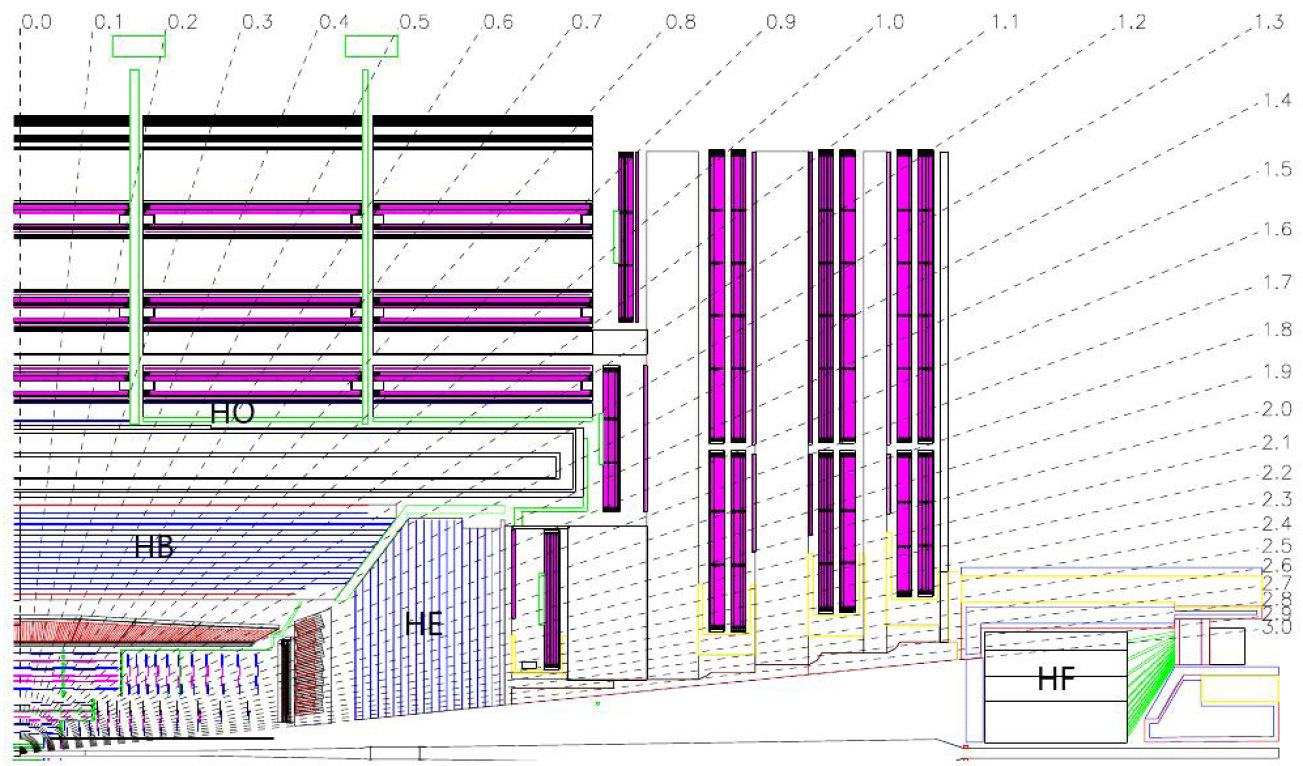
\includegraphics[width=0.8\linewidth]{figs/cms_HCAL} \end{center}
\caption{ A schematic of the \CMS \HCAL. The locations of the hadron
barrel (HB), endcap (HE), outer (HO) and forward (HF) calorimeters are
displayed \cite{Chatrchyan:2008aa}}
\label{fig:hcal} \end{figure}

The combined resolution, $\sigma_E$ of the \ECAL and \HCAL when
considered together have been measured in a test beam as
\cite{Abdullin:2008zzb}: 
\begin{equation} \label{eq:hcalres}
\left(\frac{\sigma_E}{E[\gev]}\right)^2=\left(\frac{84.7\pm1.6\%}
{\sqrt{E[\gev]}}\right)^2+(7.4\pm0.8\%)^2.  
\end{equation} 
In this equation $E$ is the energy of the incident particle. An
in-situ calibration is also performed with a UV laser and
$^{137}$Cs$/^{60}$Co sources that can be inserted into the scintillation
tiles in the \ac{HB} and \ac{HE}.

\subsection{The Muon System} As muons are unlikely to be absorbed in
the \ECAL and \HCAL, a muon system is built into the iron return yoke
that surrounds the solenoid.  This consists of wire chambers
containing ionising gas that allows the measurement of muon momenta
with a greater than $1\%$ precision
\cite{CMS_Overview_Chatrchyan:2008aa}.

\subsection{The Trigger and Data Acquisition System}
\label{sec:triggers} The rate of collisions at the LHC is so high that
it would be impossible to reconstruct and store the results of all
collision events. As the majority of the collisions are soft QCD
processes, they are not useful in the search for new physics at the
electroweak energy scale. This necessitates a multi-level trigger
system that is designed to pick out and store only high centre-of-mass
physics processes. The Level 1 Trigger (L1T) is the first component of
the trigger system and is made from custom FPGA computational boards
situated close to the detector. This uses coarse information from the
calorimeters and muon system to reduce the event rate from $20$MHz
(during Run 1) to $\sim100$kHz. The data from the subdetectors are
then passed to the High Level Trigger (HLT), which uses full detector
information to reconstruct the events and reduce the data rate to
$\sim1$kHz. The remaining events are then fully reconstructed and
stored at various Grid sites \cite{GridTechDesign}.



  \chapter{Event reconstruction and simulation}
\label{chap:reconstruction}

After the result of proton collisions have been observed in the
various subdetectors that comprise \CMS, the physical objects produced
in each collision event are reconstructed. Through this reconstruction
an overall analysis of the underlying physical process can be carried
out. To aid in classifying the types of collision events, \MC
simulations are also carried out. The reconstruction algorithms and
simulations that are relevant to the search for supersymmetry
presented in this thesis are described in this chapter.

\section{Tracks and vertices}
\label{sec:tracks_reco}

As charged particles pass through the \CMS tracker they leave energy
deposits, known as \emph{hits}, in each layer. These hits are
reconstructed as tracks with the \ac{CTF} algorithm
\cite{Chatrchyan:2014fea}, which tries to associate hits that belong
to a single charged particle. This allows for the determination of the
path taken by the charged particle, its \emph{track}. The curvature of
the particle as it passes through the magnetic field is then used to
determine its momentum. The steps of the algorithm are as follows:

\begin{itemize}
\item{Initially two or three hits in the inner layers of the tracker
are taken as seeds for initial track candidates. Quality
criteria are applied on the selected hits that retain only promising
seeds.} 
\item{Each seed is extrapolated along the expected trajectory using a
Kalman filter \cite{Fruhwirth:1987fm} with a helical tracking
hypothesis. This allows the seeds to be associated with hits in an
outer tracker layer while taking account of uncertainties in the
measurement.} 
\item{The extrapolation is carried out recursively into the subsequent
tracker layers until the outer-most layer, or another
stopping condition, is reached.} 
\item{Of the tracking candidates that are found, additional quality
criteria are required to reject fake tracks.}
\item{This series of steps is repeated up to six times with the hits
associated to identified tracks removed after each iteration. }
\end{itemize}

Track reconstruction efficiencies for a variety of charged particles
are shown in Fig.~\ref{fig:tracks_reco} as a function of \pt and
$\eta$. In the central region of the detector all particles with a \pt
from 10 to 100~\gev are reconstructed with a 90-100\% efficiency. In the
forward detector region this efficiency remains above $\sim80\%$.
%fake rate? leave out for now...

\begin{figure}
\begin{center}
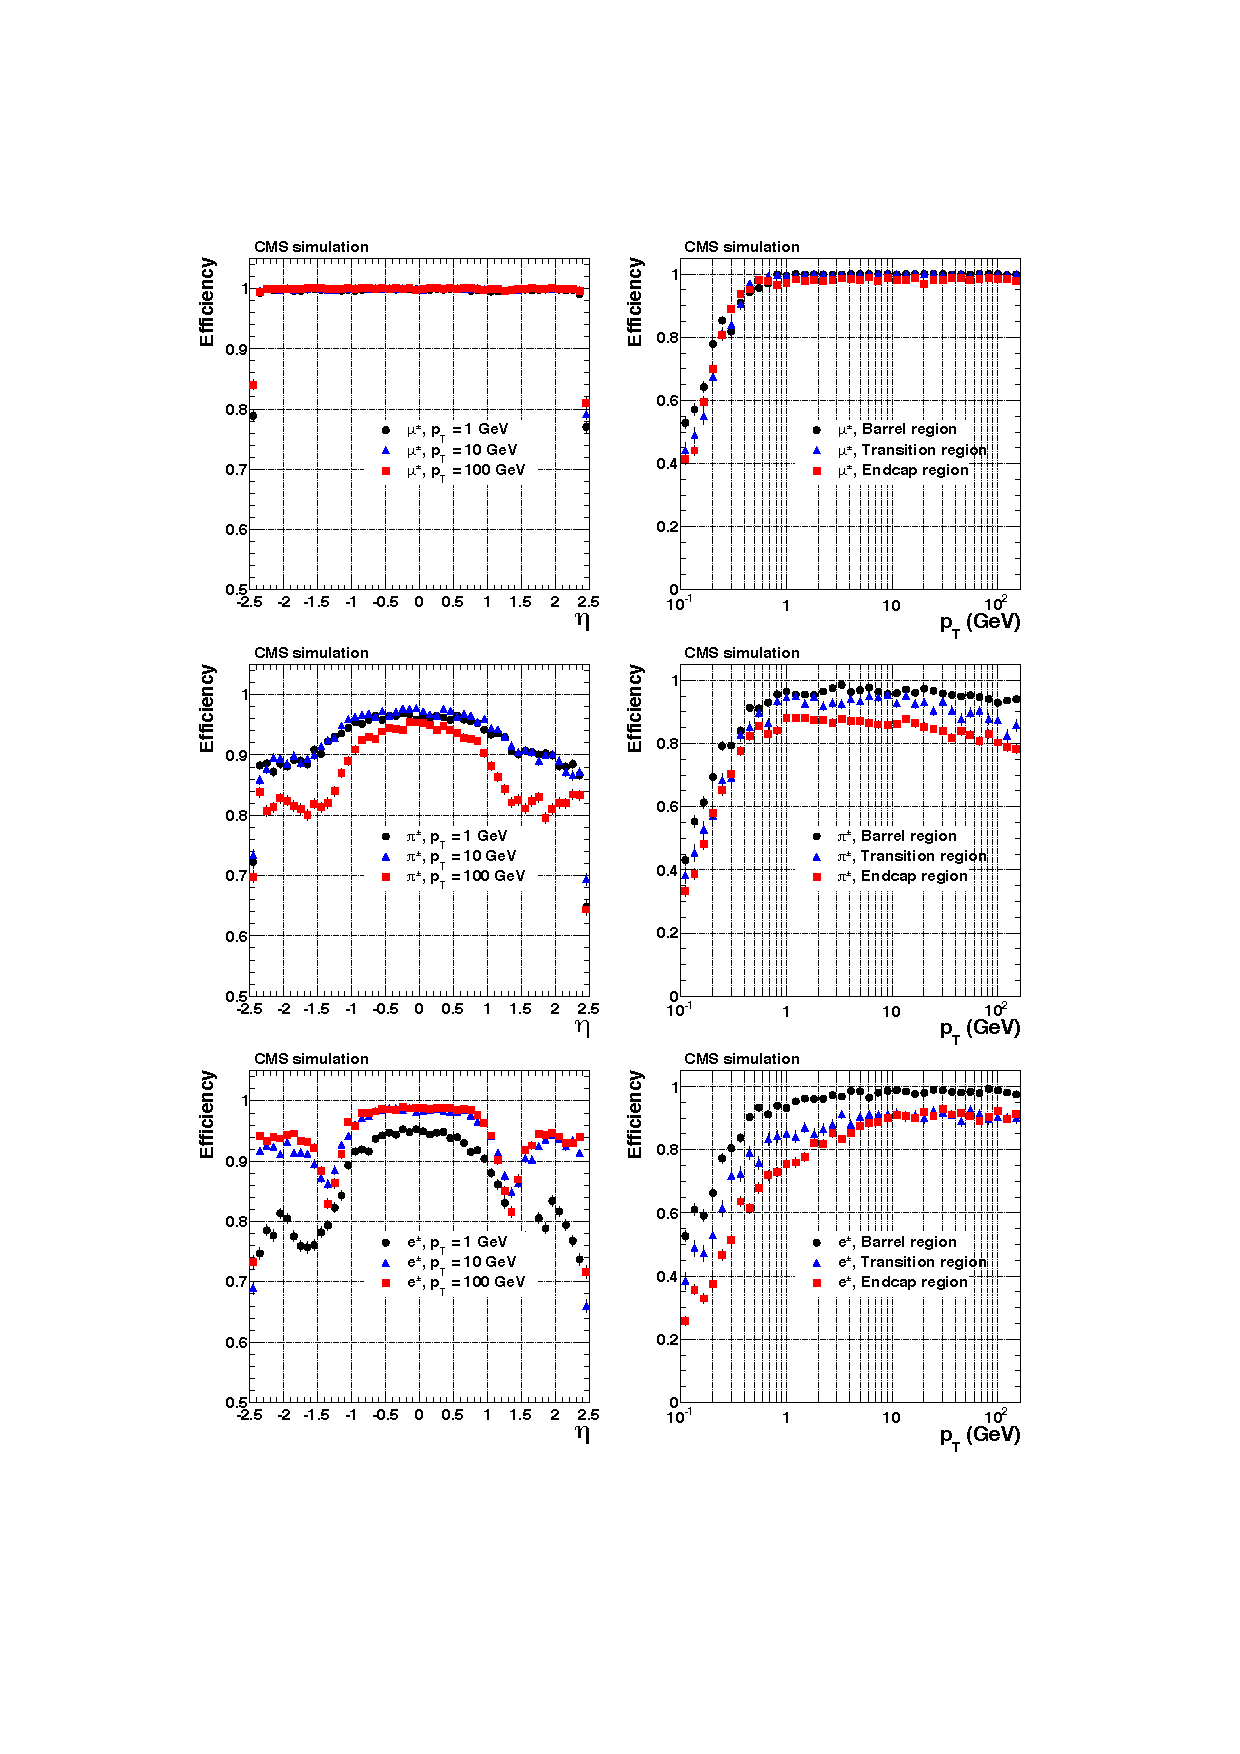
\includegraphics[width=0.8\linewidth]{figs/reconstruction/trackerPerformance} \end{center}
\caption{Efficiencies of track reconstruction for different charged
particles as a function of \pt and $\eta$. Muons are shown at the top,
pions in the middle and electrons at the bottom. The barrel,
transition and endcap regions are defined by the $\eta$ intervals of
0-0.9, 0.9-1.4 and 1.4-2.5 respectively.  For all the tracks
\emph{high-purity} quality requirements are made
\cite{Chatrchyan:2014fea}}
\label{fig:tracks_reco} \end{figure}

After charged particle tracks are reconstructed they can be used to
infer the positions of the different proton-proton collisions in the
event, known as interaction vertices. Tracks are required to originate
from a region that is compatible with the \LHC \emph{beamspot}, the area
in which the proton beams cross and collisions occur. The
$z$-coordinates of tracks at the closest point of approach to the
beamspot are taken as an input for the deterministic annealing
clustering algorithm \cite{726788:DA}. This finds the most probable
vertex positions and assigns each track to a vertex. The final
$x$,$y$,$z$ position of these vertices is then found using the
adaptive vertex fitter \cite{Waltenberger:2008zz}. This assigns the
most probable position of the vertex for the given set of input
tracks. Quality criteria are then applied to reject fake vertices,
they are chosen in such a way as to remain efficient for real vertices
that typically have a large number of tracks compatible with them.
Finally, the \emph{primary vertex} is determined as the vertex with
tracks that have the greatest scalar sum of \pt. Other vertices are
then initially attributed to \PU.  However, vertices that are
displaced from the initial proton collision are common signatures of
unstable particles that decay within the detector, such as
$b$-hadrons. These can be found in subsequent levels of
reconstruction.

The efficiency of finding the primary vertex as a function of the
number of tracks in a cluster can be seen in
Fig.~\ref{fig:vertex_reco}. The efficiency increases to close to
$>99\%$ for events with $\ge 3$ tracks. The vertex resolution reaches
$\sim10~\mu$m in $x,y$ and $\sim10~\mu$m in $z$ with $>40$
reconstructed tracks.

\begin{figure}
\begin{center}
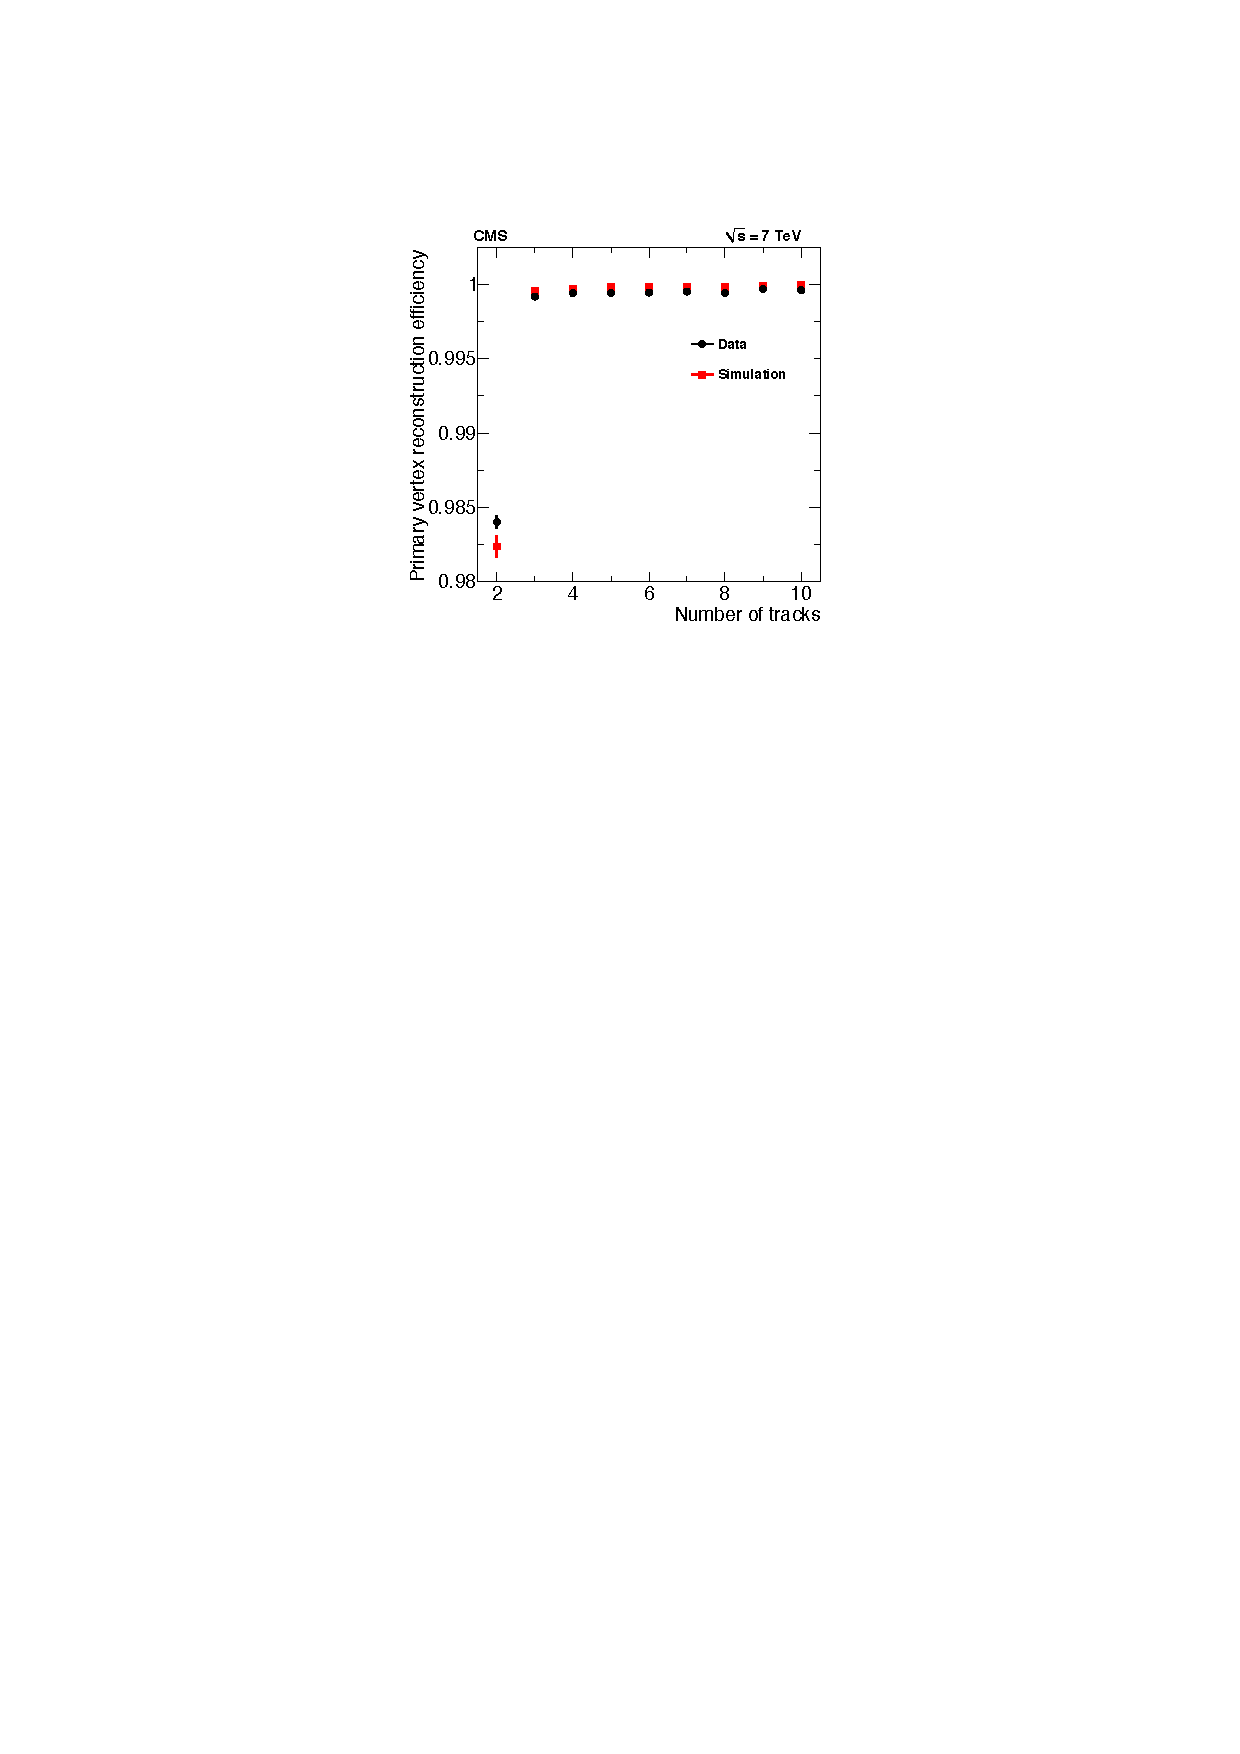
\includegraphics[width=0.5\linewidth]{figs/reconstruction/vertexPerformance} \end{center}
\caption{ The vertex reconstruction efficiency as a function of the
number of tracks originating from the vertex. Measured in data and
simulation for $\sqrt{s}=7~\tev$ proton collisions.
\cite{Chatrchyan:2014fea}}
\label{fig:vertex_reco} \end{figure}


\section{Particle flow}
\label{sec:pflow_reco}

Each of the subdetectors of \CMS provide complimentary information
about the different types of particles that pass through the detector.
This is exploited to identify the different types of particle with the
\PF algorithm
\cite{CMS-PAS-PFT-09-001,CMS-PAS-PFT-10-001,CMS-PAS-PFT-10-002}. As
\CMS has accurate momentum resolution in the tracker and a high
granularity \ECAL this algorithm allows both to augment the
measurement of objects in the \HCAL. This then allows calibrations
that are specific to both charged and neutral hadrons to be applied. 

The \PF algorithm searches for a set of individual particles that are
known as \PF \emph{candidates}. They are then classified as charged or
neutral hadrons, photons, muons or electrons. The set of \PF
candidates can then be utilised to calculate other event level
variables, such as for jet reconstruction described in
Sec.~\ref{sec:jets_reco}.
%Do i need to describe how clusters are made more?

The algorithm starts by taking the tracks, which are reconstructed as
in Sec.~\ref{sec:tracks_reco}, along with clusters of energy
in the calorimeters, which are reconstructed separately in the \ECAL and
\HCAL. Clusters are paired with tracks if the track trajectory is
compatible with the cluster position. These pairs are then used to
identify charged particles. Electrons and hadrons are typically
differentiated based on the proportion of energy they deposit in the
\ECAL or \HCAL. Electrons will deposit nearly all their energy in the
\ECAL whereas hadrons will deposit much more in the \HCAL. A similar
pairing between tracks and hits in the muon system is used to identify
muons. 

Neutral particles are then identified through calorimeter clusters
that do not have a compatible track associated to them. Photons, for
example, will leave a significant \ECAL deposit with no track, which
would be present for electrons. Similarly, neutral hadrons will leave
significant deposits in the \HCAL with no associated track.

\section{Electrons and photons}
\label{sec:electrons_reco}

Both electrons and photons interact with the \ECAL in a similar way.
The reconstruction techniques used for both are therefore very similar, with
the main difference being the lack of track in photon reconstruction.
As electrons interact with the tracker, they lose on average $33\%$ of
their energy before reaching the \ECAL \cite{1748-0221-10-06-P06005}.
Most of this energy loss occurs through bremsstrahlung, which has a
non-Gaussian loss distribution. As the Kalman filter that is used in
track reconstruction assumes Gaussian energy losses, another specialist
track reconstruction for electrons is employed, known as the Gaussian
Sum Filter algorithm \cite{Adam:815410}. To maintain a good energy
resolution, the photons that are produced during bremsstrahlung must
also be properly associated to the electron when clustering in the
calorimeter. As the electrons bend in the magnetic field but the
photons they emit do not, the calorimeter clusters are allowed to
extend along the azimuthal direction. These rectangular \ECAL windows
are know as \emph{superclusters}.

To form the superclusters in the barrel the \emph{hybrid} clustering
algorithm is used. A single seed crystal with a local maximum
transverse energy $E_T>1~\gev$ is identified and a rectangular
configuration of $3\times 1$ or $5\times 1$ crystals in $\eta$-$\phi$
is formed around it. The algorithm then looks in the $\phi$ region
adjacent to this rectangle up to $\Delta\phi\pm 0.3$.
Additional rectangular regions that have $E_T>100$~MeV are kept and
grouped to form the supercluster. In the endcaps the \emph{multi $5\times
5$} algorithm is used instead, which aggregates $5\times 5$ arrays of
crystals within $\Delta\eta<0.07$ and $\Delta\phi<0.3$ of the seed.

Electrons are identified through a supercluster matched to a track, or
photons are identified through an unmatched supercluster. After
this, additional selection criteria are applied to suppress
backgrounds. The major backgrounds come from misreconstructed hadronic
jets or semi-leptonic decays of heavy quarks. To suppress them cuts
are made on the ratio of energy deposits in the \HCAL and the \ECAL, the
difference in direction between the track and supercluster (in the
case of electrons) and the width of the cluster, which is larger for
hadrons.

\section{Muons}
\label{sec:muons_reco}

Unlike electrons and photons, muons are minimally ionising so do not
deposit much of their energy in the tracker or calorimeters
\cite{Chatrchyan:2008aa}. Muon reconstruction therefore
uses a combination of tracks and hits in the muon system. To maintain
efficiencies across a wide range of muon energies, two algorithms are
utilised \cite{1748-0221-7-10-P10002}. The \emph{global} muon algorithm
functions in the same way as the \PF algorithm, mentioned in
Sec.~\ref{sec:pflow_reco}. To maintain efficiency for low energy muons
that have a lower probability of traversing the entire muon system
the \emph{tracker} muon algorithm is additionally used.

The global muon algorithm starts with hits in each layer of the muon
system that give an initial estimate of the position, energy and
direction of candidate muons. It then searches for tracks in the inner
detector that are compatible with this candidate. If this is the case,
the track is extrapolated to the hits in the muon system using a
Kalman filter, similar to the way tracks are reconstructed in
Sec.~\ref{sec:tracks_reco}. 

The tracker muon algorithm starts with tracks with $\pt>0.5~\gev$ and
extrapolates them into the muon system, again with a Kalman filter. If
any of these tracks can be matched to at least one muon chamber hit it
is considered to be a muon. For muons with $\pT<200~\gev$ the tracker
provides the highest resolution energy measurement, while the muon
system provides a better resolution for the straighter, higher \pT,
tracks.

To reduce the background from hadrons that have punched through the
\HCAL or muons that do not originate from the primary vertex, such as
those from cosmic
rays, a series of selections are applied to the reconstructed
muon candidates. These include a quality requirement on the fit of the
tracks, a minimum number of hits in the muon systems and a track
compatible with originating from the beamspot. A different set of
criteria can be applied to trade off the efficiency and fake rate of
the muons. After an application of a \emph{tight} set of criteria, the
efficiency of muons with $\pT>10~\gev$ is measured to be $>96\%$,
shown in Fig.~\ref{fig:muonEff}.

\begin{figure}
\begin{center}
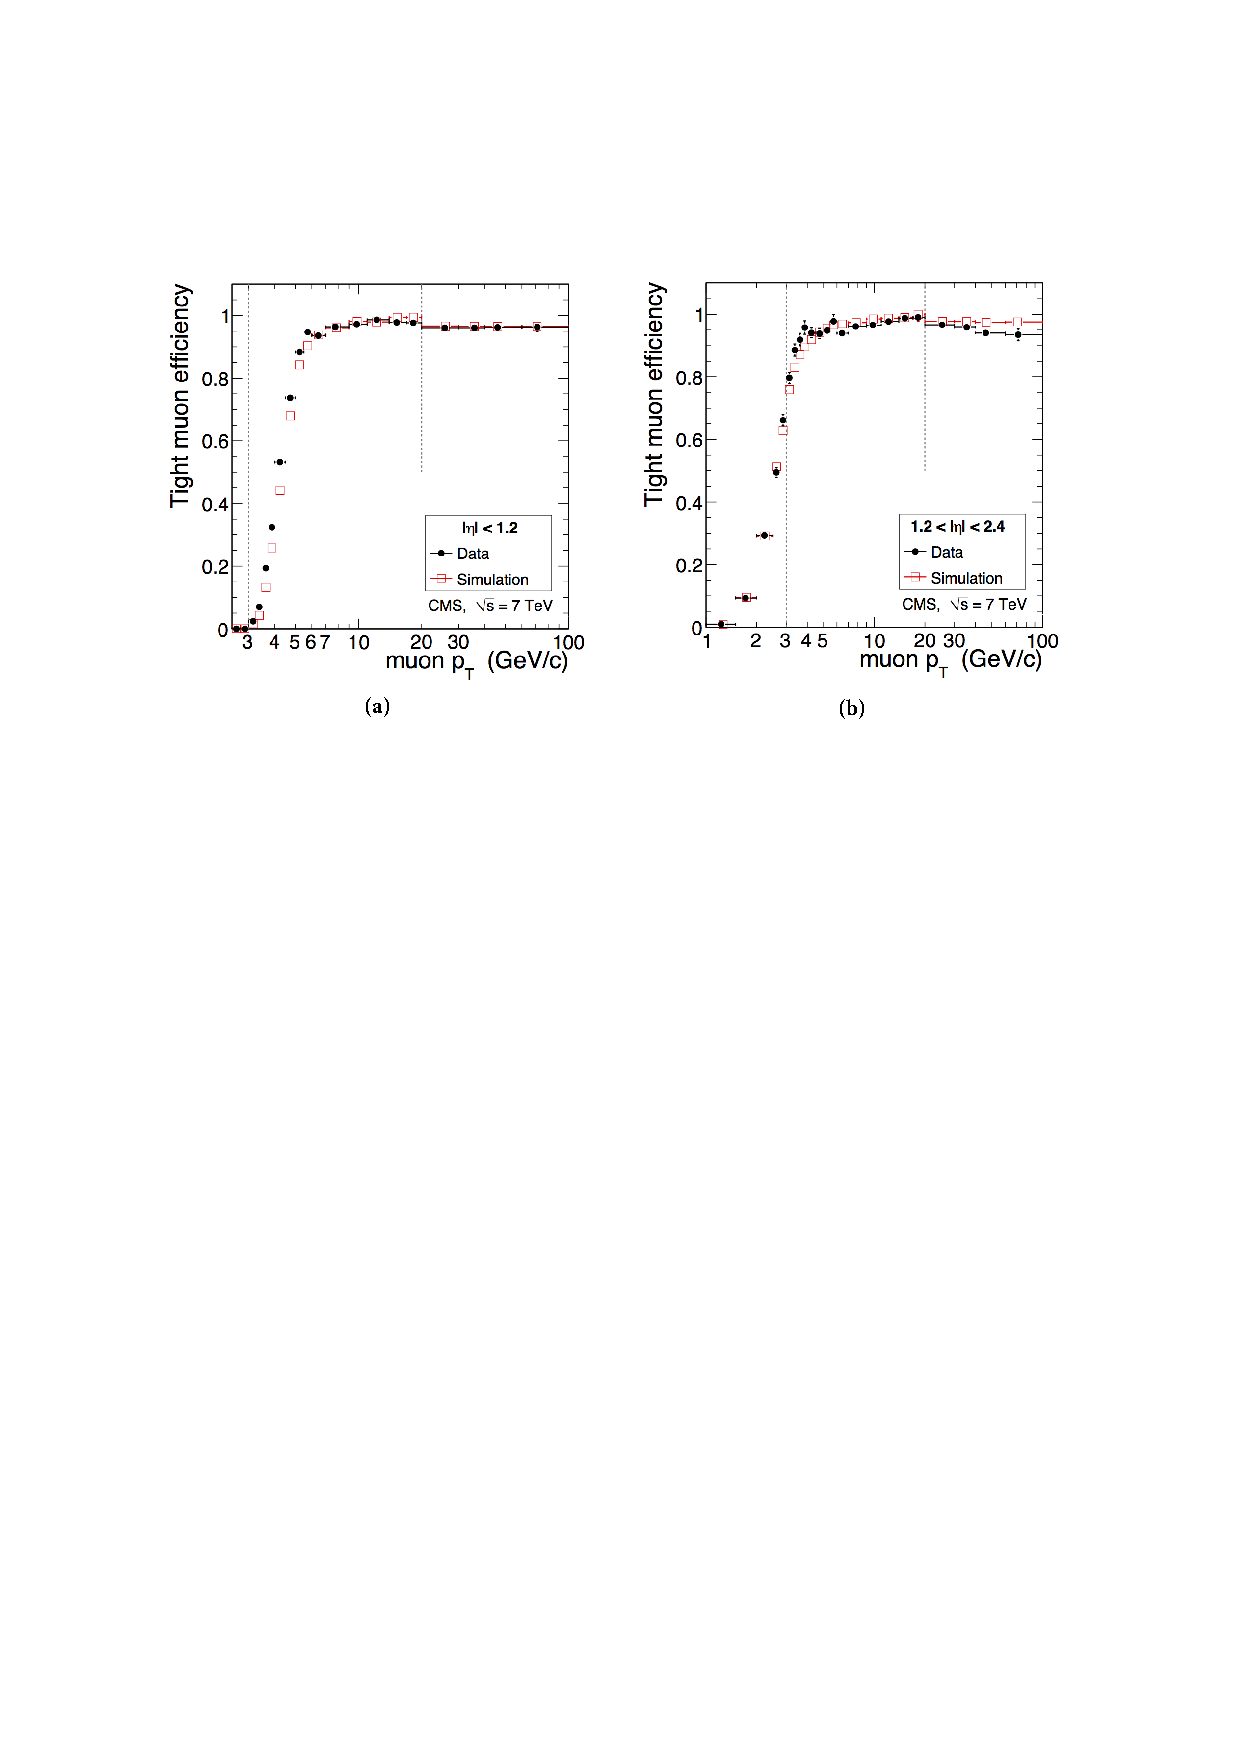
\includegraphics[width=0.9\linewidth]{figs/reconstruction/muonEff} \end{center}
\caption{ The tight muon reconstruction efficiency as a function of the
\pt of the muon in $\sqrt{s}=7~\tev$ proton collisions. The efficiency
is measured separately in the barrel (a) and endcap (b) regions.
\cite{1748-0221-7-10-P10002}}
\label{fig:muonEff} \end{figure}

\section{Jets}
\label{sec:jets_reco}

As there is a very high probability that proton collisions will
produce quarks and gluons, identifying and measuring them is a crucial part of
object reconstruction in \CMS. This is particularly relevant when
searching for strongly produced \SUSY particles as they typically
decay via hadrons to the \LSP, as described in
Chapter~\ref{chap:theory}. Due to the nature of the strong force,
high $\pT$ quarks and gluons undergo immediate hadronisation. The
result of this is a collimated shower of, predominantly hadronic,
particles. To reconstruct the quarks and gluons produced in
an event these collimated showers of particles are clustered and
reconstructed as \emph{jets} \cite{Salam2010}.

\subsection{The anti-$k_T$ clustering algorithm}

When determining the clustering algorithm to be used, the theoretical
behaviour of hadronisation must be taken into account
\cite{Salam2010}. Specifically, jets can undergo soft gluon radiation
of arbitrarily low energy gluons with a high probability.
Similarly, a gluon can split into two, almost collinear, gluons that share its energy.
The final result of the clustering algorithm cannot not depend
on either of these things happening. It must be both
\emph{infrared safe} and \emph{collinear safe}. The jet algorithms used in \CMS are
typically some form of a \emph{sequential recombination algorithm} that
fulfills the above criteria. After defining a \emph{distance}
between all pairs of particles in the event, $d_{ij}$, and a distance
from each particle to the beamline, $d_{iB}$, the algorithm undertakes
the following steps:
\begin{itemize}
\item{Calculate $d_{ij}$ for all pairs of particles in the event and
$d_{iB}$ for each particle.}
\item{If a value of $d_{ij}$ is smallest, combine the pair of particles
with this distance into a single new particle and start again.}
\item{If a value of $d_{iB}$ is smallest remove this particle from the
list of particles, classify it as a cluster and start again.}
\item{Stop when there are no more particles remaining.}
\end{itemize}
For the sequential recombination algorithms used by \CMS the distance
parameters used are defined as:
\begin{equation} \label{eq:antiktdij}
d_{ij} = \textrm{min}(p_{Ti}^{2k},p_{Tj}^{2k})\frac{\Delta R_{ij}^2}{R^2} ,~~~~d_{iB} = p_{Ti}^{2k}
\end{equation} 
for particles $i$ and $j$ where $k=-1,0,1$, $\Delta R$
is the separation in the $\eta$-$\phi$ plane and $R$ is a fixed
parameter that sets the jet size. The most commonly used of the \CMS
algorithms has $k=-1$ and is known as the \emph{anti-$k_T$} algorithm
\cite{1126-6708-2008-04-063}. The anti-$k_T$ algorithm tends to
cluster circular jets built around the hardest particles in a
particular event. An area of $R=0.4$ is often
chosen as it contains the hadronic showers of most quarks and gluons
while remaining insensitive to contamination from \PU.

\subsection{Jet identification}

For the results presented in this thesis the \textsc{FastJet}
\cite{Cacciari2012} package is used to cluster the \PF candidates,
that are described in Sec.~\ref{sec:pflow_reco}. The
anti-$k_T$ algorithm is used with $R=0.4$. The \PF candidates
add information from the tracker when
calculating the momentum contribution to each jet from charged
particles. As jets typically consist of 65\% charged hadrons, 25\%
photons and 10\% neutrals, this gives a significant improvement over
clustering the calorimeter deposits on their own. 

To reject fake jets from background sources or detector noise,
additional selection is applied to jet candidates. The \emph{loose} set of
criteria for jets provides an 84\% suppression of fake jets while
maintaining a $>99\%$ efficiency for real jets. It requires at least
two \PF candidates; $<99\%$ of the jet to come from only hadrons,
photons or electrons; and at least one charged track.

\subsection{Jet energy corrections}
\label{sec:reco_jec}

Due to the imperfect resolution of the \CMS detector the initial
measured transverse momentum, $p_T^{raw}$, of a jet does not
necessarily match the energy of the particle that initiated the jet.
The difference between the \emph{raw} \pT and the \emph{true} \pT typically
depends on the \pT of the jet and its position in the detector, along
with components of the jet that are measured by different
subdetectors. To correct the raw \pT of the jet, a correction is
applied with the functional form
\cite{1748-0221-6-11-P11002}:
\begin{equation}
p_T^{cor}=C^{Off}(p_T^{raw},\rho,A_j)\cdot C^{Rel}(\eta)\cdot
C^{Abs}(p_T^{Rel})\cdot C^{Res}(p_T^{Abs})\cdot p_T^{raw}.
\end{equation}

The first step is the offset calibration, $C^{Off}$, which performs a correction
that removes the effect of other jets originating from \PU in the jet
cone. Initially, the contribution made by charged particles that do
not originate from the primary vertex is removed. This process is
known as \ac{CHS}. The remaining contribution from neutral \PU
particles is corrected using jet area subtraction
\cite{Cacciari:2007fd}. In this case the jet area, $A_j$ is multiplied
by the average pileup energy density, \rho. The value of \rho is
determined from the energy density of \PF candidates across the entire
detector.  Next, a relative correction, $C^{Rel}$, is applied as a
function of the \eta of the jet. This compensates for the differing
response of different parts of the detector across different
pseudorapidity ranges. An absolute correction, $C^{Abs}$ is then
applied on the output of the first two calibration steps, $p_T^{Rel}$.
This correction is designed to correct the dependence of the jet \pT
on the magnitude of the measured \pT. These two corrections are
calculated using information taken from both simulation and data. %Zbalance and dijet balance.
The final correction, $C^{Res}$, is applied only to data and not
simulation. This is designed to correct the residual differences in
the \pT and $\eta$ response between the data and simulation. The
magnitude of the corrections as a function of $\eta$ for two
representative values of \pT can be seen on Fig.~\ref{fig:jec}.

%put in performance figure?

\begin{figure}
\begin{center}
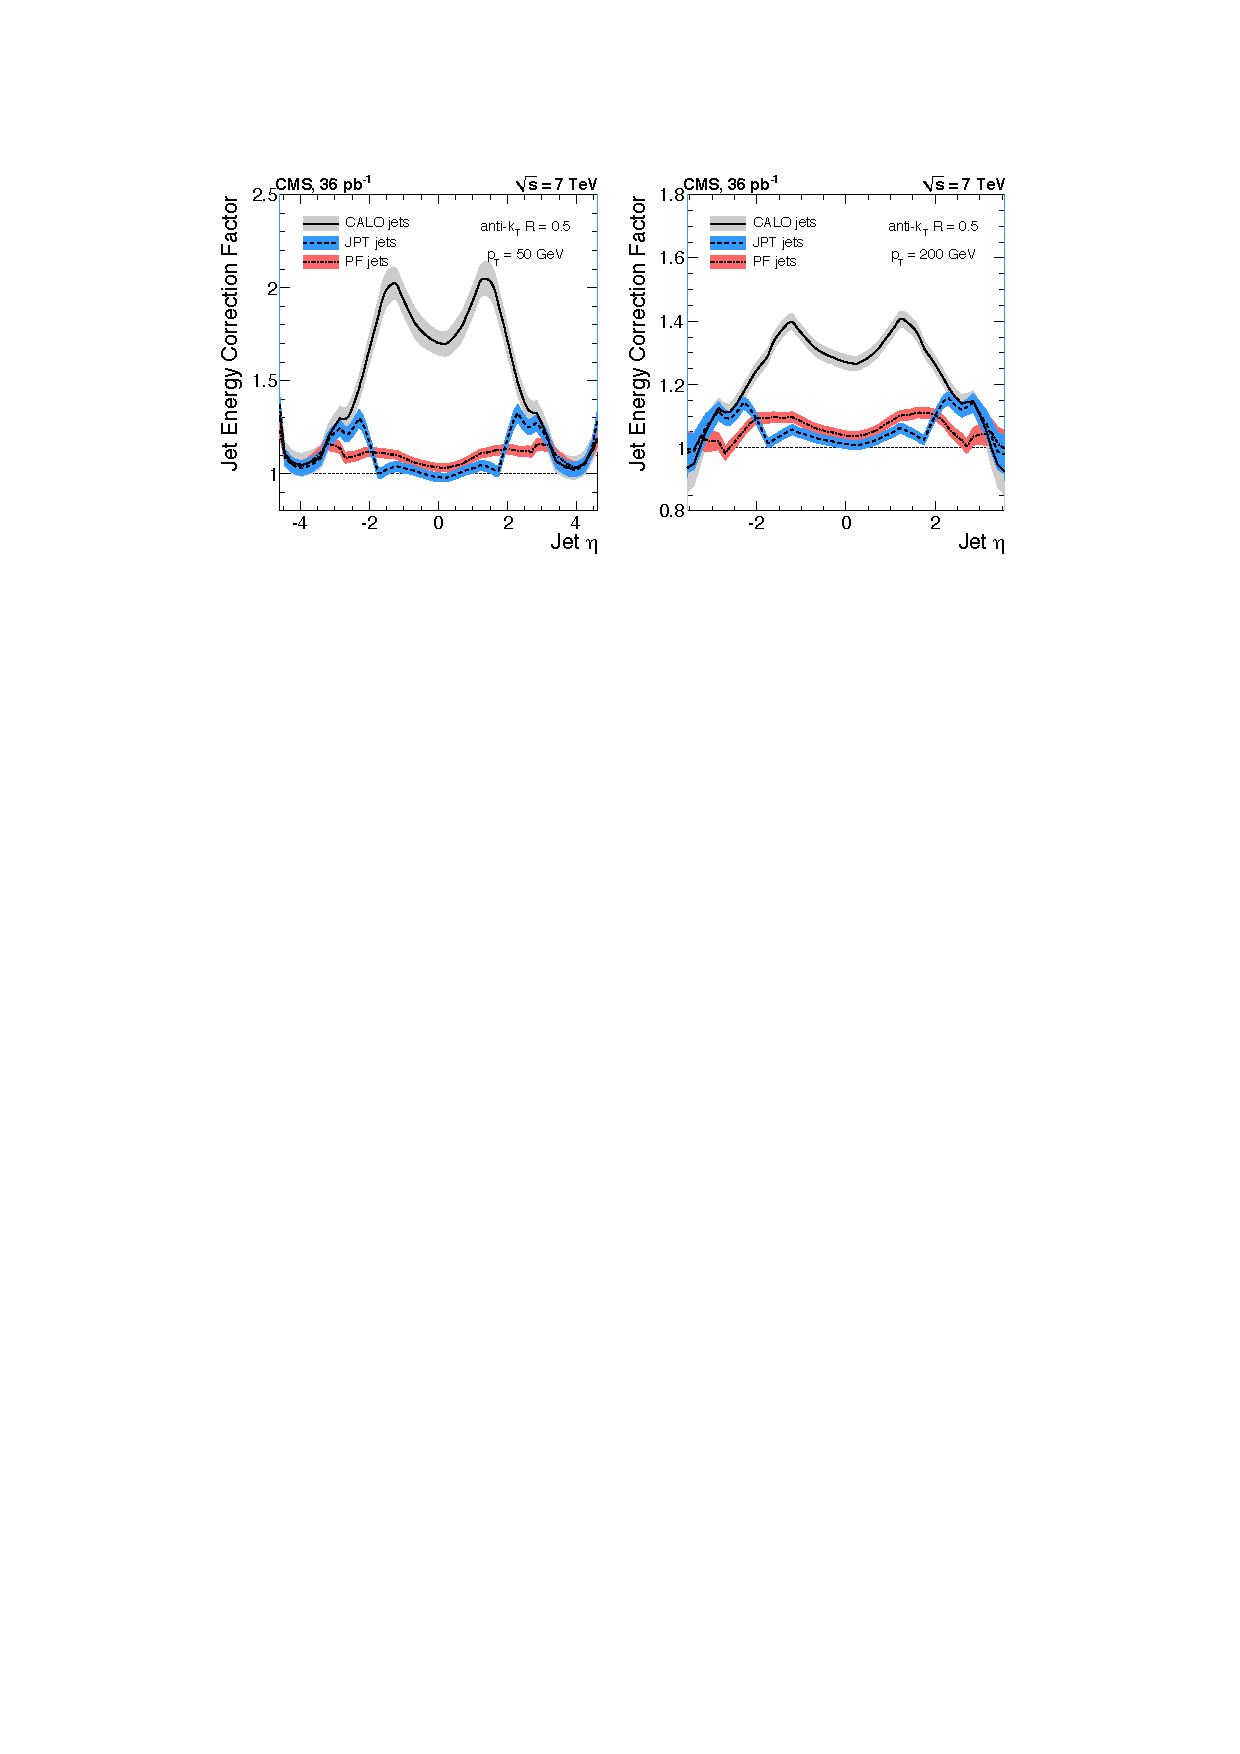
\includegraphics[width=0.9\linewidth]{figs/reconstruction/jec} \end{center}
\caption{The jet energy correction factors and their corresponding
uncertainty as a function of jet \eta
for jets with $\pT=50~\gev$ (left) and jets with $\pT=200~\gev$
(right) for different types of jet reconstruction. The correction for jets
reconstructed with \PF candidates is shown in the red line, the CALO
label indicates jets reconstructed purely with calorimeter deposits
and no tracker information \cite{1748-0221-6-11-P11002}}
\label{fig:jec} \end{figure}

\subsection{Tagging $b$-jets}

The $b$-quark is of particular interest when searching for
indications of new physics. The production of these
quarks is relatively rare in \SM interactions and often
indicate the presence of a top quark that has decayed to a
$b$. In a wide range of \SUSY models the decay via top quarks is
favoured over other, lighter quarks. It is therefore very advantageous
to have a way of identifying jets as originating from $b$-quarks,
known as \emph{$b$-tagging}.

As $b$-hadrons have a relatively long lifetime, $\tau\sim 1.5$~ps
\cite{PhysRevD.86.010001}, they typically travel $c\tau\sim 450~\mu$m
from the primary vertex before decaying. The \CMS tracker has a
spatial resolution $\sim 30~\mu$m for $\sim 5~\gev$ tracks, which
means the displaced vertex created by the $\sim 5~\gev$ mass $b$-quarks
can be resolved. This is exploited by the \ac{CSVv2} algorithm used
for $b$-tagging in Run~2 \cite{CMS-PAS-BTV-15-001}. This algorithm
uses a neural net with detector inputs, including vertices identified
by the tracker that are displaced from the primary vertex and
associated to the jet and information about the tracks originating
from this vertex.

As with the other physics object definitions in this chapter,
different selection criteria can be chosen to trade-off the mistag
rate and efficiencies for $b$-tagging. For each working point a
different discrete cut on
the \ac{CSVv2} discriminator is chosen, its distribution is shown in
Fig.~\ref{fig:bTag}. A \emph{medium} working point cut of 0.8 corresponds to
a tagging efficiency of $\sim 69\%$ and a mistag rate of $\sim 1\%$
\cite{CMS-PAS-BTV-15-001}. 

\begin{figure}
\begin{center}
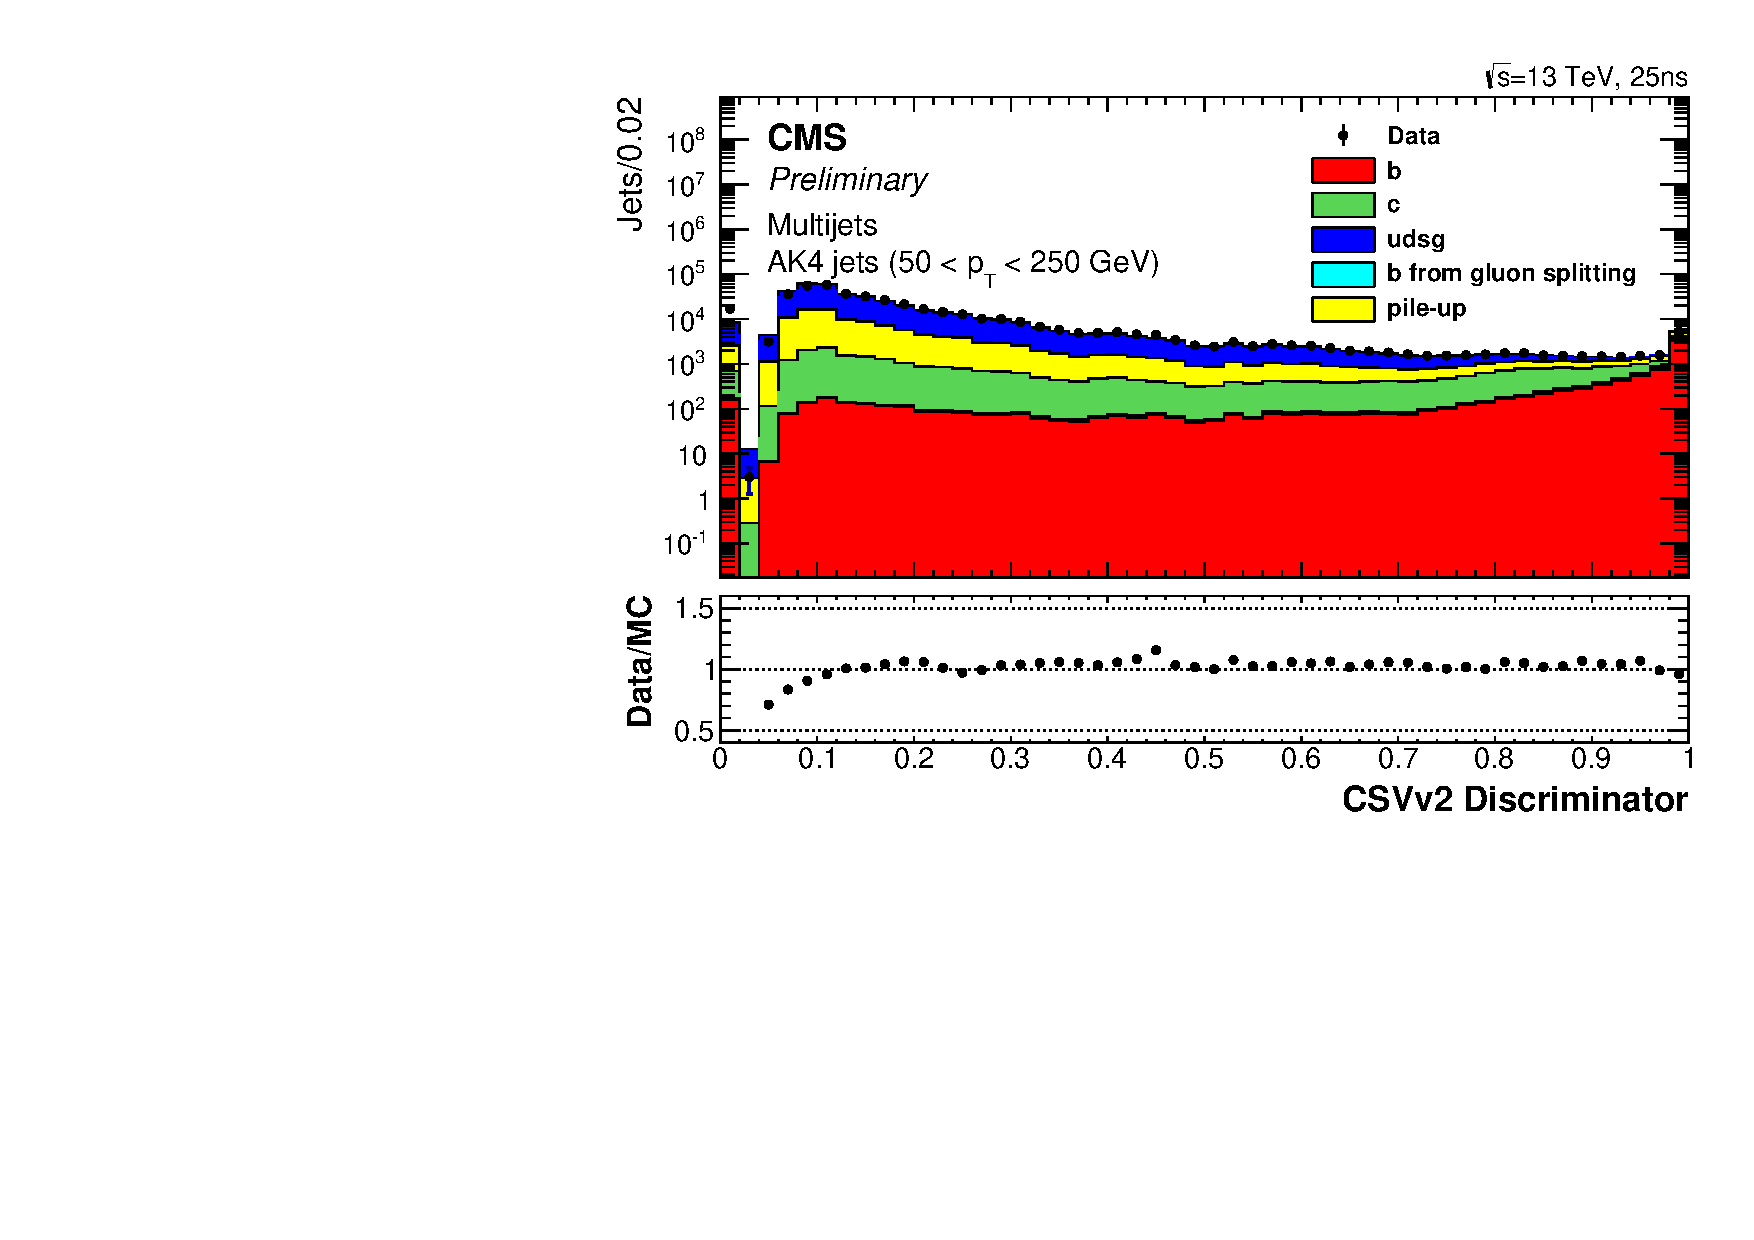
\includegraphics[width=0.7\linewidth]{figs/reconstruction/bTag} \end{center}
\caption{ The distribution of the discriminator \ac{CSVv2} algorithm
for $b$-tagging in multijet events. Tagged jets are clustered with the
anti-$k_T$ algorithm with $R=0.4$ and span $50<\pT<250~\gev$. A
working point is chosen to trade off b-tagging efficiency for mistag
rate by making a cut on the discriminator \cite{CMS-PAS-BTV-15-001}.}
\label{fig:bTag} \end{figure}

\section{Isolation and jet cross-cleaning}

It is often important to differentiate \emph{prompt} leptons produced
directly in the primary vertex from those that are the result of decays
of other particles, such as those in hadronic jets. To do this an
\emph{isolation} variable, $I^{\textrm{rel}}$, is defined for each
lepton. To construct it the \pT of the \PF candidates within a cone
around the lepton are summed and the estimated neutral-charged
contribution of \PU within that cone is subtracted. This is then
divided by the \pT of the lepton in question, $\pT^l$. In the case
that the lepton is part of a jet $I^{\textrm{rel}}$ will have a large
value, this will not typically be the case if it is prompt.

In the work presented in this thesis, two variants of cone size are
used. In the standard case, denoted $I^{\textrm{rel}}$, a cone size
of $\Delta R=0.3$ is used. To maintain acceptance to leptons produced
in the decays of boosted objects, such as top-quarks, a
\emph{mini-isolation} can be defined that has a variable cone that
depends on the \pT of the object. A value of $\Delta R=0.2$ is chosen
for $\pT^l<50~\gev$, but this is scaled down to a minimum $\Delta
R=0.05$ for $\pT^l>200~\gev$.

The contribution from \PU is typically estimated in two different
ways. For \emph{effective-area} correction the average \PU energy
density of neutral particles, $\rho^{\textrm{neutral}}$, is multiplied
by the area of the isolation cone, similar to the \PU correction
carried out in jets as described in Sec.~\ref{sec:reco_jec}. For
\emph{$\Delta\beta$} correction the energy of neutral particles is
estimated as half the energy from charged particles that originate
from \PU vertices in the cone. This ratio of charged to neutral
particles is determined from simulation. % reference??

To avoid isolated leptons being classified as jets, a
\emph{cross-cleaning} is performed on the result of the jet clustering.
In this case all jets that are within $\Delta R=0.4$ of an isolated
lepton are removed from the event.

\section{Missing transverse energy (\met) and energy sums}
\label{sec:met_reco}

Weakly interacting particles, such as neutrinos or neutralinos, will
pass through all components of the \CMS detector. Their production can
therefore only be inferred from the imbalance of momentum in the decay
products of a proton collision that can be observed by \CMS. To
measure the magnitude and direction of the missing momentum the
missing transverse energy variable, \met, is defined as the negative
vector sum of the momentum, $\vec{p}_T$, of all the particles in an
event:
\begin{equation}
\met = -\sum{\vec{p}_T}.
\end{equation}
This is reconstructed taking the \PF candidates up to $|\eta|<5$ as
input \cite{1748-0221-10-02-P02006}. 

A correction is applied to \met based on the jet energy correction
described in Sec.~\ref{sec:reco_jec}. This is known as the \emph{Type-I}
correction and applies the jet energy correction to the \PF candidates that are
clustered into jets. This method takes jets with $\pT>15~\gev$ and
helps to signficantly improve the \met resolution.

It is also advantageous to define other energy sums that take only
jets as input, which are typically better understood and calibrated
than each unclustered \PF candidate. To gain a measure of the scale of
hadronic energy in an event the \HT variable is defined as the scalar
sum of jet momenta, $\pT^{\textrm{jet}}$. To gain an alternative
measure of the missing energy the negative vector sum of jet momenta,
$\vec{\pT}^{\textrm{jet}}$, denoted  \MHT is defined.
\begin{equation}
\HT = \sum{\pT^{\textrm{jet}}},~~~~\MHT =
-\sum{\vec{\pT}^{\textrm{jet}}}.
\end{equation}

\section{Monte Carlo (MC) simulation}
\label{sec:mc_reco}

A major part of understanding the data collected by \CMS involves the
use of simulated events for different types of \SM and \BSM processes.
With a good simulation, it is possible to classify the events observed
in data as demonstrating particular physical processes that are
predicted by theory. The simulation of proton collisions is
particularly challenging, as it requires an accurate modelling of a
wide range of \SM phenomena as well as a very good understanding of
the \CMS detector. The simulation is split up into a series of
stages that split up the theoretical simulation and detector modelling
\cite{Buckley:2011ms}. 

In the first stage, the hard scattering of the colliding constituents,
\emph{partons} of the incoming protons through electroweak or QCD
interactions is modelled. The fraction of the proton momentum carried
by each parton is sampled from a \ac{PDF}. This modelling involves a
calculation with perturbation theory to a fixed order, typically \LO
or \NLO, with a dedicated \MC generator such as \textsc{MadGraph}
\cite{Alwall:2011uj} or \textsc{Pythia} \cite{Sjostrand:2007gs}.

In the next stage an iterative process of \emph{parton showering} is
carried out. Simulated QCD radiation from the hard scatter decay
products is carried out until the particles in the shower reach the
QCD cut-off scale, $\Lambda_{\textrm{QCD}}\sim 1~\gev$, where
perturbation theory breaks down. After the parton showering the
remaining particles undergo hadronisation where colourless hadrons are
formed and allowed to decay, resulting in \emph{generator-level}
particles with well defined four-momenta. The hadronisation is carried
out with MC generators such as \textsc{Pythia} \cite{Sjostrand:2007gs}
and \textsc{Herwig} \cite{Bahr:2008pv} that each use different
techniques to carry the connection of the colour-flow from the initial
state to final state particles. Remaining unstable particles have
their decays simulated with dedicated \MC algorithms.

The output of the hadronisation stage is then passed through a
simulation of \CMS with software such as \textsc{Geant4}
\cite{Agostinelli:2002hh}. The individual components and their
responses are faithfully reproduced to output a simulated event that
is comparable to one measured in real proton collisions. The standard
reconstruction, such as that described in this chapter, can then be
performed.

Finally, the \PU must be simulated in \MC. A large sample of minimum
bias, typically soft, QCD events are simulated. Individual events from
this sample are taken and overlaid on the simulated event of interest
to imitate the effects of \PU. The effects of \ac{OOTPU} are also
taken into account by simulating other minimum bias \MC events within
a $12$ bunch crossing window.


  \chapter{The Level-1 trigger upgrade jet algorithm}
\label{chap:l1trig}

\section{The Calorimeter Trigger upgrade for Run~2}
\label{sec:trigUpgrade}

With the advent of Run~2 of the \LHC, the demands placed on the \CMS
trigger greatly increased. After a long period of shutdown (known as
\ac{LS1}) the energy
of proton collisions was increased to $13~\tev$ and the bunch crossing
rate decreased to 25~ns. With this configuration the design luminosity
of $10^{34}$cm$^{-2}$s$^{-1}$ can be reached with an average \PU of
around 25 events per bunch crossing. However, the potential luminosity
of the \LHC after the \ac{LS1} upgrade exceeds the original design
value, allowing a \PU of up to 40 simultaneous collisions. The
original Level-1 trigger was not designed to deal with this amount of
\PU. The presence of extra collisions in each event results in a
general increase in the average energy deposited in the calorimeters
of the detector. This extra energy smears out the measurement of
energy deposited by particles from the hard scatter, reducing the
resolution with which it is measured. This acts to increase the rate
at which the trigger accepts events and decrease the accuracy with
which it identifies interesting events. As this rate is limited by the
readout capability, a trigger that is not upgraded will have a reduced
efficiency of acceptance of interesting physics events.  It is
therefore very advantageous to upgrade the Level-1 trigger in a way
that allows it to deal with the extra \PU \cite{Tapper:1556311}.

Along with maintaining a low output rate for a high efficiency,
another key consideration for the Level-1 trigger is the time taken
for
the algorithms to run on the boards that carry out the trigger
processing, their \emph{latency}. This must be kept low to ensure that
every bunch
crossing is analysed in as much detail as possible. To be able to
carry out this sort of processing, the Level-1 trigger makes use of custom
\FPGA boards, as described in Sec.~\ref{sec:triggers}. The complexity
and structure of the trigger algorithms is limited to ensure
they can run quickly enough on the \FPGA boards. An upgrade to the
trigger hardware therefore allows more sophisticated algorithms to be
carried out, while still being able to process every bunch crossing.

The amount of calorimeter information that can be processed by a
single \FPGA is also limited by its input and output capacity. To pass
the full calorimeter data from a single bunch crossing through an
\FPGA in the Level-1 trigger it takes the equivalent of $\sim10$ bunch
crossings of time. In Run~1 of the \LHC, the calculations for
triggering on the calorimeters were performed with the \GCT
\cite{Khachatryan:2016bia}. The \GCT dealt with this delay by
processing different sections of the calorimeter in separate boards,
necessitating duplication of information at the detector section
boundaries. However, by time multiplexing the calorimeter data, it is
possible to have individual \FPGA boards that each process one bunch
crossing with minimal information duplication. To achieve this, 10
\FPGA boards are utilised in a round-robin configuration. The data
collected from the first bunch crossing is processed by one board, the
data from the second bunch crossing by another board and so on. Each
bunch crossing is processed by another board until the first board has
finished and can subsequently process the next available bunch
crossing. This would not be possible without the timing information
provided by time multiplexing the data. As well as increasing the
total possible information bandwidth, this allows greater flexibility
in the algorithms used as each \FPGA has access to the full event
information \cite{1748-0221-9-10-C10034,1748-0221-7-01-C01060}. The
upgrade architecture of the Level-1 trigger is therefore that of a
\TMT, a representation of the difference between this architecture and
that of the \ac{GCT} can be seen in Fig.~\ref{fig:tmt}. The hardware
is also upgraded, exploiting the recent technological improvement in
the performance of \FPGA processors and high-speed optical links
\cite{tp}.

\begin{figure}
  \centering
  \subfloat[Run~1 trigger architecture.]{
    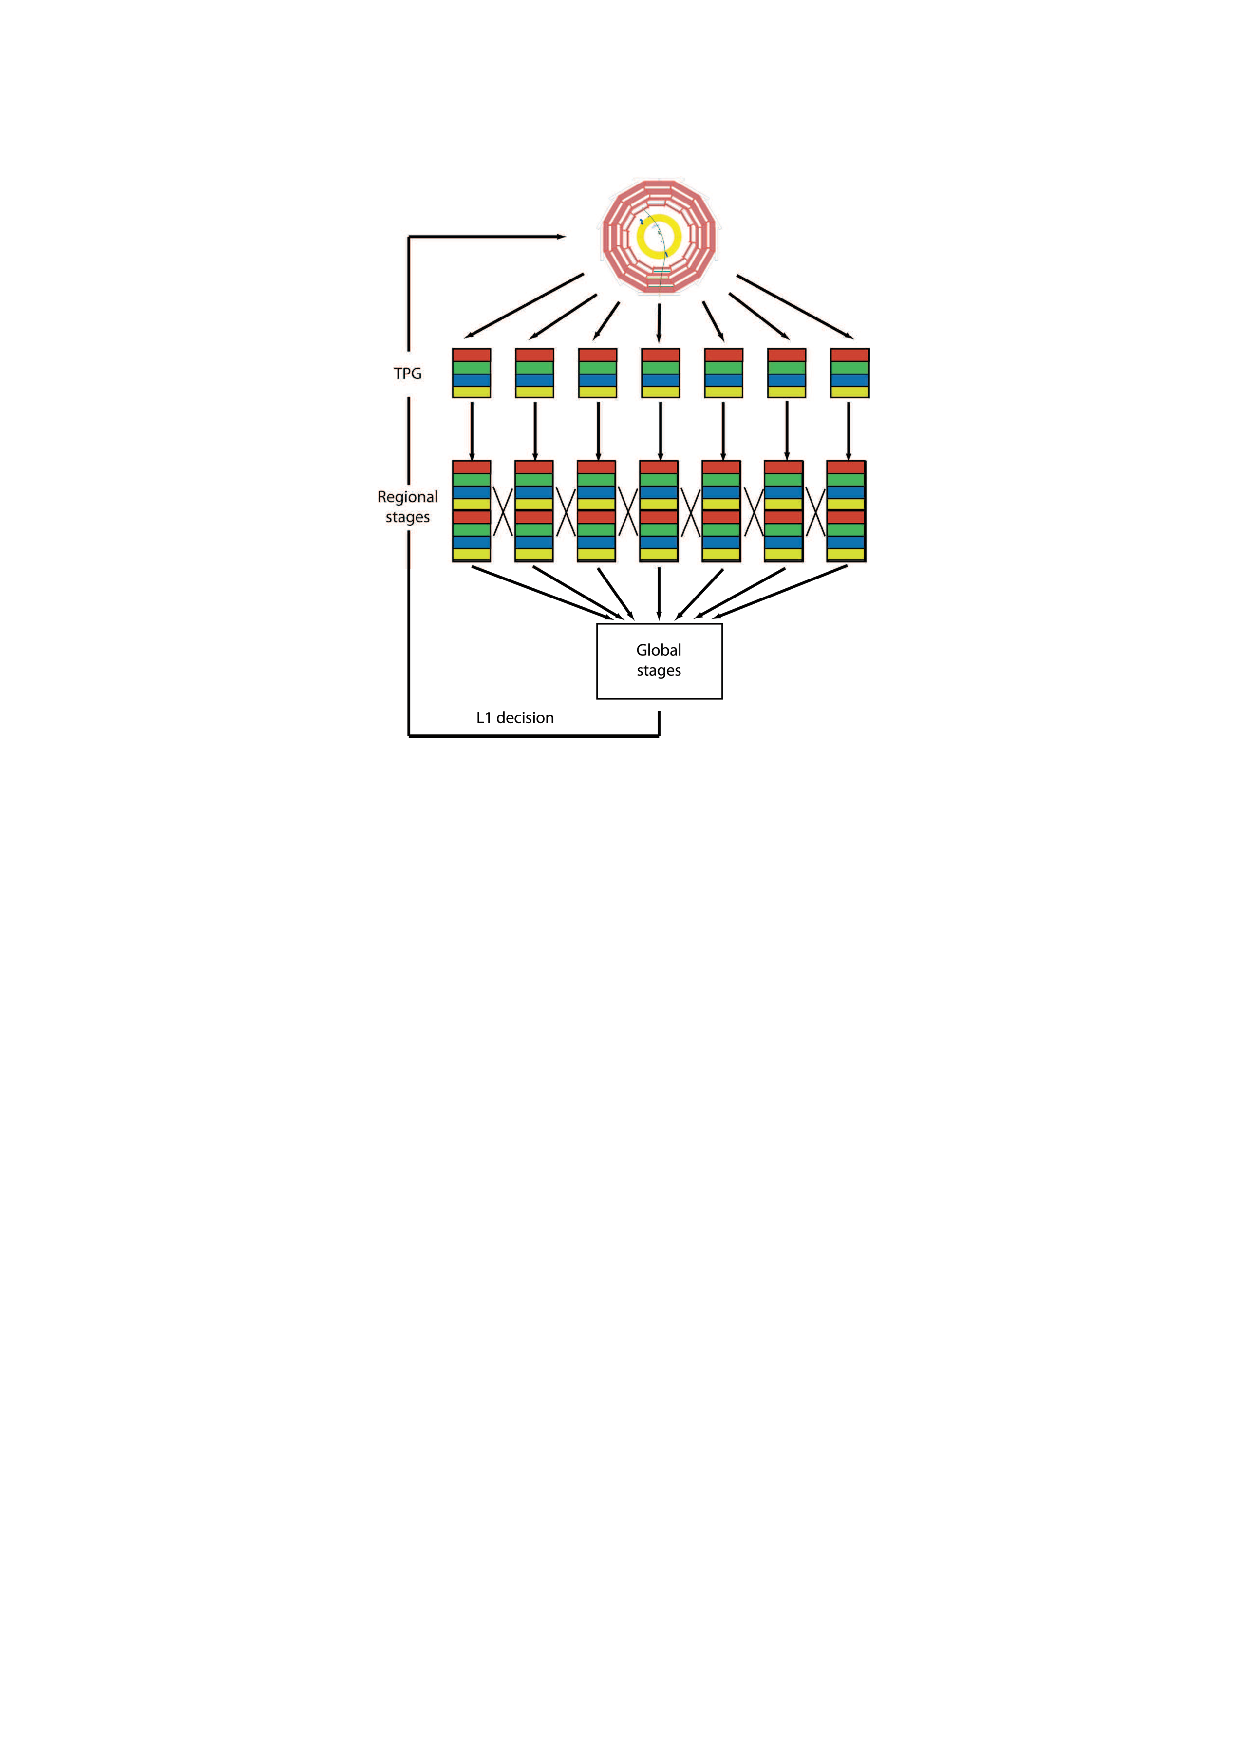
\includegraphics[width=0.4\textwidth]{figs/trigger/old_trigger}
  }~~
  \subfloat[Run~2 upgrade TMT trigger architecture.]{
    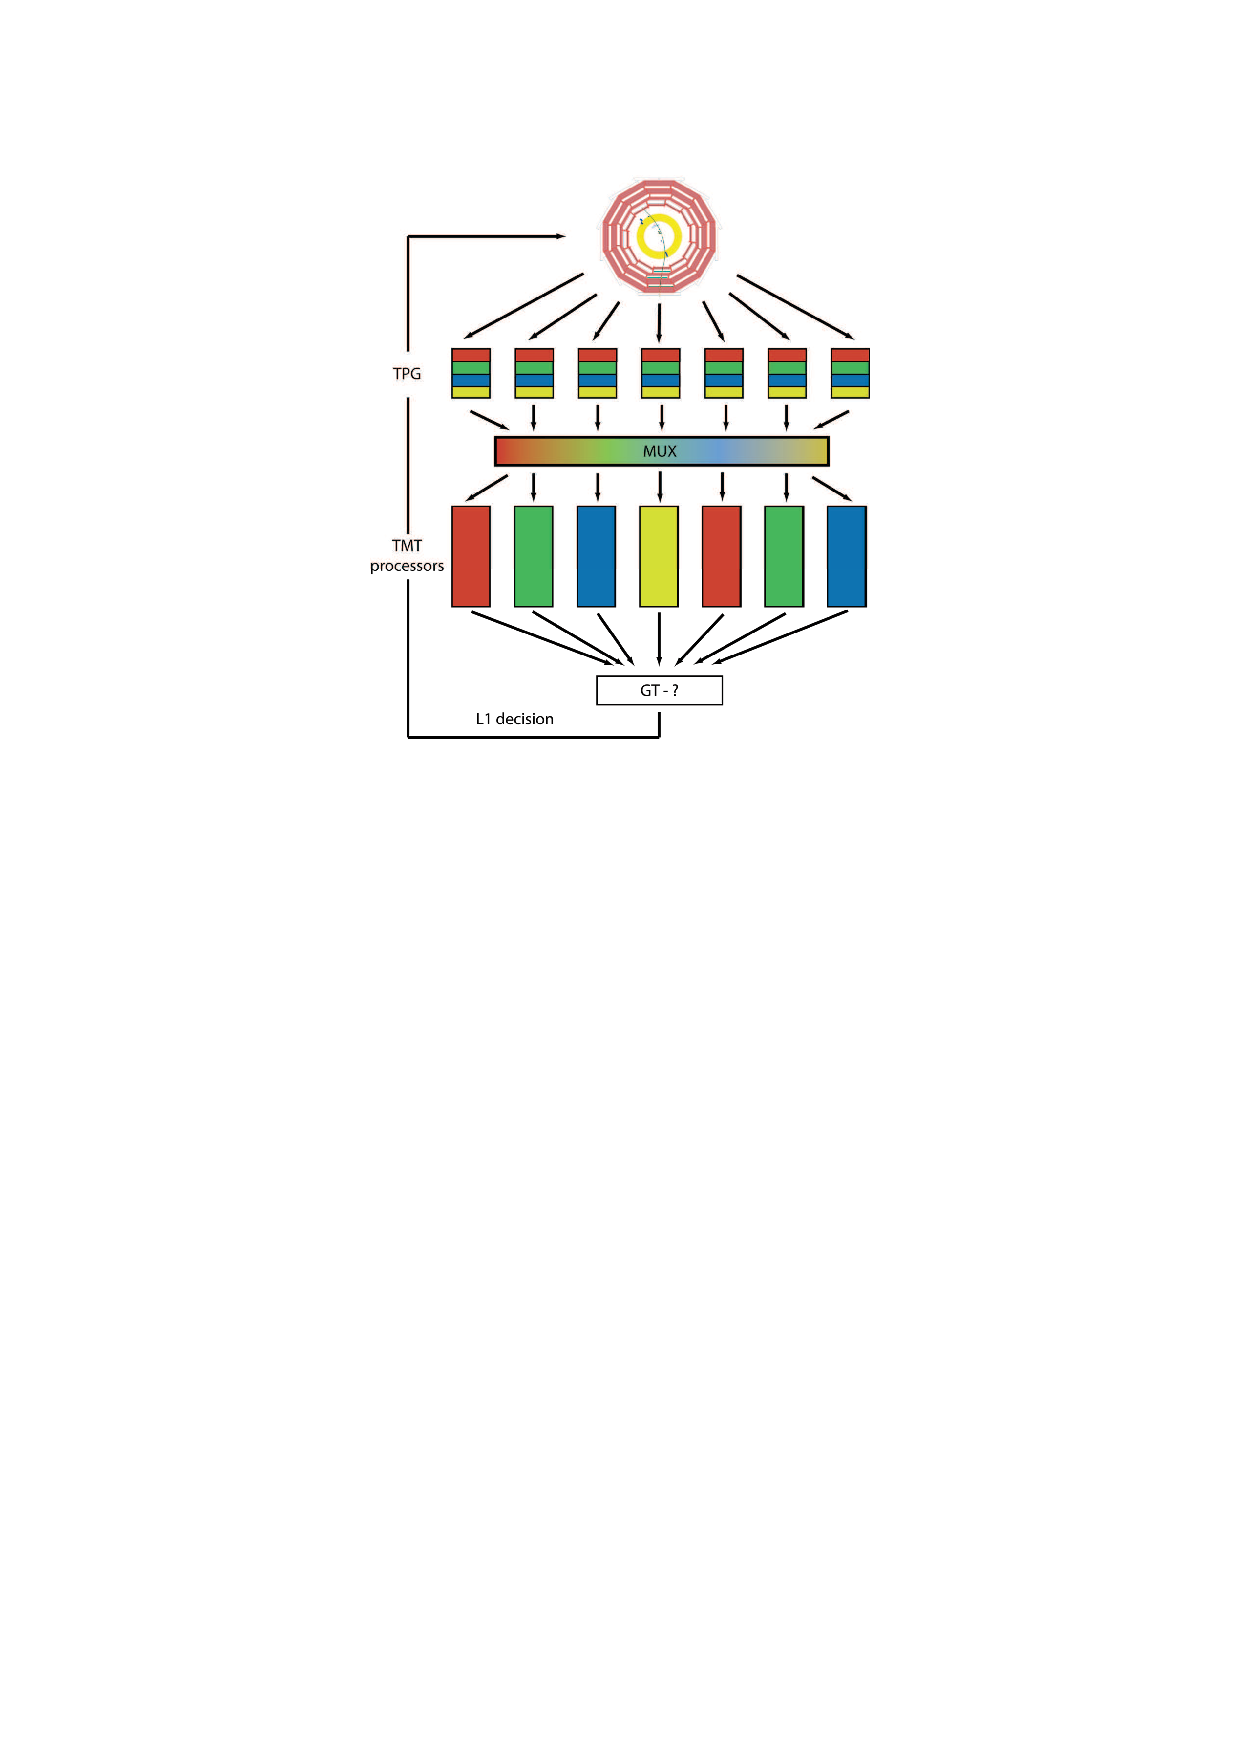
\includegraphics[width=0.4\textwidth]{figs/trigger/tmt}
  } \\
  \caption{A representation of the time multiplexed trigger (TMT)
  architecture (b) as opposed to the pre-upgrade trigger architecture
  (a). The entire information for one event is processed by one board
  rather than just parts of the detector for each board \cite{1748-0221-9-10-C10034}}
  \label{fig:tmt}
\end{figure}

The inputs to the Calorimeter Trigger from the various \ECAL and \HCAL
components are split into a $56\times 72$ grid of \TTs in $\eta$ and
$\phi$ within the barrel and endcap region ($|\eta|<3$), with each
tower covering the area of $5\times5$ \ECAL crystals.  As the
processing power of the \ac{GCT} was limited, for trigger calculations
the \TTs were grouped into $4\times4$ blocks, known as \emph{\ac{RCT}
regions} \cite{Khachatryan:2016bia}. These different regions are
visually represented in Fig.~\ref{fig:trigger_calorimeter}. Due to the
advantages brought by the upgrade, the new algorithms have access
to the full granularity information of all the \TTs. A representation
of the upgrade to the spatial resolution afforded by this change is
in Fig.~\ref{fig:sunnyJim}.

\begin{figure}
	\begin{center}
		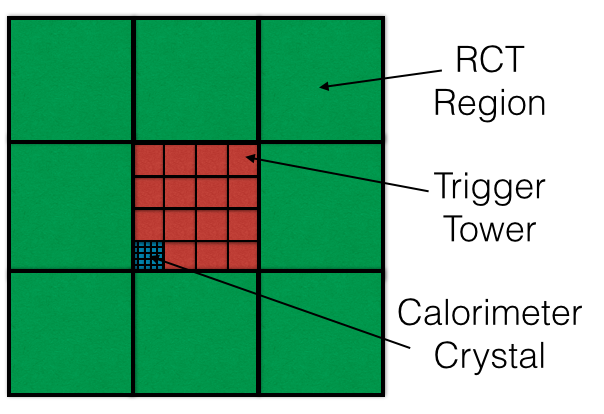
\includegraphics[width=0.5\linewidth]{figs/trigger/trigger_calorimeter}
	\end{center}
	\caption{The breakdown of the different calorimeter regions, the
  \ac{RCT} regions
  and trigger towers are both shown within the context of the \ECAL
  calorimeter crystals.}
	\label{fig:trigger_calorimeter}
\end{figure}

\begin{figure}
  \centering
  \subfloat[Run~1 calorimeter trigger resolution.]{
    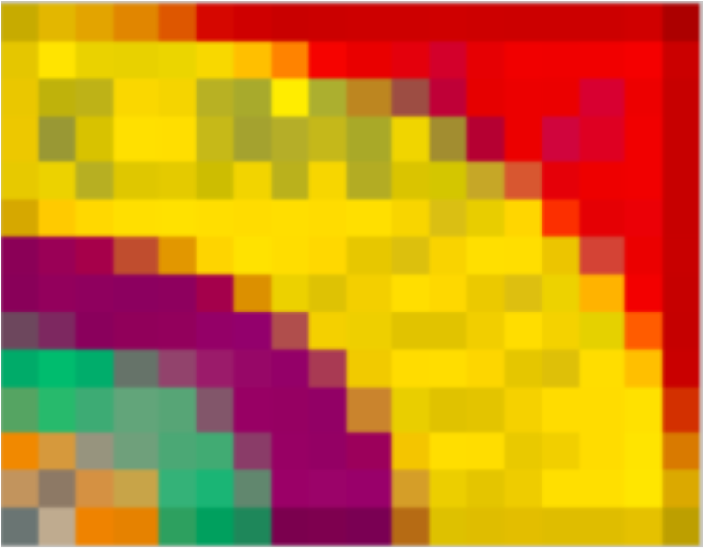
\includegraphics[width=0.35\textwidth]{figs/trigger/L1inputreslegacy}
  }~~
  \subfloat[Run~2 upgrade calorimeter trigger resolution.]{
    
\includegraphics[width=0.35\textwidth]{figs/trigger/L1inputresupgrade}
  } \\
  \caption{A representation of the spatial resolution of the trigger
  inputs to the calorimeter trigger for the Level-1 trigger before and
  after the upgrade.}
  \label{fig:sunnyJim}
\end{figure}

\section{The jet finder and energy sums}
\label{sec:jetFinder}

To make use of the potential brought by the Level-1 trigger upgrade,
new trigger algorithms are developed to improve the selection of
interesting physics processes. With a better view of the substructure
of energy deposits within the calorimeters, the identification of three
pronged tau jets and isolated electrons can be significantly improved,
for example \cite{egllr,taullr}. 

One area in which algorithm improvements can have a significant impact
is in the jet finding algorithm. As the Level-1 trigger must be of a
fixed latency, it cannot make use of an iterative algorithm such as
those used during offline jet-finding (described in
Sec.~\ref{sec:jets_reco}). In the algorithm used during Run~1, the jet
candidates are created from a $3\times3$ \ac{RCT} region sliding
window.  Candidates in which the central region has the maximum energy
are kept as jets \cite{Chatrchyan:2008aa}. These jets cover an area of
$\Delta\eta\times\Delta\phi = 1.04 \times 1.04$, which matches
reasonably well the area covered by circular jets with $R=0.5$, the
maximum radius for Run~1 offline jets.  To help mitigate the
reconstruction of jets originating from \PU, the central region of the
jet finder is also required to exceed a minimum energy, known as the
\emph{seed threshold}. Due to latency and processing power
constraints, there is no way in which contribution to the energy of
the jet from \PU can be subtracted dynamically. Along with the relatively
large jet size, this means the performance of the algorithm will be
severely reduced by the conditions present during Run~2. An upgrade
provides the extra processing power to carry out a dynamic \PUS,
correcting the energy of each jet from the influence of \PU. The
increased position resolution will also allow for a more accurate
determination of the direction of the jets.

Once a jet algorithm is chosen, the jets can be used to make Level-1
trigger decisions. This typically involves selecting events that are
observed to have jets, or sums of jets, with an energy above a certain
threshold. The selection made within the Level-1 trigger is
designed to pick out interesting physical processes, while removing
background events. The particular configuration of jets that lead
to an acceptance of an event is known as a \emph{trigger}. For
example, a single-jet trigger would require at least one jet above a
certain \pT threshold, or a quad-jet trigger would require at least
four jets above a certain threshold. The performance of the Level-1
trigger algorithms are therefore typically measured within this
context, as discussed in Sec.~\ref{sec:jet_algo_performance}.  When
designing these triggers, the total rate of acceptance of the Level-1
trigger cannot exceed a predefined value $\sim 100$~kHz. The sum of
the rates of all the trigger decisions must be kept below this number.
A trade off between all the potential triggers must be made, making it
of utmost importance to design triggers with manageable rates.

\subsection{The upgraded jet algorithm}
\label{sec:stage2_jetalgo}

The jet algorithm for the Run~2 CMS trigger upgrade operates on
the sum of the \ECAL and \HCAL energy deposits in the \TTs. The studies
in this Chapter consider the \TTs within $|\eta|<3$.
% , with the potential
% to extend the algorithm up to $|\eta|<5$. 

Starting with a similar idea as in Run~1, the upgrade makes use of a
sliding window algorithm. In the upgrade, however, the window
considered is a $9\times9$ square of \TTs, covering
$\Delta\eta\times\Delta\phi = 0.78 \times 0.78$. This odd number of
trigger towers results in an easily defined central tower as well as
matching the area covered by the $R=0.4$ offline jets that are used in
Run~2. Within a window the central tower is considered as the
direction of a candidate jet. The candidate is vetoed if any of the
other \TTs in the square have an energy deposit of either greater than
or, in some cases, equal to it. The veto condition is
antisymmetric along the diagonal of the square to prevent \TTs with the
same energy from vetoing one another. A representation of the window
considered can be seen in Fig.~\ref{fig:stage2_jetalgo}.  Any \TTs that
pass this criterion are considered as jet centres, where the jet energy
is equal to the sum of all the towers within the $9\times9$ square.
% Taking the highest energy
% TT as the centre of the jet axis is motivated by the fact that jets
% are boosted objects with most of their energy in the middle
% \cite{JetProfile_pileup}.

The veto conditions applied on the central \TT ensure that no two
overlapping jets are reconstructed, avoiding the duplication of energy
deposits. However, the algorithm can introduce inefficiencies in very
specific jet topologies. In these cases a high energy \TT vetoes a
medium energy \TT which then vetoes a lower energy \TT. 
The medium energy \TT is included in the jet constructed by the high energy
\TT, however the lower energy \TT is lost. This is not usually a
problem when making decisions with the Level-1 trigger, as the high
energy \TT will usually ensure that the event is triggered, despite
energy being lost.

\begin{figure}
	\begin{center}
		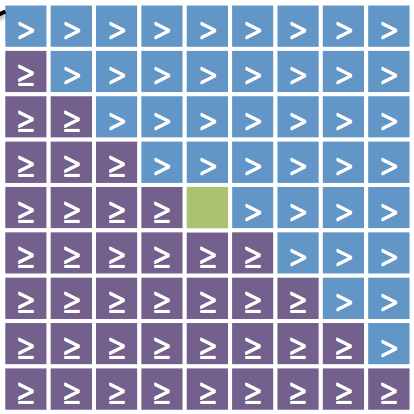
\includegraphics[width=0.3\linewidth]{figs/trigger/stage2_jetalgo}
  \end{center} \caption{The consideration of a Trigger Tower candidate
  for the upgrade Level-1 Trigger jet algorithm. The candidate (green)
  is vetoed if the energy of the other towers meets the condition
  shown in the blue and purple towers.}
	\label{fig:stage2_jetalgo}
\end{figure}

\subsection{A comparison with the offline jet algorithm}

In order to test the performance of the upgrade algorithm it is compared to
jet finding with anti-$k_T$ clustering, the most popular algorithm
for offline jet reconstruction. As the Level-1 algorithm has less
sophisticated inputs than the \PF candidates used offline, the
anti-$k_T$ algorithm is used to find jets with the \TTs as input. The test was
carried out on a $t\bar{t}$ \MC simulation, which contains a high
multiplicity of jets that are produced in top-quark decays. The performance of
the algorithm compared to anti-$k_T$ jet clustering with $R=0.4$ can
be seen in Fig.~\ref{fig:ak4_comp}. For the jet with the highest \pT,
the leading jet, the distributions of \pT and $\eta$ are very similar
for both the jet finding algorithms. For the fourth-leading jet more
differences emerge at low \pT and the edges of the $\eta$
distribution. This is probably due to the ability of the anti-$k_T$
algorithm to adaptively fit smaller radius jets and those at the edge
of the detector acceptance.

\begin{figure}
	\begin{center}
		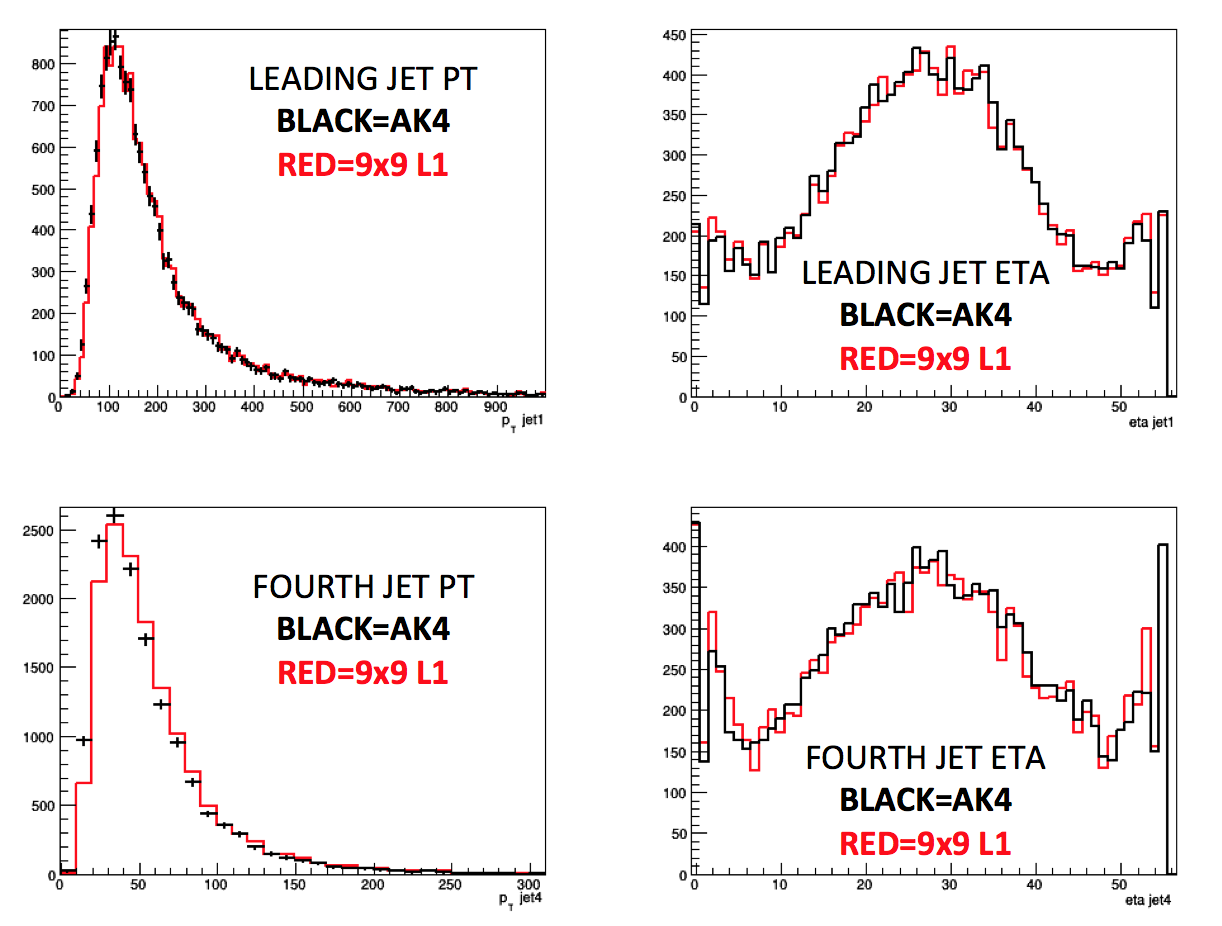
\includegraphics[width=1.0\linewidth]{figs/trigger/jet_l1s2_compak4}
	\end{center}
  \caption{A comparison between the upgrade Level-1 trigger ($9\times9$L1) jet
  algorithm and the anti-$k_T$ offline algorithm with R=0.4 
  (AK4), taking
  the \TTs as input.  These plots are produced from a
  $t\bar{t}$ simulation with $13$~TeV proton collisions and \PU $\sim40$.
  The units for the pseudorapidity are in trigger tower units, which
  range from 0 at $\eta =-3$ to 56 at $\eta=3$.}
	\label{fig:ak4_comp}
\end{figure}

\subsection{Energy sums}

Along with finding jets in an event, the Level-1 trigger is required
to calculate energy sums, analogous to those discussed in
Sec.~\ref{sec:met_reco}.  These energy sums can take either the jets
or \TTs as input. They include:
\begin{itemize}
\item{total $E_T$, the scalar sum of the transverse energy in all the
\TTs}
\item{\met, the negative vector sum of the transverse energy in all the
\TTs}
\item{\HT, the scalar sum of all the Level-1 jets}
\item{\MHT, the negative vector sum of all the Level-1 jets}
\end{itemize}

\section{Pileup subtraction}
\label{sec:pus}

\subsection{Characterising pileup}
 
On average, the decays from \PU are expected to be isotropically
distributed around the detector. However, there will be significant
event-by-event differences due to Poisson fluctuations in the number
of \PU collisions. While the number of simultaneous interactions is
such that these fluctuations are significant, it is advantageous to
correct for the \PU on a per-event basis. To be able to remove the
effects of \PU in the Level-1 trigger there needs to be a way to remove
the objects that originate from \PU. Additionally, an
estimate of the average energy deposited in each event should be used
to correct the $E_T$ of the remaining objects. These procedures are
known collectively as \emph{\acf{PUS}}.

It is observed that the density of decays from \PU 
depend on their position in $\eta$ \cite{Cacciari2011}. This is
most likely caused by the differing response of the detector along its
length. The fact that the trigger only has access to
coarse calorimeter information and no tracks means these detector
effects are likely to be enhanced. It is therefore desirable for \PUS
algorithms to measure the \PU energy density near to the objects that
are corrected. This \emph{local} \PUS then requires a trade off
between the proximity to the object and the effects of the
larger statistical fluctuations from sampling a smaller area. 

A \emph{global} subtraction can be used to determine the average
energy density across the whole detector. This method is much less
susceptible to fluctuations and contamination from particles from the
hard-interaction, but does not take account of local fluctuations or
detector effects.

The ideal form of \PUS will remove the dependence of the Level-1
trigger rate and efficiency on the number of simultaneous interactions
in an event. It should do this in a way that improves the resolution
of object energy measurements, increasing the acceptance
of interesting physics events while allowing for the rejection of soft
QCD multijet processes. It is also important to take account of the
Level-1 trigger architecture when designing the algorithm to ensure
that it can be performed with a fixed latency. Different forms of \PUS
in the Level-1 trigger are outlined in this section and their
performance subject to these criteria is examined in
Sec.~\ref{sec:jet_algo_performance}. 

As well as mitigating \PU from simultaneous collisions, the effects of
\ac{OOTPU} must be removed. This is predominantly achieved during the
generation of the \TT inputs for the calorimeter trigger. When reading
out the energy deposited in the \ECAL and \HCAL the average extra
energy deemed to have come from a previous bunch crossing is
subtracted and a correction factor is applied. This mitigation
performs well enough to make the effects of \ac{OOTPU} subdominant
with respect to in-time \PU.

\subsection{Global pileup subtraction}

A prominent method of \PUS is $\rho$-area correction
\cite{Cacciari:2007fd,Cacciari:2008gn}. It works by finding the
average energy per unit area in the calorimeter due to PU, $\rho$, and
subtracting it from each reconstructed jet. A favoured estimator for this
quantity is:
\begin{equation}
\rho\equiv median(\frac{p_{Tj}}{A_j}),
\end{equation}
where $p_{Tj}$ is the transverse momentum of a jet $j$, $A_j$ is its
area and the median is taken over all reconstructed jets in an event.
In the plots in this chapter, this form of \PUS is known as \emph{global}. It
acts to remove half the jets in an event, the low energy half, and
correct down the energy of the remaining half. This works
particularly well in high \PU cases as $\rho$ is insensitive to
fluctuations in the energy of interesting physics events. 
% It is
% possible to take account of $\eta$ dependence through a new variable
% \emph{local $\rho$}, where the different values are calculated in
% different $\eta$ ranges of the detector. This method loses robustness
% as the number of jets that are sampled is lowered for each $\rho$
% calculation.

The mean value of \rho, as a function of the number of interactions,
is shown in Fig.~\ref{fig:rho}. This is taken from a minimum bias \MC
simulation in which there is no visible hard interaction but only
overlaid \PU collisions. There is a good correlation between the
number of simultaneous collisions and \rho, indicating that it is
indeed a reasonable measure of the \PU in the event. The correlation
also passes through the origin, indicating that \ac{OOTPU} is not a
problem with a 50~ns bunch spacing.

\begin{figure}
	\begin{center}
		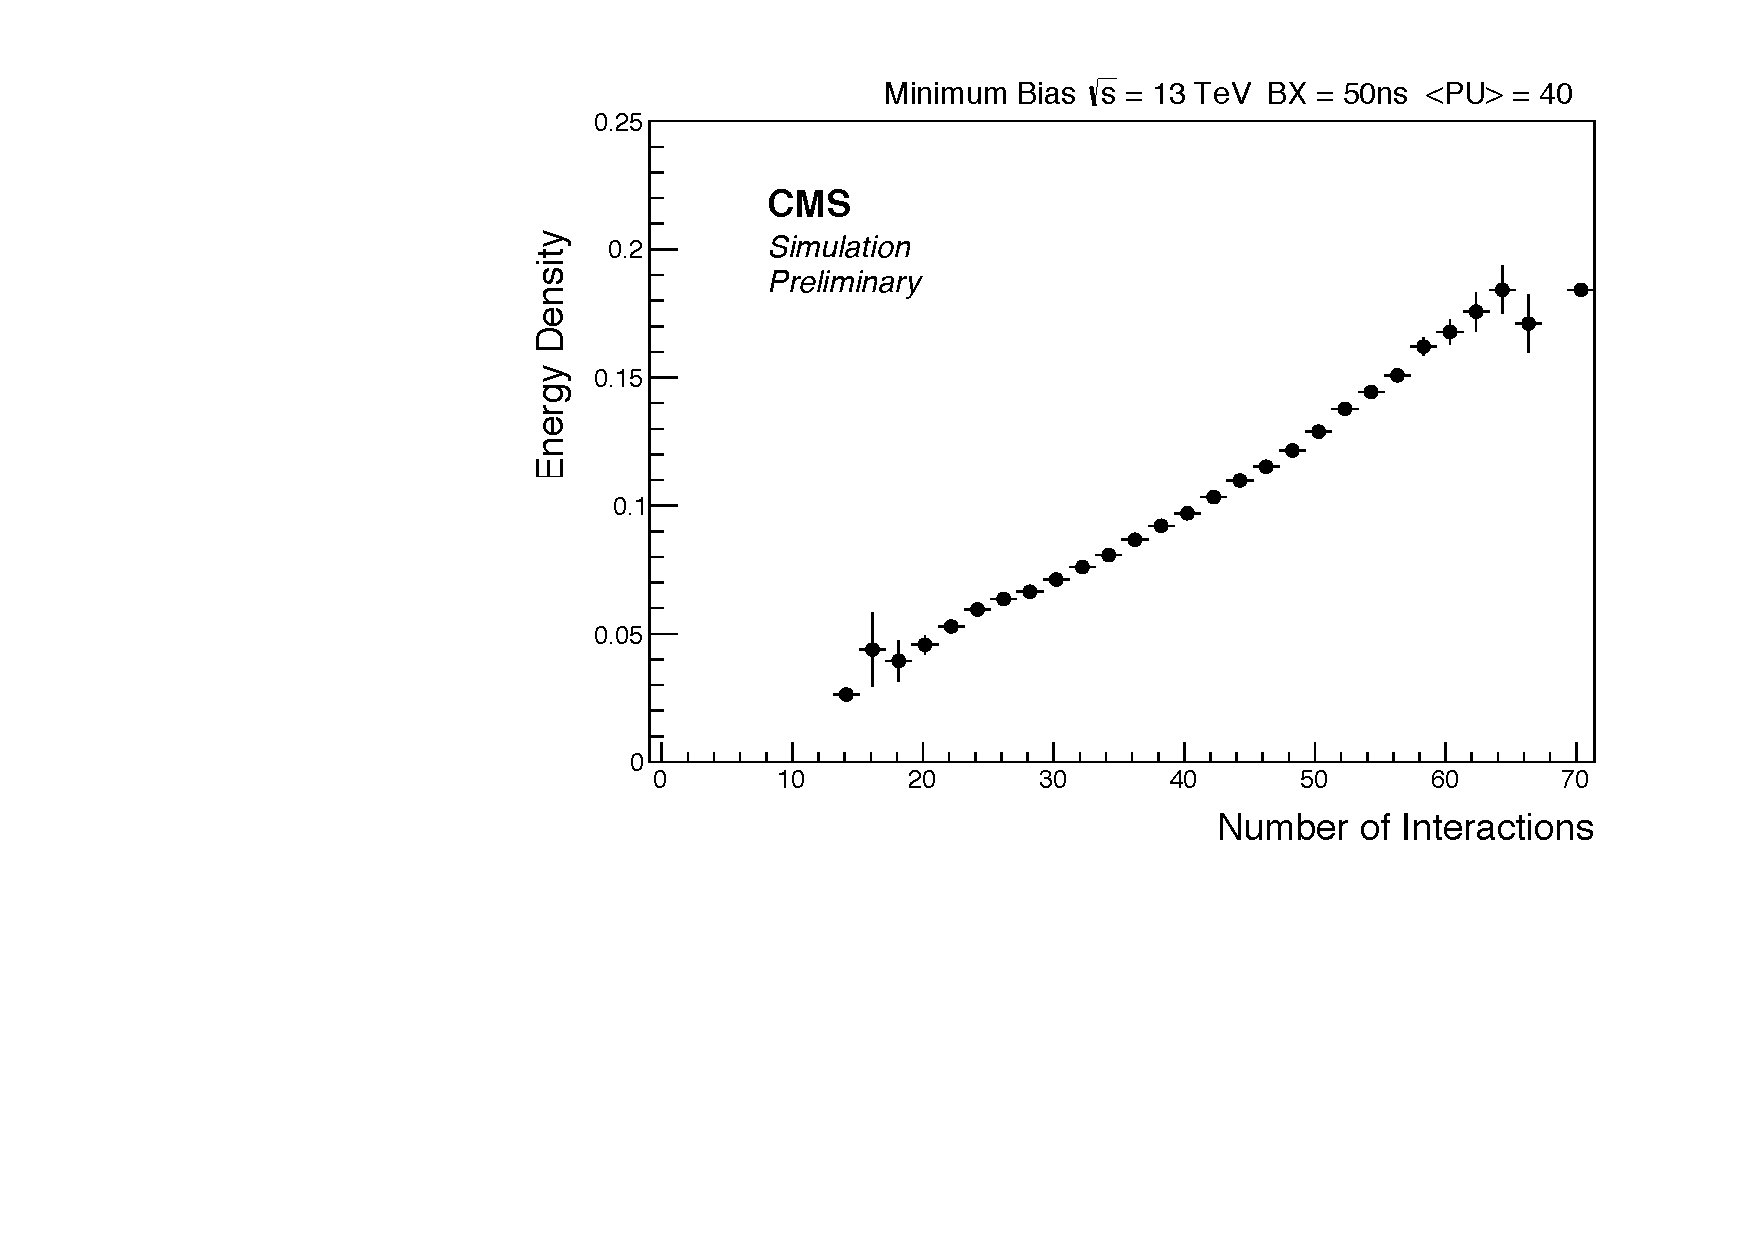
\includegraphics[width=0.8\linewidth]{figs/trigger/median}
  \caption{The median energy density, \rho, of Level-1 jets in the \CMS
  calorimeters as a function of the number of simultaneous collisions.
  This is taken from minimum bias \MC simulation at 13~\tev with a
  50~ns bunch crossing time}
	\label{fig:rho}
	\end{center}
\end{figure}

Subtraction with the $\rho$-area method has a latency penalty when
implemented in hardware as the jets must be found before \rho can be
calculated and subtracted from their energies. Depending on the final
firmware designs this can present a problem and makes global \rho
subtraction harder to perform in hardware. Despite this fact, as
global \rho is a popular and well understood form of offline \PUS it
acts as a good benchmark against which to test other algorithms.

\subsection{Donut Subtraction}

As jets from the hard scatter are typically boosted objects, most of
their energy is deposited very close to the central \TT of the jet
algorithm \cite{JetProfile_pileup}. A typical energy profile of a jet
is shown in Fig.~\ref{fig:jetprofile}. In the case of isolated jets,
the ring five \TTs from the centre of the jet can be assumed to contain
only contamination from \PU.  The \emph{donut subtraction} algorithm
therefore takes the
energy per unit area in the ring of \TTs surrounding the jet (shown in
Fig.~\ref{fig:donutstrips}) and scales
it up by the area of the jet. The resulting energy is then subtracted
from the jet to correct any \PU contamination. This kind of \PUS has
been applied in the analysis of heavy ion collisions at the \LHC
\cite{Cacciari:2010te}.

\begin{figure}
	\begin{center}
		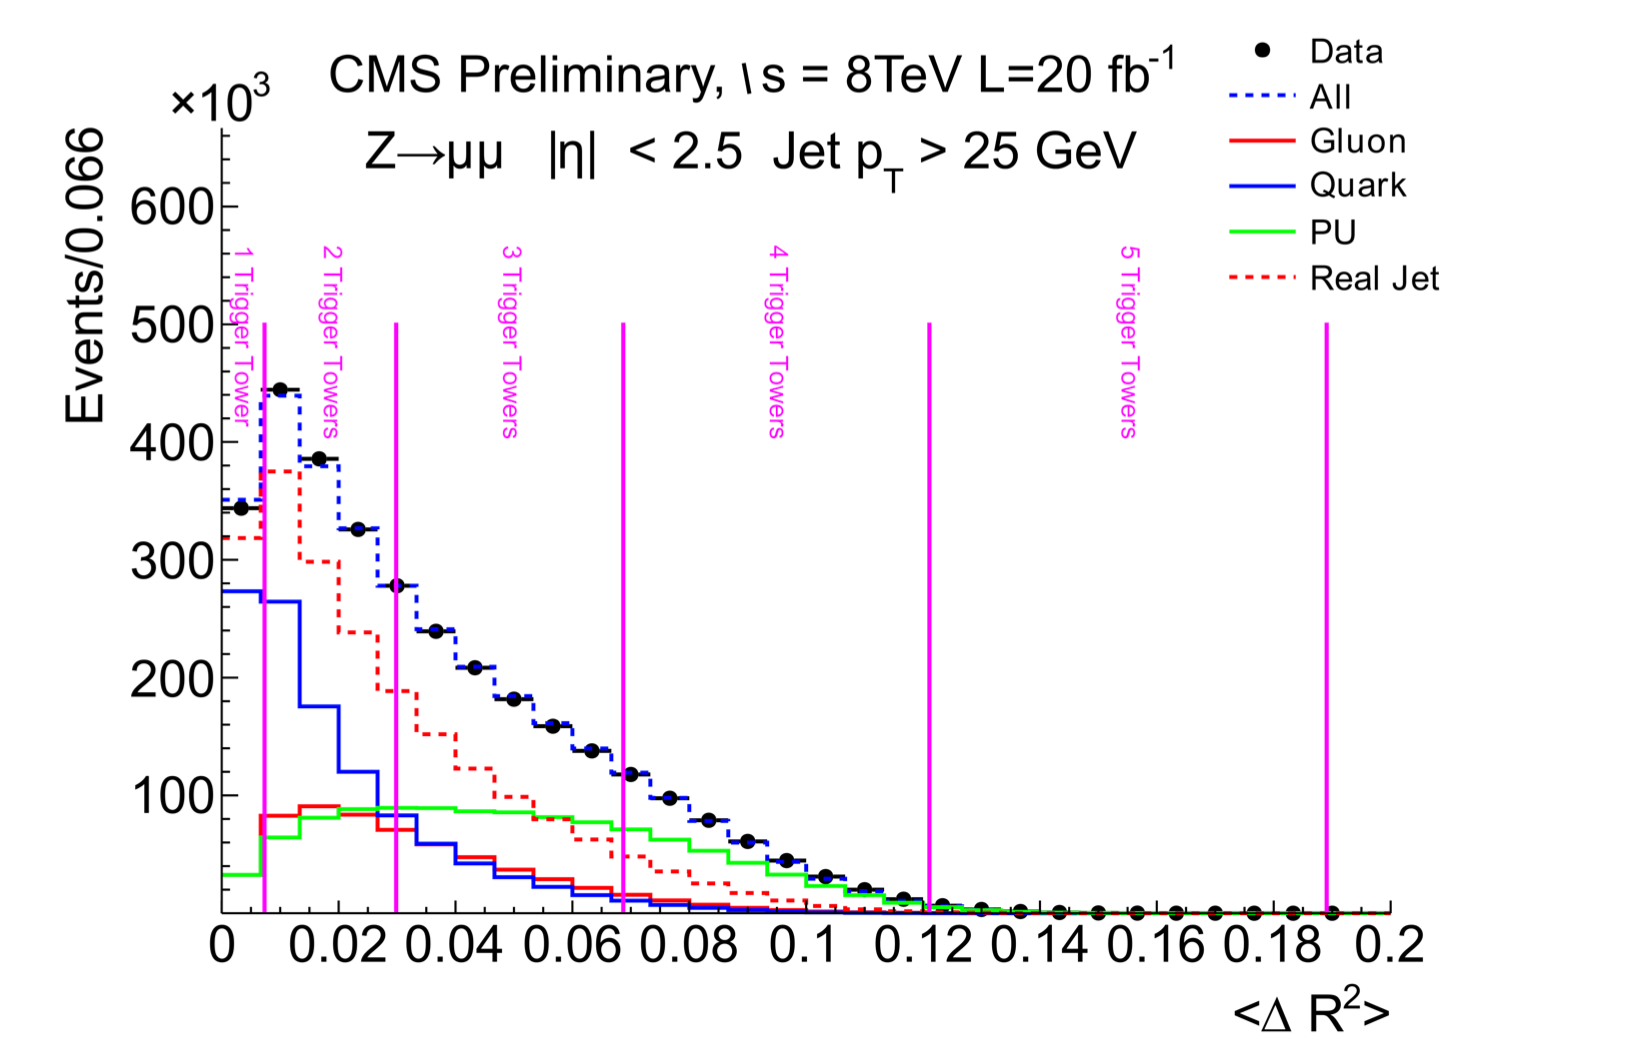
\includegraphics[width=0.8\linewidth]{figs/trigger/jetProfile}
  \caption{ Jet energy profile as a function of the squared distance from the
  centre of the jet, $\Delta R^2$. The number of trigger towers that the
  distances corresponds to are shown in pink. Calculated for jets from
  a simulation of Z to $\mu\mu$ events \cite{JetProfile_pileup}}
	\label{fig:jetprofile}
	\end{center}
\end{figure}

This approach only works for correcting isolated jets, if one jet from
the hard-scatter is
in the vicinity of another, the energy in the donut can be increased to
above that of \PU. To mitigate this, only the median two $4\times1$
\TT strips of the four that make up the donut are used to calculate
the \PU energy density. This reduces the chance that energy from
another jet will be counted as \PU and also removes strips that have
very little energy in them from a downward fluctuation in \PU
contamination. An example of the two strips that could be selected can
be seen in purple in Fig.~\ref{fig:medianstrips}.

\begin{figure}
  \centering
  \subfloat[Strips considered for donut subtraction.]{
    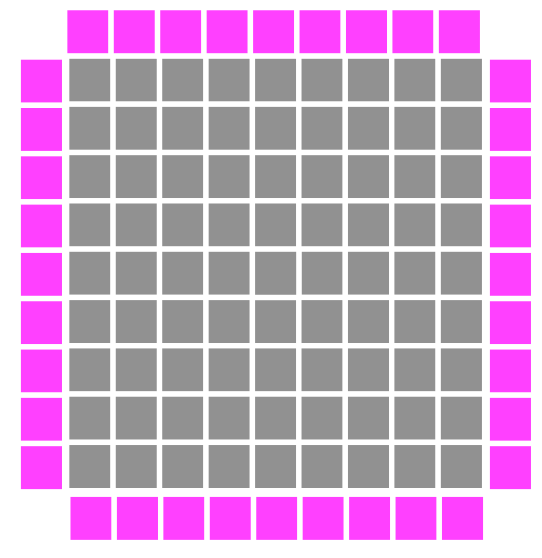
\includegraphics[width=0.3\textwidth]{figs/trigger/donut}
    \label{fig:donutstrips}
  }~ 
  \subfloat[Example of median energy strips.]{
    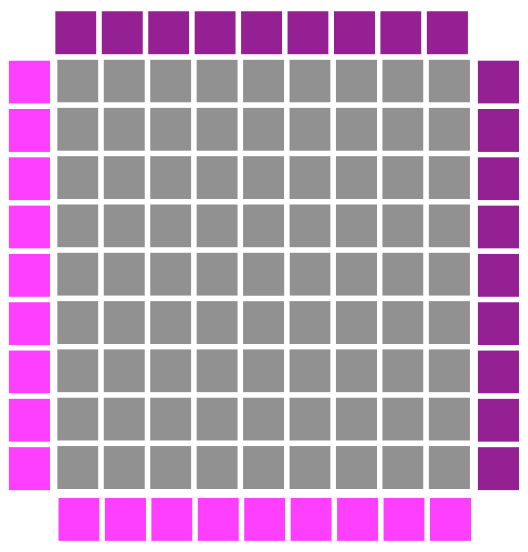
\includegraphics[width=0.3\textwidth]{figs/trigger/donut2}
    \label{fig:medianstrips}
  }~
  \subfloat[Strips considered for chunky donut subtraction.]{
    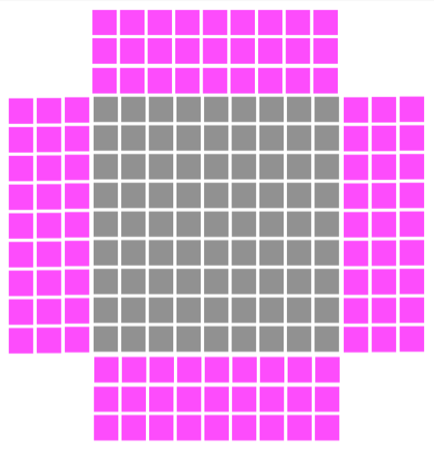
\includegraphics[width=0.3\textwidth]{figs/trigger/chunkyDonut}
    \label{fig:chunkystrips}
  }\\
  \caption{Various configurations of \TT strips around the Level-1 jet
  algorithm window used for donut subtraction}
  \label{fig:alldonutstrips}
\end{figure}

One of the main issues with the donut subtraction algorithm is this
sensitivity to fluctuations. It is mitigated by taking the median energy two strips
but can be further reduced by increasing the area covered by the
strips. The rings of \TTs can be extended to be three towers wide,
known as a \emph{chunky} donut and illustrated in
Fig.~\ref{fig:chunkystrips}. This is particularly effective in
reducing the fluctuations in the positions of \PU particles with
respect to the jet in consideration.

To confirm that the energy in the median two strips of the  chunky
donut is a good measure of the \PU in the event, it is plotted against
the number of interactions for a minimum bias \MC sample in
Fig.~\ref{fig:donut_nint}. There is a good correlation that appears to
pass through the origin, implying it is indeed a good measure of \PU. 
% note that the fact that it passes through the origin for ttbar
% indicates that the median strips reduce hard scatter contamination

\begin{figure}
	\begin{center}
		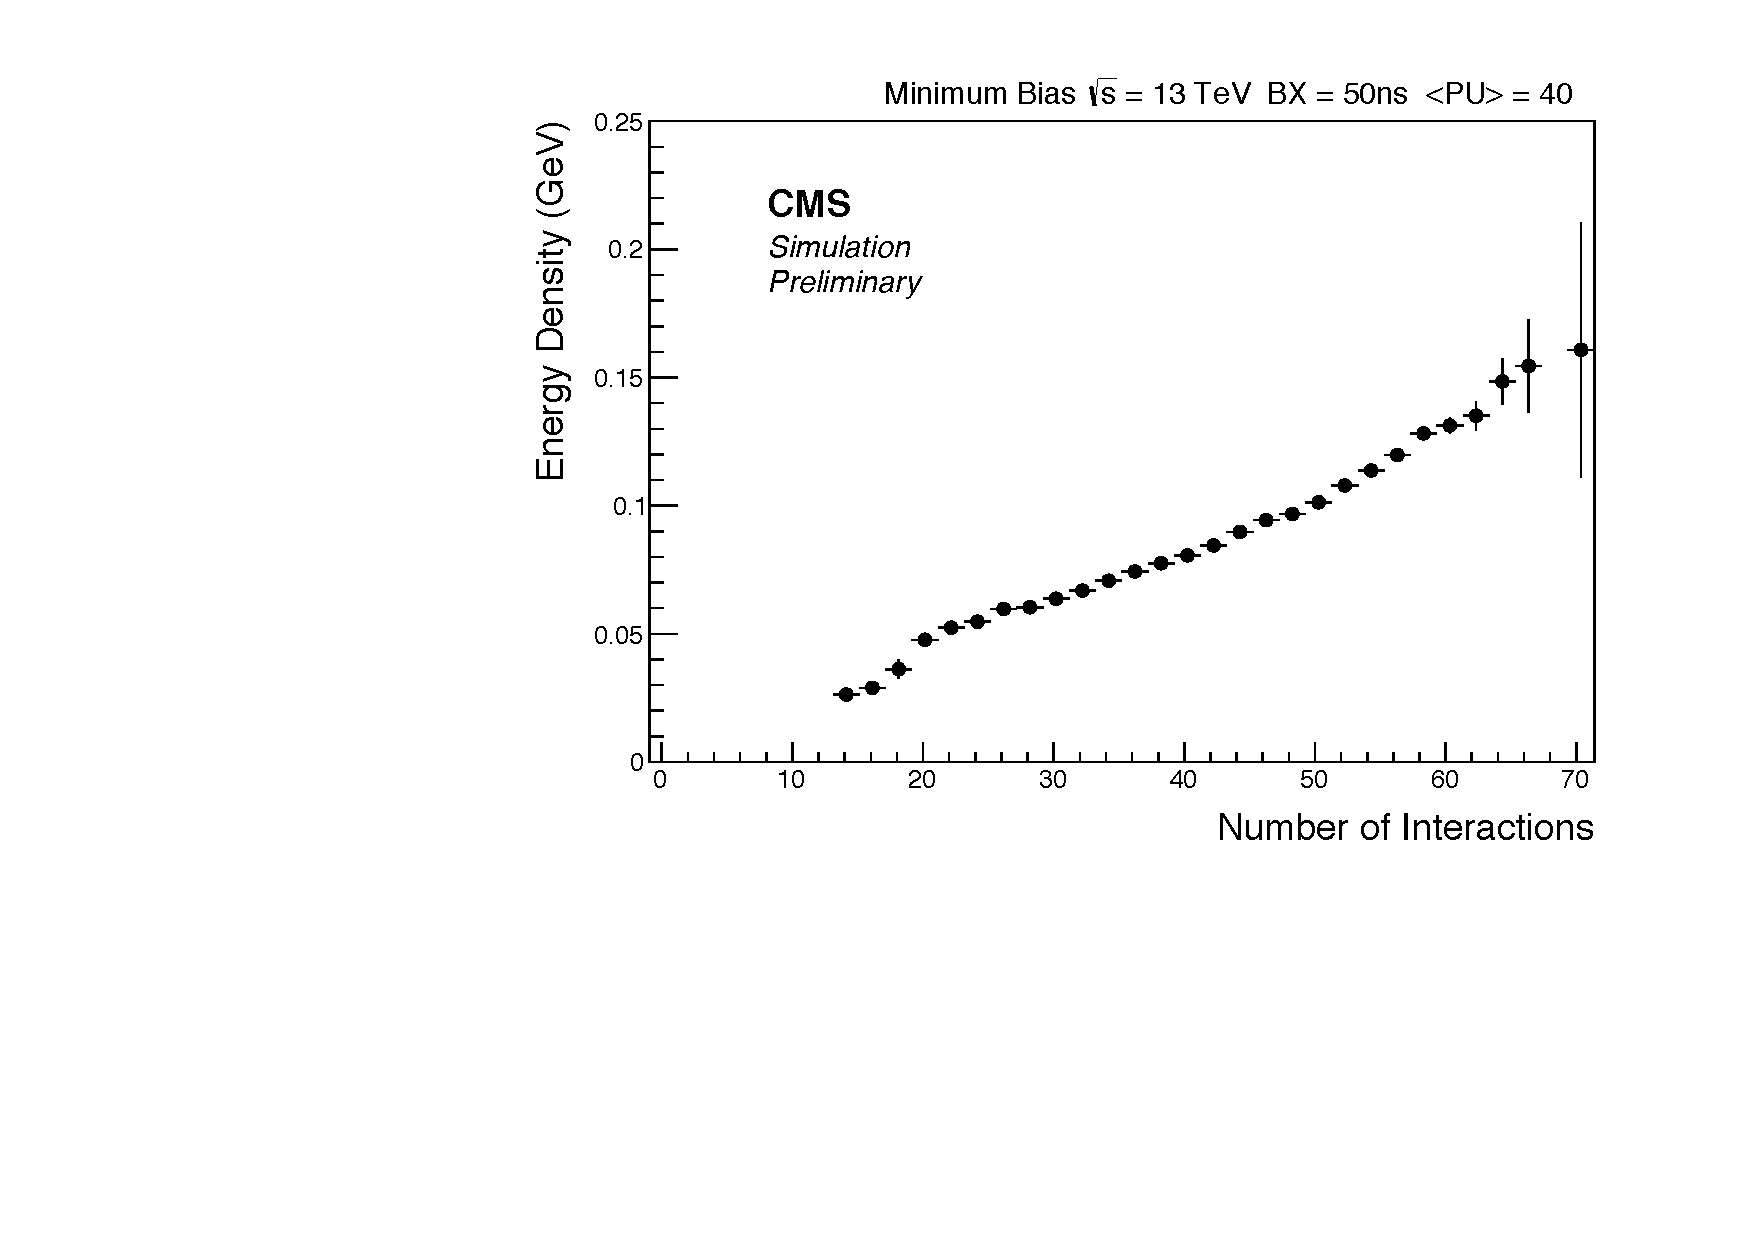
\includegraphics[width=0.8\linewidth]{figs/trigger/threestrips}
  \caption{The energy density in the median two $3\times 1$ \TT strips
  of a chunky donut around Level-1 jets in the \CMS calorimeters as a
  function of the number of simultaneous collisions. This is taken
  from minimum bias \MC simulation at 13~\tev with a 50~ns bunch
  crossing time}
	\label{fig:donut_nint}
	\end{center}
\end{figure}

In the implementation of the Level-1 jet finding algorithm in the
upgrade hardware, the \TTs that make up the donut are already
available in memory. This means donut subtraction has a very low
latency penalty. This presents a significant advantage over a global
\PUS. 

\subsection{Jet seed threshold and zero suppression}

Donut subtraction helps to remove the effects of \PU on the
reconstructed high energy jets, but is less successful at removing the
soft jets that are purely from \PU interactions. A simple way of
reducing the number of soft jets is by introducing an energy threshold
on the \TT that can form a jet. The \TT that is considered for a jet
candidate in the algorithm outlined in
Section~\ref{sec:stage2_jetalgo} is required to be above a certain
energy, known as the seed threshold. This is very easy to implement in
hardware, and has the potential to save latency as it reduces the
number of jets that need to be made. A disadvantage is that it can
kill soft jets that originate from a primary vertex. It also does not
account for any $\eta$ dependence. For the studies in
Sec.~\ref{sec:jet_algo_performance} a seed of $2.5$~GeV was
chosen as a benchmark that appeared to kill PU jets without removing
jets above 10~GeV from a zero PU $t\bar{t}$ \MC simulation. This is
demonstrated in Fig.~\ref{fig:noPUSeedTTbar}. As the Level-1 hardware
measures energy in units corresponding to 0.5~\gev (\emph{L1-units}),
this is denoted as \emph{Seed 5}. 

\begin{figure}
	\begin{center}
		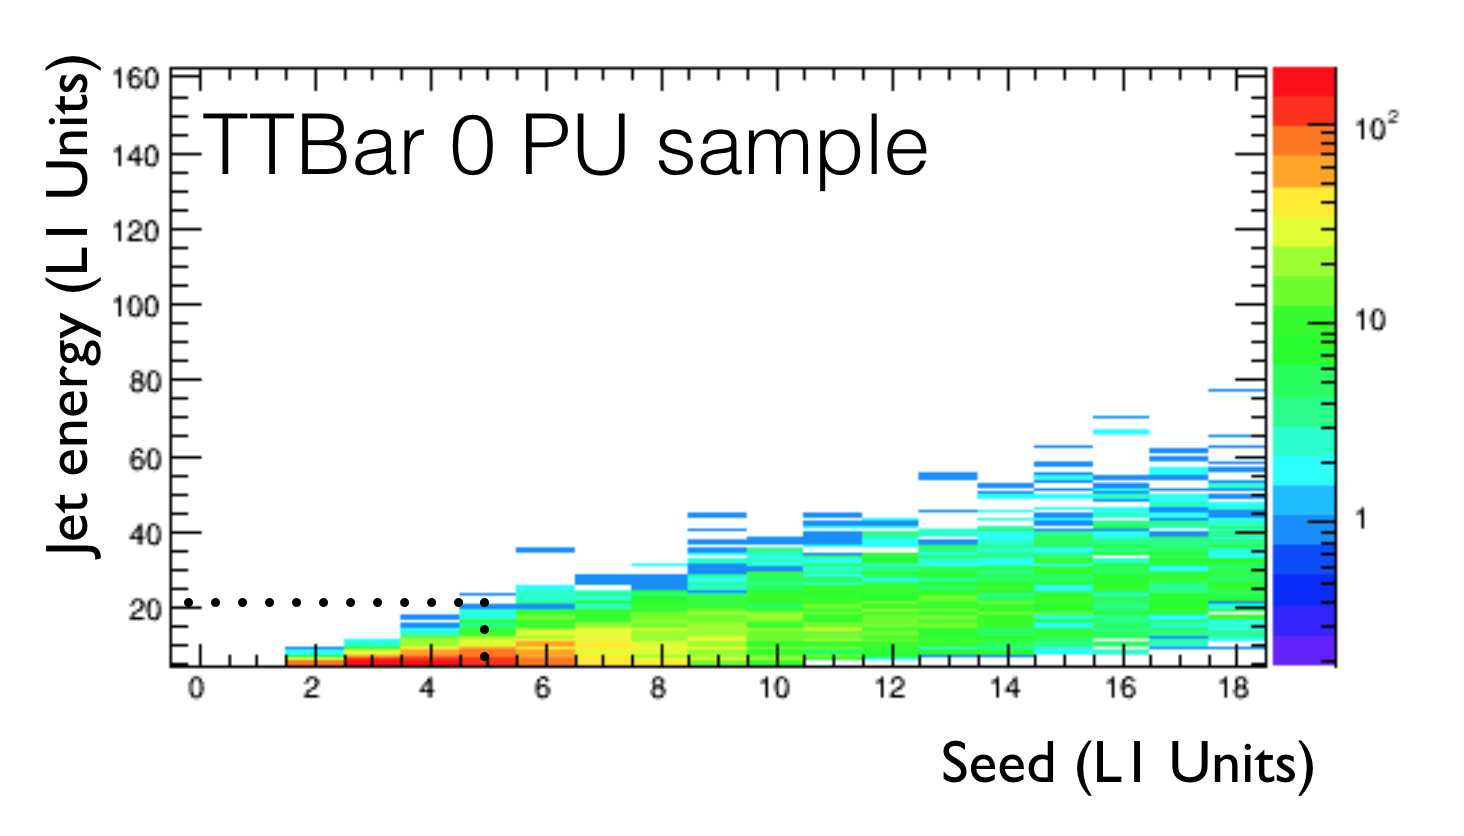
\includegraphics[width=0.8\linewidth]{figs/trigger/noPUSeedTTbar}
  \caption{The Level-1 jet energy vs seed threshold for a simulated
  sample of top quark pair production events with no overlaid \PU. The
  units of energy are \emph{L1-units}, which correspond to 0.5~\gev
  each. A seed threshold of 2.5~\gev only removes up to 10~\gev jets
  from the hard scatter.}
	\label{fig:noPUSeedTTbar}
	\end{center}
\end{figure}

To remove the effects of noise on the Level-1 trigger inputs, a
\emph{zero-suppression} is performed that requires \TTs to have an
energy above 0.5~\gev before they are considered to have any energy at
all. As \PU is expected to result in much smaller energy deposits than
interesting physics processes, the effect of increasing the energy
that is suppressed to zero when building the jets also acts as a form
of \PUS. This form of \PUS is considered in
Sec.~\ref{sec:jet_algo_performance} and is named Tower Suppression
(TSup). Despite being very easy to implement in hardware this
algorithm does not adapt well to different \PU conditions and can
reduce the energy resolution of the jets.

\section{Level-1 jet energy calibration}
\label{sec:l1jec}

To obtain Level-1 jets that correspond as closely as possible to the
true physics objects that they represent, their energy must be
corrected. The
varying response of the \HCAL and \ECAL as a function of jet \pT and
\eta necessitates a calibration that depends on these variables.  The
need for calibration in the Level-1 trigger is exacerbated by the
coarse level of information available compared to that in offline
reconstruction.

The calibration is performed using QCD dijet \MC simulation with an
average \PU of 40. Samples were generated with a range of generator
scales from 10 to 600~\gev. These energies characterise the \pT of the
leading jet and ensure a wide range of jet energies are available.
From this sample, \emph{generator jets} are clustered from
the truth-level particles, the final result of the procedure
described in Sec.~\ref{sec:mc_reco}. Clustering is performed with the
anti-$k_T$ algorithm with $R=0.4$, after removing any muon and
neutrino particles. This ensures that the Level-1 jets are just
calibrated based on the particles that are deposited in the
calorimeters. The Level-1 jet algorithm is performed on the simulated
Level-1
trigger calorimeter inputs. Each Level-1 jet is matched to the
generator jet that is closest in $\Delta
R=\sqrt{(\Delta\eta)^2+(\Delta\phi)^2}$ to the central \TT of the jet.
If a generator level jet cannot be found within $\Delta R<0.3$, the
Level-1 jet in question is ignored. The \pT of the Level-1 jet
(L1~\pT) after \PUS is compared to the \pT of the generator jet
(GEN~\pT) and the response is defined as the ratio of these two
quantities, L1~$\pT/$GEN~\pT.
% from Kristian via Adinda about what the PT hat is:
% The is the Pt scale of the "internal quark line" in the Feynman
% diagram for QCD multi-jet production.
% It sets a typical scale of the highest Pt jet, but in most events
% there will be softer jets from parton showers in addition.

The distribution of the response is plotted in bins of generator jet
\pT for each of the matched jet pairs. A Gaussian function is fit to the
response to obtain an estimate for the mean response and standard
deviation in a $2~\gev$ bin of generator jet \pT. The response is
inverted to provide a corrective scale factor for the Level-1 jets. It
is fit to a calibration function as a function of the L1~\pT in eight
bins of \eta, up to $|\eta|<3.0$ \cite{l1triggernote2012}. The
function has the form:
\begin{equation}
\langle \pT^{L1}/\pT^{GEN} \rangle ^{-1} =
(p_0 + \frac{p_1}{(\log\pT^{L1})+p_2} + p_3 \exp(-p_4(\log
\pT^{L1}-p_5)^2)),
\end{equation}
where $p_n$ are free parameters to be found with a $\chi^2$
minimisation fit, $\pT^{L1}$ is the Level-1 jet \pT and $\pT^{GEN}$ is
the matched generator jet \pT. This parameterisation provides a
multiplicative correction that can be applied to Level-1 jets as they
are produced online where their original \pT, $\pT^{raw}$, can be
corrected to $\pT^{corr}$ via:
\begin{equation}
 \pT^{corr}=\pT^{raw} \langle \pT^{L1}/\pT^{GEN} \rangle ^{-1}. 
\end{equation}
The inverse response as a function of Level-1 jet \pT for Level-1 jets
produced with chunky donut subtraction and a central seed of 2.5~\gev
are shown in Fig.~\ref{fig:calibFunctions}.

\begin{figure}
  \centering
  \subfloat[$0.00<\eta<0.75$]{
    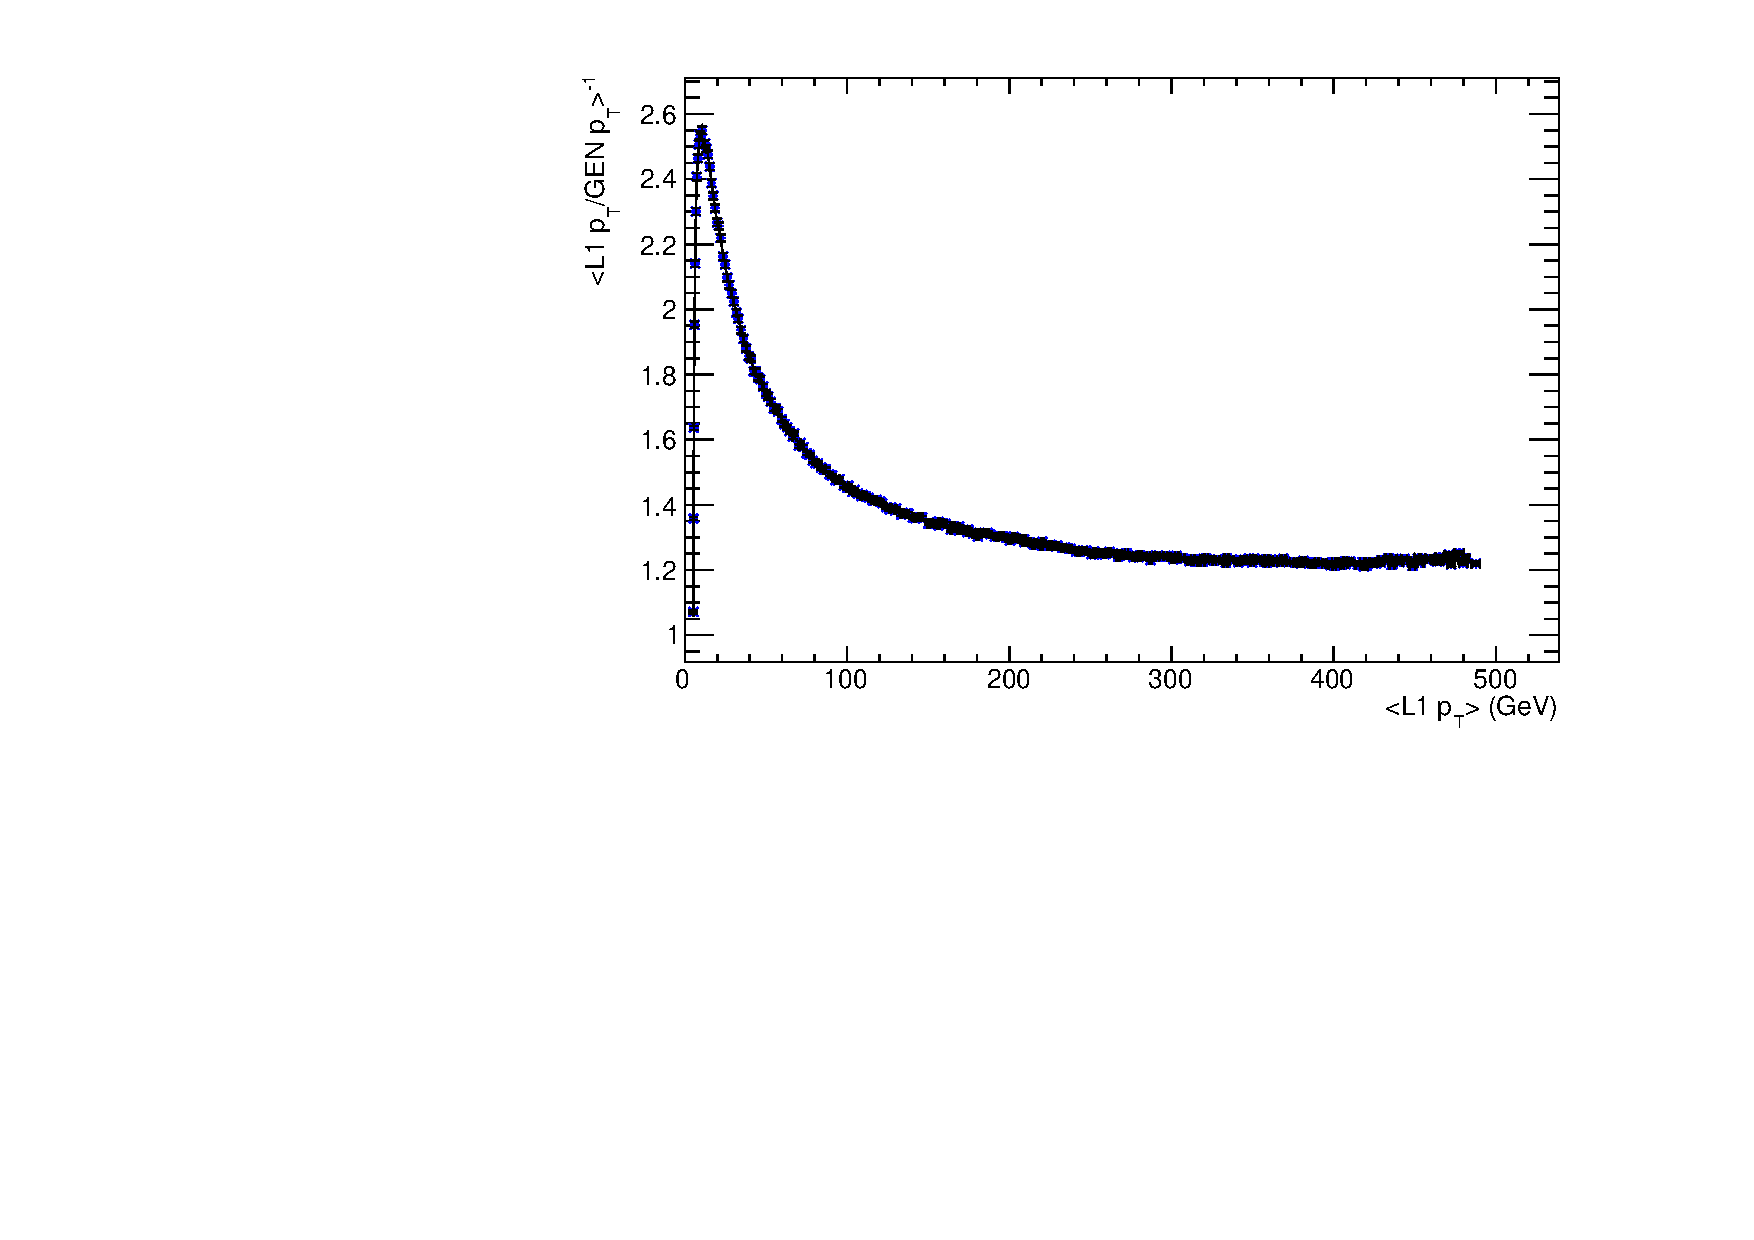
\includegraphics[width=0.5\textwidth]{figs/trigger/p1}
  }~ 
  \subfloat[$0.75<\eta<1.50$]{
    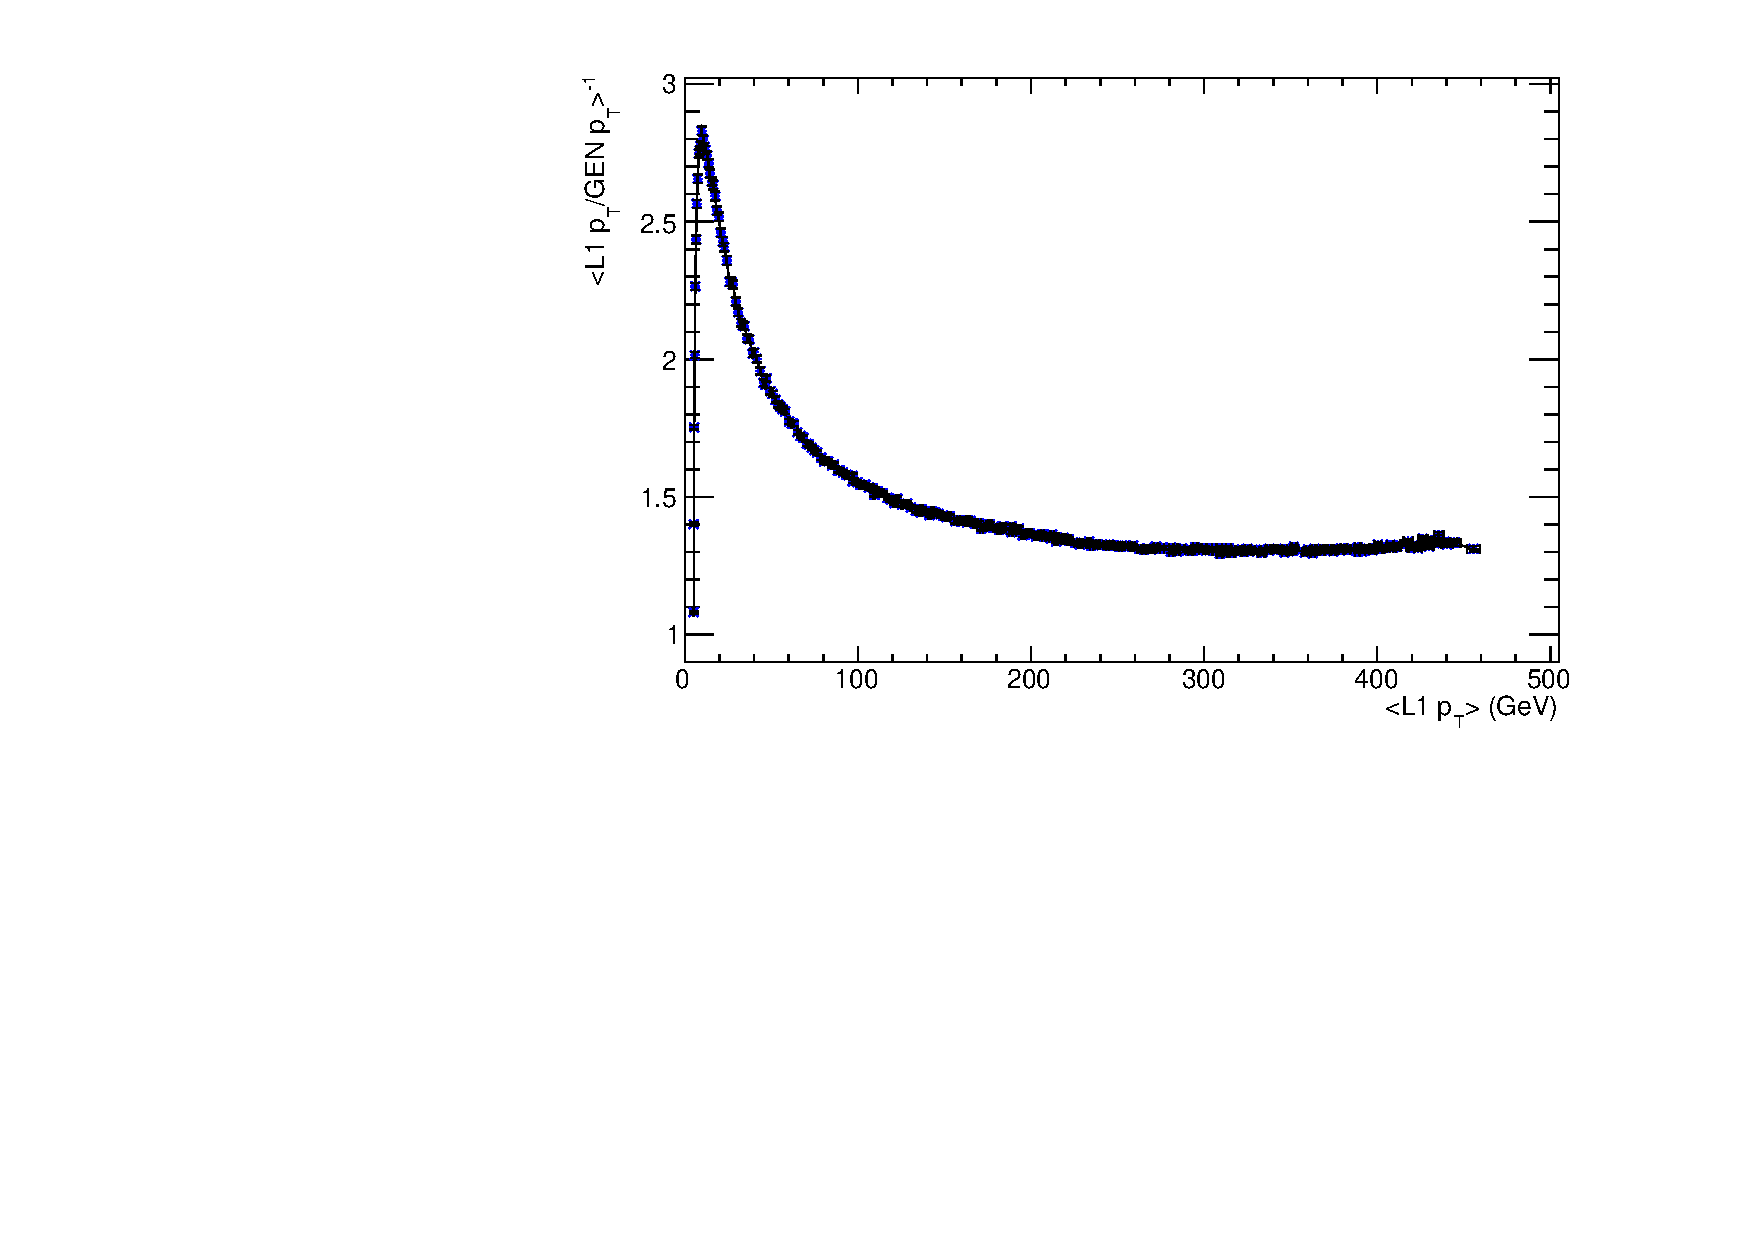
\includegraphics[width=0.5\textwidth]{figs/trigger/p2}
  }\\
  \subfloat[$1.50<\eta<2.25$]{
    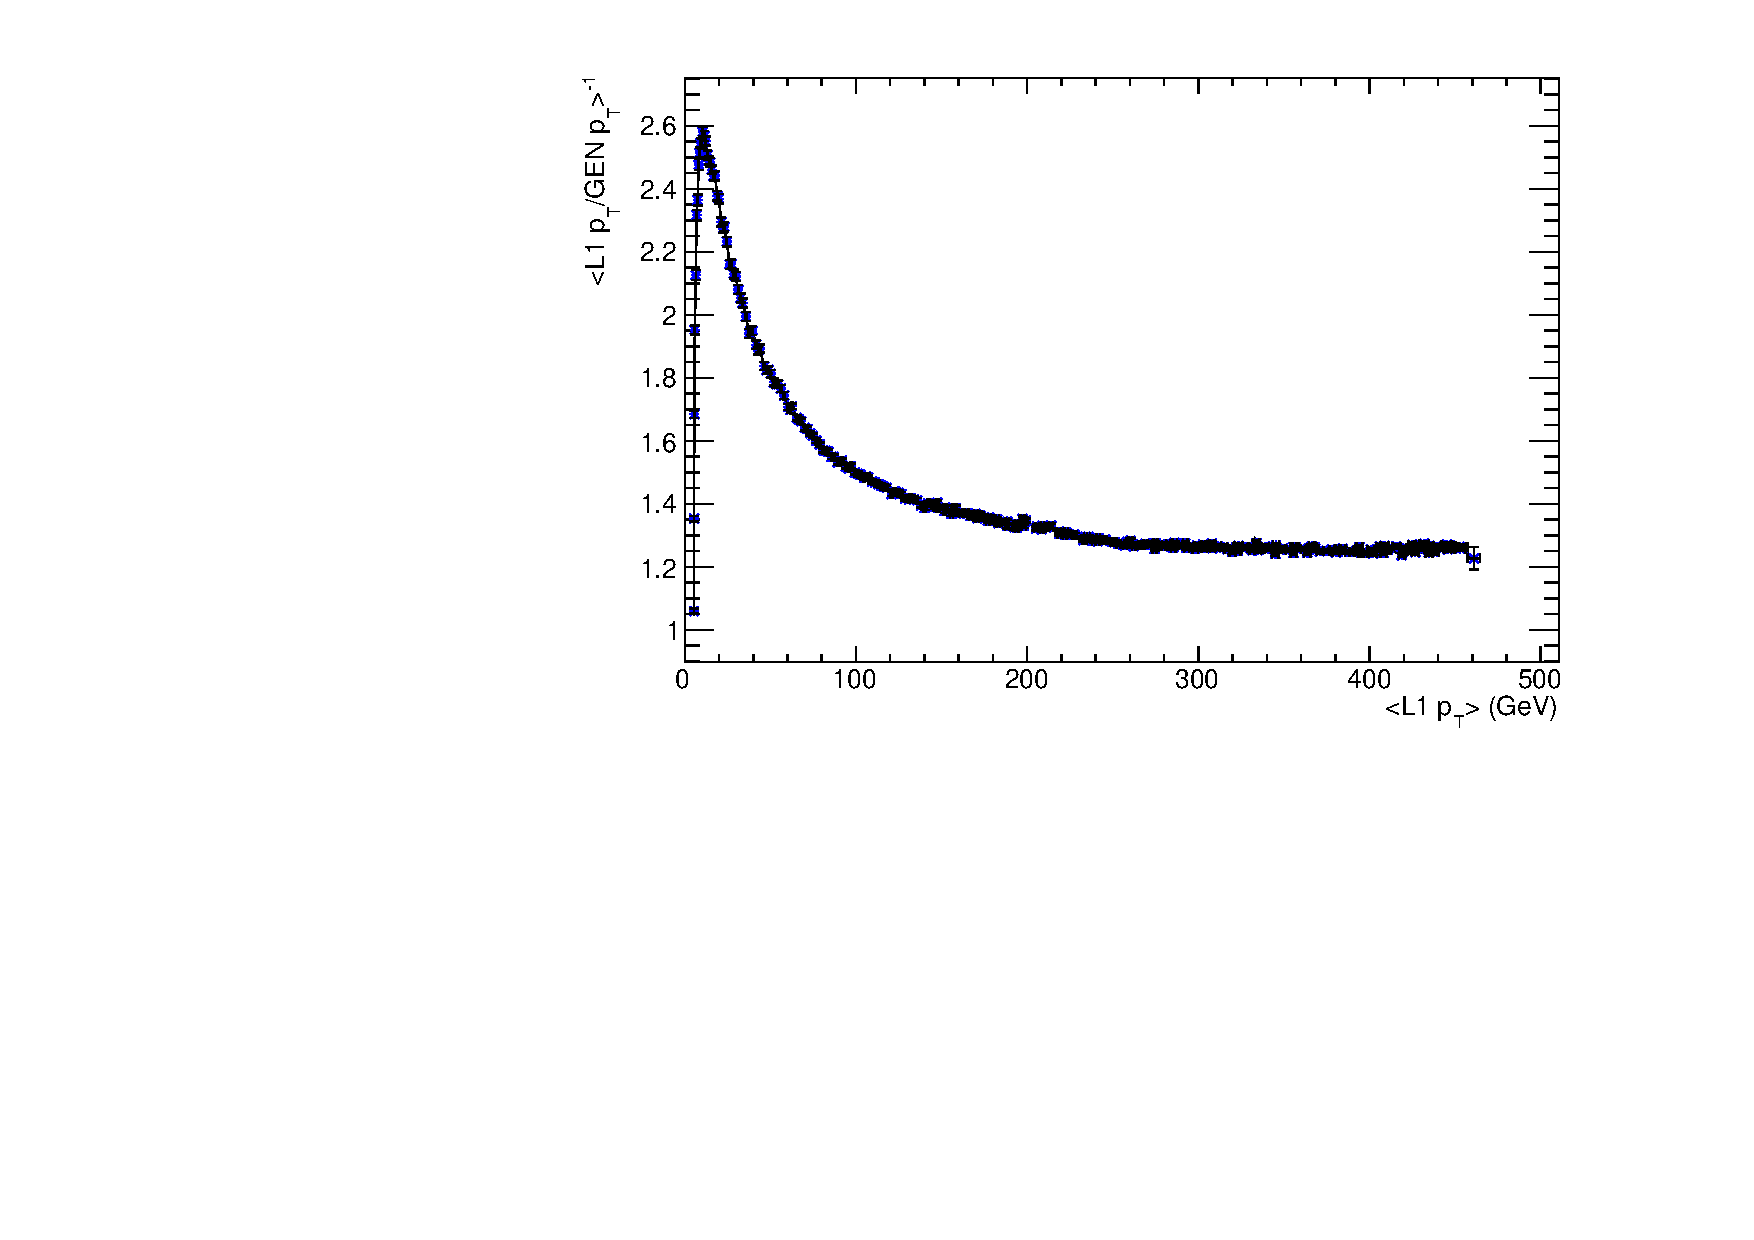
\includegraphics[width=0.5\textwidth]{figs/trigger/p3}
  }~ 
  \subfloat[$2.25<\eta<3.00$]{
    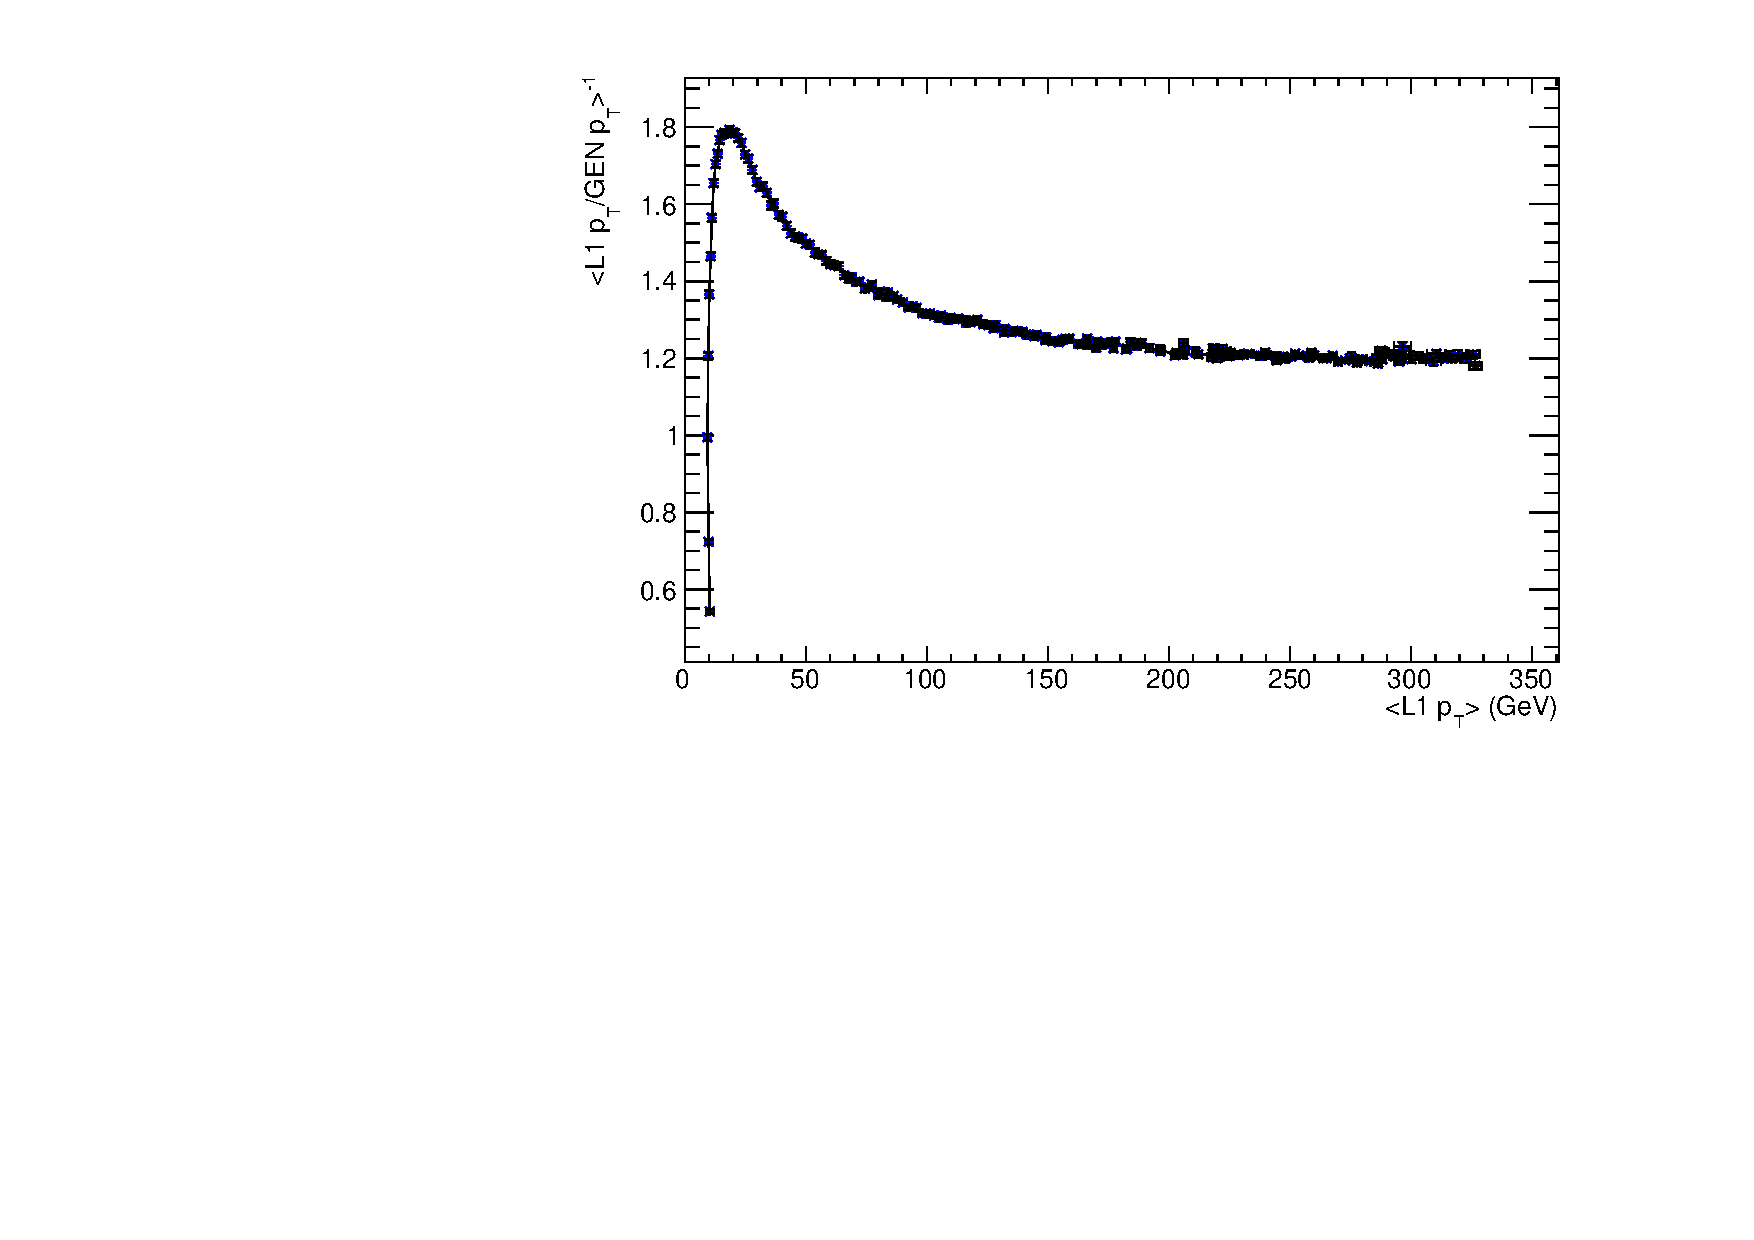
\includegraphics[width=0.5\textwidth]{figs/trigger/p4}
  }\\
  \subfloat[$-0.75<\eta<0.00$]{
    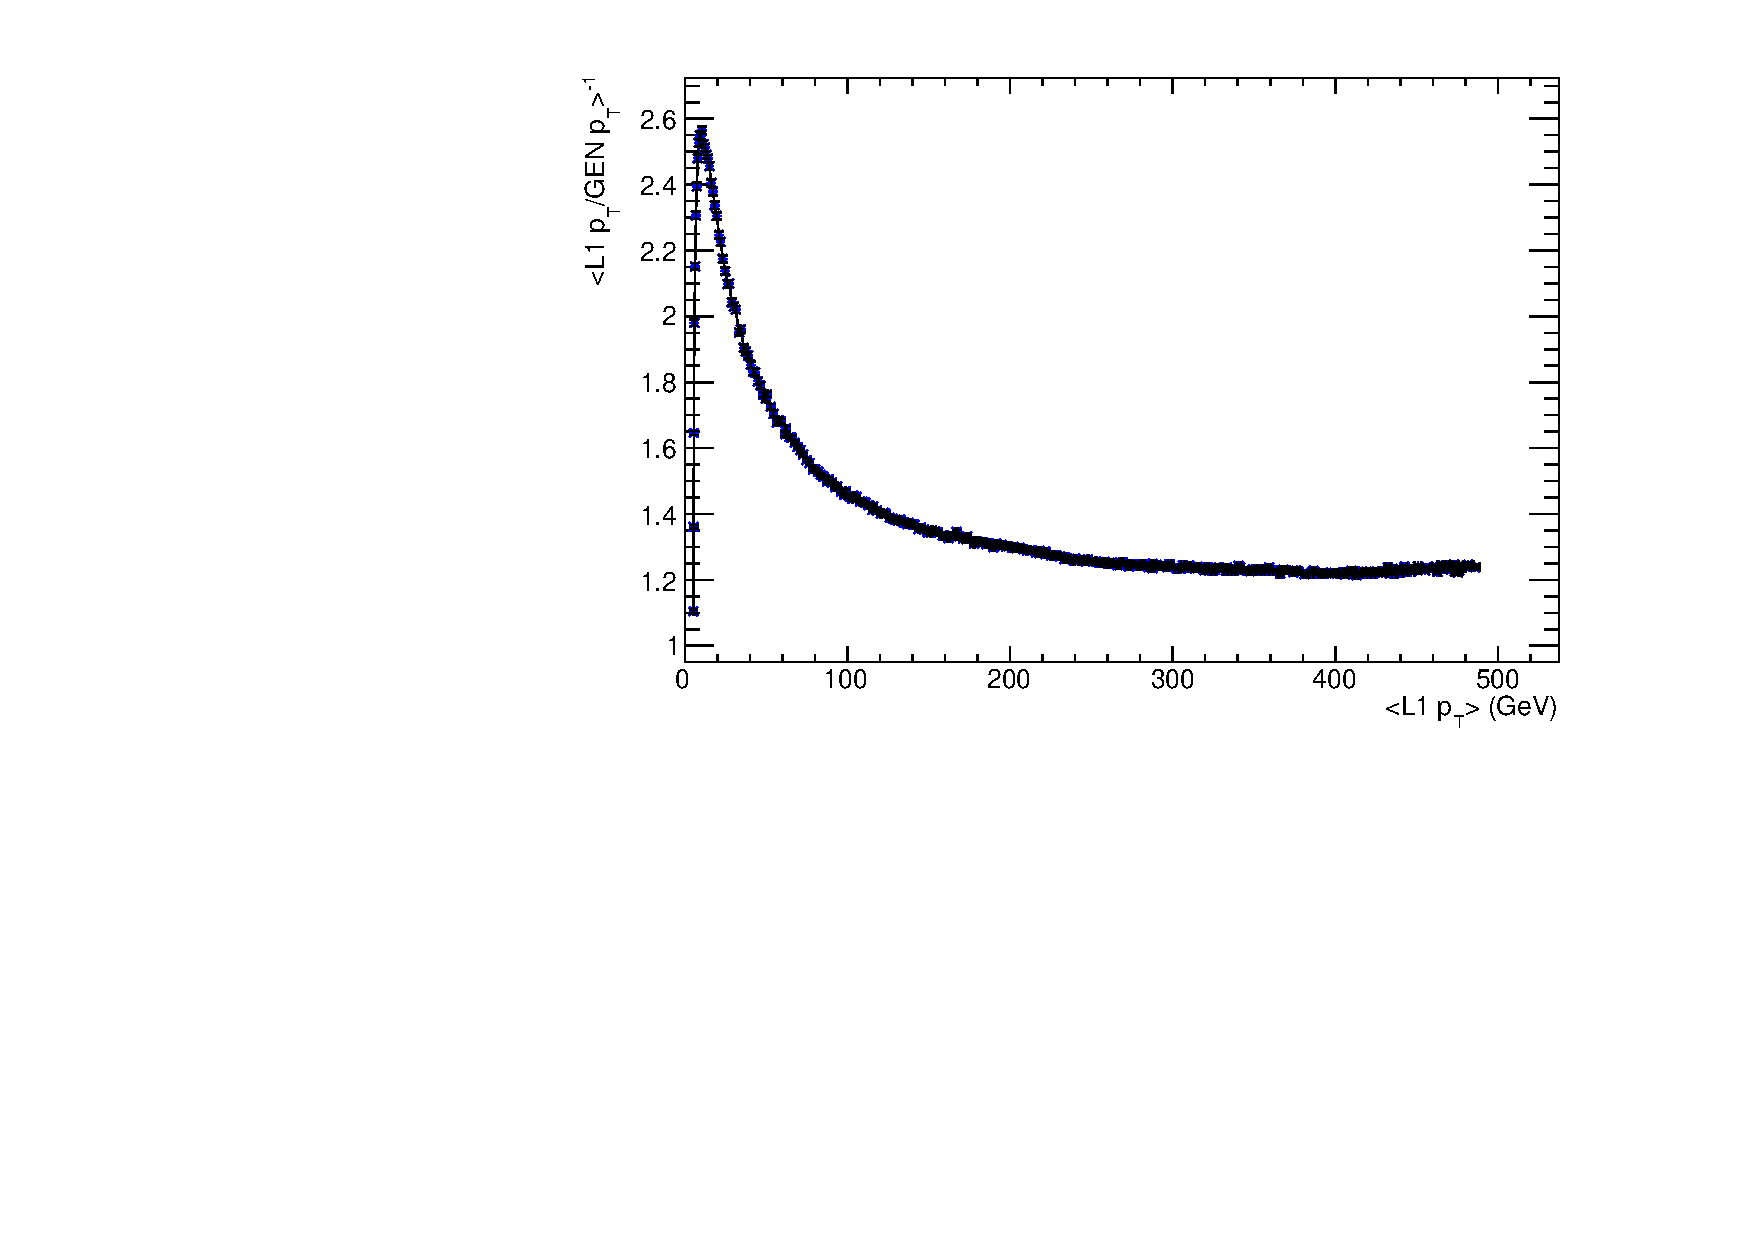
\includegraphics[width=0.5\textwidth]{figs/trigger/m1}
  }~ 
  \subfloat[$-1.50<\eta<-0.75$]{
    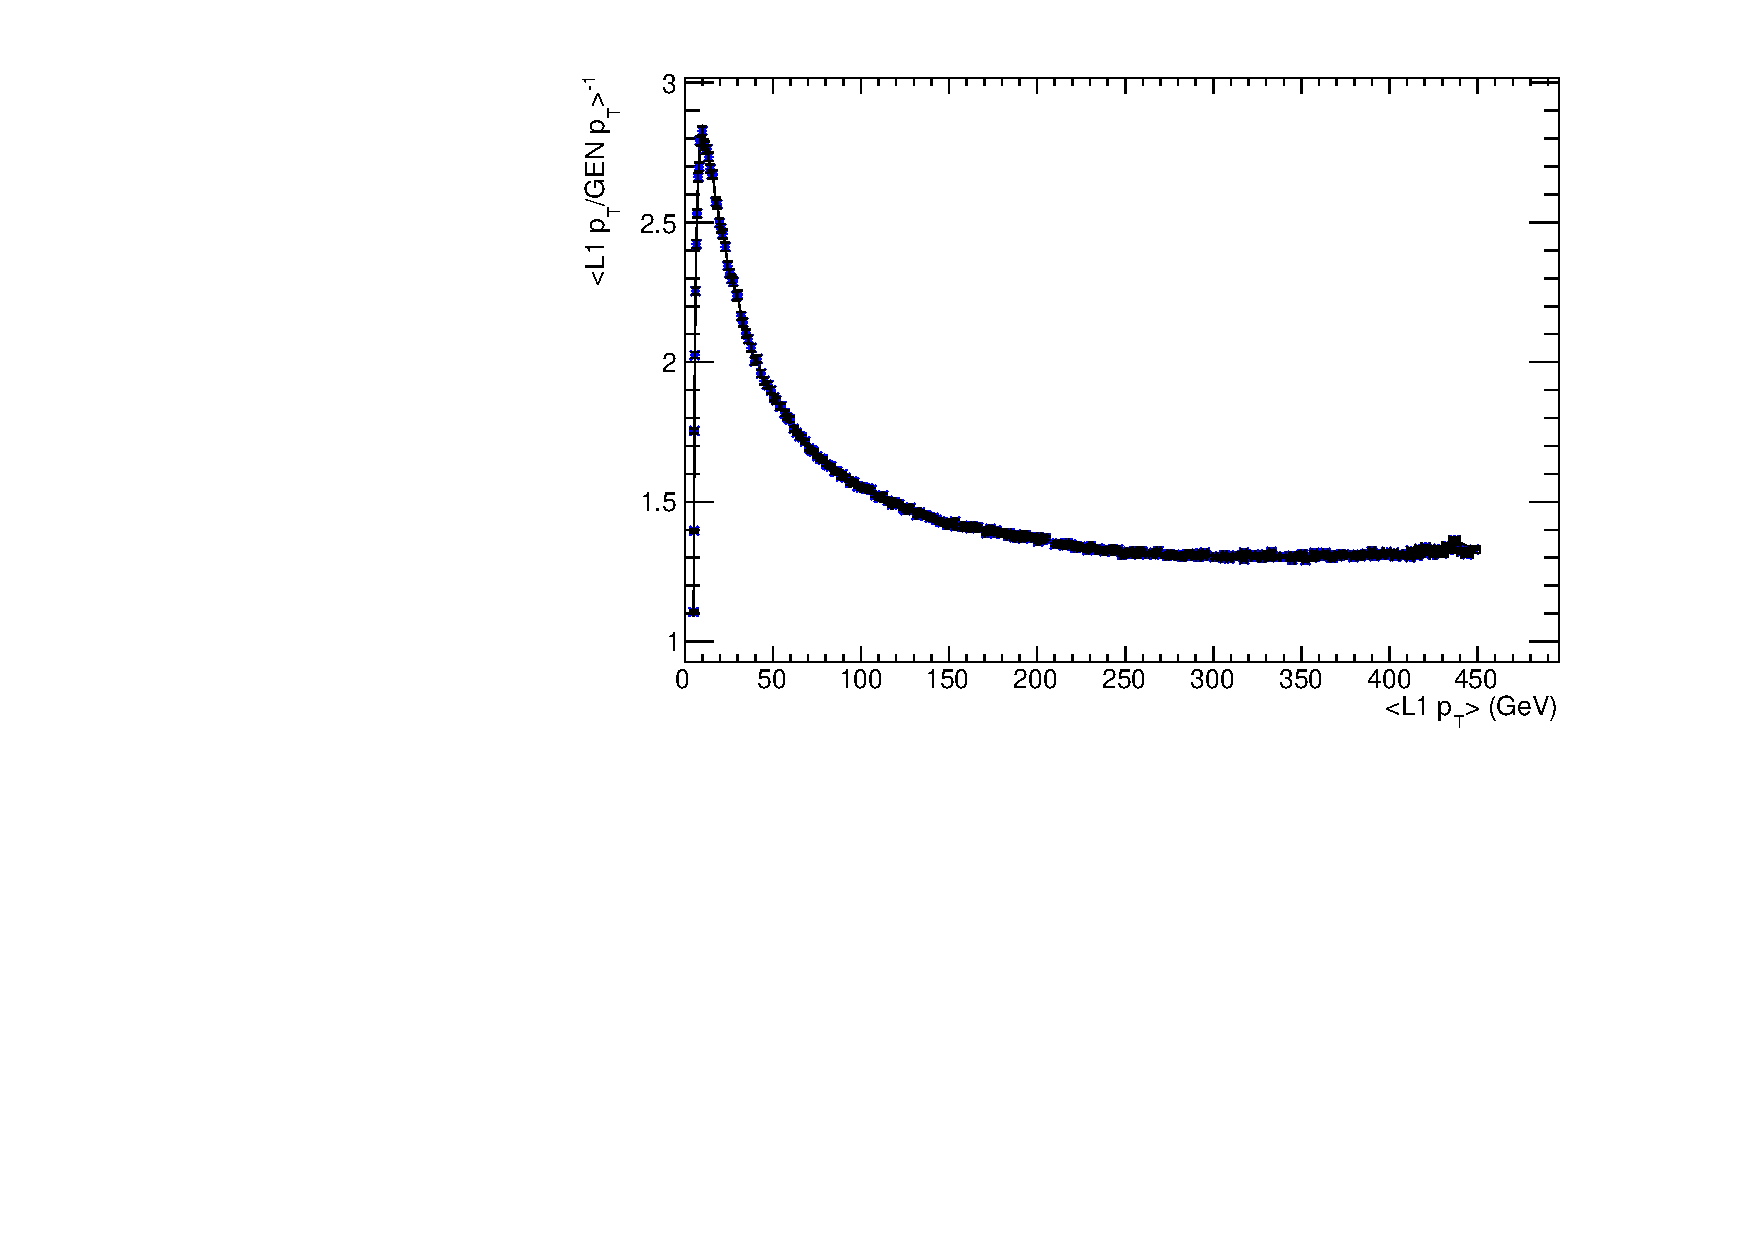
\includegraphics[width=0.5\textwidth]{figs/trigger/m2}
  }\\
  \subfloat[$-2.25<\eta<-1.50$]{
    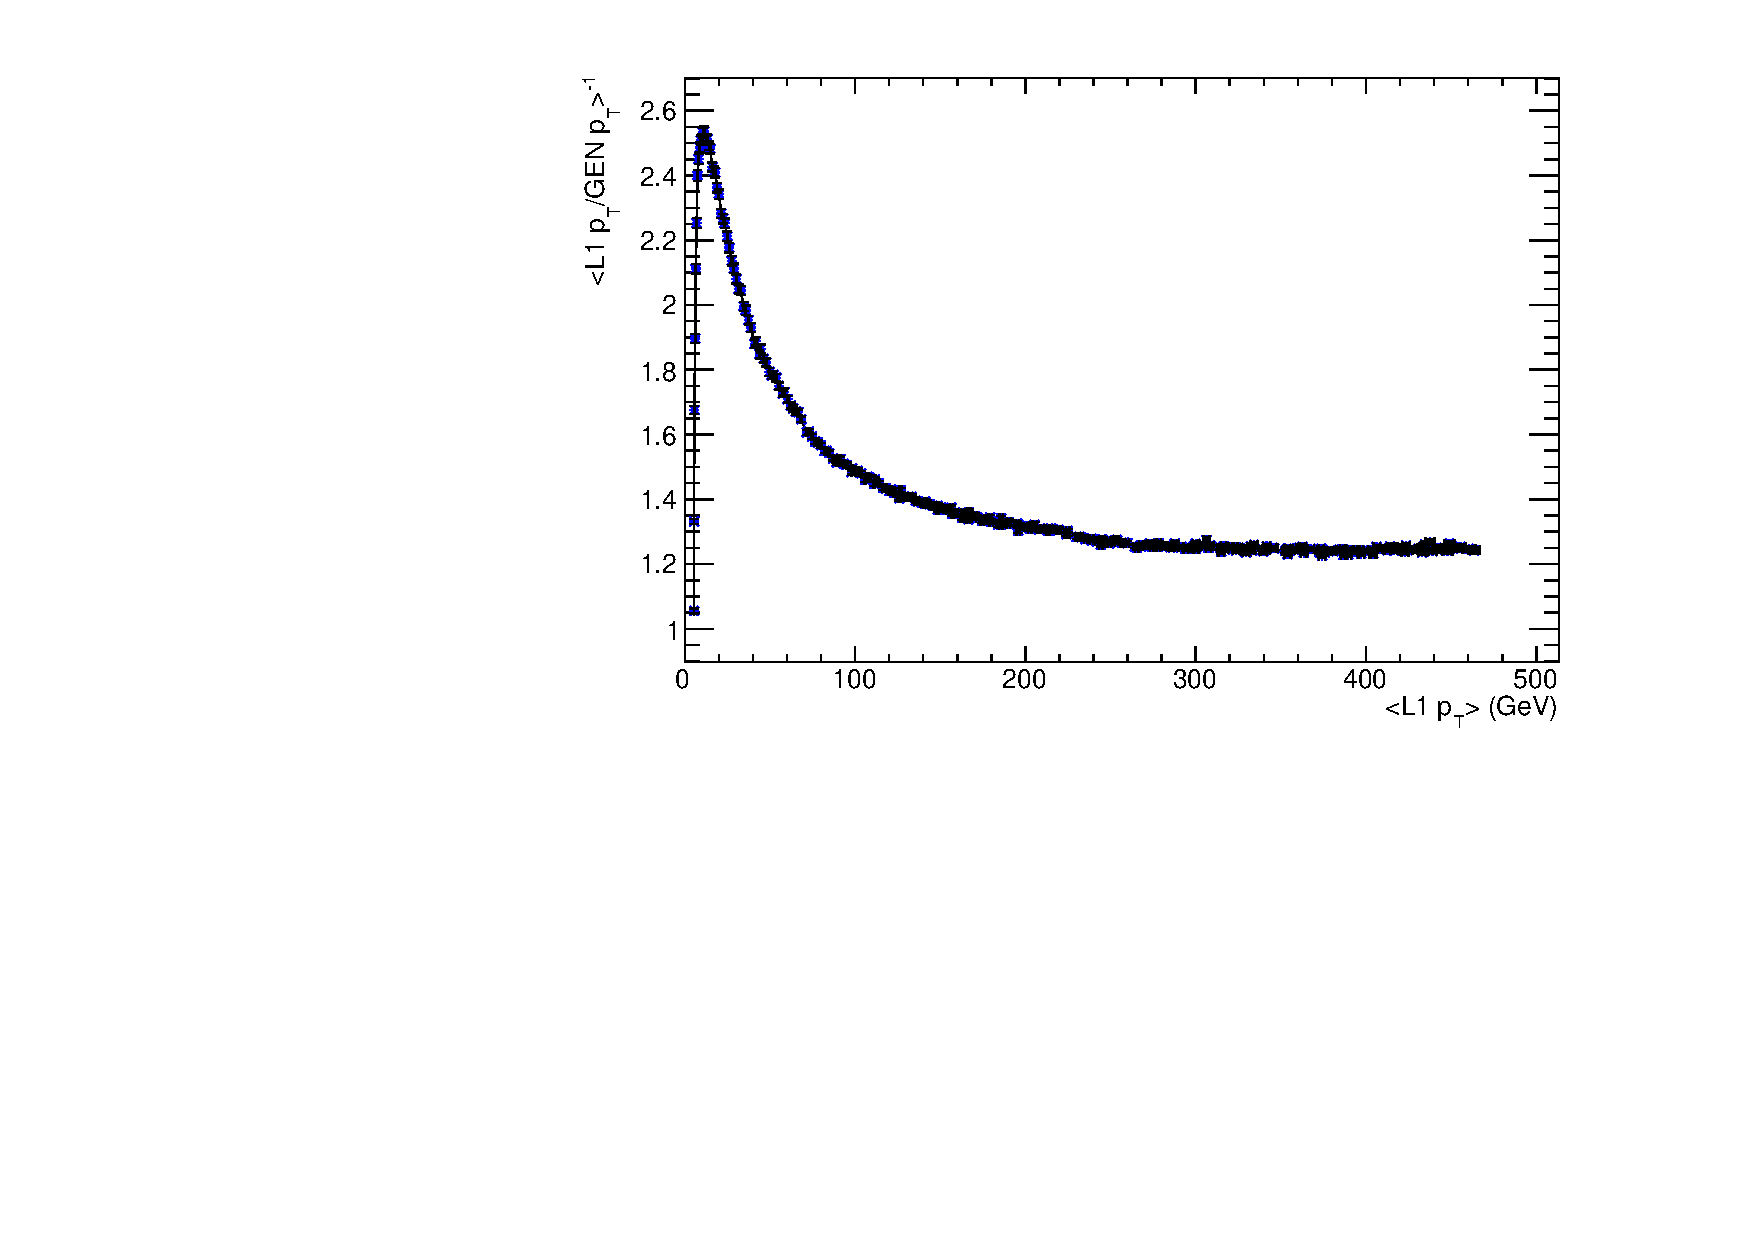
\includegraphics[width=0.5\textwidth]{figs/trigger/m3}
  }~ 
  \subfloat[$-3.00<\eta<-2.25$]{
    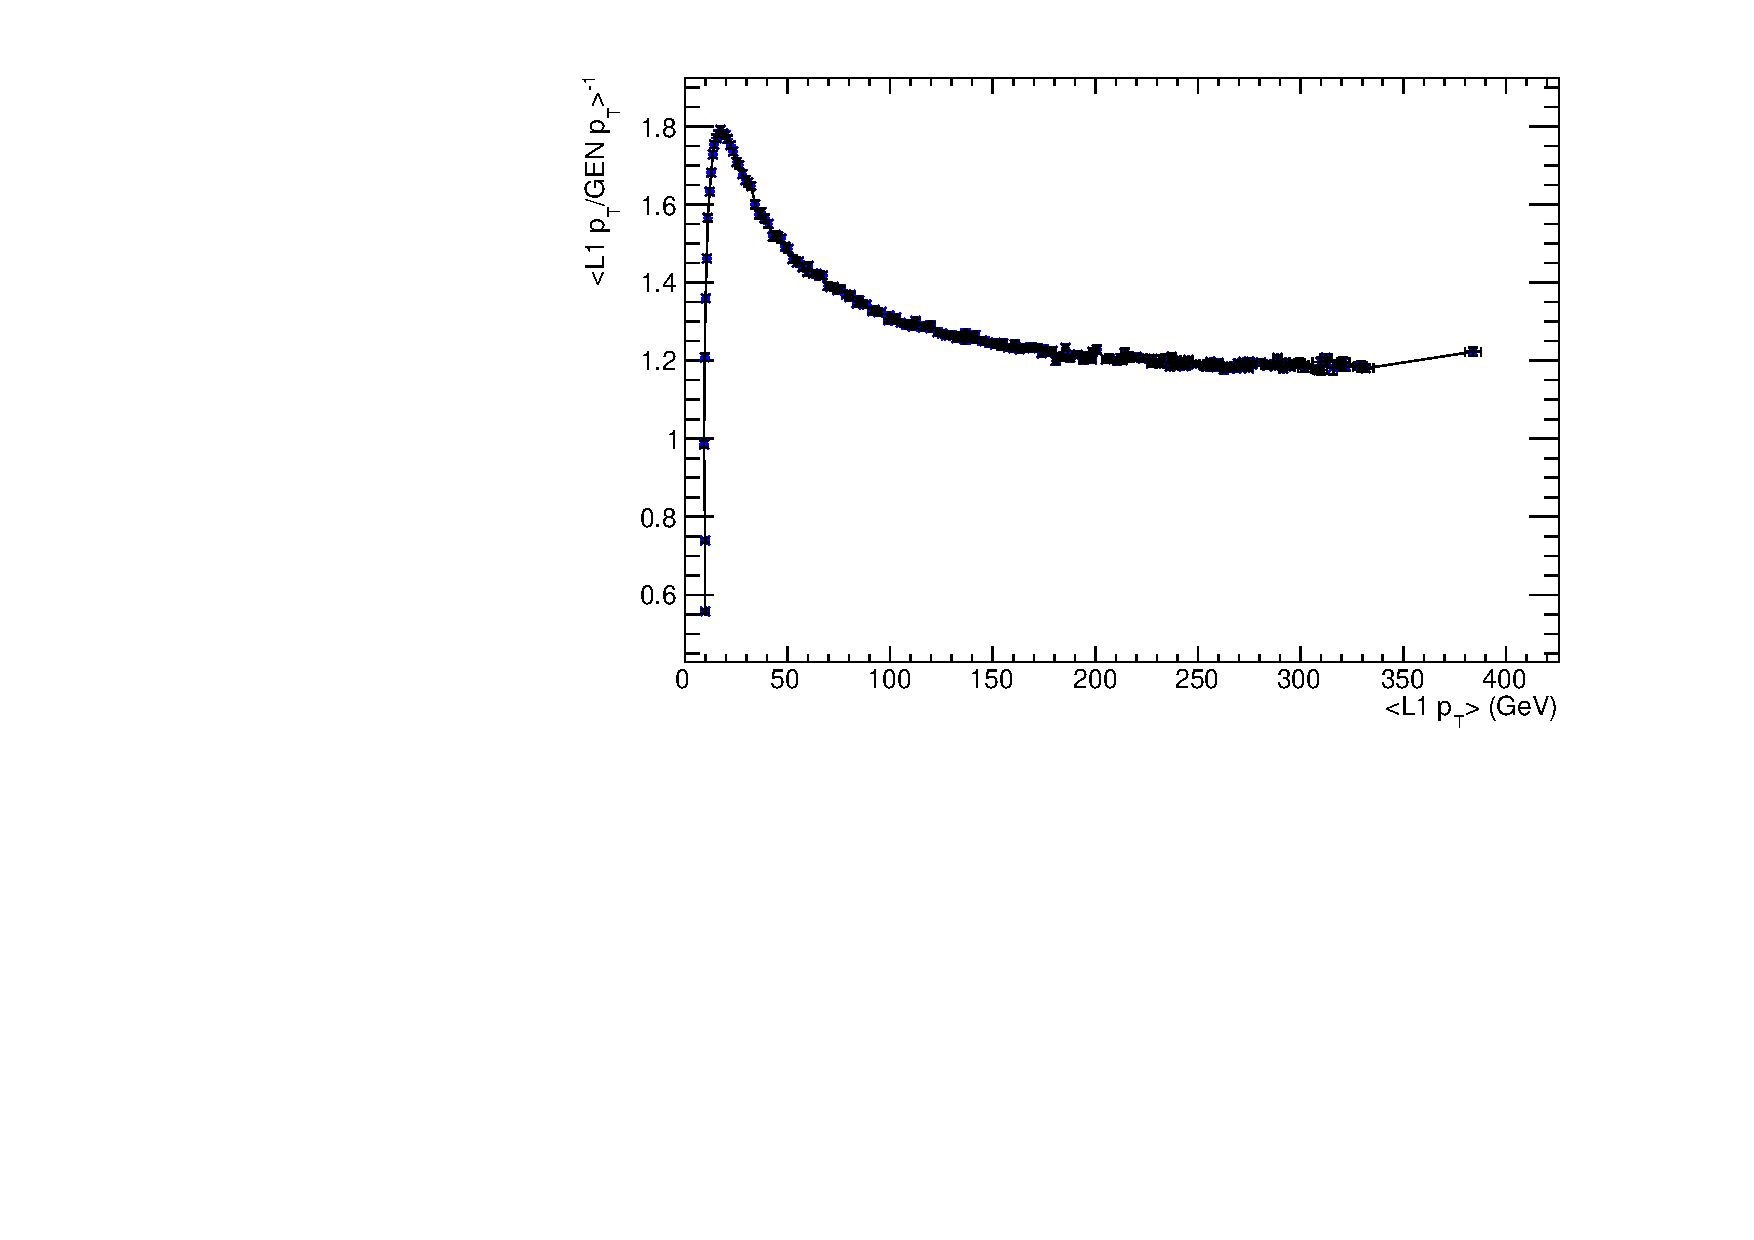
\includegraphics[width=0.5\textwidth]{figs/trigger/m4}
  }
  \caption{Calibration fits across all \eta ranges as a function of
  Level-1 jet \pT}
  \label{fig:calibFunctions}
\end{figure}

To test the calibration procedure a closure test is performed by
applying the calibration function to the simulation that was
used to derive it. The mean response as a function of generator jet
\pT in the range  $|\eta|<1.4$ is shown in
Fig.~\ref{fig:calibclosure} as an example. The
calibration procedure produces a flat response at unity for jets with
$\pT>50~\gev$. Below this value the matching procedure starts to
break-down, as low \pT Level-1 jets are less likely to be matched to a
corresponding generator jet. The Level-1 jets that are matched to a
generator jet are more likely to have a higher value of $\pT$, as
higher $\pT$ jets are more likely to be identified. This skews the
response upwards as the closure test approaches low values of $\pT$.
From observing a series of such closure tests it was concluded that it
was reasonable to consider Level-1 jets with a $\pT>20~\gev$, as in
this case the corrected response was reasonably compatible with unity.

\begin{figure}
	\begin{center}
		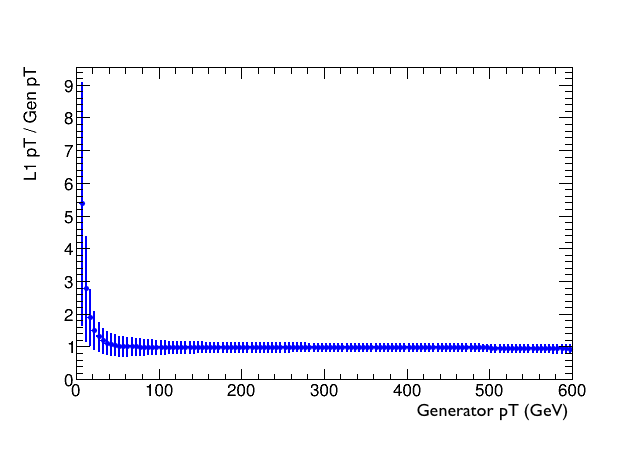
\includegraphics[width=0.8\linewidth]{figs/trigger/calibClosure_s5_donut}
  \caption{Closure test of the calibration procedure, checking the
  response as a function of generator jet \pT in the $|\eta|<1.4$ range.}
  \label{fig:calibclosure}
	\end{center}
\end{figure}

In future upgrades of the \LHC it is proposed to increase the \PU to
$\sim 140$. This will provide a much higher instantaneous luminosity,
but presents a significant challenge for reconstruction. To help
inform this upgrade, the Level-1 jets were produced and calibrated on a
sample with an average \PU of 140. The resulting jet response as a
function of generator jet \pT and Level-1 jet \eta can be seen in
Fig.~\ref{fig:pu140calibclosure}. The calibration was performed on
jets with a seed of 2.5~\gev and chunky donut subtraction. The
response is within $10\%$ of unity up to $|\eta|<2.5$ and for Level-1
jets with $\pT>50~\gev$. This suggests that the calibration and \PUS
procedure scales reasonably well with the number of \PU interactions.

\begin{figure}
	\begin{center}
		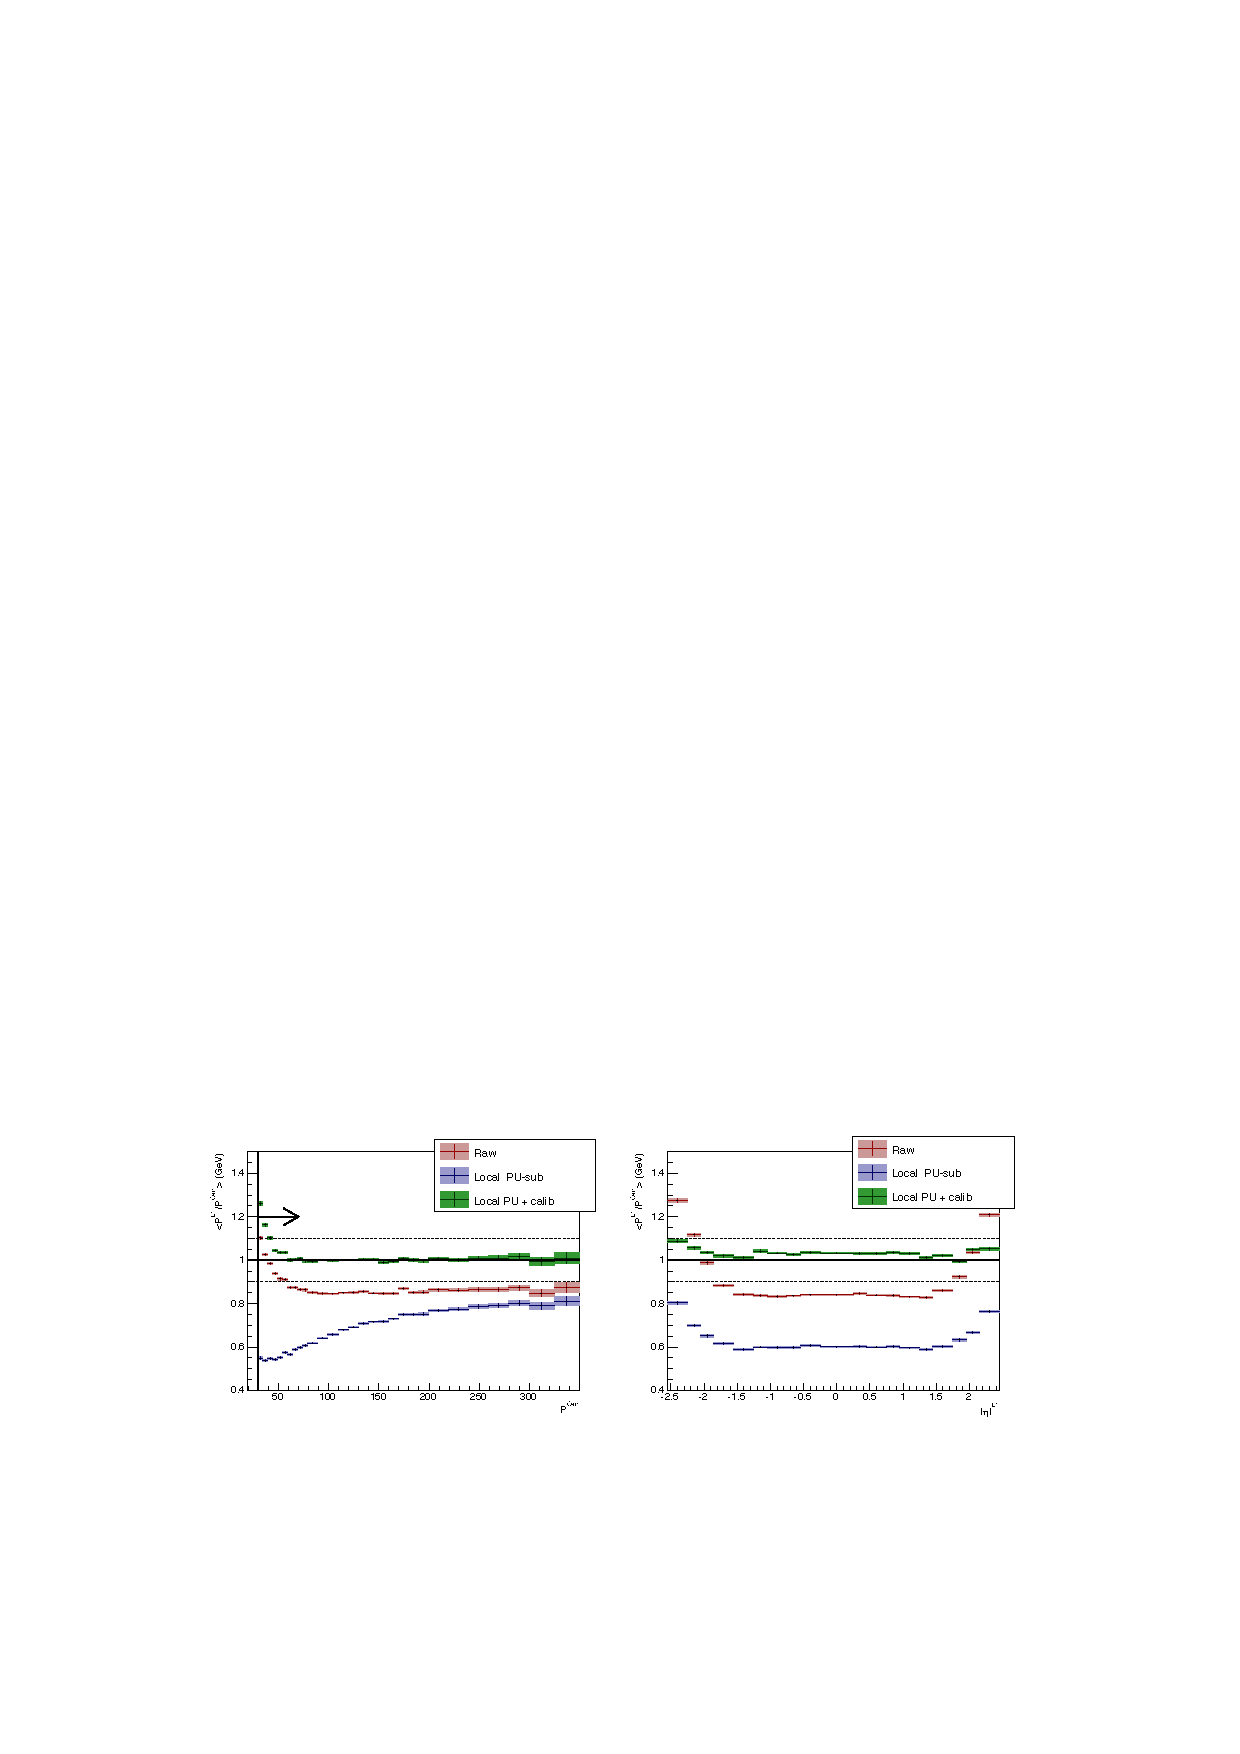
\includegraphics[width=1.0\linewidth]{figs/trigger/pu140_calib_closure}
  \caption{The ratio of the \pT of Level-1 jets with matched generator
  jets before and after they are calibrated. This is carried out at a
  \PU of 140 and, demonstrates the effectiveness of the calibration in
  these extreme conditions.}
  \label{fig:pu140calibclosure}
	\end{center}
\end{figure}

\section{Performance of the upgraded algorithm}

\label{sec:jet_algo_performance}

The performance of the jet algorithm with the various methods of \PUS 
described in Sec.~\ref{sec:pus} is tested on 13~TeV \MC simulation with an
average \PU of 40. A comparison is made to the jets produced by the
\GCT as it was in 2012. In some cases the performance of the interim
calorimeter trigger that was run in the early stage of 2015 during the
commissioning of the upgraded trigger is plotted with label
\emph{UCT}. To investigate rates a minimum bias sample was used, this
sample only consists of overlaid \PU events and has no generator jets.
To test physics performance a sample of simulated $t\bar{t}$
events was used, which contains generator jets that originate from
the hard interaction. The Level-1 jets are calibrated for each
type of \PUS with the method as outlined in Section~\ref{sec:l1jec}.

Fig.~\ref{fig:matchingeff} shows the efficiency of generator jets,
produced as described in Sec.~\ref{sec:l1jec}, being matched to a
Level-1 jet as a function of their $p_T$. If a generator jet has a
corresponding Level-1 jet within a radius $R=0.5$ it is counted as
matched.
This radius is chosen as the distance from the centre of a L1 jet to
the corner of its $9\times9$ square. A representative selection of the
different \PUS algorithms are shown. All of the upgrade Level-1 jet
algorithms have close to $100\%$ efficiency above $70$~GeV. The
application of a seed threshold significantly reduces the efficiency
for low $p_T$ jets, but the donut subtraction does not remove any
extra signal jets.
%Checked matching to gen, dr 32, inefficiencies caused by algorithm - gct bad
\begin{figure}
	\begin{center}
		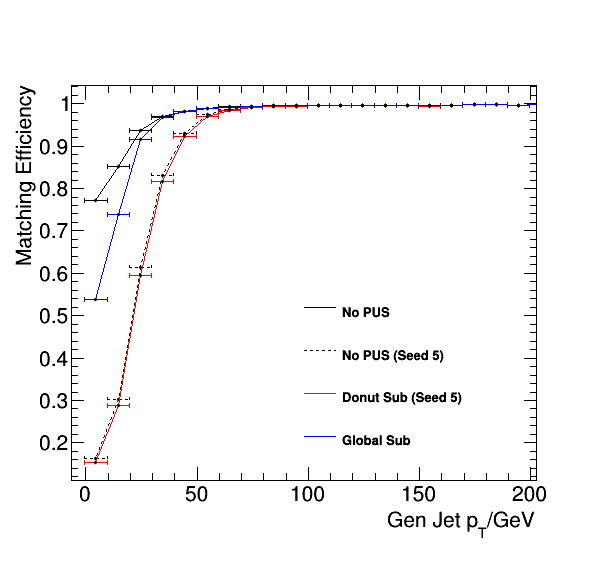
\includegraphics[width=0.6\linewidth]{figs/trigger/performance/matchingeff_alljet}
	\end{center}
	\caption{The efficiency with which a generator jet has a
  corresponding L1 jet within a radius, $R=0.5$. This is carried out
  for all Gen jets in 70~000 simulated $t\bar{t}$ production events.}
	\label{fig:matchingeff}
\end{figure}

A key goal of \PUS is to reduce the dependence of the Level-1 trigger
acceptance rate on the number of \PU interactions. To quantify this
for a representative selection of algorithms, the rate against the
number of reconstructed vertices is plotted for the minimum bias sample,
Fig.~\ref{fig:ratenvtx}. The rate is defined as the fraction of
minimum bias events that pass a Level-1 jet $p_T$ cut of $30$~\gev.
This cut is applied to a different jet rank depending on the type of
trigger to be tested. For the \emph{single-jet} trigger the cut is applied to
the lead jet, for a \emph{quad-jet} trigger the cut is applied to the
fourth leading jet. The different forms of \PUS clearly reduce the
dependence of the rate on the number of interactions. The upgrade algorithm
performs significantly better than the \GCT, where the jet trigger
rates are incredibly sensitive to PU. Of the algorithms investigated,
the seed of 2.5~\gev, denoted \emph{Seed 5}, has the most dramatic
effect due to its ability to kill soft \PU jets. The \rho-area
subtraction, denoted \emph{Global Sub}, also performs well. Applying
donut subtraction without a seed threshold does not make much difference for this
particular \PUS benchmark. This is likely due to the fact that
donut subtraction works well in correcting the resolution of jets
contaminated with soft particles from \PU vertices, rather than
removing low \pT jets that originate from \PU.

\begin{figure}
  \centering
  \subfloat[Single-jet trigger $\pT>30~\gev$]{
    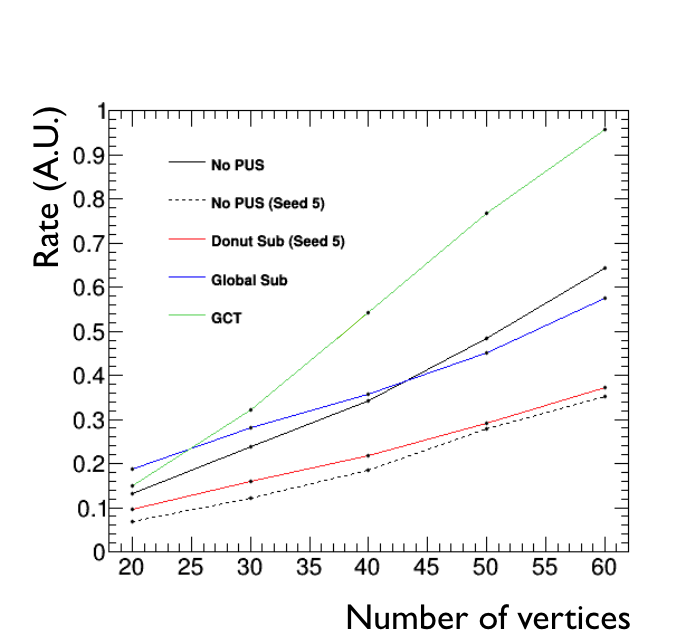
\includegraphics[width=0.5\textwidth]{figs/trigger/performance/rateNVertLeadJet}
  }~ 
  \subfloat[Quad-jet trigger $\pT>30~\gev$]{
    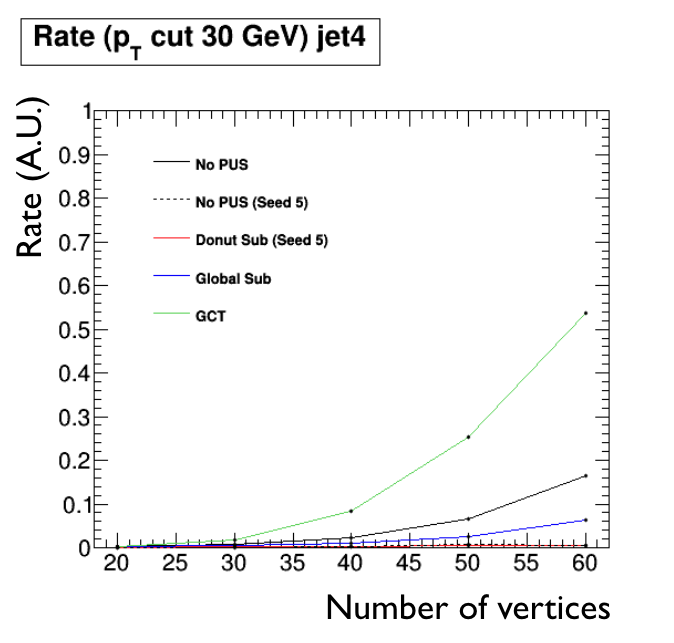
\includegraphics[width=0.5\textwidth]{figs/trigger/performance/rateNVertFourthJet}
  }
  \caption{The relative rate of events with $p_T>30$~GeV leading (a)
  and fourth leading (b) jets after different \PUS algorithms with and
  without seed thresholds for $70 000$ zero bias events as a function
  of the number of reconstructed vertices.}
  \label{fig:ratenvtx}
\end{figure}

To characterise the energy resolution of the Level-1 jets with
different \PUS algorithms, the efficiency turn-on curves are plotted
in Fig.~\ref{fig:turnons}. The lead jet efficiency turn-on,
Fig.~\ref{fig:leadJetTurnon}, is
made by matching the generator jets to Level-1 jets, requiring $\Delta
R<0.5$ and taking the ratio of the matched generator jet $p_T$
distribution without a cut on the Level-1 jet with the matched
generator jet distribution after a cut on the Level-1 jets. Most algorithms
show a similar performance for a single-jet trigger. The effects of
\PU are less relevant when just considering one high energy object.

More difference is observed when all jets with $\pT>20~\gev$ are
summed to find the Level-1 $\HT$ of the event. The plot in
Fig.~\ref{fig:htTurnon} is made by taking the ratio of generator $\HT$
(also made from 20~\gev jets), with and without a cut on the Level-1
\HT. When considering a scalar sum of jets the effects of pileup
add up and the different algorithms have a more significant
separation. It is clear that performing \PUS helps to significantly
improve the energy resolution of Level-1 $\HT$.
\begin{figure}
  \centering
  \subfloat[Lead jet $p_T^{L1}>150~\gev$ efficiency]{
    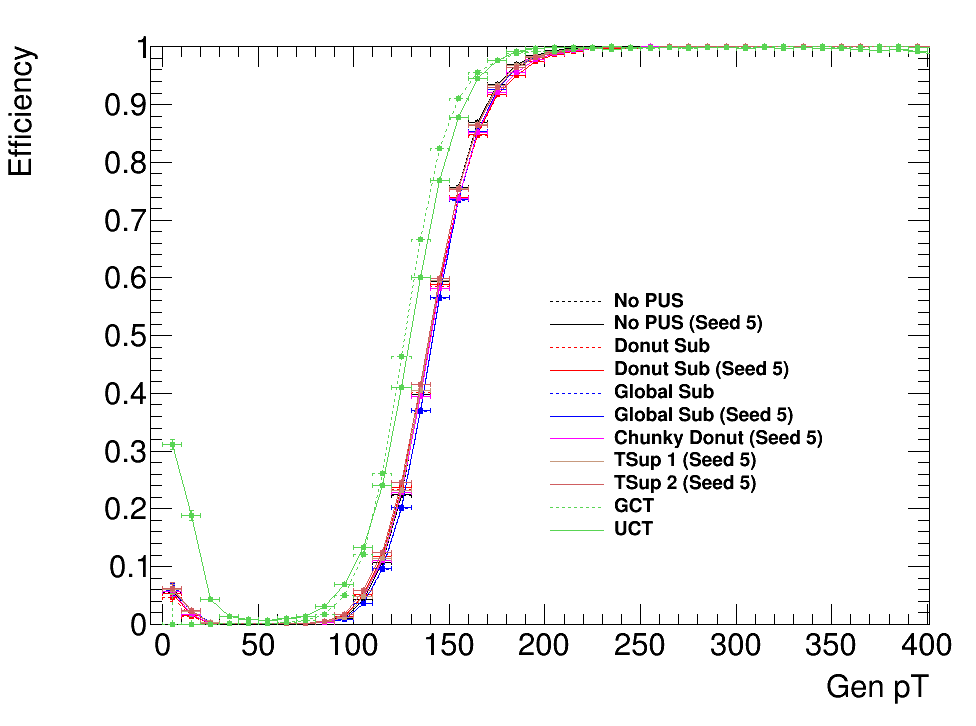
\includegraphics[width=0.515\textwidth]{figs/trigger/performance/leadJet_150_turnon}
    \label{fig:leadJetTurnon}
  }~
  \subfloat[$\HT^{L1}>200~\gev$ efficiency]{
    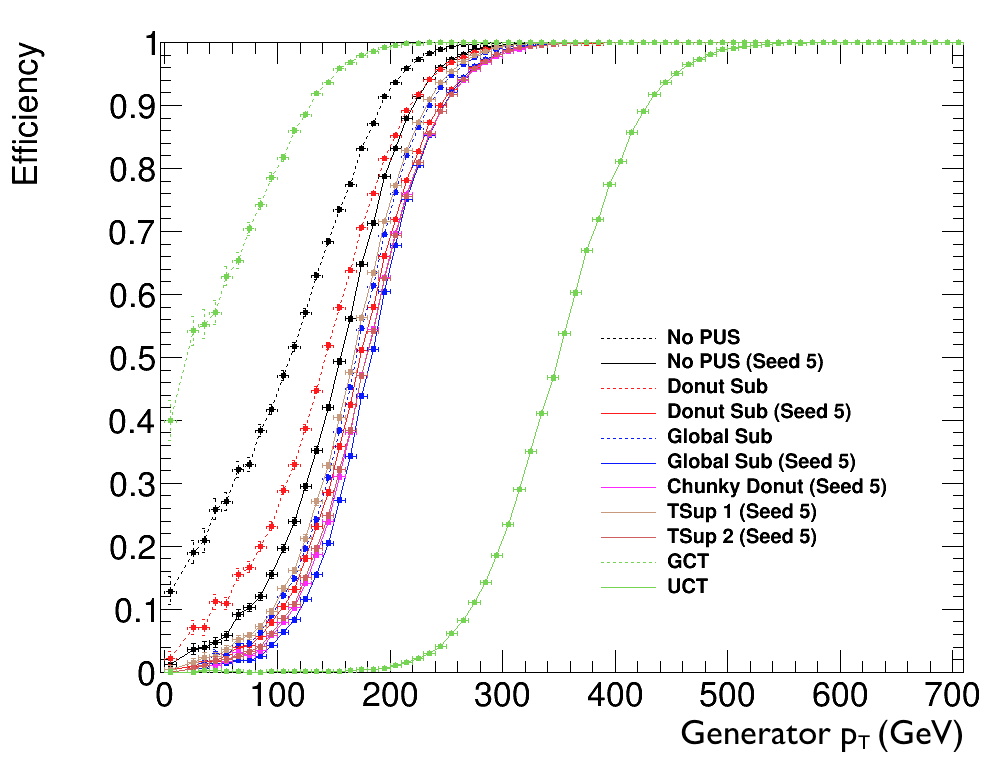
\includegraphics[width=0.485\textwidth]{figs/trigger/performance/ht_200_turnon}
    \label{fig:htTurnon}
  }
  \caption{ Efficiency after a specific cut for Level-1 leading jets (a) and Level-1 \HT
  (b) as a function of the corresponding generator quantity.
  } \label{fig:turnons}
\end{figure}

In the turn-on curves, a change in offset along the $x$-axis results
from a difference in jet energy scale with respect to the generator
quantity. As the \GCT jets do not have any calibration applied and the
UCT has a different type of calibration, this can differ
significantly. However, this does not give all the relevant
information when deciding on a final algorithm to increase the overall
performance of the trigger. The most important consideration is the
trade-off between the efficiency of the algorithm at picking out a
particular physics signature for a given rate. This does not depend on
the specific energy scale of the jets relative to the generator
quantities.

To better characterise the different Level-1 jet algorithms independently of energy
scale, the efficiency of selecting events with a particular generator
level jet quantity is plotted against the rate from a minimum bias
sample. In each case, a range of thresholds for the equivalent Level-1
quantity are scanned through and the rate and efficiency for the
thresholds are plotted. The rate is calculated for an instantaneous luminosity
of $7\times10^{33}$~cm$^{-2}$s$^{-1}$ with a 50~ns \LHC bunch crossing
interval. Figure~\ref{fig:rateEffJet} shows the rate of the Level-1
trigger in Hz against the efficiency of selecting events for jet
triggers. In Fig.~\ref{fig:leadJetRateEff} the efficiency of
selecting $t\bar{t}$ events containing a generator jet with
$\pT>150~\gev$ is plotted against the minimum bias rate for an
equivalent Level-1 threshold. The rate and efficiency are plotted for
a range of cuts on the lead Level-1 jet for all the jet algorithms
discussed in this chapter. In Fig.~\ref{fig:fourthJetRateEff} the
efficiency of selecting events with a fourth leading generator jet
with $\pT>50~\gev$ are plotted for a range of cuts on the fourth Level-1
jet. As was observed in the turn-on curves, the efficiencies for the
lead jet triggers do not depend so much on the type of \PUS, although
there is a moderate improvement for all the upgrade algorithms over
that used in the \GCT. The difference becomes more evident when
considering the efficiency of selecting a fourth leading jet. The
lower \pT fourth leading jets show a more significant improvement with
the upgraded jet algorithm. The application of \PUS has some effect
but it is still not significant when just considering relatively high
$\pT$ and low multiplicity jets. The performance favours some form of
seed threshold, with the global \PUS performing slightly better than
the local variants.

Considering the jet triggers is important to understand the
behaviour of the upgraded algorithm for individual jets. However,
energy sum triggers are typically more widely used when searching for
signatures of \BSM physics with lots of hadronic activity and missing
energy. This is due to the fact that they give a total measure of the
hadronic energy scale of the event and a strong indication of the
presence of any weakly interacting particles. The performance of the
\HT and \MHT triggers is therefore of significant interest and shown
in Fig.~\ref{fig:rateEffJet}. In Fig.~\ref{fig:htRateEff} the
efficiency of selecting $t\bar{t}$ events with a scalar sum of $p_T>20~\gev$
generator jets that is greater than $200~\gev$ for a range of
thresholds on the Level-1 $\HT$ is plotted against the minimum bias
rate. When many jets are summed in this way the application of \PUS
makes a significant difference. Applying a seed threshold on the
selected jets performs well. Applying the chunky donut or
$\rho$-area \PUS methods on top of a seed threshold obtains the best result.

Figure~\ref{fig:mhtRateEff} shows a similar rate and efficiency curve
for the \MHT variable. For reference on this plot the \MET rate and
efficiency, labelled \emph{MET}, is also shown. As a
vector sum of jets is not made in the interim trigger, the curve with
the UCT label is a form of \MET constructed from \ac{RCT} regions. As \MET
uses the full granularity \TT information without any clustering it
has an improved resolution, but loses robustness as the inputs are not
calibrated and are more susceptible to influence from detector noise.
Of the rate and efficiency curves constructed from a vector sum of
jets, it is again observed that a seed threshold with chunky donut or
\rho-area \PUS give the best performance.

\begin{figure}
  \centering
  \subfloat[Lead jet $p_T>150~\gev$]{
    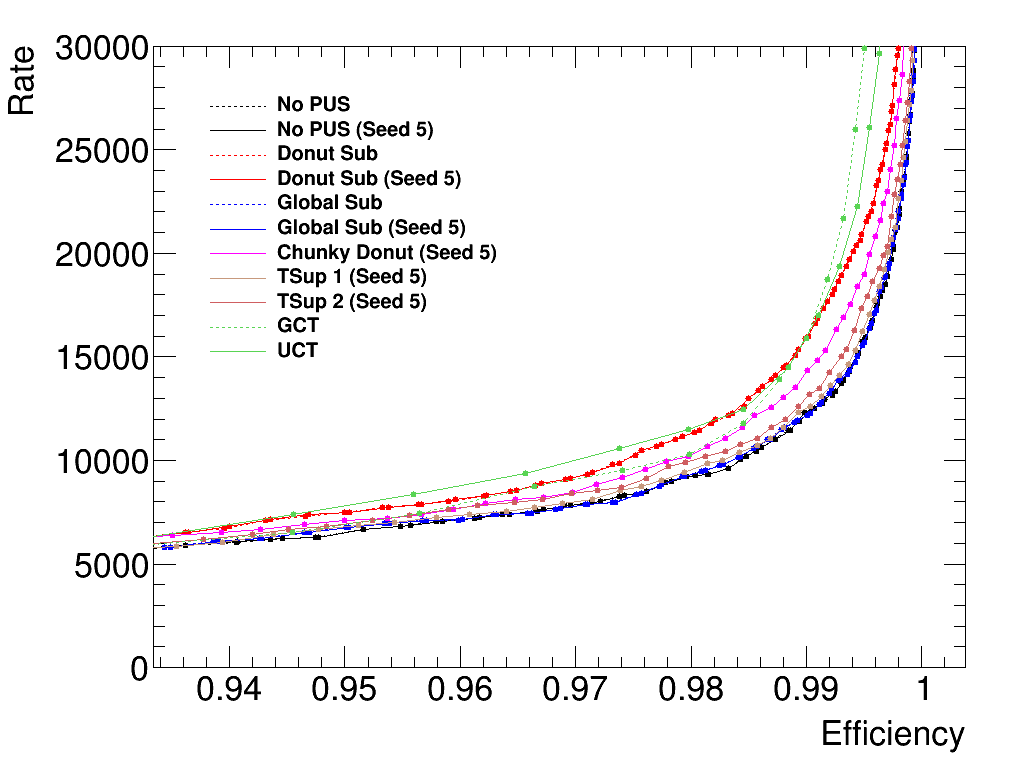
\includegraphics[width=0.48\textwidth]{figs/trigger/performance/singleJet_150}
    \label{fig:leadJetRateEff}
  }~ 
  \subfloat[Fourth leading jet $p_T>50~\gev$]{
    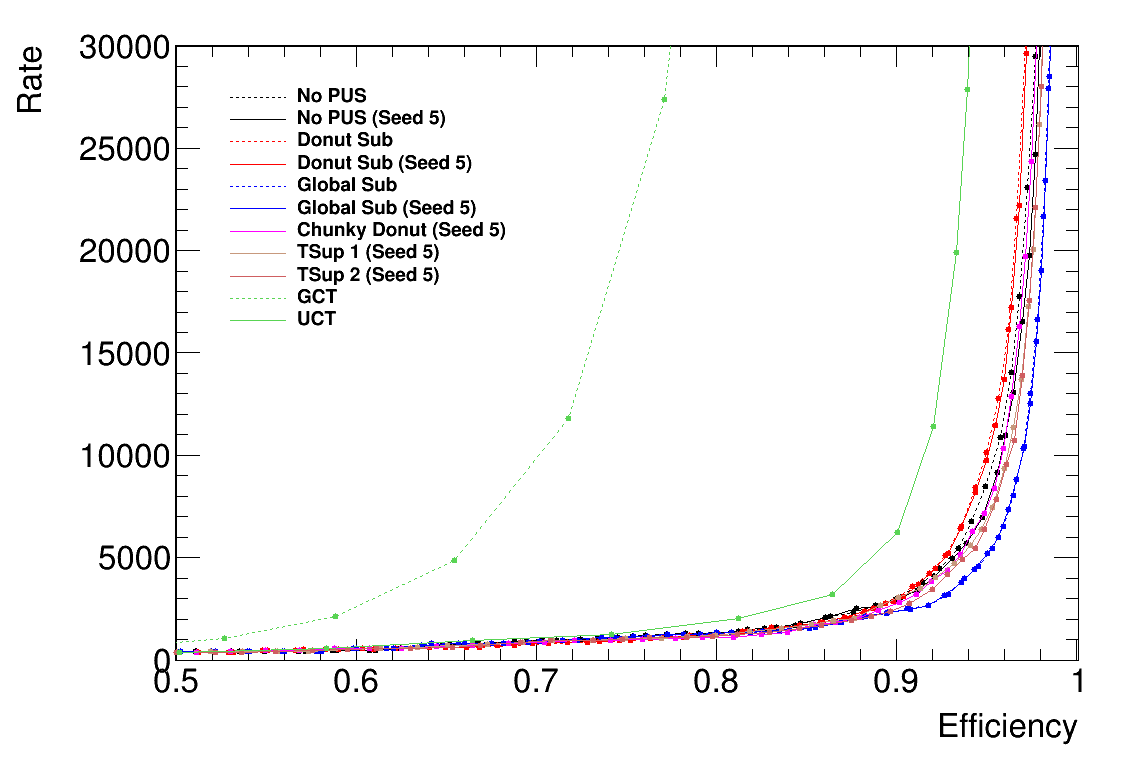
\includegraphics[width=0.52\textwidth]{figs/trigger/performance/quadJet_50}
    \label{fig:fourthJetRateEff}
  }
  \caption{ The normalised minimum bias rate (in Hz) against efficiency for a
  variety of thresholds of jet triggers
  made from jets with various \PUS schemes. Based on $t\bar{t}$ and
  minimum bias \MC simulation.}
  \label{fig:rateEffJet}
\end{figure}

\begin{figure}
  \centering
  \subfloat[$\HT>200~\gev$]{
    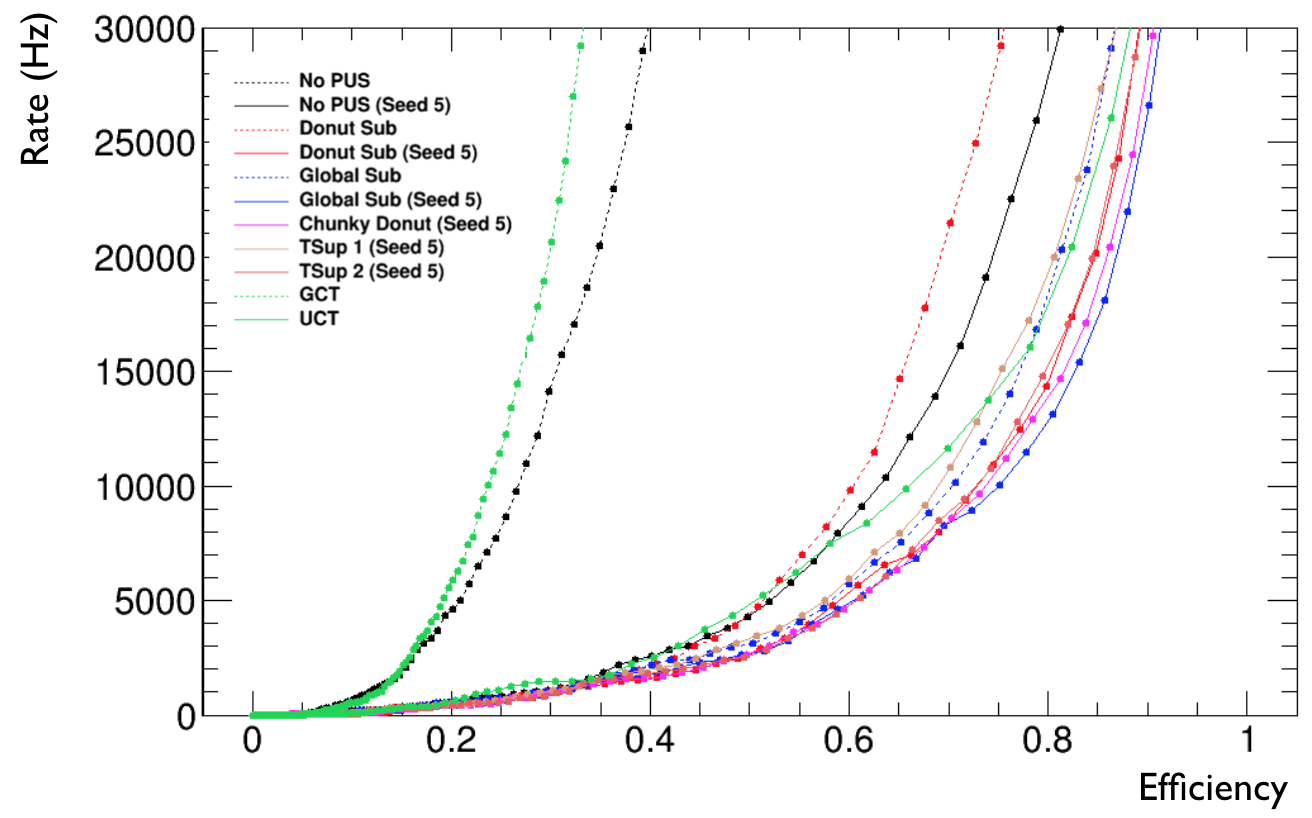
\includegraphics[width=0.5\textwidth]{figs/trigger/performance/ht_200}
    \label{fig:htRateEff}
  }~
  \subfloat[$\MHT>200~\gev$]{
    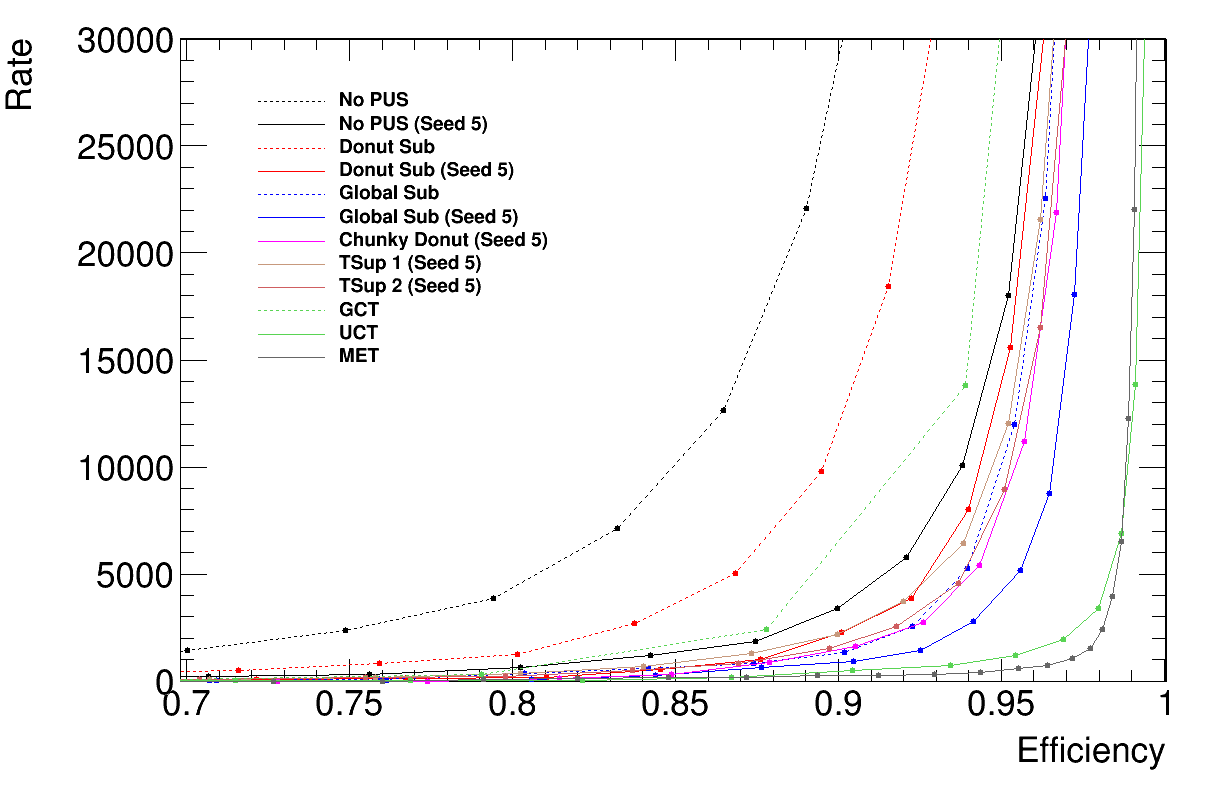
\includegraphics[width=0.5\textwidth]{figs/trigger/performance/mht_200}
    \label{fig:mhtRateEff}
  }
  \caption{ The normalised minimum bias rate (in Hz) against efficiency for a
  variety of thresholds of energy sum
  triggers made from jets with various \PUS schemes. Based on
  $t\bar{t}$ and minimum bias \MC simulation.}
  \label{fig:rateEffJet}
\end{figure}

\subsection{Conclusions}

After investigating the performance of the upgrade trigger algorithms
with simulation, it can be concluded that the upgrade algorithm
presents a significant improvement over the algorithm used in the \GCT
during Run~1 of the \LHC. The application of \PUS appears most useful
when summing jets to make trigger decisions. This is due to the fact
that \PU has the biggest effect on the energy of lower \pT jets from
the primary vertex and is most likely to produce low $\pT$ jets.
Overall, it can be inferred that the application of a seed threshold
effectively removes jets that originate from \PU. It is then possible
to successfully correct the energy of jets originating from the hard
scatter with both local and global \PUS methods. The chunky donut
algorithm performs most effectively for local \PUS. The $\rho$-area
form of \PUS seems to perform slightly better, but comes with
significant latency penalties when implemented in hardware. This is
particularly true when $\rho$-area \PUS is applied with a seed, as two
jet collections must be made, those with a seed and those without for
the $\rho$ calculation. Local forms of \PUS are also more robust
against localised detector faults, which can lead to issues with the
trigger inputs. With these considerations, it is concluded that the
$9\times9$ \TT jets with a 2.5~\gev seed threshold and chunky donut
\PUS is the most promising candidate for an upgrade algorithm. 

\section{Firmware emulation and testing}
\label{sec:emu}

After choosing a promising jet finder algorithm, it must be implemented
within the firmware of the \FPGA boards that will be used within the
Level-1 trigger. To provide a reference for validation of the
algorithm in firmware, a version is implemented in software, known as
the \emph{emulator}. The software is written to behave in a way that
is very close to the implementation in the \FPGA hardware. This
emulator is then included in the collaboration wide \emph{\CMS
software} and can be used to process data and simulation to produce an
emulated Level-1 trigger output. This is particularly useful when
testing the Level-1 trigger in simulation, for example when measuring
trigger efficiencies for a particular physics analysis. It is also
used to check that the Level-1 hardware is performing as expected
during the online data collection.

In the early stages of the firmware implementation, the jet finding
was validated against the algorithm in the emulator. A collection of
simulated events were processed by both the firmware within an \FPGA
and the emulator. After checking several of the jets were correctly
reconstructed by hand, the output of the firmware and emulator were
compared. As is shown in Fig.~\ref{fig:firmwareEmu}, the emulator and
firmware implementations both find jets in exactly the same positions
in the detector. These plots have a limited number of jets but demonstrate a first step towards a more
comprehensive validation of the emulator. This kind of testing was
extensively used to check the behaviour of the algorithm in the
firmware and to ensure the trigger decisions were properly emulated
in simulation.

\begin{figure}
  \centering
  \subfloat[]{
    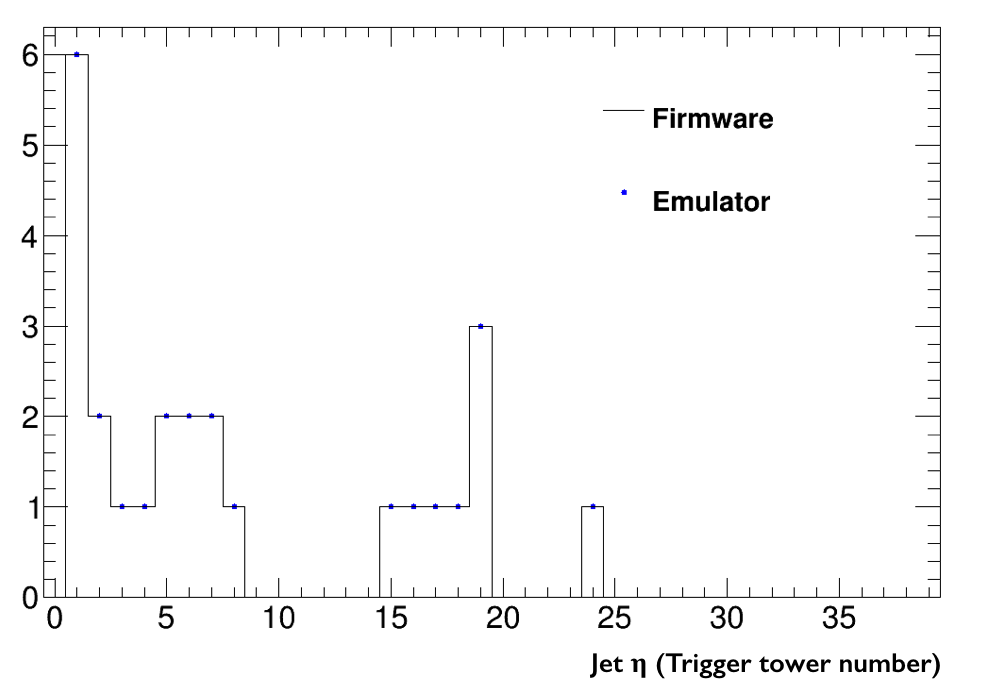
\includegraphics[width=0.48\textwidth]{figs/trigger/jetEtaEmulator}
    \label{fig:jetEtaEmulator}
  }~ 
  \subfloat[]{
    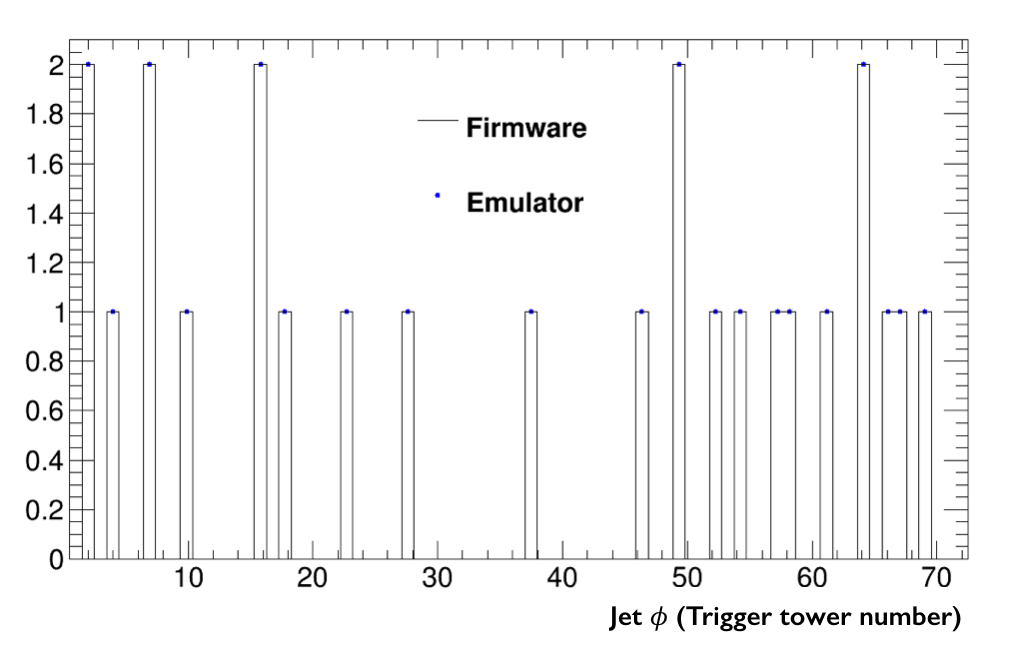
\includegraphics[width=0.52\textwidth]{figs/trigger/jetPhiEmulator}
    \label{fig:jetPhiEmulator}
  }
  \caption{Demonstration of agreement between the trigger algorithm
  implemented in firmware and emulated in software for simulation
  studies}
  \label{fig:firmwareEmu}
\end{figure}

The chunky donut $9\times9$ \TT jet finder algorithm has been fully
implemented into the upgrade hardware and successfully tested. It was
commissioned throughout the data collection during 2015 and has been
used to make the Level-1 trigger decisions when collecting data during
Run~2 from 2016 onwards.

%%% EXTRA PERFORMANCE STUFF FROM 9 MNTH THAT ISNT RELEVANT:

% The other purpose of PUS is to correct the energy of L1 jets
% contaminated with PU. The resolution of the jets as compared to Gen is
% defined as $\frac{p_T^{L1}-p_T^{Gen}}{p_T^{Gen}}$, being zero for
% perfect agreement. The PUS should act to remove the dependence of the
% resolution on the number of interactions in an event. In
% Figure~\ref{fig:resolution} it can be seen that the donut and global
% $\rho$ subtraction do flatten out the resolution for a representative
% bin of $p_T$ and $\eta$, whereas the seed on its own does not. 
% \begin{figure}
% 	\begin{center}
% 		\includegraphics[width=0.6\linewidth]{performance/pt_20to40_eta_-28to-14}
% 	\end{center}
% 	\caption{The resolution of L1 jets with $20<p_T<40$~GeV and with $-3<\eta<-1.2$ as a function of the number of interactions (NVTX)}
% 	\label{fig:resolution}
% \end{figure}
%correcting hard jets- response

% As a final performance test, the $H_T$ and $\cancel{H}_T$ as defined
% in Section~\ref{sec:alphaT} are plotted. If the PUS is too aggressive
% the $H_T$ will be too low when compared to Gen, or too high if it
% under subtracts. Figure~\ref{fig:htmht} shows that jets with a seed
% threshold most closely reproduce the $H_T$. Overall the PUS methods
% are under subtracting, however. The PUS does not improve the
% $\cancel{H}_T$ distribution, this is expected in the case that PU is
% distributed evenly.
% % \begin{figure}
% % 	\begin{center}
% % 		\includegraphics[width=0.5\linewidth]{performance/ht_ttbar}\put(-42,203){(a)}
% % 		\includegraphics[width=0.5\linewidth]{performance/mht_ttbar}\put(-42,203){(b)}
% % 	\end{center}
% % 	\caption{(a) The distribution of the total energy of jets in each event ($H_T$). (b) The distribution of the missing momentum of jets in an event ($\cancel{H}_T$).}
% % 	\label{fig:htmht}
% % \end{figure}
% %not killing important jets- ht mht

  % \chapter{Analysis strategy and event selection} %day1
\label{chap:selection}

Given the theoretical motivation for \BSM physics presented in
Chapter~\ref{chap:theory}, the next Chapters of this thesis describe a
search for \SUSY with the \CMS detector in $13~\tev$ proton collisions
produced by the \LHC. The analysis is designed to target \SUSY
produced through a strong force $pp$-interaction that decays hadronically via
\SM particles to a weakly interacting \LSP. The typical \SUSY models
considered in this search are those with gluino or squark pair
production. However, it is possible to generalise the search to look
for any \BSM signatures that have a weakly interacting particle with
significant momentum in the final state.
% introduce analysis and what the next chapters are about
% hadronic, inclusive, targets gluino and squark production but can be
% generalised to DM

As \SUSY has a significant number of free parameters, it can manifest
itself in a wide range of decay topologies. For this reason the
analysis is aimed to be as inclusive as possible, covering as much
parameter space as is feasible.  This is dictated by an ability to
predict the backgrounds from \SM processes with minimal uncertainties.
The search then attempts to find statistically significant excesses in
the data counts above those predicted for the various backgrounds. To
maximise the chance of seeing \BSM phenomena events are typically
required to have significant hadronic activity and missing momentum.  
% Robust strategy - minimise background uncertainties and look for
% excesses on top, in a conservative way (be very general here)


%%%%%%%%%%%%%%%%%%%%
\section{Challenges for a hadronic \BSM search}
\label{sec:challenge}

%main challenge in limiting and understanding backgrounds
The main challenge for a hadronic \BSM search is in limiting and
understanding the backgrounds, while maximising acceptance of a wide
range of potential \BSM signals. Within the analysis presented in this
Chapter the backgrounds are considered in two separate categories,
either as coming from a \QCD multijet process or from another \SM process
with neutrinos in the final state. As the search can look for generic
signatures that are indicative of \BSM processes, considerations of
signal modelling are not as important as constraining
and understanding these backgrounds.

\subsection{The QCD multijet background}
\label{sec:qcdMultijet}

The most abundant \SM process in $pp$-collisions at the \LHC is \QCD
multijet production through strong force interactions. This background
is orders of magnitude greater than other processes, as is evident
from the total \LHC cross section in Fig.~\ref{fig:xsecs}. The
majority of the \QCD background consists of events with multiple jets,
most commonly two, produced in a balanced configuration, with no
significant missing momentum, \MET or \MHT. A requirement on these
variables therefore significantly reduces the background. As
the abundance of such events is so large, however, mismeasurement of
the jets can lead to a significant \QCD background passing such
requirements. The fake missing energy can be introduced in a variety
of ways:
\begin{itemize}
\item{Detector effects leading to inefficiencies, such as jets
falling into regions of the detector that or uninstrumented or have a
reduced response due to hardware issues.}
\item{Fake additional energy being introduced. This can occur through
detector malfunctions, for example from problems in the readout
electronics. It can also be introduced through \PU that is attributed to
the primary vertex. Additionally, beam interactions that produce
particles outside the detector can introduce fake \MET signatures.}
\item{Issues at the reconstruction stage can also introduce fake \MET,
such as through under or over-corrections of jet energies, or through
the reconstruction algorithms missing physics objects that were
produced.}
\item{Through the measured energy of physics objects falling below
their selection threshold. }
\end{itemize}

Various techniques are applied to remove the background from these
effects, as described throughout this Chapter. Due to the nature of
these effects, which are often time dependent, they cannot be fully
accounted for in simulation. This fact, coupled with the difficulty in
accurately simulating \QCD processes due to uncertainties in the
theoretical calculations, makes constraining the multijet background a
significant challenge. 

It is also possible for the \QCD multijet background to be produced in
association with genuine \MET. This most often occurs in the case of
\emph{heavy flavour} \QCD, where a $b\bar{b}$ quark pair are produced
and at least one the $b$-quarks decay via the weak force, producing a
neutrino.  This is subdominant to the mismeasured multijet background,
but must still be accounted for. 
% heavy flavour qcd

% relevant to the trigger (cite back advantages from trigger chapter)

\subsection{Backgrounds from \SM processes with genuine
\MET}

The other class of \SM backgrounds are those produced with genuine
\MET. These processes only occur in the \SM through the electroweak
production of neutrinos. Due to the
mass scale of such electroweak processes, they commonly occur in
association with jets of significant momenta. The dominant
processes that constitute this background are \wj, \zj and \ttbar,
with residual backgrounds from other, lower cross section,
vector-boson or top production processes.

As a hadronic analysis does not look for leptons in the final state,
vetoing isolated leptons can help to reduce the background from the
\wj and \ttbar processes. In these cases a lepton is always produced
in association with the neutrino that results in the significant \MET.
Such events will only present a problem when the leptons are not
reconstructed, or do not appear to be isolated.  If the W boson
decays via a \tau-lepton that subsequently decays hadronically, the
event will not be removed by the lepton veto.  This is a comparably
small background, however.

The major irreducible background in \BSM searches with \MET comes from 
\znunu processes. They produce a pure missing energy signature with no
associated leptons to veto. Understanding this background to a high
degree of accuracy constitutes a significant challenge. However, due
to the better simulation of electroweak processes compared to \QCD
processes, the simulation can be used to help understand this
background with smaller uncertainties than the \QCD background.
% Z nu nu
%plots with backgrounds: http://www.hep.ph.ic.ac.uk/~mc3909/procs/

%%%%%%%%%%%%%%%%%%%%
\section{The \alphat analysis} 

The search for \SUSY described within this thesis revolves around
suppression of the \QCD multijet background to negligible levels
through the use of topological variables, including \alphat, described
in Sec.~\ref{sec:topoVars}. With negligible \QCD, the large
uncertainties that are usually prevalent when predicting this
background are greatly reduced. The use of these topological variables
also provides robustness against a wide range of mismeasurement
effects, which are particularly relevant when looking at early data,
when the issues present within the detector are not as well
understood. The remaining background from electroweak processes is
then estimated in a \emph{data-driven} way, minimising the
uncertainties from simulation.

During Run~1 of the \LHC, the \alphat analysis was performed
extensively to search for \SUSY. Datasets of $4.98~\ifb$ at
$\sqrt{s}=7~\tev$ and $18.5~\ifb$ at $\sqrt{s}=7~\tev$ have been
analysed, setting limits on \SUSY production within the context of
simplified models
\cite{Chatrchyan:2011zy,Khachatryan:2011tk,Chatrchyan:2012wa,Chatrchyan:2013mys,Khachatryan:2016pxa}.
The analysis presented within this thesis is performed on the data
collected during Run~2 of the \LHC at $\sqrt{s}=13~\tev$. The analysis
has been redesigned and optimised to perform well at the higher centre
of mass energy. Significant improvements have been made to improve the
sensitivity of the analysis and in characterising the various
backgrounds.

%%%%%%%%%%%%%%%%%%%%
\section{QCD multijet suppression with topological variables} %day2
\label{sec:topoVars}

As discussed in Sec.~\ref{sec:qcdMultijet}, a pure requirement on the
\MET of an event is not always enough to remove the \QCD multijet
background.  To effectively remove it, the mismeasurement that leads
to the fake \MET signature must be identified and used to remove
mismeasured events. This can be achieved by making use of topological
variables, which use specific facts about the topology of an event to
decide whether the \MET comes from mismeasurement or a weakly
interacting particle. 
%why topological variables work!! - fake met from detector cock ups

\subsection{The \alphat variable}
%introduce the variables and why they're useful

The dimensionless variable, \alphat, was originally proposed as the
$\alpha$ variable \cite{Randall:2008rw}, but changed to a transverse
quantity to make it more suitable for use in a hadron collider
\cite{CMS-PAS-SUS-08-005,CMS-PAS-SUS-09-001}. It is intrinsically
robust against jet energy mismeasurements in multijet systems. For a
dijet system, \alphat is defined as: 
\begin{equation}
\alpha_T=\frac{E_T^{j_2}}{M_T}, 
\end{equation} 
where $E_T^{j_2}$ is the transverse energy of the lower energy jet and
$M_T$ is the invariant mass of the dijet
system, defined as:
\begin{equation}
M_T=\sqrt{(\Sigma E_T^{j_i})^2-(\Sigma p_x^{j_i})^2-(\Sigma
p_y^{j_i})^2},
\end{equation}
where $E_T^{j_i}$ is the transverse energy of jet, $j_i$ and the $x$
and $y$ components of the transverse momentum are $p_x^{j_i}$ and
$p_y^{j_i}$ respectively.

In the case that the event in question is a perfectly measured dijet
event $E_T^{j_1}=E_T^{j_2}$ and both jets are back-to-back in $\phi$.
This results in a value of $\alphat=0.5$ when the momentum of each jet
is large in comparison with its mass, as is usually the case in
\QCD multijet events. If the jets are still back-to-back but one of
them is mismeasured, this will result in a value of $\alphat<0.5$.
However, in the case that the two jets are recoiling from a genuine
source of \MET, they will not be back-to-back and generally $\alphat>0.5$.

For events with more than two jets, a \emph{pseudo-dijet} system is
formed by summing jets vectorially to combine them.  The system chosen
is one that minimises $|\Delta E_T|$, the difference between the $E_T$
of each pseudo-jet, where $E_T$ is the scalar sum of the transverse
energies of all the jets in each pseudo-jet. This form of clustering
is chosen as it forms the most balanced configuration, making the
pseudo dijet event appear as close to an event with no mismeasurement
as possible. It leads to a generalised form of $\alpha_T$: 
\begin{equation}
\alpha_T=\frac{\Sigma E_T^{j_i}-\Delta
E_T}{2\sqrt{(\Sigma E_T^{j_i})^2-\cancel{H}_T^2}}.
\end{equation} 
In the case that there is no missing energy, $\Delta
E_T=\MHT=0$ and $\alphat=0.5$. However, if the energy of the jets is
mismeasured, the value of $\Delta E_T$ will be very close to \MET,
resulting in $\alphat<0.5$. When the jets are recoiling from genuine
\MET, $\Delta E_T\sim 0$ and $\alphat>0.5$.
  
The efficacy of an $\alphat$ cut in removing the \QCD multijet
background is evident in Fig.~\ref{fig:alphaT}. By
choosing an appropriate cut above $0.5$ it is possible to reduce the
multijet background to a negligible level.

\begin{figure}
	\begin{center}
		\includegraphics[width=0.7\linewidth]{figs/analysis/eventSelection/CMS-PAS-SUS-16-016_Figure-aux_001}%alphaT1_bkgd}
	\end{center}
  \caption{The $\alpha_T$ distribution for events with $H_T>200$ GeV
  that pass the pre-selection criteria (Sec.~\ref{sec:preselection}) when
  $\alphat<0.55$ and the signal selection criteria
  (Sec.~\ref{sec:signalregion}) when
  $\alphat>0.55$. The green dotted line shows the expected multijet
  QCD background that can be removed with an appropriate cut on
  $\alpha_T$}
	\label{fig:alphaT}
\end{figure}

\subsection{The \bdphi variable}

To further suppress the \QCD multijet background after applying an
\alphat cut the biased-$\Delta\phi$, \bdphi, variable is introduced.
This is a variation on the $\Delta\phi$ variable, which is usually
defined as the minimum azimuthal angle between the \MET and any jet in
the event. When calculating \bdphi, each jet is compared to the
\MHT, but the \MHT is recalculated as if the jet were not present in
the event. This leads to the definition:
\begin{equation}
\bdphi = \mathrm{min}(\Delta\phi(\vec{p_T^{j_i}},\vec{\MHT^{j_i}})),
\end{equation}
considered over every jet, $j_i$, and where
$\vec{\MHT^{j_i}}=\vec{\MHT}+\vec{p_T^{j_i}}$. The removal of the
probe jet from the event adds robustness to over-measurement, as well
as under-measurement, of the jet energies.
% introduce and explain

The \bdphi variable acts to remove events in which the \MET is
collinear with the jets, a typical feature of mismeasurement. However,
it also helps to remove the heavy flavour \QCD multijet background,
where a $b\bar{b}$ pair is produced and decays leptonically, producing
neutrinos. These neutrinos are a genuine source of \MET that are
typically boosted along the jet direction. In these cases the \bdphi
helps to reject the \QCD background that may have passed an $\alphat$
cut. The \bdphi distribution for multijet events and the remaining \SM
backgrounds is shown in Fig.~\ref{fig:bdphi}. A requirement on \bdphi
above $\sim 0.5$ will significantly reduce any \QCD multijet background.
%bDPhi augments alphaT when considering mismeasurement in heavy
%flavour qcd stuff
% show the plot from Mark

\begin{figure}
	\begin{center}
		\includegraphics[width=0.7\linewidth]{figs/analysis/eventSelection/CMS-PAS-SUS-16-016_Figure-aux_002}%alphaT1_bkgd}
	\end{center}
  \caption{The \bdphi distribution for events with $H_T>800$ GeV that
  pass the pre-selection criteria (Sec.~\ref{sec:preselection}). The
  green dotted line shows the expected multijet QCD background that
  can be removed with an appropriate cut on \bdphi}
	\label{fig:bdphi}
\end{figure}

%put the stuff about bDPhi over dPhi as in the ICHEP note

% One other variable that is commonly used to perform a similar
% background rejection to \bdphi is the minimum angular separation
% between the missing energy and leading four jets,
% $\Delta\phi(j_{1234},\MHT)_{min}$.  
To further demonstrate the efficacy of the \bdphi variable,
Fig.~\ref{fig:bDPhi_nominal} shows a comparison of the abilities of
the \bdphi variable to control the \QCD multijet background with a
similar jet-\mht angular variable \dphimhtj, the minimum azimuthal
separation between the \mht-vector and the leading four jets. The
\bdphi variable exhibits a distribution that is more sharply peaked
for the \QCD multijet background at low values and faster falling than
\dphimhtj,  \dphimhtj for QCD conversely has a broader distribution
with a larger leakage for a comparable azimuthal selection. This
demonstrates the ability of \bdphi to provide a better control of the
\QCD background while retaining acceptance of events with genuine
\mht, in this case represented by the V+jets, \ttbar and other
residual SM backgrounds with genuine \met. 

\begin{figure}[!h]
 \centering
 \subfloat[\bdphi distribution.\label{fig:bDPhi_dist}]{
 \includegraphics[width=0.5\textwidth]{figs/analysis/eventSelection/biasedDPhi_all_800}
 }
 \subfloat[\dphimhtj distribution.\label{fig:DPhiMht_dist}]{
 \includegraphics[width=0.5\textwidth]{figs/analysis/eventSelection/minDeltaPhiMht_all_800}
 } \\
 \caption{\bdphi and \dphimhtj distributions of MC simulation of the
 dominant analysis backgrounds
 after analysis selections for \scalht $> 800$ \GeV. }
 \label{fig:bDPhi_nominal}
\end{figure}

This is further demonstrated in Fig.~\ref{fig:bDPhi_roc}, where the
efficiency of retaining processes with genuine \mht is plotted against
the background efficiency for a series of \bdphi, \dphimhtj and
\dphimhtjall cuts, where \dphimhtjall considers all jets rather than
just the leading four. The points with a cut of $0.5$ are highlighted
as stars on the plot. As the general analysis strategy involves reducing
the \QCD multijet background to a negligible level while maximising
signal acceptance, these plots demonstrate that this is most
achievable with a cut on \bdphi. For the same threshold requirement of
$0.5$ on each variable, the \bdphi variable provides an efficiency for
multijet events that is approximately three orders of magnitude lower
than for \dphimhtj at the cost of approximately a factor $3$ reduction
in signal efficiency. The threshold on \bdphi required to give an
approximately equivalent suppression of QCD achieved with the
\dphimhtj variable is larger than 1.5, at the cost of a loss of a
factor $5$ in signal acceptance w.r.t. \bdphi. This also holds true in
the extreme case of a high jet multiplicity signal model.
Additionally, despite performing similarly to \bdphi for separating
the non-multijet from multijet backgrounds, the \dphimhtjall variable
performs worse for a high jet multiplicity signal model than \bdphi.

\begin{figure}[!h]
 \centering
 \subfloat[Acceptance of SM backgrounds with genuine \met vs QCD
 acceptance]{
 \includegraphics[width=0.5\textwidth]{figs/analysis/eventSelection/rateEffEwkQCD}
 }~
 \subfloat[High jet multiplicity \SUSY model acceptance vs QCD acceptance]{
 \includegraphics[width=0.5\textwidth]{figs/analysis/eventSelection/rateEffSignalQCD}
 } \\
 \caption{\bdphi, \dphimhtj and \dphimhtjall efficiency for simulation of processes with genuine
 \met vs QCD multijet background efficiency. The stars correspond to
 efficiencies with a cut of $0.5$ on each variable. A generic case of
 non-multijet process efficiency is considered in (a). In (b) we
 consider an uncompressed \SUSY model where gluinos are produced and
 decay via four tops to a pair of \acp{LSP}. 
%  This is the case in which \bdphi is
%  expected to have the lowest efficiency due to the very high jet
%  multiplicity of the model.
 }
 \label{fig:bDPhi_roc}
\end{figure}

Additionally the \bdphi variable displays robustness in the presence
of severe event mismeasurement, which is not present in \dphimhtj. A
mismeasurement is simulated by artificially lowering the \pt of the
jet that minimises the azimuthal separation variable to 41~\gev. Due
to the removal of the probe jet from the computation of \bdphi, the
distribution of angular separation Fig.~\ref{fig:shifted_bDPhi_dist}
is remains unchanged under severe mismeasurement. The \dphimhtj
variable is sensitive to such mismeasurement as both \mht and the rank
of the leading four jets are affected, resulting in a broader
distribution with increased leakage
Fig.~\ref{fig:shifted_DPhiMht_dist}.

\begin{figure}[!h]
 \centering
 \subfloat[QCD \bdphi distribution with mismeasurement.\label{fig:shifted_bDPhi_dist}]{
 \includegraphics[width=0.5\textwidth]{figs/analysis/eventSelection/shiftedMinBDPhi_all_800}
 }
 \subfloat[QCD \dphimhtj distribution with mismeasurement.\label{fig:shifted_DPhiMht_dist}]{
 \includegraphics[width=0.5\textwidth]{figs/analysis/eventSelection/shiftedMinDeltaPhiMht_all_800}
 } \\
 \caption{\bdphi and \dphimhtj distributions of QCD multijet simulation
 after analysis selections for \scalht $> 800$ \GeV in the case of
 severe mismeasurement. The
 total number of events that pass a $\Delta\phi > 0.5$ selection of the
 respective quantity are indicated. }
 \label{fig:bDPhi_mismeasured}
\end{figure}

\subsection{The missing energy ratio \mhtmet}
\label{sec:mhtmet}

After requirements are made on the \alphat and \bdphi variables, the
majority of events with \MHT introduced from jet mismeasurement are
removed. However, this does not take account of events in which jets
fall below their reconstruction threshold, detailed for this analysis
in Sec.~\ref{sec:physobj}. If several jets fall just below threshold
they can fake a significant \MHT. There is a much lower threshold
on the particles that go into the \MET calculation than the jets that
go into the \MHT threshold. Therefore, a requirement on the ratio of
these two variables helps to remove the background from mismeasurement
that falls below threshold. The extent to which this can remove the
remaining \QCD multijet backgroudn after the \alphat and \bdphi cuts
is shown in Fig.~\ref{fig:mhtDivMet}.
% removes soft stuff! given jet threshold

\begin{figure}
	\begin{center}
		\includegraphics[width=0.5\linewidth]{figs/analysis/eventSelection/mht40_pt_Div_metNoX_pt_all_all_80X_noOverflow_scaled0p6}%alphaT1_bkgd}
	\end{center}
  \caption{The \mhtmet distribution for \MC simulation with
  2.3~\ifb of $\sqrt{s}=13~\tev$ data overlaid. The
  normalisation of the \MC simulation is scaled so the data and \MC
  match.}
	\label{fig:mhtDivMet}
\end{figure}

%%%%%%%%%%%%%%%%%%%%
\section{Physics objects} %day3
\label{sec:physobj}

The analysis makes use of physics objects that are reconstructed with
the algorithms described in Chapter~\ref{chap:reconstruction}. As
there are many different input parameters within each of the
algorithms, the specific details relevant to the analysis are
described in this section. Jets are reconstructed to characterise the
hadronic activity within the event. Muons, electrons and photons are
reconstructed for a signal region veto and for selecting the \emph{control
regions} that are used for background estimation, detailed in
Sec.~\ref{sec:controlregions}. \emph{Isolated tracks} are additionally
reconstructed to provide an extra type of lepton veto when the leptons
are not fully reconstructed.

\subsection{Jets}
\label{sec:evSel_jets}

Jets are defined as sets of \PF candidates clustered by
the anti-$k_{T}$ jet clustering algorithm with
a distance parameter of 0.4. Additionally, \ac{CHS} is applied, charged
hadrons that can be traced back to \PU vertices are not clustered. The
four-vectors of the jets are then corrected with the procedure
outlined in Sec.~\ref{sec:reco_jec}.

The \emph{loose} working point jet quality criteria is chosen, defined
by the selections listed in Tab.~\ref{tab:loose-jet-id}. All jets are
required to contain at least part of their energy within the \ECAL and
\HCAL and must consist of at least one of each different type of
particle. This is effective at removing fake jets that are the result
of detector noise.  
%maybe show plots here?

Jets are also $b$-tagged with the \emph{medium} working point of the
algorithm described in Sec.~\ref{sec:reco_btag}. This is obtained with
a cut of $>$ 0.800 on the algorithm discriminator variable. This
results in a gluon/light-quark mis-tag rate of $\sim$1 \% (where
\emph{light} means $u$, $d$ and $s$ quarks), a charm-quark mis-tag
rate of $\sim$10 \% and a b-quark b-tag efficiency of about 60 \%. 

\begin{table}[ht!]
  \caption{The \emph{loose} jet ID requirements. \label{tab:loose-jet-id}}
  \centering
  \begin{tabular}{ ccc }
    \hline
    \hline
    Variable & cut & notes \\ \hline
    \multicolumn{3}{c}{$-3.0 < \eta_{\mathrm{jet}} < 3.0$} \\ \hline    
    Neutral Hadron Fraction & $<0.99$ & - \\
    Neutral Electromagnetic Fraction & $<0.99$ & - \\
    Number of constituents & $>1$ & - \\
    Charged Hadron Fraction & $>0$ & only for $|\eta_{\mathrm{jet}}| < 2.4$ \\
    Charged Multiplicity & $>0$ & only for $|\eta_{\mathrm{jet}}| < 2.4$ \\
    Charged Electromagnetic Fraction & $<0.99$ & only for $|\eta_{\mathrm{jet}}| < 2.4$ \\ \hline
    \multicolumn{3}{c}{$|\eta_{\mathrm{jet}}| > 3.0$} \\ \hline        
    Neutral Electromagnetic Fraction & $<0.90$ & - \\
    Number of Neutral Particles & $>10$ & - \\
    \hline
    \hline
  \end{tabular}
\end{table}

\subsection{Muons}
\label{sec:muon-id}
Two types of selection are made on muons depending on whether they are
used to carry out the veto in the signal region or used for selecting
one of the control regions. A tighter criteria is used for the control
region, muons are required to be well isolated and be
reconstructed with the global algorithm, as detailed in
Sec.~\ref{sec:muons_reco}. The muon must consist of a track
with at least 5 inner layer hits, a good fit $\chi^2$, good compatibility with
the primary vertex and significant muon chamber hits. The isolation in
the control region uses the relative isolation algorithm
defined in Sec.~\ref{sec:reco_iso} with effective-area
correction, it is required that $I^{\textrm{rel}}<0.15$.  

For the purpose of vetoing muons in the signal region, a looser
working point is used, which provides $\sim98\%$ efficiency. The
muon is just required to be classified within the \PF algorithm and
reconstructed with the global or tracker muon
algorithms. The
mini-isolation algorithm is utilised with effective-area \PU
correction $I^{\textrm{rel}}_{\textrm{mini}} < 0.2$. The reconstructed
muon must have a $\pT>10~\gev$ and be within $|\eta|<2.1$.

\subsection{Photons}
\label{sec:photon-id}

Photons are identified according to a \emph{tight} working point
definition ($\sim$ 71 $\%$ efficiency) and required to be well
isolated.  A \PF-based isolation which considers neutral and charged
hadrons separately is used with a cone size $\Delta R<0.3$
and effective-area corrections are applied to remove the
effects of pileup.  Table \ref{tab:photon-id-gamma}
summarises the isolation selection used. There are additional
requirements on the ratio of \HCAL and \ECAL deposits and the
kinematics of the deposits within the \ECAL. The reconstructed
photon must have a $\pT>25~\gev$ and be within $|\eta|<2.5$.

\begin{table}[ht!]
  \caption{Photon isolation criteria (\emph{tight} working point). The
  energy of particles within the isolation cone must be less than the
  value in the column.\label{tab:photon-id-gamma}}
  \centering
  \footnotesize
  \begin{tabular}{ ccc }
    \hline
    \hline
    Categories                    & Barrel                             & EndCap                             \\
    \hline
    PF charged hadron isolation   & 1.66 GeV & 1.04 GeV                          \\
    PF neutral hadron isolation   & 0.14 + $ e^{0.0028 \times \pt^{\gamma} + 0.5408}$  &  3.89 + 0.0172 $\times$ $\pt^{\gamma}$\\
    PF photon isolation           & 1.40 + 0.0014 $\times$ $\pt^{\gamma}$ & 1.40 + 0.0091 $\times$ $\pt^{\gamma}$ \\
    \hline
    \hline
  \end{tabular}
  \end{table}

\subsection{Electrons}
\label{sec:electron-id}

In order to veto electrons a \emph{loose} working point definition
($\sim$ 90 $\%$ efficiency) is used. There are requirements on the
ratio of \HCAL and \ECAL deposits, criteria to remove photons that
have converted within the tracker, a minimum number of tracks required
and kinematic requirements on the deposit within the \ECAL. Electrons
are also require required to be isolated with the effective-area
corrected mini-isolation algorithm.  Isolated electrons are defined by
$I^{\textrm{rel}}_{\textrm{mini}} < 0.1$. The reconstructed electron
must have a $\pT>10~\gev$ and be within $|\eta|<2.5$.

% Table \ref{tab:ele-id} summarises the identification 
% selection used. 
%
% \begin{table}[h!]
%   \caption{Electron identification (``tight'' working point).\label{tab:ele-id}}
%   \centering
%   \footnotesize
%   \begin{tabular}{ lcc }
%     \hline
%     \hline
%     Categories                                               & Barrel    & EndCap    \\
%     \hline
%     $\Delta \eta_{In}$                                       & 0.0105   & 0.00814  \\
%     $\Delta \phi_{In}$                                       & 0.115    & 0.182  \\
%     $\sigma_{i\eta i\eta}$                                   & 0.0103    & 0.0301  \\
%     H/E                                                      & 0.104    & 0.0897   \\
%     d0 (vtx)                                                 & 0.0261    & 0.118  \\
%     dZ (vtx)                                                 & 0.041    & 0.822  \\
%     $\lvert(1/E_{\textrm{ECAL}} - 1/p_{\textrm{trk}})\rvert$ & 0.102     & 0.126  \\
%     Missing hits (inner tracker)                             & 2         & 1         \\
%     Conversion veto                                          & yes       & yes   \\
%     \hline
%     \hline
%   \end{tabular}
%   \end{table}


\subsection{Isolated tracks}
\label{sec:SIT}

A single isolated track comprises a charged PF candidate with $\Pt >
10 \gev$, $\Delta z(\mathrm{track}, \mathrm{\ac{PV}}) < 0.05 \,
\mathrm{cm}$ and with a relative isolation smaller than 0.1, where the
isolation is determined from the sum of the \Pt of the charged PF
candidates within $\Delta R < 0.3$. It is useful for identifying W
bosons through their leptonic decays, when the lepton is not fully
reconstructed: W $\rightarrow$ $\mu \nu$, W $\rightarrow$ $e\nu$, and
W $\rightarrow$ $\tau$($\rightarrow l$) $\nu$.  Single prong decays of
the tau lepton can also be identified: W $\rightarrow$ $\tau$
($\rightarrow$ h$^{\pm}$ + n$\pi^{0}$) $\nu$. 
%Events in the signal region and all control regions (ignoring the
%selected muons) containing a SIT candidate identified with these
%criteria are vetoed.

\subsection{Energy sums}

Missing transverse momentum (\MET) is reconstructed as described in
Sec.~\ref{sec:met_reco} and the the Type-I \MET energy correction is applied.
The \met is used in the definition of 
the transverse mass, $M_{T}$, which is in turn used as part of
the selection criteria that define the single muon control sample 
(Sec.~\ref{sec:controlregions}), and for the $\mhtmet$ cleaning
filter, described in Sec.~\ref{sec:mhtmet}.

The \HT and \MHT energy sums are constructed with the jets outlined in
Sec.~\ref{sec:evSel_jets}, which are subject to the kinematic requirements of
$\pT>40$~\gev and $|\eta|<3$.

%%%%%%%%%%%%%%%%%%%%
\section{Trigger strategy}
\label{sec:trigStrat}

As \SUSY models have a lot of freedom in how they are manifest, a
guiding principle of the analysis is to maintain acceptance of as much
phase space as possible. Despite some \SUSY models being ruled out at
energies $O(100~\gev)$, models with compressed spectra are still poorly
constrained in this regime. The trigger strategy therefore revolves
around maintaining as low an energy threshold as possible given the
very high rate of \QCD multijet processes. To select for events with
significant hadronic activity and missing energy, triggers are used
that rely on the \HT and \MHT of the events. Additionally, including
topological variables, such as \alphat, in the \HLT allow events to be
collected with $\HT$ as low as $200~\gev$.

To collect events that are of general use to hadronic analyses, the
$\HT$ of each event is reconstructed within the \HLT. This is carried
out with a custom form of \PF, that is designed to work in a way that
is quick enough given the time the trigger has to make a decision. To
further help with this timing constraint, the \HT is calculated with
jets clustered from only calorimeter deposits and a looser constraint
is made, reducing the load on the \PF reconstruction. This allows for
all events that pass $\HT>800~\gev$, calculated by the \HLT,
to be collected. When carrying out full online reconstruction, this
results in a $\sim 100\%$ efficiency for events with an offline
$\HT>900~\gev$. 

To be able to efficiently collect events with lower
values of \HT, the \alphat variable is calculated within the \HLT. A
requirement is made on both \alphat and \HT for a series of different
\HT thresholds. These requirements are chosen to limit the rate of the
\alphat-\HT triggers to an acceptable level, while maintaining low
acceptance of events with low \HT. 

There are also general purpose missing energy triggers that require
both an \MHT and \MET threshold to be surpassed within the \HLT.
Including events selected by these triggers helps to increase the
efficiency across the phase space. These variables, however, are quite sensitive to
running conditions and mismeasurement, so are not as robust against
the \HLT rate as the \alphat-\HT triggers. The full list of
triggers used to collect data for the signal region of the \alphat
analysis can be seen in Tab.~\ref{tab:triggers}.

The events in the control regions are collected with muon or photon
triggers, where the \HLT requires at least one of these objects above
a certain energy threshold. Due to the lower rate of events
containing leptons, these triggers are at full efficiency for their
requirements in the analysis. The specific triggers used are also listed in
Tab.~\ref{tab:triggers}.

\begin{table}[h!]
\caption{Trigger thresholds of the Level-1 and \HLT paths for the
hadronic signal region and the leptonic control regions. {\bf FIXME} check the CR l1 thresholds }
\footnotesize
\centering
\begin{tabular}{c|c|c} 
Analysis region   & Level-1 requirements & \HLT requirements                                                \\
\hline
 & $\HT>240~\gev~\textrm{or}~\MET>70~\gev$ & $\HT>200~\gev,~\alphat>0.57,\MET>90~\gev$ \\
 & $\HT>240~\gev~\textrm{or}~\MET>70~\gev$ & $\HT>250~\gev,~\alphat>0.55,\MET>90~\gev$ \\
 & $\HT>240~\gev~\textrm{or}~\MET>70~\gev$ & $\HT>300~\gev,~\alphat>0.53,\MET>90~\gev$ \\
Signal & $\HT>240~\gev~\textrm{or}~\MET>70~\gev$ & $\HT>350~\gev,~\alphat>0.52,\MET>90~\gev$ \\
 & $\HT>240~\gev~\textrm{or}~\MET>70~\gev$ & $\HT>400~\gev,~\alphat>0.51,\MET>90~\gev$ \\
 & $\HT>240~\gev$ & $\HT>800~\gev$ \\
 & $\MET>70~\gev$ & $\MET>90~\gev~\textrm{or}~\MHT>90~\gev$ \\
\hline
\mj& $\pT^{\mu}>10~\gev$ & $\pT^{\mu}>22~\gev$ \\
\mmj& $\pT^{\mu}>10~\gev$ & $\pT^{\mu}>22~\gev$ \\
\gj& $\HT>240~\gev~\textrm{or}~\pT^{\gamma}>25~\gev$ & $\HT>800~\gev~\textrm{or}~\pT^{\gamma}>175~\gev$ \\

\end{tabular}
\label{tab:triggers}
\end{table}

%%%%%%%%%%%%%%%%%%%%
\section{Pre-selection}%day4
\label{sec:preselection}

To ensure that all events considered by the analysis have
significant hadronic activity and missing energy, a pre-selection is
carried out on all events considered in the signal and control
regions. It is described within this section.

Events are required to contain at least one $p_T>100$~GeV jet,
with all other jets being considered if they have $p_T>40$~GeV and are
well reconstructed in the central region, $|\eta|<3$. If any jets
fall outside the $\eta$ range, the event is vetoed. This ensures there
is no significant energy deposited within the region of the detector
with no tracker. As most \BSM physics scenarios result in the
production of particles at a high mass scale, they are expected to deposit
most of their energy centrally. Therefore, this \emph{forward jet
veto} does not significantly effect the signal efficiency for most
models. The \QCD multijet background consists of many
soft scattering events, which typically deposit a significant
proportion of energy within the forward region. As this is the case,
the forward jet veto also helps to reduce the multijet
background.

Significant hadronic activity is selected by requiring $H_T>130$~GeV.
This cut is primarily motivated by the trigger threshold, it is the
lowest \HT value that can be reached with a reasonable trigger rate
and efficiency. To ensure there is significant missing energy, it is
required that $\MHT>200~\gev$.  This threshold is chosen as roughly
equivalent to the magnitude of the \MHT requirement made by the
\alphat cuts on dijet events within the signal region when there is no
significant mismeasurement. 
%could expand on this with formula?

Additionally, to remove events with significant energy deposits that
have not been reconstructed as jets, a requirement is made on the
ratio $\mhtmet<1.25$, as motivated in Sec.~\ref{sec:mhtmet}.  When
this requirement is made for the control regions, the \MET is
reconstructed ignoring the leptons or photons that define the
particular region. This ensures a fair comparison with \MHT and allows
the lepton to simulate the missing momentum in the 
signal region.

To ensure that beam conditions or reconstruction effects have
not produced a spurious \MET, extra filters are applied. The filters
used are designed to remove instances of fake \MET while retaining
a high efficiency for real physics events, they are described in the
following \cite{1748-0221-10-02-P02006}.
\begin{itemize}
\item{The primary vertex must be well reconstructed, within
$|z|<=24$~cm of the proton collision region and $d_{xy}<2$~cm from the
beam line}
\item{Beam interactions exterior to the detector, \emph{beam halo} effects,
are removed by vetoing events with \ac{CSC} and calorimeter energy
deposits consistent with interactions from particles outside the
detector}
\item{Noise, caused by particle interactions with the read-out system
and dead regions within the \HCAL, are removed with the \emph{HBHE
noise and isolation filters}}
\item{Anomalous signals within the \ECAL endcap supercrystals are removed
with the \emph{\ECAL Endcap SC Noise filter} and \emph{\ECAL \ac{TP}
filter}}
\item{Events with misidentified straight tracks that are reconstructed
to have a large \pT are removed by the \emph{bad track filter}}
\end{itemize}

Finally, two additional vetoes are applied to ensure events are purely
hadronic with minimal misreconstruction. Any events that contain a
\ac{SIT} with $\pT > 10\gev$ and within $|\eta| < 2.5$ is vetoed. This
reduces the background from single pronged $\tau$ decays and
misreconstructed leptons. Within the muon control regions this track
is ignored if it is within $\Delta R <0.02$ of an identified lepton.
Additionally, any events with jets that do not pass the loose
requirements described in Sec.~\ref{sec:evSel_jets} are vetoed.

A summary of the pre-selection requirements is shown in
Tab.~\ref{tab:preselection}.

\begin{table}[h!]
  \caption{Summary of the pre-selection criteria.}
  \centering
  \footnotesize
  \begin{tabular}{ ll }
    \hline
    Selection                     & Requirement                     \\
    \hline
    ``MET filters''               & \parbox[t]{10cm}{Primary Vertex, CSC Beam Halo,
      HBHE Noise and Isolation, \\ ECAL Endcap SC Noise, ECAL TP, bad
      track filter}         \\
    Jet acceptance                & $\pT > 40\gev$, $|\eta| < 2.4$                      \\
    Lead jet acceptance           & $\pT > 100\gev$, $|\eta| < 2.4$                   \\
    Forward jet veto              & $\pT > 40\gev$, $|\eta| > 2.4$                     \\
    \HT requirement               & $\HT > 200\gev$                  \\
    \mht requirement              & $>200\gev$         \\  
    \mhtmet requirement              & $<1.25$         \\  
    Single isolated track veto      & $\pT > 10\gev$, $|\eta| < 2.5$    \\  
    \hline
  \end{tabular}
  \label{tab:preselection}
\end{table}

\section{The signal region}
\label{sec:signalregion}

The signal region selection is chosen to be as inclusive to potential
\BSM signatures in the jets and missing momentum final state, while
minimising the effects of mismeasurement and contributions from \SM
processes with genuine \MET. To reduce the background from decays via
W bosons, a veto is made on any leptons that are identified as
described in Sec.~\ref{sec:physobj}. To maintain a fully hadronic
final state any events containing reconstructed photons are also
vetoed.

After the pre-selection requirements, there is still a significant
multijet background in the signal region. This is reduced to a
negligible level with a \HT dependent cut on the \alphat of the event.
Along with this, a cut is made on the \bdphi variable to ensure any
multijet background that passes the \alphat cut is removed. A summary
of these cuts can be seen in Tab.~\ref{tab:atCut}. The \alphat cuts
are loosened as a function of \HT in correspondence with the trigger
thresholds. At lower values of \HT the high trigger rate requires
a higher \alphat threshold, due to the fact that the multijet
background falls off as a function of \HT. In the case that events
have just one identified jet, the value of \alphat is undefined. In
these \emph{monojet} events there is no \alphat cut. The \bdphi
variable is also undefined with 40~\gev jets. To get around this issue
and provide multijet discrimination in monojet events, the \pT
threshold on jets used to calculate the \bdphi variable is reduced to
25~\gev. In the case that there are no other jets between 25 and
40~\gev the event is allowed into the signal region.

It is observed that the beam halo \MET filter, described in
Sec.~\ref{sec:preselection}, is ineffective in removing all cases of
mismeasurement from the signal region. A requirement that the \ac{CHF}
of the lead jet is above $10\%$ is enough to negate this effect. This
cut is demonstrated to in Fig.~\ref{fig:leadJetCleaning}. Due to the
fact that the proton beam is steered within the horizontal plane of
the \LHC, beam halo effects manifest themselves at \phi values of $0$
and $\pi$. The application of the \ac{CHF} cut removes the spikes in
the leading jet $\phi$ distribution at these values.

\begin{table}[h!]
  \centering
  \footnotesize
  \begin{tabular}{ l|ccccccccc }
    \hline
    \scalht (GeV)      & 200       & 250       & 300       & 350       & 400       & 500       & 600 &  $>$900    \\
    \hline                                                                                     
    \alphat threshold  & 0.65      & 0.60      & 0.55      & 0.53      & 0.52      & 0.52      & 0.52 & --    \\
    \hline
    \bdphi threshold  & 0.5      & 0.5      & 0.5      & 0.5      &
    0.5      & 0.5      & 0.5 & 0.5    \\
    \hline
  \end{tabular}
  \caption{The \alphat and \bdphi thresholds versus
    lower bound of \scalht bin. For all \HT bins satisfying $\HT >
    900\gev$, no \alphat cut is applied. No \alphat requirement is
    imposed in the case that there is only one reconstructed jet.}
  \label{tab:atCut}
\end{table}

% \begin{figure}[h!]
%   \centering
%     %{\includegraphics[width=0.32\textwidth]{figures/selection/jet_chHEF_mono_all_before.pdf}}
%     {\includegraphics[width=0.32\textwidth]{figures/selection/jet_phi[0]_mono_all_before.pdf}}
%     {\includegraphics[width=0.32\textwidth]{figures/selection/jet_phi[0]_mono_all_after.pdf}}
%     \caption{Distributions in the signal region of the jet charged hadron
%     energy fraction (CHF) (Left), jet $\phi$ direction (Centre), and jet $\phi$
%     direction after applying a requirement of {CHF~$>0.1$}. The large excess in data
%     at charged hadron fractions close to zero and ${\phi = 0, \pi}$ is consistent with beam
%     halo effects, and is effectively suppressed by the aforementioned selection.}
%     \label{fig:leadJetCleaning}
% \end{figure}
\begin{figure}[!h]
 \centering
 \subfloat[No \ac{CHF} cut]{
 \includegraphics[width=0.5\textwidth]{figs/analysis/eventSelection/jet_phi[0]_mono_all_before}
 }
 \subfloat[Lead jet \ac{CHF}>0.1]{
 \includegraphics[width=0.5\textwidth]{figs/analysis/eventSelection/jet_phi[0]_mono_all_after}
 } \\
  \caption{Distributions in the signal region of the jet $\phi$
  direction (a), and jet $\phi$ direction after applying a requirement
  of \ac{CHF}~$>0.1$. The large excess in data at charged hadron
  fractions close to zero and ${\phi = 0, \pi}$ is consistent with
  beam halo effects, and is effectively suppressed by the
  aforementioned selection.}
  \label{fig:leadJetCleaning}
\end{figure}

\section{The control regions}
\label{sec:controlregions}

To carry out a data-driven estimation of the \SM backgrounds, several
control regions are defined. They are chosen to be orthogonal to the
signal region by inverting at least one of the requirements. To estimate
processes with genuine \MET, control regions are populated with events
that contain at least one muon or photon. The muons or photons are then
ignored when calculating any of the event level variables, such as
\alphat or \bdphi, to simulate the signature left by neutrinos or
cases in which the lepton is not properly reconstructed. Extrapolation
from these control regions with guidance from simulation is then used
to estimate the background counts in the signal region, as described
in Chapter~\ref{chap:backgroundPred}. The pre-selection criteria
is applied to each control region and ensures they are in a similar
phase-space to the signal region. As the requirement of an isolated
lepton or photon already selects electroweak processes and rejects
\QCD multijet processes there is no need for an \alphat or \bdphi
requirement in these control regions. Removing these requirements
significantly increases the number of events available within each
control region. This reduces statistical uncertainties when they are
used for background estimation.

\subsection{The \mj control region}

The selection criteria for the \mj control region are chosen to select
events containing W bosons that are produced in association with
jets and decay to a muon and a neutrino. Exactly one muon that passes
the control region selection criteria, described in Sec.~\ref{sec:muon-id}, with
$\pT>30~\gev$ and $|\eta|<2.1$ is required. The muon is required to be
separated from other jets by $\Delta R(\mu,\mathrm{jet})>0.5$. If any
other leptons or photons are present in the event then it is vetoed, as
in the signal region.

To help ensure events containing W bosons are selected a requirement
is also made on the transverse mass of the W candidate. It is
approximated by taking the transverse mass between the \MET and the
muon, and is then required to be compatible with the muon mass,
$30<M_T(\mu,\MET)<125~\gev$. This effectively suppresses any residual
\QCD multijet background that pass the muon requirement.
%plots??

\subsection{The \mmj control region}

The selection criteria for the \mmj control region are chosen to
select events containing Z bosons that are produced in association
with jets and decay to a pair of muons. They are selected to be
kinematically similar to the main irreducible background in the signal
region, \znunu. Exactly two muons are required that
pass tight selection criteria with $\pT>30~\gev$ and $|\eta|<2.1$.
They are also required to be separated from jets as in the \mj control
region. Again, if any other leptons or photons are present the event
is vetoed.

To maximise the selection of events containing Z bosons the
invariant mass of the two muons is required to be compatible with the
Z mass, $m_Z$. Events are used if they are within a 25~\gev window,
$m_Z-25<M_{\mu_1\mu_2}<m_Z+25~\gev$.

\subsection{The \gj control region}

The \gj control region is defined to provide a sample of photon events
with significant hadronic energy. High energy photons have similar
kinematic properties to $Z$ bosons, which allows this control region
to augment the prediction of the \znunu background. To
ensure the mass of the Z boson has a negligible effect when making
this assumption, a single photon is required with $\pT>200~\gev$ and
$|\eta|<1.45$. This selection also maintains a high trigger
efficiency, the photon trigger rate is significantly greater than the
muon rate so has a higher \pT threshold. To ensure the photon did not
originate from a hadronic jet, events with $\Delta
R(\mathrm{jet},\gamma)<0.5$ are vetoed. Events containing any photons
or lepton other than the single selected photon are vetoed.

\subsection{The hadronic control regions}

While the above control regions are useful for estimating the \SM
backgrounds with genuine \MET, some hadronic control regions are
defined to quantify the residual \QCD multijet background that remains
in the signal region. To define these control regions, all the signal
region requirements are made except for the requirement on \bdphi or
\mhtmet being inverted. The use of these control regions is
discussed in Sec.~\ref{sec:qcdEstimation}.

\section{Event categorisation}
\label{sec:categorisation}

To help to separate signal from background for a wide range of
different signal hypotheses, events are a categorised based on the
number of jets, \nj, their total hadronic energy, \HT, the magnitude
of the missing hadronic energy, \MHT, and the number of jets tagged as
a $b$-quark, \nb. These particular variables are chosen because many
\BSM models predict excesses in the tails of the distributions that
are not predicted by the \SM. For example, many \SUSY models favour
decays via top quarks, resulting in a significant number of $b$-tagged
jets and high \nj multiplicities. All \BSM models targeted by this
search also produce significant \MHT.

Along with straightforward binning in the categorisation variables,
events are also split based on their jet topology. They are
categorised as either \emph{symmetric}, \emph{asymmetric} or
\emph{monojet} depending on the \pT of the second leading
jet. In the case that the second leading jet has $\pT>100~\gev$ the
event is defined as symmetric. This category of events targets the
typical \SUSY pair production scenarios when there is a significant
mass splitting between the \SUSY parent and the \LSP. However, in the
case that there is a compressed spectrum, a small mass splitting,
there is unlikely to be significant energy in the \SM decay products
of the \SUSY system. Sensitivity to these events can be gained by
selecting events with significant \ac{ISR} or \ac{FSR} that have
recoiled from the invisible \SUSY system. This topology is targeted by
the monojet and asymmetric jet category which require the second jet
to have $\pT<40~\gev$ or $40<\pT<100~\gev$ respectively.
%{\bf FIXME} add something that differentiates the different categories?

A summary of the event categorisation for the \nb, \njet and \HT
variables is shown in Tab.~\ref{tab:eventCategorisation}. This is
mirrored in the control and signal regions. The \MHT dimension is
treated slightly differently, with a variable binning based on \HT.
This will be discussed further in Sec.~\ref{sec:mhtDim}.

\begin{table}[h!]
  \caption{Summary of the \nj, \nb, \HT binning.}
  \label{tab:eventCategorisation}
  \centering
  \begin{tabular}{ cl }
    \hline
    Variable & Binning \\
    \hline
    \multirow{3}{*}{\njet}
     & Monojet:    $\njet=1$ \\
     & Asymmetric: $\njet \geq 2$ \\
     & Symmetric:  $\njet =2,3,4,5 \geq 6$ \\
    \hline
    \nb & $\nb=0,1,2,3,\geq 4$ \\
    \hline
    \scalht (GeV) & 200-400, 400-600, 600-900, 900-1200, $>$1200 \\
    \hline
  \end{tabular}
\end{table}

%%%%%%%%%%%%%%%%%%%%
%\section{Further optimisation of event selection}
% something about minChi here?

  % \chapter{Background prediction} %day 1
\label{chap:backgroundPred}

%%%%%%%%%%%%%%%%%%%%
\section{Dataset} %day 1
\label{sec:dataset}

The data used by this version of the analysis comprises $12.9~\ifb$ of
proton-proton collisions produced by the \LHC and recorded by \CMS
during the first few months of 2016. The data for this analysis are
collected with the triggers described in Sec.~\ref{sec:trigStrat}.

%%%%%%%%%%%%%%%%%%%%
\section{Simulated event samples} %day 1
\label{sec:simEvents}

A selection of simulated \MC samples are used to help estimate the \SM
backgrounds and possible signal within the analysis. The samples are
generated with the methods discussed in Sec.~\ref{sec:mc_reco}. The
majority of samples, including the signal model samples, are simulated
with \textsc{MadGraph5} \cite{Alwall:2011uj,Alwall:2014hca} at \LO
accuracy: \QCD multijet samples, Drell-Yan + jets, \wj, \zj and \gj.
Using the same generator at \NLO accuracy, the s-channel single top,
{\ttbar}W and {\ttbar}Z events are simulated. Additionally, the
\textsc{powheg} \cite{Alioli:2010xd,Re:2010bp} generator is used at
\NLO accuracy to describe the t-channel and tW-channel production of
single top quarks. Diboson (WW, WZ, ZZ) production is simulated using
\textsc{pythia} 8.2 \cite{Sjostrand:2014zea}. This generator is also
used to simulate the decays of the sparticles within the signal
models. The cross-sections used for total event yield normalisation
are calculated at \NLO and \NNLO precision
\cite{Alwall:2011uj,Re:2010bp,Alioli:2009je,Gavin:2010az,Melia:2011tj,Czakon:2011xx,Gavin:2012sy}.
The detector response is simulated using \textsc{Geant4}
\cite{Agostinelli:2002hh}.

As the simulations cannot fully recreate all the effects within data a
series of corrections are made on the event yields predicted by the
simulation. They are described in the rest of this section.

\subsection{Pileup reweighting}

When the \MC samples are generated the number of \PU collisions are
simulated as Poisson distributed about a chosen rate that is expected
to be close to that obtained in data. As the simulation is produced
before the data is collected and the true \PU distribution varies with
time, the actual distribution cannot be accurately simulated. To
correct for this effect the \MC events are reweighted to ensure their
\PU profile matches that in data. 
%Show PU reweighting plot here?

\subsection{Scale factors}

There are often small differences between the efficiencies of finding
physics objects that is simulated to that which is observed in data.
The difference between these efficiencies is measured using a known
data sample, such as \zmumu events to measure muon efficiencies. A
scale factor is then applied to the \MC to reweight the simulated
events in a way that means they more accurately simulate the
efficiency of finding various physics objects. These scale factors are
typically determined as a function of \pT and \eta, two quantities in
which the detector response can vary significantly. These scale
factors are used to correct lepton, photon and $b$-tagging efficiencies.
% lepton SFs from muons etc... eta pt etc...
% btag SFs
% top pt reweighting
% more discussion in systematic section...

\subsection{Top \pT reweighting}% or NISR??

The \ttbar simulation predicts a softer top-quark \pT spectrum than is
observed in data. This is corrected with a scale factor that is
dependent on the \pT of the \ttbar system.

\subsection{Trigger efficiencies}

To account for inefficiencies in the trigger selection when collecting
data, the \MC sample event yields are corrected down. For the muon control
samples the trigger is simulated and the difference between the
measured efficiency in data and simulation is corrected with a
dedicated scale factor. For the \gj control sample the trigger
efficiency is measured in a hadronic event sample and the \MC is
corrected as a function of the photon \pT and \eta. Within the signal
region, the efficiencies are measured as a function of \MHT using
events that pass a reference electron trigger.  As one of the analysis goals
is to maintain low thresholds to \HT and \MHT within the signal
region, the efficiencies are found to be significantly less than 100\%
in certain regions of phase space.
%the efficienoperate near the trigger turn on: corrections
% put in trigger efficiency plots

{\bf FIXME} add in plots from Xtian

\subsection{Cross-section corrections}

The events considered within this search are selected
to have a high-\HT and high-\MET. The total number of events predicted
by the \MC samples within this phase space does not agree with that
observed in data. To correct this normalisation correction factors are
derived in \emph{sidebands} after all the other corrections have been
applied. This is particularly true in the case of the \gj simulation,
dominant in the \gj control
region, as the cross section for this process is only calculated to \LO
accuracy. For the other processes the cross section is calculated to
at least \NLO accuracy.

To derive the correction in the \gj control region a sideband is used
in the \alphat variable. The same selection is applied as for the \gj
control region, other than the requirement that $0.50<\alphat<0.52$.
Within the \mj and \mmj control regions a sideband in \MHT is used,
requiring $100<\MHT<130~\gev$. A simulataneous fit across all the
sidebands is performed, where the yields for the \wj, \gj, \zmumu and
\ttbar are allowed to float. A summary of the correction factors can
be seen in Table~\ref{tab:sideband-corrs}.

\begin{table}[!h]
  \footnotesize
  \centering
  \caption{Cross section corrections for SM processes determined from
    data sidebands.}
  \label{tab:sideband-corrs}
  \begin{tabular}
    {lllc}
    \hline
    SM process & Control sample & Data sideband           & Corrrection\T\B   \\
    \hline                   
    \gj        & \gj            & $0.50 < \alphat < 0.52$ & $1.33 \pm 0.03$\T \\
    \wj       & \mj            & $100 < \mht < 130\GeV$  & $1.13 \pm 0.01$   \\
    \zj      & \mmj           & $100 < \mht < 130\GeV$  & $0.99 \pm 0.02$   \\
    \ttbar     & \mj, \mmj      & $100 < \mht < 130\GeV$  & $0.86 \pm 0.01$\B \\
    \hline
  \end{tabular}
\end{table}


% {\bf FIXME} do we do anything about the \gj cross section? where it's
% normalised to mu mu?
% data driven cross section calculation

%%%%%%%%%%%%%%%%%%%%
\section{Background estimation for processes with genuine \MET} %day 2
\label{sec:bkgdMet}

The accurate determination of the \SM backgrounds is of utmost
importance when searching for the indications of \BSM phenomena. So as
not to rely too heavily on the modelling of the backgrounds in
simulation, a \emph{data-driven} approach is utilised wherever
possible. As this analysis is carried out with the requirement of
significant hadronic activity, mismodelling effects are particularly
prevalent due to the difficulties in simulating strong force
interactions to a high degree of accuracy.

Given that the analysis selections are chosen to reduce the \QCD
multijet background to a negligible level, the significant \SM
backgrounds that must be predicted are those with genuine \MET in
their final state. The data-driven method used for predicting these
backgrounds is described in this section.

\subsection{Transfer factor method}
\label{sec:TF}

The control samples, defined in Sec.~\ref{sec:controlregions}, are
chosen to provide a collection of events in data that are in a phase
space that is close to that of the signal region. The control samples
are split into $(\HT,\nj,\nb)$ bins in a way that is equivalent to the
signal region, as introduced in Sec.~\ref{sec:categorisation}. Each
bin in a control region can then be extrapolated to the signal region
through the use of \emph{\TFs} that are derived from
simulation.  Each \TF is defined as a ratio of the yields
obtained from \MC simulation for the same bin of the signal region and
a given control sample:
\begin{equation}
  \label{equ:tf-ratio}
  {\rm TF} = \frac{N_{\rm MC}^{\rm signal}(\HT,\nj,\nb)}{N_{\rm
      MC}^{\rm control}(\HT,\nj,\nb)}, 
\end{equation}
where $N_{\rm MC}^{\rm signal}$ is the total simulated event yield for
all background processes in the signal region and $N_{\rm MC}^{\rm
control}$ is the equivalent event yield in a particular control
region.

Making use of these \TFs, predictions of background counts from \SM
processes, $\npre^{\rm signal}$, can then be made made based on the
various control samples:
\begin{equation}
  \label{equ:pred-method}
  \npre^{\rm signal}(\HT,\nj,\nb) = \frac{N_{\rm MC}^{\rm
      signal}(\HT,\nj,\nb)}{N_{\rm MC}^{\rm
      control}(\HT,\nj,\nb)} \times \nobs^{\rm
    control}(\HT,\nj,\nb),
\end{equation}
where $\nobs^{\rm control}$ is the number of events that are observed
within the bin of a control region.

When constructing the \TFs, the \MC expectations for the following \SM
processes are considered: W + jets ($N_{\rm W}$), \ttbar + jets
($N_{\ttbar}$), \znunu\ + jets ($N_{\znunu}$), DY + jets ($N_{\mathrm
DY}$), \gj ($N_\gamma$), single top + jets production via the $s$,
$t$, and $tW$-channels ($N_{\rm top}$), $WW+$~jets, $WZ~+$~jets, and
$ZZ + \textrm{jets}$ ($N_{\rm di-boson}$), and $\ttbar$V or $\ttbar$H
($N_{\rm {\ttbar}X}$). 

The \TFs account for differences in cross sections, acceptance,
reconstruction efficiencies and kinematic requirements between the
signal and control regions. One big advantage of using \TFs is that
any mismodelling effects that are consistent within a particular bin
across relevant \MC samples will cancel out. It is seen that the
mismodelling of hadronic effects typically vary as a function of \HT
and \nj. An example of this mismodelling is visible in Fig.~\ref{} for
example (FIXME refer back to one of the characterisation plots, or put
the plots here? a la mark). The fact that the control samples are
binned within these variables helps to negate this issue, which is
cancelled out within the \TF in each bin.
% Any dependence on \njet, \nb, or \HT is
% largely attributable to differences in acceptance due to the presence
% or otherwise of \alphat
% or \mht requirements.

Many systematic problems within the simulation are expected to mostly
cancel in each \TF. However, a systematic uncertainty is assigned to
each transfer factor to account for theoretical uncertainties and
other mismodelling effects, such as in the acceptances and
reconstruction efficiencies. Details of the specific systematic
uncertainties are given in Sec.~\ref{sec:systematics}.

Within the analysis the \TF method is used with different control
regions to predict two different categories of background, the \znunu
and all the other remaining backgrounds. The \znunu background is
predicted with the \gj and \mmj control samples, the transfer factor
just consisting of \znunu simulation. The W, \ttbar and other residual
backgrounds are predicted with the \mj control sample. This method is
ultimately implemented within a fitting procedure that is defined
formally by the likelihood model described in
Sec.~\ref{sec:likelihood}. This procedure allows the appropriate
systematic uncertainties to be taken into a way that takes account of
their correlations across all samples and bins.

To summarise the fitting procedure, the observation in each bin of the
signal region is modelled as Poisson-distributed about the sum of a
\SM expectation (and a potential signal contribution). The components
of this SM expectation are related to the expected yields in the
control samples via the \TFs. The observations in each bin of the
control samples are similarly modelled as Poisson-distributed about
the expected yields for each control sample. In this way, for a given
bin, the observed yields in the signal and control samples are
connected via the transfer factors derived from simulation.  This
allows multiple control samples to modify the predicted yields in the
signal region within the constraints of their uncertainties.

\subsection{The \MHT dimension}
\label{sec:mhtDim}

The \TF method is used to estimate the total background counts in each
of the (\HT,\nj,\nb) bins. However, to maximise the sensitivity to
\BSM signatures that produce high \MET, events in the analysis are also
categorised based on their \MHT. Due to limitations on the
number of events available in each control sample, it is
disadvantageous to add another binning
dimension. This would result in statistical uncertainties of the
control region event counts dominating the background prediction.
Instead, the shape of the \MHT distribution is taken directly from
simulation in the signal region for each of the (\HT,\nj,\nb) bins.
This is justified by the fact that binning in these variables helps to
isolate hadronic mismodelling effects within each bin, which then
cancel in the \TFs. 

% When looking at the \mht dimension inclusively in \scalht there are
% large theoretical uncertainties that originate from mixing events
% at different scales. These uncertainties can be mitigated if the events 
% are binned according to a variable, such as \scalht, 
% which is strongly correlated with the scale of the event. 
% After this categorisation is applied, the uncertainty in 
% the distribution of the \mht variable
% (as well as any other MET-like variable) is expected to be 
% mainly affected by the MC modelling of the particle 
% decays and, to a lesser extent, by jet reconstruction effects, 
% such as jet energy scale and resolution. 
% This approach, which will be often referred to as \textit{scale anchoring}
% in the following, is used in this analysis. The distribution in \mht
% is measured in data using the control regions and compared to MC
% to determine the validity of the zero bias hypothesis after scale anchoring.

To make sure that this approach is valid, the assumption that the \MHT
dimension is well modelled in each bin must be tested. This testing is
carried out within the \gj, \mj and \mmj control regions. Within each
analysis bin of each of the control regions the shape of the \MHT
distribution in data is compared to the distribution in \MC
simulation. The normalisation can be disregarded as it is set through the
\TF method.  Provided the modelling is reasonable, the ratio of the
normalised shapes is expected to have a value of one consistently
across the \MHT dimension, in each of the (\HT,\nj,\nb) bins. Any
difference is used to derive a systematic uncertainty on the \MHT
shape as described in Sec.~\ref{sec:systMht}.

{\bf FIXME} put some plots of the MHT validation

The size of the \MHT bins within the signal region are chosen to
contain enough data counts within each of the control regions to
perform the validation. Taking \MHT bin widths of 100~\gev are found
to be enough to satisfy this condition. In most cases the \MHT bins
are naturally bounded from above by maximum value of \HT in a
particular bin.  However, the highest \HT bin is unbounded from above,
the final \MHT bin is therefore limited to sit at $\MHT>1000~\gev$ to
ensure the requisite statistics.
% determine the binning constraints based on a minimum number of
% events for stats in the CRs

{\bf FIXME} put in the MHT bins

% \subsection{The $b$-tag formula method}


%%%%%%%%%%%%%%%%%%%%
\section{Background estimation for QCD multijet processes} %day4
\label{sec:qcdEstimation}

% copy and paste in from AN?
As discussed extensively in Chapter~\ref{chap:selection}, the strategy
of the analysis is based around reducing the \QCD multijet background
to a negligible level. However, it is necessary to verify that the
multijet contribution within the signal region is indeed small. This
is confirmed with the method described in this section. To remain
sensitive to small contributions in the signal region from \BSM
phenomena it is imperative to keep the uncertainties on the level of
\QCD contamination small. The method therefore utilises data-driven
techniques, similar to those used for the estimation of processes with
genuine \MET described in Sec.~\ref{sec:TF}.

\subsection{QCD-enriched sidebands}
%trigger efficiencies?

To be able to carry out a data-driven estimate, three data sidebands
to the signal region are defined. They are chosen to be heavily \QCD
contaminated, but still close in phase space to the signal region. To
achieve this, the signal region selection is applied with the
requirements on two of the variables used to remove the multijet
background inverted. They are defined by the requirement $1.25 <
\mhtmet$, $\bdphi<0.5$ and both these requirements as
illustrated in Table~\ref{tab:qcd_sidebands}.

For the core \QCD multijet background prediction the \mhtmet sideband
is used to estimate the \QCD yields in the signal region through an
extrapolation with a \TF. To then carry out a validation of the
transfer factor, the \bdphi and double sidebands are used.

\begin{table}[h!]
  \caption{Definition of sidebands used in the determination of the
    QCD background contributions in the signal region. }
  \label{tab:qcd_sidebands}
  \centering
  \footnotesize
  \begin{tabular}{ l|l|l }
                           & $\bdphi < 0.5$           & $\bdphi > 0.5$                  \\[0.2ex]
    \hline
    $1.25 < \mhtmet < 3.0$ & \textbf{A} ``Double sideband'' & \textbf{B} ``\mhtmet sideband'' \\[0.2ex]
    \hline
    $\mhtmet < 1.25$       & \textbf{C} ``\bdphi sideband'' & \textbf{D} ``Signal region''    \\[0.2ex]
  \end{tabular}
\end{table}
% {\bf FIXME} put something here from Xtian's studies? ie how they're
% broken down into different mismeasurements?

\subsection{The method}

The method makes use of the ratio of simulated \QCD counts in the
signal region to the \mhtmet sideband, \rmhtmet, per (\HT,\nj) bin.
This is essentially a \TF constructed from only the \QCD simulation.
Each ratio is used as a multiplier on the predicted \QCD counts per
bin in the \mhtmet data sideband.  These data counts are collected
with the signal region triggers described in Sec.~\ref{sec:trigStrat}. 

In order to obtain an estimate of the number of \QCD multijet events in
the sideband, $\mathcal{Q}$, is carried out with a maximum likelihood fit analagous to
that described in Sec.~\ref{sec:likelihood}, but in the \mhtmet
sideband and with the total number of \QCD events free to be
determined. In this fit,
the electroweak backgrounds within the sideband are determined with the method described
in Sec.~\ref{sec:bkgdMet} with single muon, double muon and single
photon control regions that have the same selection as the control
regions described in Sec.~\ref{sec:controlregions}, apart from an inverted
\mhtmet cut. All relevant systematic uncertainties on the \TFs,
described in Sec.~\ref{sec:systematics} are taken into account.  After the
contribution of the electroweak backgrounds is estimated, the
remaining data counts are attributed to \QCD. In this prediction, all
counts and predictions are inclusive in \nb and \MHT. The product of these
predicted QCD counts and the ratio, $\mathcal{Q} \times \rmhtmet$,
provides an estimate of the level of QCD multijet events in each
(\HT,\nj) bin of the signal region. 

\begin{figure}[!h]
  \centering
  \subfloat[Simulated \QCD events in signal region.\label{fig:qcd_pass}]{
    \includegraphics[width=0.5\textwidth]{figs/analysis/qcdMethod/signalQCD_MC}
  } 
  \subfloat[Simulated \QCD events in \mhtmet sideband.\label{fig:qcd_fail}]{
    \includegraphics[width=0.5\textwidth]{figs/analysis/qcdMethod/qcdSbQCD_MC}
  } \\
  \subfloat[Ratio \rmhtmet for simulated \QCD events.\label{fig:qcd_ratio}]{
    \includegraphics[width=0.5\textwidth]{figs/analysis/qcdMethod/signalQcdDivSbQcd_MC}
  } 
  \subfloat[Simulated electroweak backgrounds in the \mhtmet sideband.\label{fig:ewk_fail}]{
    \includegraphics[width=0.5\textwidth]{figs/analysis/qcdMethod/qcdSbEwk_MC}
   %    \includegraphics[width=0.5\textwidth]{figures/qcd/v6/Ewk/SigTrig_FailMoM_NJet_vs_HT_bDPhigt0p5_Log}
  } \\
  \caption{Expected number of QCD multijet events determined from
    simulation, binned according to \njet and \scalht, that (a) satisfy
    and (b) fail the requirement $\mhtmet < 1.25$. Also shown in (c)
    is the ratio \rmhtmet for QCD multijets, again determined from
    simulation. Finally, (d) shows the expected number of EWK events
    (V+jets and \ttbar, plus other residual non-multijet backgrounds)
    that fail the $\mhtmet < 1.25$ requirement, again determined from
    simulation and binned according to \njet and \scalht.}
  \label{fig:qcd_plots}
\end{figure}

The number of counts from \QCD multijet events satisfying and failing the
requirement $\mhtmet < 1.25$, \rmhtmet, are
summarised in Fig.~\ref{fig:qcd_pass}, \ref{fig:qcd_fail}, and
\ref{fig:qcd_ratio}. Figure~\ref{fig:ewk_fail} shows the expected
counts from non-multijet backgrounds in the \mhtmet sideband, as
determined from simulation.

\begin{figure}[!h]
  \centering
  \subfloat[Binned data counts in \mhtmet sideband.\label{fig:data_fail}]{
    \includegraphics[width=0.5\textwidth]{figs/analysis/qcdMethod/obsYields_QcdSb}
  } 
  \subfloat[Predicted QCD counts in \mhtmet sideband.\label{fig:data_corr}]{
    \includegraphics[width=0.5\textwidth]{figs/analysis/qcdMethod/postFitQcdYields_QcdSb}
  } \\
  \subfloat[QCD multijet predictions in the signal region.\label{fig:qcd_pred}]{
    \includegraphics[width=0.5\textwidth]{figs/analysis/qcdMethod/predictedQcdYields_Signal}
  } 
  \subfloat[Ratio of predicted multijet and non-multijet yields.\label{fig:qcd_ewk_ratio}]{
    \includegraphics[width=0.5\textwidth]{figs/analysis/qcdMethod/predictedQcdDivEwk_Signal}
  } \\
  \caption{The number of events observed in the $\mhtmet>1.25$ sideband, 
    binned according to \njet and \scalht are shown in (a). In
    (b) these yields are corrected by subtracting the expected
    electroweak component. Shown in
    (c) is the result of multiplying the observed multijet events predicted
    in (b) by the translation factor from the sideband to the signal
    region determined with simulation (shown in
    Fig.~\ref{fig:qcd_plots}). This gives a data driven expectation of
    the quantity of multijet background events in the signal region. 
    Finally, (d), shows the ratio of expected
    multijet background events in the signal region divided by
    non-multijet backgrounds. The multijet background is therefore
    shown to be at the percent level.}
  \label{fig:qcd_plots2}
\end{figure}

% THIS IS NOW UNNECESSARY:  
% The data counts in the \mhtmet sideband are collected with the
% \verb!HLT_HTxxx_AlphaT0pyy!  and \verb!HLT_HT800! signal triggers
% described in Sec.~\ref{sec:triggers}. Events satisfy the full signal
% region requirements plus the inverted \mhtmet requirement and are
% binned according to \njet and \scalht. 
% Any contribution from
% non-multijet backgrounds (V+jets, \ttbar, \etc) in each bin is
% estimated from simulation\footnote{In the future, the counts from
%   non-multijet backgrounds will be estimated from the muon data
%   control samples and transfer factors determined from simulation
%   (using the method described in Sec.~\ref{sec:backgroundmet}).} and
% subtracted from the data counts. Any remaining counts, $\mathcal{Q}$,
% are assumed to arise from multijet production.

Figure~\ref{fig:data_fail} shows the observed counts in the \mhtmet
sideband, and Fig.~\ref{fig:data_corr} shows the QCD counts 
in the sideband predicted by the maximum likelihood fit.
Figure~\ref{fig:qcd_pred} shows the predicted counts for the multijet
contribution in the signal region bins, which are obtained from the
products of \rmhtmet and $\mathcal{Q}$, summarised in
Figs.~\ref{fig:qcd_ratio} and \ref{fig:data_corr}. Finally,
Fig.~\ref{fig:qcd_ewk_ratio} shows the ratios of predicted multijet
counts with respect to the expected counts from the other backgrounds
with genuine \MET in the signal region, predicted with the procedure
defined in Sec.~\ref{sec:bkgdMet}.
% This allows the quantification of
% the (predicted) relative contamination from multijet events in the
% signal region bins. 
% The EWK \mht and \nb shapes derived from
% simulation are used to predict the distribution 
% of QCD events, this approach is validated in
% Sec.~\ref{sec:qcdValidation}. 

%% The predictions summarised in Fig.~\ref{fig:qcd_ewk_ratio} support the
%% expectation based on experience with 8~TeV data that the \HT-dependent
%% \alphat thresholds defined in Table~\ref{tab:sr-selections} and the
%% requirement of $\bdphi > 0.5$ are sufficient to reduce the multijet
%% contamination in all bins of the signal region to the sub-percent with
%% respect to the total non-multijet background. With this level of
%% suppression, it is expected that the uncertainty associated with the
%% residual multijet contamination to be sub-dominant with respect to,
%% and fully absorbed by, the systematic uncertainties on the non-multijet
%% backgrounds, which are expected to be at the level of $\sim$10\% or
%% larger. 

The predictions summarised in Fig.~\ref{fig:qcd_ewk_ratio} show that 
the \HT-dependent \alphat thresholds defined in Table~\ref{tab:sr-selections} 
and the requirement of $\bdphi > 0.5$ suppress the multijet
contamination in all bins of the signal region to percent-level or smaller with
respect to the total non-multijet background. These predicted multijet events are 
included as a background contribution to the likelihood model
described in Sec~\ref{sec:likelihood}.

As the prediction of QCD in the signal region is carried out
inclusively over \nb and \mht, the QCD shapes for these variables are
taken from the electroweak simulation and normalised to the QCD counts. A
lack of statistics in the \QCD MC led to the adoption of this approach.
Within uncertainties, the level of
agreement is deemed acceptable given the small total \QCD contribution to the
signal region and its large systematic uncertainty. 

\subsection{Validation} 

Despite using a predominantly data-driven method, the prediction of
the \QCD contaminatio relies on the ratio of \QCD counts, \rmhtmet,
that is derived with simulation. This ratio is validated with data in
a \QCD enriched sideband, where full signal region selection is used
other than an inversion of the \bdphi cut to $\bdphi<0.5$. In this
sideband a data driven estimation of the \QCD counts is carried out in
two regions, the \bdphi sideband with \mhtmet values less than 1.25
and the double sideband with
values greater than 1.25. These predictions are again made with a maximum
likelihood fit, analagous to that described in
Sec.~\ref{sec:qcdMethod}. This fit estimates the counts in the
non-\QCD backgrounds with single muon, double muon and single
photon control regions and all relevant systematic errors. The
remaining data counts in each sideband are then attributed to \QCD.
With this estimation of \QCD it is possible to derive a data driven
ratio of \QCD counts with $\mhtmet<1.25$ and those with $\mhtmet>1.25$,
$\rmhtmet_{\bdphi<0.5}^{data}$. By taking \MC counts in the \bdphi
sideband it is also possible to calculate the \mhtmet simulation
ratio, $\rmhtmet_{\bdphi<0.5}$. 

To validate the ratio \rmhtmet it is assumed that if the simulation of
the ratio in the \bdphi sideband agrees with that derived from data,
the simulated ratio that is not in the sideband is valid. Any
disagreement is covered by a systematic error on the signal region QCD
prediction. The double ratio of $\rmhtmet_{\bdphi<0.5}$ and
$\rmhtmet_{\bdphi<0.5}^{data}$ in \scalht and \njet bins is shown in
Fig.~\ref{fig:RR_qcd}. Bins in which there are insufficient statistics
in data or simulation to make the calculation are left out. This plot
illustrates that a fully correlated systematic of 100\% taken on the
predicted \QCD contamination in the signal region should cover any
disagreement between simulation and data.

\begin{figure}[h!]
  \begin{center}        
    \includegraphics[width=\textwidth]{figs/analysis/qcdMethod/doubleQcdSbSrRatio1D}
    \caption{ Ratio of the measurement of \rmhtmet, the pass/fail
    ratio for the \mhtmet selection, from data and Monte Carlo in the
    $\bdphi < 0.5$ sideband in (\scalht, \njet) bins.  }
    \label{fig:RR_qcd}
  \end{center} 
\end{figure}

%\subsection{The \MHT and \nb dimensions}

% explain how it's implemented?
% The
% \QCD multijet contamination is included as a
% fraction of the other \SM backgrounds with genuine \MET, that are
% determined with the \TF method described in Sec.~\ref{}. It is typically a negligible
% contribution and is added to the total \SM background.

% To validate it, the simulated \mht distributions for the QCD and EWK
% processes in the signal region are divided. This is shown in
% Figs.~\ref{fig:asym_qcd_validation}-\ref{fig:asym_qcd_validation}.  As
% the normalisation is carried out independently, a flat distribution of
% the ratio is enough for validation. 


%%%%%%%%%%%%%%%%%%%%
\section{Systematic uncertainties} % day 5
\label{sec:systematics}

After defining data driven methods for estimating the \SM backgrounds
in the analysis, it is necessary to take account of all sources of
systematic uncertainties on these background predictions. In this
section the sources of systematic uncertainty in the analysis are
outlined with the different methods used for estimating them.  

Due to the exceptional treatment of the \MHT dimension when carrying
out background estimation, the systematics are split into two types.
There are those that affect the total number of events in each
(\HT,\nj,\nb) bin (integrating over \MHT), which are described in
Sections~\ref{sec:simUnc} and~\ref{sec:closureTests}. Most of these
systematics are treated as uncertainties on the \TFs used to predict
the \SM backgrounds with genuine \MET. There is also one other
systematic uncertainty added to take account of variations in the \QCD
multijet background prediction. Additionally, systematic uncertainties
are included that encode the limited knowledge on how the events
distribute in the \mht dimension, described in Sec.~\ref{sec:systMht}.

% introduction to different types - known, unknown data driven,  used for the the TFs
There are two approaches that are used to derive uncertainties
different sources. There are uncertainties associated with the
correction factors that are applied to the simulation, which allows
them to be derived with simulation (Sec.~\ref{sec:mc-variations}).
However, these sort of systematics only encode known and simulated
sources of systematic uncertainty. To be able to account for unknown
sources, additional data-driven uncertainties are derived  with the
use of the control samples (Sec.~\ref{sec:closureTests}). After their
descriptions below, a summary of the all the uncertainties is given in
Tab.~\ref{tab:systs}.

\subsection{Uncertainties derived from simulation}
\label{sec:simUnc}

A set of corrections are applied to simulation that are described in
Sec.~\ref{sec:simEvents}. There is an uncertainty associated with each
of these corrections, based on the way in which they are derived and
uncertainties in any theoretical calculations that may be relevant. To
make sure these uncertainties are taken account of, their effect on
the \TFs is studied for the four transfer factors which are of interest 
for the background prediction, namely: $\mj \rightarrow (\znunu)$,
$\mmj \rightarrow (\znunu)$, $\gj \rightarrow (\znunu)$ and $\mj
\rightarrow \mathrm{\ttbar+W}$. 
% Due to the fact that the control
% regions and signal region are finely binned in the same way, the
% systematics caused by t
% The binning of the analysis is chosen in order to minimise the impact of 
% these systematic sources, which are expected to be sub-dominant.
% However, they are propagated to the final results, taking into
% account correlations and bin migration effects.


\subsubsection*{Jet energy scale}
\label{sec:tfSyst_jec}
The effect of varying the jet energy corrections by their uncertainty
in the \mj and \mmj control regions is studied.  As the \scalht and
jet multiplicity binning is mirrored in signal and control regions,
the effect of jet energy scale on the transfer factor is expected to
be small.  However, the jet energy scale can still have an effect due
to jets moving in and out acceptance (above and below $40\gev$). The
relative change in the transfer factors is presented as a function of
\scalht and jet category in
Fig.~\ref{fig:tfSyst_jec_muToZinv}-\ref{fig:tfSyst_jec_muToTtw}.  The
changes are typically in the range of $1-15\%$.

{\bf FIXME} put in an example here and refer to the rest in the
appendix

\subsubsection*{B-tagging efficiency}
\label{sec:tfSyst_btag}
The scale factors that take account of the b-tagging efficiencies and
misidentification between simulation and data have associated
uncertainties.  Since no extrapolation is performed in the background
prediction across different \nb multiplicities, the analysis is
expected to be robust against variations in the b-tagging efficiency.
The scale factors associated with b and c jets are varied together
(since their measurements are correlated), while those associated with
light jets are varied separately.  The relative change in the transfer
factors is presented as a function of \scalht and jet category in Fig.
~\ref{fig:tfSyst_bsf_muToZinv}-\ref{fig:tfSyst_bsfl_muToTtw}.  They
are typically in the range of $1-5\%$.

\subsubsection*{Lepton and photon efficiencies}
\label{sec:tfSyst_lepton}
% Leptons out of $p_{T}$ and $\eta$ acceptance, or within detector
% acceptance but not identified properly by lepton identification or isolation
% requirements contribute to the so-called ``lost-lepton background'', 
% which mainly stem from W and \ttbar events. 
The main way in which W and \ttbar events can enter the signal region
is when one of the leptons is not identified, by falling out of
acceptance or a reconstruction error. There is an uncertainty
associated with these acceptance and reconstruction effects that must
be taken account of.
The fraction of events with leptons out of acceptance ($f_{sample}$)
is calculated from generator truth level information for each \MC
sample. The uncertainties on the trigger, lepton identification and
isolation efficiencies are encoded in the variable $y$:
\begin{equation}
    \label{eq:lostLepTF}
    y = \frac{\sum_{sample} [ R_{sample} \times f_{sample} \times
    N^{GEN}_{sample} \times ( 1 - \epsilon_{Loose} ) + ( 1 -
    f_{sample} ) \times N^{GEN}_{sample} ]}{ \sum_{sample}
    N^{GEN}_{sample} \times \epsilon_{Tight} \times R_{sample} },
\end{equation}
where $R_{sample}$ is the cross section reweighting factor for each
sample, $N^{GEN}_{sample}$ is the total \MC yield for the category,
$\epsilon_{Tight}$ and $\epsilon_{Loose}$ are the lepton efficiency
for the tight and loose working points that are used separately in the
muon control region and signal region respectively. The variable $y$ is computed for
each category. For the numerator, the full signal selection is
applied.  For the denominator, the full selection for the \mj control
sample is applied.

The variation on the variable $y$ is computed by varying the lepton
scale factor up and down according to each source of uncertainty.
The procedure is repeated separately for muons and
electrons.  Systematic uncertainties of 2\% are assigned to the
efficiency of the muon and electron veto working point efficiency and
taken as correlated across all the signal region bins. 

Along with the considerations of variations made in the modelling of
the lost lepton background, uncertainties in the scale factors can
effect yields in the muon control regions. The change in the transfer
factors with the upwards and downwards variations of the muons used to
define the single and double muon control regions can be seen in
Figs.~\ref{fig:tfSyst_muon scale
factor_muToZinv}~to~\ref{fig:tfSyst_muon scale factor_muToTtw}.

% Finally, the $\eta$-dependent muon tracking scale factors provided by the muon 
% POG to cover the effect of HIP inefficiencies have been applied and their 
% uncertainties taken into consideration. Their effect on the transfer factors
% is found to be less than 1\%.
%
\subsubsection*{Photon trigger uncertainty}
\label{sec:tfSyst_photonTrigger}

To take account of uncertainties in the photon trigger efficiency, the
effect of varying them on the \gj \TF is investigated. To make a
conservative estimate of the systematic, the uncertainty on this
correction is taken as the size of the inefficiency.  The relative
change in the \gj transfer factor is presented in
Fig.~\ref{fig:tfSyst_photonTrigger_gjToZinv} variation is typically in
the range $0-3\%$.

\subsubsection*{Signal trigger uncertainty}
\label{sec:tfSyst_trigger}

Additionally, the uncertainties on the signal trigger efficiency
measurements are taken into account. This is most relevant in the low
\HT and \MHT regions of the analysis, where the triggers are not fully
efficient. As it is possible to measure the efficiency with both muon
and electron reference triggers, a systematic is taken as the
difference in the measurement between the two.  The relative change in
transfer factors is presented in Fig.
~\ref{fig:tfSyst_trigger_muToZinv}-\ref{fig:tfSyst_trigger_muToTtw}.
The variation is typically in the range $0-5\%$.

\subsubsection*{Top $p_T$ reweighting}
\label{sec:tfSyst_topPt}

To account for the uncertainty on the top \pT reweighting an 
uncertainty on this correction is taken as the difference of the
correction from unity. The relative change in transfer factors is
presented in Fig.
~\ref{fig:tfSyst_topPt_muToZinv}-\ref{fig:tfSyst_topPt_muToTtw}. The
variation is typically in the range $0-15\%$.

\subsubsection*{QCD contamination in the \gj control sample}
\label{sec:tfSyst_qcdCont}

Due to the greater prevalence of \QCD multijet background in the \gj
control sample, which has been found to be at the ~5\% level, an
uncertainty is applied on this contamination. An arbitrarily large
variation of $\pm 100\%$ on the number of simulated \QCD is chosen and
leads to a systematic variation on the transfer factors of at most 5\%
in the majority of bins. This value is small enough to remain
subdominant to other uncertainties and is found to be covered in the
data-driven study using the photon control region, described in Sec.
~\ref{sec:tfSyst_ZGratio}.

\subsubsection*{\PU reweighting}
\label{sec:tfSyst_pu}

There are uncertainties in the minimum bias cross section used when
carrying out the \PU reweighting procedure.  This 5\% uncertainty is
propagated and the relative change in the transfer factors under this
variation is small (\~1-5\%) and shown in each analysis bin in Fig.
~\ref{fig:tfSyst_pu_muToZinv}-\ref{fig:tfSyst_pu_muToTtw}.

%%%%%%%%%%%%%%
\subsection{Uncertainties derived from data driven tests}
\label{sec:closureTests}

To be able to take account of sources of systematic uncertainty that
are not taken account of through the variation of known sources, an
additional procedure to derive uncertainties through a data driven
method is defined.  This allows assumptions and extrapolations
within the analysis to be covered with an uncertainty that does not
rely on potential limitations in the simulation modelling. To carry
out this data-driven uncertainty estimation process, a suite of
\emph{closure tests} are performed. In each test in which the number
of events in a given data control (sub-)sample is predicted using
events from another data control (sub-)sample through the
corresponding \TF, in a way that tests a particular assumption made
within the analysis.  The agreement between the predicted and observed
yields is expressed as the ratio $(\nobs - \npre)/\npre$ while
considering only the statistical uncertainties on \npre and \nobs,
where \npre is the number of predicted events in the (sub-)sample and
\nobs the number observed.  This allows one to define a level of
\emph{closure}, which encapsulates the statistical significance of a
deviation in the ratio from zero. The degree of uncertainty with which
this closure deviates from zero can then be used to approximate the
systematic uncertainty associated to the assumption the procedure is
testing within the analysis.

These closure tests are performed separately for each \njet category,
as a function of \HT. The systematic uncertainty in each \HT bin
is derived by summing in quadrature the ratio $(\nobs - \npre)/\npre$
with its statistical error, after merging the \njet categories into
their symmetric and asymmetric topologies. Pairs of \HT bins are merged
when the $\mu\mu$+jets sample is used, in order to increase the
statistical power of the sample.  Since the uncertainties derived with
this approach are statistical in nature, these systematics are
considered un-correlated in each \HT bin and jet topology. 

\subsubsection*{Extrapolation in \alphat and \bdphi}
\label{sec:tfSyst_alphaT}

There is no \bdphi cut made in any of the control regions and no
\alphat cut in the muon control regions. As this is the case, it is
implicitly assumed that the simulation correctly models the
distribution of both of these variables when the \TFs are constructed.
To provide an estimate of the systematic uncertainty related to this
assumption, dedicated closure tests are carried out.  
% In both cases, it is checked that
% events with genuine \met found in the core of the variable
% distribution below some threshold value can be used to predict the
% events in the tail (above the same threshold value).  This is
% important to verify the approach of using \mj and \mmj samples without
% an \alphat requirement to make background predictions in the signal
% region. 
The tests are carried out in the \mj control region, using data yields
with an \alphat or \bdphi requirement to predict the data yield of
events with this requirement inverted. Explicitly for the \alphat
closure tests, the number of
predicted events, $N^{\alphat>x}_{pred}$, is: 
\begin{equation}
N^{\alphat>x}_{pred} =
\frac{N^{\alphat>x}_{MC}}{N^{\alphat<x}_{MC}}\times N^{\alphat<x}_{obs} 
\end{equation}
where $N^{\alphat<x}_{obs}$ is the number of events that fail the
\alphat requirement $x$, $N^{\alphat<x}_{MC}$ is the number of simulated
events that fail the requirement and $N^{\alphat>x}_{MC}$ is the
number of events that pass the requirement. The closure is then
defined as:
\begin{equation}
(N^{\alphat>x}_{obs}-N^{\alphat>x}_{pred})/N^{\alphat>x}_{pred},
\end{equation}
where $N^{\alphat>x}_{obs}$ is the number of observed events that pass
the \alphat requirement.

The result of these tests are shown in Fig.~\ref{fig:closureAlphaT} as
a function of \scalht and \njet.  The grey band is the systematic
uncertainty propagated through the analysis, taken as un-correlated
per each \scalht bin and jet topology (symmetric/asymmetric). The
systematic derived from these tests is in the range $4-32\%$.

The \bdphi and \alphat closure tests are testing the same kind of
extrapolation, in a topological \met based variable. As this is the
case the contribution to the systematic error is taken from only the
\alphat closure tests for bins with $\scalht<800\gev$ and from the
\bdphi tests for bins with $\scalht>800\gev$.

\begin{figure}[h!]
  \begin{center}
    \subfloat[]{\includegraphics[width=0.5\textwidth]{figs/analysis/closureTests/alphaT_sym__noFit.pdf}}
    ~~
    \subfloat[]{\includegraphics[width=0.5\textwidth]{figs/analysis/closureTests/alphaT_asym__noFit.pdf}}\\
    \subfloat[]{\includegraphics[width=0.5\textwidth]{figs/analysis/closureTests/bDPhi_sym__noFit.pdf}}
    ~~
    \subfloat[]{\includegraphics[width=0.5\textwidth]{figs/analysis/closureTests/bDPhi_asym__noFit.pdf}} 

    \caption{Data-driven tests probing the \alphat (top row) and \bdphi (bottom row) extrapolation for each
      \njet category (open symbols) overlaid on top of the systematic
      uncertainty estimates used for each of the seven \scalht bins (shaded bands). 
      The symmetric (asymmetric) jet topologies are shown in the left (right) plot. 
    }
    \label{fig:closureAlphaT}
  \end{center} 
\end{figure}

\subsubsection*{Modelling of the W/Z ratio}
\label{sec:tfSyst_WZratio}
To validate the use of \wmj and \ttbar dominated \mj events to predict
the \znunu background, tests are performed in data using single-muon
and double-muon control regions.  The events in the \mj control region are
used to predict events in the \mmj control region, using transfer
factors from simulation.  These tests target the modelling of the W/Z
ratio in simulation and also indirectly test muon acceptance effects,
which are expected to be sub-dominant and whose uncertainties are
already addressed elsewhere.

The result are shown in Fig.~\ref{fig:closureMuToMuMu} as a function
of \scalht and \njet.  The grey band is the systematic uncertainty
propagated through the analysis, taken as un-correlated per each
\scalht bin and jet topology (symmetric/asymmetric). The systematic
derived from these tests is in the range $3-20\%$.

\begin{figure}[h!]
  \begin{center}
    \subfloat[]{\includegraphics[width=0.5\textwidth]{figs/analysis/closureTests/mu_mumu_sym_half_noFit.pdf}}
    ~~
    \subfloat[]{\includegraphics[width=0.5\textwidth]{figs/analysis/closureTests/mu_mumu_asym_half_noFit.pdf}} 
    \caption{Data-driven tests probing the use of the \mj control sample
      to predict the \znunu background for each
      \njet category (open symbols) overlaid on top of the systematic
      uncertainty estimates used for each of the seven \scalht bins (shaded bands).  
      The symmetric (asymmetric) jet topologies are shown in the left (right) plot. 
    }
    \label{fig:closureMuToMuMu}
  \end{center} 
\end{figure}

\subsubsection*{Modelling of the W/Z acceptance due to polarisation effects}
\label{sec:tfSyst_Wpol}

As the kinematics of $W^+$ and $W^-$ decays are subtly different, a
data-driven test is introduced to check the modelling of this W
polarisation in simulation. In this study, carried on using events in
the \mj control region, $\mu^{+}$ events are used to predict $\mu^{-}$
events.  The production mechanism of W bosons from pp collisions means
high $p_T$ $W$ bosons are predominantly left handed \cite{WPol}.  For
high $p_T$ bosons, this implies that $W^+$ decays to the left handed
neutrino along its direction of motion while the lepton is pointing
backward.  The opposite behaviour is expected for the $W^-$. The
lepton is therefore more boosted (and the neutrino less boosted) in
$W^+$ decays than $W^-$ decays.  This leads to a larger number of
$W^+$ decays in the single lepton control regions (which relies on the
lepton $p_T$ for acceptance) than in the signal region (which relies
on the neutrino $p_T$ for acceptance).

The results are shown in Fig.~\ref{fig:closureMuPToMuM} as a function
of \scalht and \njet.  The grey band is the systematic uncertainty
propagated through the analysis, taken as un-correlated per each
\scalht bin and jet topology (symmetric/asymmetric). The systematic
derived from these tests is in the range $3-12\%$.

\begin{figure}[h!]
  \begin{center}
    \subfloat[]{\includegraphics[width=0.5\textwidth]{figs/analysis/closureTests/muplus_muminus_sym__noFit.pdf}}
    ~~
    \subfloat[]{\includegraphics[width=0.5\textwidth]{figs/analysis/closureTests/muplus_muminus_asym__noFit.pdf}} 
    \caption{Data-driven tests probing the W polarisation effects. 
      These are shown for each
      \njet category (open symbols) overlaid on top of the systematic
      uncertainty estimates used for each of the seven \scalht bins
      (shaded bands). 
      The symmetric (asymmetric) jet topologies are shown in the left (right) plot.       
    }
    \label{fig:closureMuPToMuM}
  \end{center} 
\end{figure}

\subsubsection*{Modelling of the Z/$\gamma$ ratio}
\label{sec:tfSyst_ZGratio}
To validate the use of \gj events to predict the \znunu background,
tests are performed in data using the photon and double-muon control
regions. The events in the \gj control are used to predict events in
the \mmj control regions, again using transfer factors from simulation.
These tests target the modelling of the Z/$\gamma$ ratio in simulation
and also indirectly test muon/photon acceptance effects, which,
however, are expected to be sub-dominant and whose uncertainties are
already addressed elsewhere. 

The result are shown in Fig.~\ref{fig:closurePhoToMuMu} as a function
of \scalht and \njet.  The grey band is the systematic uncertainty
propagated through the analysis, taken as un-correlated per each
\scalht bin and jet topology (symmetric/asymmetric). The systematic
derived from these tests is in the range $7-15\%$.

\begin{figure}[h!]
  \begin{center}
    \subfloat[]{\includegraphics[width=0.5\textwidth]{figs/analysis/closureTests/phot_mumu_sym_half_noFit.pdf}}
    ~~
    \subfloat[]{\includegraphics[width=0.5\textwidth]{figs/analysis/closureTests/phot_mumu_asym_half_noFit.pdf}} 
    \caption{Data-driven tests probing the Z/$\gamma$ ratio for each
      \njet category (open symbols) overlaid on top of the systematic
      uncertainty estimates used for each of the seven \scalht bins
      (shaded bands). 
      The symmetric (asymmetric) jet topologies are shown in the left (right) plot.      
    }
    \label{fig:closurePhoToMuMu}
  \end{center} 
\end{figure}

\subsubsection*{Modelling of the W/\ttbar admixture}
\label{sec:tfSyst_WttAd}

The $0$ b-tag $\rightarrow1$ b-tag data-driven tests in the \mj
control region probe the sensitivity of the transfer factors to the
relative admixture of events from the \wj and \ttbar processes,
since they utilise a W-eniched sample to predict a \ttbar-enriched
sample.  These tests indirectly probe also the modelling of the
b-tagging efficiency, although this systematic effect is expected to
be smaller and is already addressed by the dedicated study presented
in Sec.~\ref{sec:tfSyst_btag}.  These tests can slightly overestimate
the uncertainty, as the admixture changes little between the
\mj sample and the signal region, given that no extrapolation between
different b-tag multiplicities is performed in the estimation of the
background. The uncertainty derived is therefore driven by the
limited statistics available in the control sample. 

The result are shown in Fig.~\ref{fig:closureBTag} as a function of
\HT and \njet.  The grey band is the systematic uncertainty
propagated through the analysis, taken as un-correlated per each
\scalht bin and jet topology (symmetric/asymmetric). The systematic
derived from these tests is in the range $4-25\%$.

\begin{figure}[h!]
  \begin{center}
    \subfloat[]{\includegraphics[width=0.5\textwidth]{figs/analysis/closureTests/eq0b_eq1b_muon_sym__noFit.pdf}}
    ~~
    \subfloat[]{\includegraphics[width=0.5\textwidth]{figs/analysis/closureTests/eq0b_eq1b_muon_asym__noFit.pdf}} 
    \caption{Data-driven tests probing the W and \ttbar admixture 
      in each \njet category (open symbols) overlaid on top of the systematic
      uncertainty estimates used for each of the seven \scalht bins
      (shaded bands). 
      The symmetric (asymmetric) jet topologies are shown in the left (right) plot.      
    }
    \label{fig:closureBTag}
  \end{center} 
\end{figure}

\subsection{Uncertainties in the \MHT dimension}
\label{sec:systMht}

Along with the uncertainty on the \TFs, described above, additional
uncertainties in the shape of the \MHT distribution that is taken from
simulation are derived. For all the known sources of systematic
uncertainty, discussed in Sec.~\ref{sec:simUnc}, the effect of the $\pm 1\sigma$
variation is propagated as uncertainty that varies the \MHT shape.
Due to the fact that the analysis is binned in \HT and \nj bin
migration effects are minimised and these sources of uncertainty are
found to be subdominant.

There is also an uncertainty associated with the fact that the \MHT shape
is taken directly from simulation. To estimate this, a data-driven
method is devised, based on the validation of the \MHT shapes
described in Sec.~\ref{sec:mhtDim}. Within the \mj, \mmj and \gj
control regions the data-simulation ratio of the \MHT shape is
constructed for each (\HT,\nj,\nb) bin. The agreement between the two
distributions is parameterised with a linear orthogonal polynomial.
This function is chosen as it allows one to make a linear fit with
just one parameter as the total overall normalisation is preserved.
To derive the uncertainty for each of the background sources
a simultaneous fit of the \MHT shapes is performed across
all the relevant control regions. This gives a value for the fit
parameter, $p$, which should be compatible with flat, i.e.
$p\approx0$. The uncertainty is then taken as the quadrature sum of
the value of $p$ with its one sigma deviation. This allows alternative
\MHT shapes to be derived based on the $\pm 1\sigma$ variation of this
uncertainty. These alternative shapes are used to encode the
data-driven uncertainty when it is propagated to the final result. An
example of the kind of fit that occurs in a particular bin was shown
in Fig.~\ref{FIXME}. The uncertainty of the linear fit is shown as a red
shaded region.

The size of the systematic uncertainty for the data-driven orthogonal
polynomial variation and the sources of known systematic uncertainties
for one of the extremal analysis categories is shown in
Fig.~\ref{fig:mcCompLow}.
The upwards and downward variation for each of the labelled sources
are plotted for a normalised \MHT shape. The data-driven systematic
dominates over other sources.

\begin{figure}[h!]
  \centering
  \includegraphics[width=0.8\textwidth]{figs/analysis/mhtShape/totalSMS-T1tttt_mGluino-1000_mLSP-100_25ns_mht_ge5j_ge3b_800.pdf}
  \caption{The systematic variation of the normalised \MHT (denoted MH$_T$)
  distribution for an array of uncertainties derived from simulation
  and a data driven \emph{orthogonal polynomial variation} in the
  extremal analysis category: \scalht $800-\infty$, \njet $\geq 5$, \nb $\geq 2$.}
  \label{fig:mcCompLow}
\end{figure}

\newpage
\begin{landscape}
\begin{table}[h!]
  \caption{Summary of the systematics on the transfer factors considered in the analysis, 
    with representatives ranges of uncertainties and the correlation assummed, 
    for the predictions of the $\ttbar$, W and $\znunu$  background
    components.}
  \label{tab:systs}
  \centering
  \footnotesize
  \begin{tabular}{ ccccccc }
    \hline
    \hline
    Systematic & Method & \multicolumn{4}{c}{Relative uncertainty on transfer factor} & Correlation model \\    
     & & $\mj \rightarrow$  & $\mmj \rightarrow$ & $\gj \rightarrow$ & $\mj \rightarrow$ & \\
     & & $\znunu$  & $\znunu$ & $\znunu$ & $\ttbar+W$ & \\
    \hline
    \alphat/\bdphi extrapolation & data-driven tests & $3-30\%$ & $3-30\%$ & - & $3-30\%$ & un-correlated across \scalht/jet top. \\
    W/Z ratio & data-driven tests & $4-15\%$ & - & - & - & un-correlated across \scalht/jet top. \\
    Z/$\gamma$ ratio & data-driven tests & - & - & $6-11\%$ & - & un-correlated across \scalht/jet top. \\
    W/\ttbar admixture & data-driven tests & - & - & - & $4-30\%$ & un-correlated across \scalht/jet top. \\
    W polarisation & data-driven tests & $2-10\%$ & - & - & $2-10\%$ & un-correlated across \scalht/jet top. \\
    Jet energy scale & MC variations & $1-5\%$ & $1-5\%$ & $1-5\%$ & $1-5\%$ & fully correlated \\
    B-tagging efficiency b and c jets & MC variations & $1-3\%$ & $1-3\%$ & $1-3\%$ & $1-3\%$ & fully correlated \\
    B-tagging efficiency light jets & MC variations & $1-3\%$ & $1-3\%$ & $1-3\%$ & $1-3\%$ & fully correlated \\
    Pileup weights & MC variations & $0-2\%$ & $0-2\%$ & $0-2\%$ & $0-2\%$ & fully correlated \\
    Top $p_{T}$ weights & MC variations & $1-30\%$  & $1-10\%$ & - & $1-10\%$ & fully correlated \\
    Lepton scale factor & MC variations & $1-3\%$ & $1-3\%$ & - & $1-3\%$ & fully correlated \\
    Signal trigger efficiency & MC variations & $1-2\%$ & $1-2\%$ & $1-2\%$ & $1-2\%$ & fully correlated \\
    Photon trigger efficiency & MC variations & - & - & $1-2\%$ & - & fully correlated \\
    \hline
    \hline
  \end{tabular}
\end{table}

\end{landscape}


%%%%%%%%%%%%%%%%%%%%
\section{The likelihood model}  % day 3
\label{sec:likelihood}

To carry out a full interpretation of the results of the analysis with
appropriate treatment of systematic uncertainties, a likelihood model
is constructed. Events are categorised based on their (\HT,\nj,\nb)
bin, labelled \htcat, in both the signal region and control regions. Additionally, the
signal region is categorised based on the \MHT bins discussed in
Sec.~\ref{sec:mhtDim}. These bins are represented with an additional
index, $i$. Given
that $n^{\htcat}_{\mathrm{had},i}$ is the number of observed events,
$b^{\htcat}_{\mathrm{had},i}$ is the number of predicted background
events and $s^{\htcat}_{\mathrm{had},i}$ is the expected number of
signal events, the likelihood function in each \htcat category is
defined as the product of poisson distributions for each \MHT bin:
% had likelihood
\begin{equation}
\mathcal{L}^{\htcat}_{\mathrm{had}}=\prod_i
\mathrm{Poisson}(n^{\htcat}_{\mathrm{had},i} |\,
b^{\htcat}_{\mathrm{had},i} + s^{\htcat}_{\mathrm{had},i}).
\label{eq:hadronicLikelihood}
\end{equation}

For each control region, indexed $j$, an independent likelihood
function can be constructed, given $n^{\htcat}_{\mathrm{CR},j}$ is
the number of observed events, $b^{\htcat}_{\mathrm{CR},j}$ is the
number of predicted background events and
$s^{\htcat}_{\mathrm{had},j}$ is the expected signal contamination in
the control region:
% CR likelihood
\begin{equation}
\mathcal{L}^{\htcat}_{\mathrm{CR,j}}=\mathrm{Pois}(n^{\htcat}_{\mathrm{CR,j}}
|\, b^{\htcat}_{\mathrm{CR,j}} + s^{\htcat}_{\mathrm{CR,j}}).
\label{eq:controlLikelihood}
\end{equation}
Due to the way the control regions are selected, the expected signal
contamination is usually found to be negligible.

This results in a total likelihood that is the product over all the
\htcat bins and all the control regions. It can be defined as:
% combined likelihood
\begin{equation}
\label{eq:total_likelihood}
\mathcal{L} = \prod_{\htcat} (\mathcal{L}_{\text{had}}^{\htcat} \times
\prod_{\text{j}} \mathcal{L}_{\text{CR,j}}^{\htcat})
\end{equation}

\subsection{Incorporation of systematic uncertainties}

The background yields in the signal region are connected to the yields
in the control regions through the use of \TFs, as discussed in
Sec.~\ref{sec:TF}. To incorporate this into the fit of the likelihood
model, the yields of the \znunu and combined \ttbar/W backgrounds in
the signal region are correlated with the yields in the control
regions. This is implemented through a single floating parameter
within the fit, which alters the background prediction in the signal
region based on the control region yields and the \TF for each
category. With this implementation, the systematic uncertainties on
each \TF can be properly taken into account when making the background
prediction in the signal region. 

The data-driven uncertainties on the \TFs, described in
Sec.~\ref{sec:closureTests}, are incorporated into the likelihood
model as Gaussian distributed nuisance parameters that act on the
floating parameter. They depend on the background process and the
control region used and are uncorrelated between each of the \htcat
bins.

The uncertainties on the \TFs determined from simulation, described in
Sec.~\ref{sec:simUnc}, are included as \emph{shape} uncertainties on
the \TFs. This means they are fully correlated across all of the
\htcat bins but their magnitude is different depending on the bin. 
Additionally, an uncertainty on the expected signal contribution can
also be taken account as shape uncertainties. These extra
uncertainties depend on the signal model in question and are discussed
in Sec.~\ref{sec:signalModel}.

The uncertainties derived from simulation can also cause bin migration
of events within the \MHT dimension of the signal region. This is
incorporated as a \emph{template} uncertainty, i.e. alternative \MHT
distributions for the $\pm1\sigma$ variation for each of the sources
of uncertainty. 

% (checked this is correct with Matt - depends on the
% analysis, for ICHEP do a simulataneous fit separately for Zinv and
% ttW, uncertainty made from adding p1 in quadrature to p1 unc)
To take account of the uncertainties in the \MHT
distribution, explained in Sec.~\ref{sec:systMht}, additional template
uncertainties are introduced that are decorrelated in \nj and \HT.
Their $\pm1\sigma$ is determined by the uncertainty on the linear fit
used when determining the magnitude of the \MHT uncertainty.
% what about other MHT problem?

Finally, the uncertainty from the limited statistical power of the \MC
samples used is incorporated as an additional nuisance parameter per
\htcat and \MHT bin. This is taken as uncorrelated across all bins.

\subsection{Fitting}

The fit of the likelihood model to find the final result is carried
out in two steps. Firstly, the predicted background yields in the
signal region, $b^{\htcat}_{\mathrm{had}}$, are determined with a fit
in only the control regions, Eq.~\ref{eq:controlLikelihood}. This is
followed by a full fit using the full likelihood model,
Eq.~\ref{eq:total_likelihood}, taking account of all the correlations
between the control regions and signal region, along with the
statistical uncertainties from the
finite number of events in the control region. Within the fit the
likelihood is profiled against all nuisance parameters, which allows
the determination of limits on various signal models. This is
discussed further in Sec.~\ref{sec:signalModel}.

% how the fit is done - split into two components


  % \chapter{Results and interpretations}
\label{chap:results}

The analysis described in the previous chapters has been carried out
on the $12.9~\ifb$ dataset that was introduced in
Sec.~\ref{sec:dataset}, the results are described in this chapter. The
\SM backgrounds have been predicted using the likelihood fit discussed
in Sec.~\ref{sec:likelihood}. The data has then been compared to the expected
background yields and limits are set on the production of an array of
different \SUSY models. This result has been released as a public document at \cite{CMS-PAS-SUS-16-016}.

%%%%%%%%%%%%%%%%%%%%
\section{Results}

The total predicted \SM yields for each of the (\HT,\nj,\nb) bins,
integrated over the \MHT dimension, are shown in
Figs.~\ref{fig:mono},~\ref{fig:asym} and \ref{fig:sym} for the
monojet, asymmetric and symmetric jet categories respectively. In the
top panel of each figure the data counts with a representative
statistical uncertainty are shown as black circles with error bars.
The coloured histogram shows the result of the \SM background
prediction with the \TF methods described in
Chapter~\ref{chap:backgroundPred}, the uncertainty of this prediction
is represented with a shaded box (CR-only fit uncertainty). The
predictions are split into the \znunu, \QCD multijet and other
remaining \SM backgrounds. On the bottom panel of each plot the
significance of the deviation of the data from the predicted \SM
background is plotted. The red circles show the deviation of the
control region only background fit (Eq.~\ref{eq:controlLikelihood}),
while the blue circles show the deviation of the fit that includes the
signal region (Eq.~\ref{eq:total_likelihood}). The deviation is
represented as a \emph{pull} that is defined as the number of observed
events, minus the number of predicted events, divided by the total
uncertainty.

Along with the background prediction in each of the (\HT,\nj,\nb)
categories, simulation is used to predict the \MHT shapes. The result
of this prediction for a series of representative bins is shown in
Fig.~\ref{fig:mht-templates}. The data yields and statistical errors
are displayed by the black markers. The \MHT shape taken from
simulation normalised based on the results from the control region
only fit is displayed as the green histogram.

Overall, no significant deviation from the \SM backgrounds is observed
in the data. The results are well described by a \SM-only hypothesis.
There are a few large pulls $\sim 3\sigma$ that are observed in the
control-region only fit. However, after a fit including the signal
region is carried out the pulls are significantly reduced. This
suggests that such effects are properly covered by systematic
uncertainties.

\begin{figure}[!htb]
  \begin{center}
    \includegraphics[width=0.9\textwidth]{figs/analysis/results/summaryPlot_Monojet_prefit_overlay_fit_b}
    \caption{The total event yields in data (solid black circles)
      and the \SM expectations with their associated uncertainties (black
      histogram with shaded band) as a function of
      \nb and \HT for the monojet topology ($\njet = 1$) in the
      signal region. Under this is the significance of deviations
      (pulls) observed in data with respect to the \SM expectations
      from the fit with only the control regions (red circles) and a
      full fit including the signal region (blue circles).}
    \label{fig:mono}
  \end{center}
\end{figure}

\begin{figure*}[!htb]
  \begin{center}
    \includegraphics[angle=90,width=0.7\textwidth]{figs/analysis/results/summaryPlot_Asymmetric_prefit_overlay_fit_b}
    \caption{The total event yields in data (solid black circles)
      and the \SM expectations with their associated uncertainties (black
      histogram with shaded band) integrated over \MHT as a function of
      \nj,\nb and \HT for the asymmetric topology in the
      signal region. Under this is the significance of deviations
      (pulls) observed in data with respect to the \SM expectations
      from the fit with only the control regions (red circles) and a
      full fit including the signal region (blue circles).}
    % \caption{(Top panel) Event yields observed in data (solid circles)
    %   and SM expectations with their associated uncertainties (black
    %   histogram with shaded band) from a CR-only fit, integrated over
    %   \MHT, as a function of \njet, \nb, and \scalht for the
    %   asymmetric topology in the signal region. (Bottom panel). The
    %   significance of deviations (pulls) observed in data with respect
    %   to the SM expectations from the CR-only (red circles) and full
    %   fit (blue circles). The pulls are indicative only and cannot be
    %   considered independently.}
    \label{fig:asym}
  \end{center}
\end{figure*}

\begin{figure*}[!htb]
  \begin{center}
    \includegraphics[angle=90,width=0.7\textwidth]{figs/analysis/results/summaryPlot_Symmetric_prefit_overlay_fit_b}
    % \caption{(Top panel) Event yields observed in data (solid circles)
    %   and SM expectations with their associated uncertainties (black
    %   histogram with shaded band) from a CR-only fit, integrated over
    %   \MHT, as a function of \njet, \nb, and \scalht for the
    %   symmetric topology in the signal region. (Bottom panel). The
    %   significance of deviations (pulls) observed in data with respect
    %   to the SM expectations from the CR-only (red circles) and full
    %   fit (blue circles). The pulls are indicative only and cannot be
    %   considered independently.}
    \caption{The total event yields in data (solid black circles)
      and the \SM expectations with their associated uncertainties (black
      histogram with shaded band) integrated over \MHT as a function of
      \nj,\nb and \HT for the symmetric topology in the
      signal region. Under this is the significance of deviations
      (pulls) observed in data with respect to the \SM expectations
      from the fit with only the control regions (red circles) and a
      full fit including the signal region (blue circles).}
    \label{fig:sym}
  \end{center}
\end{figure*}

\begin{figure*}[!tbhp]
  \begin{center}
  \subfloat[Symmetric topology, medium \HT, low \nj]{
    \includegraphics[width=0.49\textwidth]{figs/analysis/results/mhtShape_eq0b_eq2j_600_800_fit_b.pdf}
    }~~
  \subfloat[Asymmetric topology, low \HT]{
    \includegraphics[width=0.49\textwidth]{figs/analysis/results/mhtShape_eq1b_eq3a_300_350_fit_b.pdf}
    }\\
  \subfloat[Symmetric topology, high \nj and \HT]{
    \includegraphics[width=0.49\textwidth]{figs/analysis/results/mhtShape_eq0b_ge5j_800_Inf_fit_b.pdf}
    }~~
  \subfloat[Symmetric topology, high \nj, \nb and \HT]{
    \includegraphics[width=0.49\textwidth]{figs/analysis/results/mhtShape_ge3b_ge5j_800_Inf_fit_b.pdf}
    }
  \end{center}
  \caption{The total event yields in data (solid black circles) and
  the \SM expectations with their associated uncertainties (green
  histogram with shaded band) as a function of \MHT for events in the
  signal region for four representative signal region categories. The
  final bin of each histogram is an overflow bin. Under this is the
  significance of deviations (pulls) observed in data with respect to
  the \SM expectations. \label{fig:mht-templates} 
  }
\end{figure*}

% some representative systematics or not...

%%%%%%%%%%%%%%%%%%%%
\section{Interpretation of the results}
\label{sec:signalModel}

As there is no excess observed in the data above that expected from
the \SM background production, limits are set on the parameters of
possible \SUSY models. For the interpretation of the results, the
simplified models discussed in Sec.~\ref{sec:simplifiedModels} are
utilised. Six particular models are used to interpret the results of
the analysis. The models are named based on their production topology,
with gluino pair produced models being prefixed with \emph{T1} and
squark pair produced models being prefixed with \emph{T2}. Two
varieties of the gluino pair produced models are shown in
Fig.~\ref{fig:simplified-models-feyn-gluino}, in which the gluino
decays via third generation quarks. Their corresponding squark pair
produced models are shown in
Fig.~\ref{fig:simplified-models-feyn-3rdGen}.  
% Finally, models in
% which the gluinos or squarks decay to light quarks are considered and
% shown in Fig.~\ref{fig:simplified-models-feyn-light}.

The predicted yields for each of these signal models are taken
directly from \MC simulation. To be able to understand which mass
range of these models is excluded by the result, a large number of
different simulations are produced for a range of gluino, squark and
neutralino masses $m_{\tilde{g}}$, $m_{\tilde{q}}$ and
$m_{\tilde{\chi^0_1}}$ respectively. For each of these mass points it
is considered whether the model is compatible with the observed
results or not. If it is not, it is deemed to be excluded to a certain
degree of certainty.

\begin{figure}[h!]
  \begin{center}
    \subfloat[T1bbbb]{
      \includegraphics[width=0.3\textwidth]{figs/analysis/interpretation/T1bbbb_feyn}
      \label{fig:T1bbbb_feyn}
    } ~~
    \subfloat[T1tttt]{
      \includegraphics[width=0.3\textwidth]{figs/analysis/interpretation/T1tttt_feyn}
      \label{fig:T1tttt_feyn}
    } ~~
    \caption{
      Feynman diagram of simplified models in which gluinos are pair
      produced and decay to an \LSP via third generation squarks. 
    }
    \label{fig:simplified-models-feyn-gluino}
  \end{center}
\end{figure}

\begin{figure}[h!]
  \begin{center}
    \subfloat[T2tt]{
      \includegraphics[width=0.3\textwidth]{figs/analysis/interpretation/T2tt_feyn}
      \label{fig:T2tt_feyn}
    } ~~
    \subfloat[T2bb]{
      \includegraphics[width=0.3\textwidth]{figs/analysis/interpretation/T2bb_feyn}
      \label{fig:T2bb_feyn}
    }
    \caption{
      Feynman diagram of simplified models in which stops or sbottoms are pair
      produced and decay to an \LSP via third generation squarks. 
    }
    \label{fig:simplified-models-feyn-3rdGen}
  \end{center}
\end{figure}

% \begin{figure}[h!]
%   \begin{center}
%     \subfloat[T1qqqq]{
%       \includegraphics[width=0.3\textwidth]{figs/analysis/interpretation/T1qqqq_feyn}
%       \label{fig:T1qqqq_feyn}
%     } ~~
%     \subfloat[T2qq]{
%       \includegraphics[width=0.3\textwidth]{figs/analysis/interpretation/T2qq_feyn}
%       \label{fig:T2qq_feyn}
%     }
%     \caption{
%       Graphical representation of the production and decay of supersymmetric particles 
%       in ``light-flavour models'', i.e. with gluinos/squarks decaying to light quarks. 
%     }
%     \label{fig:simplified-models-feyn-light}
%   \end{center}
% \end{figure}

\subsection{Uncertainties on signal models}

Sources of systematic uncertainty are propagated to the predicted
yields from the \MC simulation of the signal models. These
uncertainties are considered across all the (\HT,\nj,\nb) categories,
as well as the \MHT shapes. Most of the uncertainties are considered
in the same way as those in the \SM background prediction,
Sec.~\ref{}. Due to the fact that the signal model yields come from
simulation, an additional uncertainty on the total integrated
luminosity is included. Additionally, an extra correction factor is
applied to the number of jets from initial state radiation. This also
has an associated uncertainty. Each of these uncertainties must be
determined for each independent simplified model. A summary of the
uncertainties for a representative T2bb simplified model and their
correlation across all categories is shown in
Tab.~\ref{tab:signal_systs}. The \emph{normalisation} uncertainties
just effect the total yield in each (\HT,\nj,\nb), while the
\emph{shape} uncertainties include variations in the \MHT shape.  

\begin{table}[h!]
  \caption{ The magnitude of uncertainties in the signal model yields
  in the case of a T2bb simplified model.
    }  
  \label{tab:signal_systs}
  \centering
  \footnotesize
  \begin{tabular}{ lccc }
    \hline
    Systematic source\T\B          & Type          & Correlated & Typical magnitude (\%) \\
    \hline
    Luminosity\T                   & Normalisation & Yes        & 6.2                    \\
    Monte Carlo statistics         & Norm. + shape & No         & 1--50                  \\
    Jet energy scale               & Norm. + shape & Yes        & 3--10                  \\
    b-tag efficiency scale factors & Norm. + shape & Yes        & 5--40                  \\
    Lepton scale factors           & Normalisation & Yes        & 1--5                   \\
    Pile-up                        & Norm. + shape & Yes        & 0--5                   \\
    Trigger efficiency             & Norm. + shape & Yes        & 0--4                   \\
    Initial state radiation        & Norm. + shape & Yes        & 1--20                  \\
    Modelling of \MHT         & Normalisation & Yes        & 1--5                   \\
%    Renormalisation/factorisation & Norm. + shape & No         & 10                     \\
    \hline
  \end{tabular}
\end{table}

% \begin{itemize}
%   \item Luminosity: 6.2 \%, taken as correlated across all bins.
%   \item Trigger: systematic measured using the difference between the
%   electron and muon reference triggers (see Sec.~\ref{sec:triggers}).
%   \item MC statistics:  uncorrelated bin-by-bin uncertainty, affecting
%   the shape of the signal.  \item Pileup reweighting: 5\% uncertainty
%   on the minimum bias cross section (see
%   Sec.~\ref{sec:pileup-reweighting}).  \item b-tag efficiency:
%   uncertainties on the FullSim and FastSim b-tag scale factors are
%   propagated and taken as correlated across the bins. These are
%   uncorrelated for mis-tag and efficiency systematics.  \item Lepton
%   efficiency: uncertainty on the lepton scale factors is propagated
%   and taken as correlated across the bins.  \item Jet energy scale:
%   uncertainty on the jet energy corrections is propagated and taken as
%   correlated across the bins.  \item Initial State Radiation (ISR): A
%   systematic of half the correction factor applied to the MC per
%   number of ISR jets is taken as correlated across the bins.
% \end{itemize}

\subsection{Exclusion limits}

For each of the mass points for all the simplified models introduced
in Sec.~\ref{sec:signalModel} an upper limit at a 95\% \CL on the
cross section to produce the pair of sparticles considered in the
model is determined. This limit is produced under a background plus
signal hypothesis with a modified frequentist approach. The potential
contribution of the simplified models to each of the analysis bins in
the signal region is considered. The statistical approach uses a
one-sided profile likelihood ratio as the test statistic, the
\emph{CL$_S$} criterion ~\cite{junk, read} and the asymptotic
formulae~\cite{Cowan:2010js} are used to approximate the distributions
of the test statistics under the relevant hypothesis (either
background only or signal plus background). 

% FIXME describe the limits

\begin{figure}[h!]
  \begin{center}
    \subfloat[T2tt: Upper limit on the cross section in the
    $(m_{\mathrm{stop}},m_{\mathrm{\LSP}})$ plane]{
      \includegraphics[width=0.5\textwidth]{figs/analysis/interpretation/T2ttXSEC}
      \label{fig:T2tt_excl}
    } ~~
    % \subfloat[T2tt: $\epsilon_{sig}^{\mathrm{4\,cat}}$]{
    %   \includegraphics[width=0.45\textwidth]{figures/jetRanking/T2tt/eff/T2tt_merging_4_cats}
    %   \label{fig:T2tt_eff}
    % } ~~
    % \subfloat[T2tt: $\epsilon_{sig}^{\mathrm{4\,cat}}/\epsilon_{sig}^{\mathrm{tot}}$]{
    %   \includegraphics[width=0.45\textwidth]{figures/susyResults/T2tt_doubleRatioAcceptance}
    %   \label{fig:T2tt_eff_doubleRatio}
    % }
    \label{fig:T2tt}
    \subfloat[T2bb: Upper limit on the cross section in the
    $(m_{\mathrm{sbottom}},m_{\mathrm{\LSP}})$ plane]{
      \includegraphics[width=0.5\textwidth]{figs/analysis/interpretation/T2bbXSEC}
      \label{fig:T2bb_excl}
    } \\
    % \subfloat[T2bb: $\epsilon_{sig}^{\mathrm{4\,cat}}$]{
    %   \includegraphics[width=0.45\textwidth]{figures/jetRanking/T2bb/eff/T2bb_merging_4_cats}
    %   \label{fig:T2bb_eff}
    % } ~~
    % \subfloat[T2bb: $\epsilon_{sig}^{\mathrm{4\,cat}}/\epsilon_{sig}^{\mathrm{tot}}$]{
    %   \includegraphics[width=0.45\textwidth]{figures/susyResults/T2bb_doubleRatioAcceptance}
    %   \label{fig:T2bb_eff_doubleRatio}
    % }
    
    \label{fig:T2bb}
    \subfloat[T1bbbb: Upper limit on the cross section in the
    $(m_{\mathrm{Gluino}},m_{\mathrm{\LSP}})$ plane]{
      \includegraphics[width=0.5\textwidth]{figs/analysis/interpretation/T1bbbbXSEC}
      \label{fig:T1bbbb_excl}
    } ~~
    % \subfloat[T1bbbb: $\epsilon_{sig}^{\mathrm{4\,cat}}$]{
    %   \includegraphics[width=0.45\textwidth]{figures/jetRanking/T1bbbb/eff/T1bbbb_merging_4_cats}
    %   \label{fig:T1bbbb_eff}
    % } ~~
    % \subfloat[T1bbbb: $\epsilon_{sig}^{\mathrm{4\,cat}}/\epsilon_{sig}^{\mathrm{tot}}$]{
    %   \includegraphics[width=0.45\textwidth]{figures/susyResults/T1bbbb_doubleRatioAcceptance}
    %   \label{fig:T1bbbb_eff_doubleRatio}
    % }
    \label{fig:T1bbbb}
    \subfloat[T1tttt: Upper limit on the cross section in the
    $(m_{\mathrm{Gluino}},m_{\mathrm{\LSP}})$ plane]{
      \includegraphics[width=0.5\textwidth]{figs/analysis/interpretation/T1ttttXSEC}
      \label{fig:T1tttt_excl}
    } \\
    % \subfloat[T1tttt: $\epsilon_{sig}^{\mathrm{4\,cat}}$]{
    %   \includegraphics[width=0.45\textwidth]{figures/jetRanking/T1tttt/eff/T1tttt_merging_4_cats}
    %   \label{fig:T1tttt_eff}
    % } ~~
    % \subfloat[T1tttt: $\epsilon_{sig}^{\mathrm{4\,cat}}/\epsilon_{sig}^{\mathrm{tot}}$]{
    %   \includegraphics[width=0.45\textwidth]{figures/susyResults/T1tttt_doubleRatioAcceptance}
    %   \label{fig:T1tttt_eff_doubleRatio}
    % }
    \caption{
      The 95\% observed upper limit on the cross section (histogram),
      with the expected (dotted red line) and observed (black line)
      exclusion contours. For a selection of \SUSY models discussed in
      Sec.~\ref{sec:signalModel}.
      % Bottom left: signal acceptance including the 4 most excluding jet categories. 
      % Bottom right: ratio of the signal acceptance including 4 categories to the acceptance including the whole signal region. 
    }
    \label{fig:T1tttt}
  \end{center}
\end{figure}


% \begin{figure}[h!]
%   \begin{center}
%     \subfloat[T2qq: Upper limit on the cross section in the
%     $(m_{\mathrm{squark}},m_{\mathrm{\LSP}})$ plane]{
%       \includegraphics[width=0.5\textwidth]{figs/analysis/interpretation/T2qqXSEC}
%       \label{fig:T2qq_excl}
%     } ~~
%     % \subfloat[T2qq: $\epsilon_{sig}^{\mathrm{4\,cat}}$]{
%     %   \includegraphics[width=0.45\textwidth]{figures/jetRanking/T2qq/eff/T2qq_merging_4_cats}
%     %   \label{fig:T2qq_eff}
%     % } ~~
%     % \subfloat[T2qq: $\epsilon_{sig}^{\mathrm{4\,cat}}/\epsilon_{sig}^{\mathrm{tot}}$]{
%     %   \includegraphics[width=0.45\textwidth]{figures/susyResults/T2qq_doubleRatioAcceptance}
%     %   \label{fig:T2qq_eff_doubleRatio}
%     % }
%     \label{fig:T2qq}
%         \subfloat[T1qqqq: Upper limit on the cross section in the
%     $(m_{\mathrm{Gluino}},m_{\mathrm{\LSP}})$ plane]{
%       \includegraphics[width=0.5\textwidth]{figs/analysis/interpretation/T1qqqqXSEC}
%       \label{fig:T1qqqq_excl}
%     } \\
%     % \subfloat[T1qqqq: $\epsilon_{sig}^{\mathrm{4\,cat}}$]{
%     %   \includegraphics[width=0.45\textwidth]{figures/jetRanking/T1qqqq/eff/T1qqqq_merging_4_cats}
%     %   \label{fig:T1qqqq_eff}
%     % } ~~
%     % \subfloat[T1qqqq: $\epsilon_{sig}^{\mathrm{4\,cat}}/\epsilon_{sig}^{\mathrm{tot}}$]{
%     %   \includegraphics[width=0.45\textwidth]{figures/susyResults/T1qqqq_doubleRatioAcceptance}
%     %   \label{fig:T1qqqq_eff_doubleRatio}
%     % }
%     \caption{
%       The 95\% observed upper limit on the cross section (histogram),
%       with the expected (dotted red line) and observed (black line)
%       exclusion contours. For a selection of \SUSY models discussed in
%       Sec.~\ref{sec:signalModel}.
%       % Bottom right: ratio of the signal acceptance including 4 categories to the acceptance including the whole signal region. 
%     }
%     \label{fig:T1qqqq}
%   \end{center}
% \end{figure}



  %% To ignore a specific chapter while working on another, making the build faster, comment it out:
  %\input{chap4}
\end{mainmatter}

%% Produce the appendices
% \begin{appendices}
%   %% The "\appendix" call has already been made in the declaration
%% of the "appendices" environment (see thesis.tex).
\chapter{Appendices}
\label{app:appendices}

\section{Characterisation of the signal and control regions}
\label{app:charac}

Extra data-\MC comparisons of the key analysis variables in each of
the signal and control regions of the analysis are included in this
section

% \clearpage
% \subsection{Yields and distributions for the muon + jets control sample}

\begin{figure}
    \begin{center}
        \subfloat {\includegraphics[width=0.5\textwidth]{figs/analysis/distributions/Signal/mht40_pt_sym.pdf}} ~~
        \subfloat {\includegraphics[width=0.5\textwidth]{figs/analysis/distributions/Signal/nBJet40_sym.pdf}} \\
        \caption{Key analysis variables for hadronic signal region (symmetric \njet bins)}
        \label{fig:distribution_signal_sym}
    \end{center}
\end{figure}

\clearpage
\begin{figure}
    \begin{center}
        \subfloat {\includegraphics[width=0.5\textwidth]{figs/analysis/distributions/Signal/nJet40_asym.pdf}} ~~
        \subfloat {\includegraphics[width=0.5\textwidth]{figs/analysis/distributions/Signal/ht40_asym.pdf}} \\
        \subfloat {\includegraphics[width=0.5\textwidth]{figs/analysis/distributions/Signal/mht40_pt_asym.pdf}} ~~
        \subfloat {\includegraphics[width=0.5\textwidth]{figs/analysis/distributions/Signal/nBJet40_asym.pdf}} \\
        \caption{Key analysis variables for hadronic signal region (asymmetric \njet bins)}
        \label{fig:distribution_signal_asym}
    \end{center}
\end{figure}

\clearpage
\begin{figure}
    \begin{center}
        \subfloat {\includegraphics[width=0.5\textwidth]{figs/analysis/distributions/SingleMu/nJet40_sym.pdf}} ~~
        \subfloat {\includegraphics[width=0.5\textwidth]{figs/analysis/distributions/SingleMu/ht40_sym.pdf}} \\
        \subfloat {\includegraphics[width=0.5\textwidth]{figs/analysis/distributions/SingleMu/mht40_pt_sym.pdf}} ~~
        \subfloat {\includegraphics[width=0.5\textwidth]{figs/analysis/distributions/SingleMu/nBJet40_sym.pdf}} \\
        \caption{Key analysis variables for single muon control region (symmetric \njet bins)}
        \label{fig:distribution_singlemu_sym}
    \end{center}
\end{figure}

\clearpage
\begin{figure}
    \begin{center}
        \subfloat {\includegraphics[width=0.5\textwidth]{figs/analysis/distributions/SingleMu/nJet40_asym.pdf}} ~~
        \subfloat {\includegraphics[width=0.5\textwidth]{figs/analysis/distributions/SingleMu/ht40_asym.pdf}} \\
        \subfloat {\includegraphics[width=0.5\textwidth]{figs/analysis/distributions/SingleMu/mht40_pt_asym.pdf}} ~~
        \subfloat {\includegraphics[width=0.5\textwidth]{figs/analysis/distributions/SingleMu/nBJet40_asym.pdf}} \\
        \caption{Key analysis variables for single muon control region (asymmetric \njet bins)}
        \label{fig:distribution_singlemu_asym}
    \end{center}
\end{figure}

\clearpage
\begin{figure}
    \begin{center}        
        \subfloat {\includegraphics[width=0.5\textwidth]{figs/analysis/distributions/SingleMu/jet_pt[0]_eq1j.pdf}} ~~
        \subfloat {\includegraphics[width=0.5\textwidth]{figs/analysis/distributions/SingleMu/njetInc_eq1j.pdf}} \\
        \subfloat {\includegraphics[width=0.5\textwidth]{figs/analysis/distributions/SingleMu/nBJet40_eq1j.pdf}} ~~
        \subfloat {\includegraphics[width=0.5\textwidth]{figs/analysis/distributions/SingleMu/jet_phi[0]_eq1j.pdf}} \\
        \caption{Key analysis variables for single muon control region (monojet bins)}
        \label{fig:distribution_singlemu_mono}
    \end{center}
\end{figure}

% \clearpage
% \subsection{Yields and distributions for the di-muon + jets control sample}

\begin{figure}
    \begin{center}
        \subfloat {\includegraphics[width=0.5\textwidth]{figs/analysis/distributions/DoubleMu/nJet40_sym.pdf}} ~~
        \subfloat {\includegraphics[width=0.5\textwidth]{figs/analysis/distributions/DoubleMu/ht40_sym.pdf}} \\
        \subfloat {\includegraphics[width=0.5\textwidth]{figs/analysis/distributions/DoubleMu/mht40_pt_sym.pdf}} ~~
        \subfloat {\includegraphics[width=0.5\textwidth]{figs/analysis/distributions/DoubleMu/nBJet40_sym.pdf}} \\
        \caption{Key analysis variables for double muon control region (symmetric \njet bins)}
        \label{fig:distribution_doublemu_sym}
    \end{center}
\end{figure}

\clearpage
\begin{figure}
    \begin{center}
        \subfloat {\includegraphics[width=0.5\textwidth]{figs/analysis/distributions/DoubleMu/nJet40_asym.pdf}} ~~
        \subfloat {\includegraphics[width=0.5\textwidth]{figs/analysis/distributions/DoubleMu/ht40_asym.pdf}} \\
        \subfloat {\includegraphics[width=0.5\textwidth]{figs/analysis/distributions/DoubleMu/mht40_pt_asym.pdf}} ~~
        \subfloat {\includegraphics[width=0.5\textwidth]{figs/analysis/distributions/DoubleMu/nBJet40_asym.pdf}} \\
        \caption{Key analysis variables for double muon control region (asymmetric \njet bins)}
        \label{fig:distribution_doublemu_asym}
    \end{center}
\end{figure}

\begin{figure}
    \begin{center} 
        \subfloat {\includegraphics[width=0.5\textwidth]{figs/analysis/distributions/DoubleMu/jet_pt[0]_eq1j.pdf}} ~~
        \subfloat {\includegraphics[width=0.5\textwidth]{figs/analysis/distributions/DoubleMu/njetInc_eq1j.pdf}} \\
        \subfloat {\includegraphics[width=0.5\textwidth]{figs/analysis/distributions/DoubleMu/nBJet40_eq1j.pdf}} ~~
        \subfloat {\includegraphics[width=0.5\textwidth]{figs/analysis/distributions/DoubleMu/jet_phi[0]_eq1j.pdf}} \\
        \caption{Key analysis variables for double muon control region (monojet bins)}
        \label{fig:distribution_doublemu_mono}
    \end{center}
\end{figure}

% \clearpage
% \subsection{Yields and distributions for the photon + jets control sample}

\begin{figure}
    \begin{center}
        \subfloat {\includegraphics[width=0.5\textwidth]{figs/analysis/distributions/SinglePhoton/nJet40_sym.pdf}} ~~
        \subfloat {\includegraphics[width=0.5\textwidth]{figs/analysis/distributions/SinglePhoton/ht40_sym.pdf}} \\
        \subfloat {\includegraphics[width=0.5\textwidth]{figs/analysis/distributions/SinglePhoton/mht40_pt_sym.pdf}} ~~
        \subfloat {\includegraphics[width=0.5\textwidth]{figs/analysis/distributions/SinglePhoton/nBJet40_sym.pdf}} \\
        \caption{Key analysis variables for single photon control region (symmetric \njet bins)}
        \label{fig:distribution_singlephoton_sym}
    \end{center}
\end{figure}

\clearpage
\begin{figure}[h]
    \begin{center}
        \subfloat {\includegraphics[width=0.5\textwidth]{figs/analysis/distributions/SinglePhoton/nJet40_asym.pdf}} ~~
        \subfloat {\includegraphics[width=0.5\textwidth]{figs/analysis/distributions/SinglePhoton/ht40_asym.pdf}} \\
        \subfloat {\includegraphics[width=0.5\textwidth]{figs/analysis/distributions/SinglePhoton/mht40_pt_asym.pdf}} ~~
        \subfloat {\includegraphics[width=0.5\textwidth]{figs/analysis/distributions/SinglePhoton/nBJet40_asym.pdf}} \\
        \caption{Key analysis variables for single photon control region (asymmetric \njet bins)}
        \label{fig:distribution_singlephoton_asym}
    \end{center}
\end{figure}

\clearpage
\begin{figure}
    \begin{center} 
        \subfloat {\includegraphics[width=0.5\textwidth]{figs/analysis/distributions/SinglePhoton/jet_pt[0]_eq1j.pdf}} ~~
        \subfloat {\includegraphics[width=0.5\textwidth]{figs/analysis/distributions/SinglePhoton/njetInc_eq1j.pdf}} \\
        \subfloat {\includegraphics[width=0.5\textwidth]{figs/analysis/distributions/SinglePhoton/nBJet40_eq1j.pdf}} ~~
        \subfloat {\includegraphics[width=0.5\textwidth]{figs/analysis/distributions/SinglePhoton/jet_phi[0]_eq1j.pdf}} \\
        \caption{Key analysis variables for single photon control region (monojet bins)}
        \label{fig:distribution_singlephoton_mono}
    \end{center}
\end{figure}

% \clearpage
% \subsection{Expected yields and distributions in the signal region}
\clearpage
\begin{figure}
    \begin{center}
        \subfloat {\includegraphics[width=0.5\textwidth]{figs/analysis/distributions/Signal/jet_pt[0]_eq1j.pdf}} ~~
        \subfloat {\includegraphics[width=0.5\textwidth]{figs/analysis/distributions/Signal/njetInc_eq1j.pdf}} \\
        \subfloat {\includegraphics[width=0.5\textwidth]{figs/analysis/distributions/Signal/nBJet40_eq1j.pdf}} ~~
        \subfloat {\includegraphics[width=0.5\textwidth]{figs/analysis/distributions/Signal/jet_phi[0]_eq1j.pdf}} \\
        \caption{Key analysis variables for hadronic signal region (monojet bins)}
        \label{fig:distribution_signal_mono}
    \end{center}
\end{figure}

\clearpage
\section{Binning of \MHT dimension}
\label{app:mhtBinning} 
In Tab. \ref{tab:mhtBins_eq2j}-\ref{tab:mhtBins_ge5a} the binning of
the \mht dimension for all the categories used in the analysis is
presented, for the asymmetric and symmetric topologies respectively.
Where the binning is not specified no template is used.  For the
monojet category no template is used. 

\begin{table}[h!]
  \scriptsize
  \centering
  \caption{The \mht binning for the jet category $n_{jet} = 2$. 
  \label{tab:mhtBins_eq2j}}
  \begin{tabular}{ lll }
    Jet category & $H_{T}$ bin & \mht template binning (GeV) \\ \hline

    \hline
    $\njet = 2 \;, \nb = 0 $ & $200 < H_{T} < 250$ GeV & 130, 175, 225 \\ 
     & $250 < H_{T} < 300$ GeV & 130, 175, 225, 275 \\ 
     & $300 < H_{T} < 350$ GeV & 130, 175, 225, 275, 325 \\ 
     & $350 < H_{T} < 400$ GeV & 130, 175, 225, 275, 325, 375 \\ 
     & $400 < H_{T} < 500$ GeV & 130, 175, 225, 275, 325, 375, 425, 475 \\ 
     & $500 < H_{T} < 600$ GeV & 130, 175, 225, 275, 325, 375, 425, 475, 525, 575 \\ 
     & $600 < H_{T} < 800$ GeV & 130, 175, 225, 275, 325, 375, 425, 475, 525, 575, 625, 675, 725, 775 \\ 
     & $H_{T} > 800$ GeV & 130, 250, 300, 350, 400, 450, 500, 550, 600, 650, 700, 750, 800 \\ 
    \hline
    $\njet = 2 \;, \nb = 1$ & $200 < H_{T} < 250$ GeV & 130, 175, 225 \\ 
     & $250 < H_{T} < 300$ GeV & 130, 175, 225, 275 \\ 
     & $300 < H_{T} < 350$ GeV & 130, 175, 225, 275, 325 \\ 
     & $350 < H_{T} < 400$ GeV & 130, 175, 225, 275, 325, 375 \\ 
     & $400 < H_{T} < 500$ GeV & 130, 175, 225, 275, 325, 375, 425, 475 \\ 
     & $500 < H_{T} < 600$ GeV & 130, 225, 275, 325, 375, 425, 475, 525, 575 \\ 
     & $600 < H_{T} < 800$ GeV & 130, 225, 275, 325, 375, 425, 475, 525, 575, 675, 725, 775 \\ 
     & $H_{T} > 800$ GeV & 130, 250, 300, 350, 400, 450, 500, 550, 600, 650, 700, 750, 800 \\ 
    \hline
    $\njet = 2 \;, \nb = 2 $ & $200 < H_{T} < 250$ GeV & - \\ 
     & $250 < H_{T} < 300$ GeV & 130, 175, 225, 275 \\ 
     & $300 < H_{T} < 350$ GeV & - \\ 
     & $350 < H_{T} < 400$ GeV & 130, 250, 300, 350 \\ 
     & $400 < H_{T} < 500$ GeV & - \\ 
     & $500 < H_{T} < 600$ GeV & 130, 225, 325, 375, 475, 525, 575 \\ 
     & $H_{T} > 600$ GeV & - \\ 

  \end{tabular}
\end{table}



\begin{table}[h!]
  \scriptsize
  \centering
  \caption{The \mht binning for the jet category $n_{jet} = 3$. 
  \label{tab:mhtBins_eq3j}}
  \begin{tabular}{ lll }
    Jet category & $H_{T}$ bin & \mht template binning (GeV) \\ \hline

    \hline
    $\njet = 3 \;, \nb = 0 $ & $200 < H_{T} < 250$ GeV & 130, 225 \\ 
     & $250 < H_{T} < 300$ GeV & 130, 175, 225, 275 \\ 
     & $300 < H_{T} < 350$ GeV & 130, 175, 225, 275, 325 \\ 
     & $350 < H_{T} < 400$ GeV & 130, 175, 225, 275, 325, 375 \\ 
     & $400 < H_{T} < 500$ GeV & 130, 175, 225, 275, 325, 375, 425, 475 \\ 
     & $500 < H_{T} < 600$ GeV & 130, 175, 225, 275, 325, 375, 425, 475, 525, 575 \\ 
     & $600 < H_{T} < 800$ GeV & 130, 225, 275, 325, 375, 425, 475, 525, 575, 625, 675, 725, 775 \\ 
     & $H_{T} > 800$ GeV & 130, 200, 250, 300, 350, 400, 450, 500, 550, 600, 650, 700, 750, 800 \\ 
    \hline
    $\njet = 3 \;, \nb = 1$ & $250 < H_{T} < 300$ GeV & 130, 175, 225, 275 \\ 
     & $300 < H_{T} < 350$ GeV & 130, 175, 225, 275, 325 \\ 
     & $350 < H_{T} < 400$ GeV & 130, 175, 225, 275, 325, 375 \\ 
     & $400 < H_{T} < 500$ GeV & 130, 175, 225, 275, 325, 375, 425, 475 \\ 
     & $500 < H_{T} < 600$ GeV & 130, 175, 225, 275, 325, 375, 425, 475, 525, 575 \\ 
     & $600 < H_{T} < 800$ GeV & 130, 225, 275, 325, 375, 425, 475, 525, 575, 625, 675, 725, 775 \\ 
     & $H_{T} > 800$ GeV & 130, 200, 250, 300, 350, 400, 450, 500, 550, 600, 650, 700, 750, 800 \\ 
    \hline
    $\njet = 3 \;, \nb = 2 $ & $250 < H_{T} < 300$ GeV & 130, 225, 275 \\ 
     & $300 < H_{T} < 350$ GeV & 130, 175, 225, 275, 325 \\ 
     & $350 < H_{T} < 400$ GeV & 130, 175, 225, 275, 325, 375 \\ 
     & $400 < H_{T} < 500$ GeV & 130, 175, 225, 275, 325, 375, 425 \\ 
     & $500 < H_{T} < 600$ GeV & 130, 200, 250, 300, 425, 475, 525, 575 \\ 
     & $600 < H_{T} < 800$ GeV & 130, 200, 250, 350, 400, 450, 500, 550, 600, 650, 700, 750 \\ 
     & $H_{T} > 800$ GeV & - \\ 
    \hline
    $\njet = 3 \;, \nb \geq 3$ & $250 < H_{T} < 300$ GeV & - \\ 
     & $350 < H_{T} < 400$ GeV & - \\ 
     & $H_{T} > 400$ GeV & - \\ 

  \end{tabular}
\end{table}



\begin{table}[h!]
  \scriptsize
  \centering
  \caption{The \mht binning for the jet category $n_{jet} = 4$. 
  \label{tab:mhtBins_eq4j}}
  \begin{tabular}{ lll }
    Jet category & $H_{T}$ bin & \mht template binning (GeV) \\ \hline

    \hline
    $\njet = 4 \;, \nb = 0 $ & $250 < H_{T} < 300$ GeV & - \\ 
     & $300 < H_{T} < 350$ GeV & 130, 175, 225, 275, 325 \\ 
     & $350 < H_{T} < 400$ GeV & 130, 175, 225, 275, 325, 375 \\ 
     & $400 < H_{T} < 500$ GeV & 130, 150, 200, 250, 300, 350, 400, 450 \\ 
     & $500 < H_{T} < 600$ GeV & 130, 175, 225, 275, 325, 375, 425, 475, 525, 575 \\ 
     & $600 < H_{T} < 800$ GeV & 130, 200, 250, 300, 350, 400, 450, 500, 550, 600, 650, 700, 750 \\ 
     & $H_{T} > 800$ GeV & 130, 150, 200, 250, 300, 350, 400, 450, 500, 550, 600, 650, 700, 750, 800 \\ 
    \hline
    $\njet = 4 \;, \nb = 1$ & $250 < H_{T} < 300$ GeV & - \\ 
     & $300 < H_{T} < 350$ GeV & 130, 175, 225, 275, 325 \\ 
     & $350 < H_{T} < 400$ GeV & 130, 150, 200, 250, 300, 350 \\ 
     & $400 < H_{T} < 500$ GeV & 130, 150, 200, 250, 300, 350, 400, 450 \\ 
     & $500 < H_{T} < 600$ GeV & 130, 175, 225, 275, 325, 375, 425, 475, 525 \\ 
     & $600 < H_{T} < 800$ GeV & 130, 250, 300, 350, 400, 450, 500, 550, 600, 650, 700, 750 \\ 
     & $H_{T} > 800$ GeV & 130, 150, 200, 250, 300, 350, 400, 450, 500, 550, 600, 650, 700, 750, 800 \\ 
    \hline
    $\njet = 4 \;, \nb = 2 $ & $250 < H_{T} < 300$ GeV & - \\ 
     & $300 < H_{T} < 350$ GeV & 130, 150, 200, 250, 300 \\ 
     & $350 < H_{T} < 400$ GeV & 130, 175, 225, 275, 325 \\ 
     & $400 < H_{T} < 500$ GeV & 130, 150, 200, 250, 300, 350, 400, 450 \\ 
     & $500 < H_{T} < 600$ GeV & 130, 200, 250, 300, 350, 400, 450, 500 \\ 
     & $600 < H_{T} < 800$ GeV & 130, 225, 275, 325, 375, 425, 475, 525, 575, 625, 675, 725 \\ 
     & $H_{T} > 800$ GeV & 130, 200, 250, 300, 350, 400, 450, 500, 550, 600, 650, 700, 750, 800 \\ 
    \hline
    $\njet = 4 \;, \nb \geq 3$ & $350 < H_{T} < 400$ GeV & - \\ 
     & $400 < H_{T} < 500$ GeV & - \\ 
     & $500 < H_{T} < 600$ GeV & 130, 300, 400 \\ 
     & $600 < H_{T} < 800$ GeV & - \\ 
     & $H_{T} > 800$ GeV & - \\ 

  \end{tabular}
\end{table}



\begin{table}[h!]
  \scriptsize
  \centering
  \caption{The \mht binning for the jet category $n_{jet} = 5$. 
  \label{tab:mhtBins_ge5j}}
  \begin{tabular}{ lll }
    Jet category & $H_{T}$ bin & \mht template binning (GeV) \\ \hline

    \hline
    $\njet \geq 5 \;, \nb = 0$ & $350 < H_{T} < 400$ GeV & 130, 150, 200, 250, 300, 350 \\ 
     & $400 < H_{T} < 500$ GeV & 130, 150, 200, 250, 300, 350, 400, 450 \\ 
     & $500 < H_{T} < 600$ GeV & 130, 175, 225, 275, 325, 375, 425, 475, 525 \\ 
     & $600 < H_{T} < 800$ GeV & 130, 200, 250, 300, 350, 400, 450, 500, 550, 600, 650, 700, 750 \\ 
     & $H_{T} > 800$ GeV & 130, 150, 200, 250, 300, 350, 400, 450, 500, 550, 600, 650, 700, 750, 800 \\ 
    \hline
    $\njet \geq 5 \;, \nb = 1$ & $350 < H_{T} < 400$ GeV & 130, 150, 200, 250, 300 \\ 
     & $400 < H_{T} < 500$ GeV & 130, 175, 225, 275, 325, 375, 425 \\ 
     & $500 < H_{T} < 600$ GeV & 130, 175, 225, 275, 325, 375, 425, 475, 525 \\ 
     & $600 < H_{T} < 800$ GeV & 130, 225, 275, 325, 375, 425, 475, 525, 575, 625, 675, 725 \\ 
     & $H_{T} > 800$ GeV & 130, 150, 200, 250, 300, 350, 400, 450, 500, 550, 600, 650, 700, 750, 800 \\ 
    \hline
    $\njet \geq 5 \;, \nb = 2$ & $350 < H_{T} < 400$ GeV & 130, 175, 225, 275 \\ 
     & $400 < H_{T} < 500$ GeV & 130, 150, 200, 250, 300, 350 \\ 
     & $500 < H_{T} < 600$ GeV & 130, 200, 250, 300, 350, 400, 450 \\ 
     & $600 < H_{T} < 800$ GeV & 130, 200, 250, 300, 350, 400, 450, 500, 550, 600, 650 \\ 
     & $H_{T} > 800$ GeV & 130, 150, 200, 250, 300, 350, 400, 450, 500, 550, 600, 650, 700, 750, 800 \\ 
    \hline
    $\njet \geq 5 \;, \nb \geq 3$ & $400 < H_{T} < 500$ GeV & - \\ 
     & $500 < H_{T} < 600$ GeV & - \\ 
     & $600 < H_{T} < 800$ GeV & 130, 225, 275, 325, 375, 425, 475, 525, 575 \\ 
     & $H_{T} > 800$ GeV & 130, 200, 250, 300, 350, 400, 450, 500, 550, 650, 700, 800 \\ 

  \end{tabular}
\end{table}



\begin{table}[h!]
  \scriptsize
  \centering
  \caption{The \mht binning for the jet category $n_{jet}^{asym} = 2$. 
  \label{tab:mhtBins_eq2a}}
  \begin{tabular}{ lll }
    Jet category & $H_{T}$ bin & \mht template binning (GeV) \\ \hline

    \hline
    $\njet^{\mathrm{asy}}  =   2 \;, \nb = 0 $ & $200 < H_{T} < 250$ GeV & 130, 175, 225 \\ 
     & $250 < H_{T} < 300$ GeV & 130, 225, 275 \\ 
     & $300 < H_{T} < 350$ GeV & 130, 275, 325 \\ 
     & $350 < H_{T} < 400$ GeV & 130, 325, 375 \\ 
     & $400 < H_{T} < 500$ GeV & 130, 375, 425, 475 \\ 
     & $500 < H_{T} < 600$ GeV & 130, 525, 575 \\ 
     & $H_{T} > 600$ GeV & 130, 600, 650, 700, 750, 800 \\ 
    \hline
    $\njet^{\mathrm{asy}}  =   2 \;, \nb = 1$ & $200 < H_{T} < 250$ GeV & 130, 175, 225 \\ 
     & $250 < H_{T} < 300$ GeV & 130, 225, 275 \\ 
     & $300 < H_{T} < 350$ GeV & 130, 275, 325 \\ 
     & $350 < H_{T} < 400$ GeV & 130, 375 \\ 
     & $400 < H_{T} < 500$ GeV & 130, 425, 475 \\ 
     & $H_{T} > 500$ GeV & - \\ 
    \hline
    $\njet^{\mathrm{asy}}  =   2 \;, \nb = 2$ & $200 < H_{T} < 250$ GeV & 130, 175, 225 \\ 
     & $250 < H_{T} < 300$ GeV & 130, 225, 275 \\ 
     & $300 < H_{T} < 350$ GeV & 130, 325 \\ 
     & $350 < H_{T} < 400$ GeV & - \\ 
     & $H_{T} > 400$ GeV & - \\ 

  \end{tabular}
\end{table}



\begin{table}[h!]
  \scriptsize
  \centering
  \caption{The \mht binning for the jet category $n_{jet}^{asym} = 3$. 
  \label{tab:mhtBins_eq3a}}
  \begin{tabular}{ lll }
    Jet category & $H_{T}$ bin & \mht template binning (GeV) \\ \hline

    \hline
    $\njet^{\mathrm{asy}}  =   3 \;, \nb = 0 $ & $200 < H_{T} < 250$ GeV & 130, 175, 225 \\ 
     & $250 < H_{T} < 300$ GeV & 130, 175, 225, 275 \\ 
     & $300 < H_{T} < 350$ GeV & 130, 175, 225, 275, 325 \\ 
     & $350 < H_{T} < 400$ GeV & 130, 175, 225, 275, 325, 375 \\ 
     & $400 < H_{T} < 500$ GeV & 130, 225, 275, 325, 375, 425, 475 \\ 
     & $500 < H_{T} < 600$ GeV & 130, 425, 475, 525, 575 \\ 
     & $H_{T} > 600$ GeV & 130, 550, 600, 650, 700, 750, 800 \\ 
    \hline
    $\njet^{\mathrm{asy}}  =   3 \;, \nb = 1$ & $200 < H_{T} < 250$ GeV & 130, 175, 225 \\ 
     & $250 < H_{T} < 300$ GeV & 130, 175, 225, 275 \\ 
     & $300 < H_{T} < 350$ GeV & 130, 175, 225, 275, 325 \\ 
     & $350 < H_{T} < 400$ GeV & 130, 175, 225, 275, 325, 375 \\ 
     & $400 < H_{T} < 500$ GeV & 130, 225, 275, 325, 375, 425, 475 \\ 
     & $500 < H_{T} < 600$ GeV & 130, 450, 500, 550 \\ 
     & $H_{T} > 600$ GeV & 130, 550, 600, 650, 700, 750, 800 \\ 
    \hline
    $\njet^{\mathrm{asy}}  =   3 \;, \nb = 2$ & $200 < H_{T} < 250$ GeV & 130, 175, 225 \\ 
     & $250 < H_{T} < 300$ GeV & 130, 175, 225, 275 \\ 
     & $300 < H_{T} < 350$ GeV & 130, 175, 225, 275, 325 \\ 
     & $350 < H_{T} < 400$ GeV & 130, 250, 300, 350 \\ 
     & $400 < H_{T} < 500$ GeV & 130, 275, 325, 375, 425 \\ 
     & $H_{T} > 500$ GeV & 130, 575, 650, 700, 750, 800 \\ 
    \hline
    $\njet^{\mathrm{asy}}  =   3 \;, \nb \geq 3$ & $200 < H_{T} < 250$ GeV & - \\ 
     & $250 < H_{T} < 300$ GeV & - \\ 
     & $H_{T} > 300$ GeV & - \\ 

  \end{tabular}
\end{table}



\begin{table}[h!]
  \scriptsize
  \centering
  \caption{The \mht binning for the jet category $n_{jet}^{asym} = 4$. 
  \label{tab:mhtBins_eq4a}}
  \begin{tabular}{ lll }
    Jet category & $H_{T}$ bin & \mht template binning (GeV) \\ \hline

    \hline
    $\njet^{\mathrm{asy}}  =   4 \;, \nb = 0 $ & $200 < H_{T} < 250$ GeV & 130, 175, 225 \\ 
     & $250 < H_{T} < 300$ GeV & 130, 175, 225, 275 \\ 
     & $300 < H_{T} < 350$ GeV & 130, 175, 225, 275, 325 \\ 
     & $350 < H_{T} < 400$ GeV & 130, 175, 225, 275, 325, 375 \\ 
     & $400 < H_{T} < 500$ GeV & 130, 150, 200, 250, 300, 350, 400, 450 \\ 
     & $500 < H_{T} < 600$ GeV & 130, 250, 300, 350, 400, 450, 500, 550 \\ 
     & $H_{T} > 600$ GeV & 130, 450, 500, 550, 600, 650, 700, 750, 800 \\ 
    \hline
    $\njet^{\mathrm{asy}}  =   4 \;, \nb = 1$ & $200 < H_{T} < 250$ GeV & - \\ 
     & $250 < H_{T} < 300$ GeV & 130, 175, 225, 275 \\ 
     & $300 < H_{T} < 350$ GeV & 130, 175, 225, 275, 325 \\ 
     & $350 < H_{T} < 400$ GeV & 130, 150, 200, 250, 300, 350 \\ 
     & $400 < H_{T} < 500$ GeV & 130, 150, 200, 250, 300, 350, 400, 450 \\ 
     & $500 < H_{T} < 600$ GeV & 130, 250, 300, 350, 400, 450, 500, 550 \\ 
     & $H_{T} > 600$ GeV & 130, 500, 550, 600, 650, 700, 750, 800 \\ 
    \hline
    $\njet^{\mathrm{asy}}  =   4 \;, \nb = 2$ & $200 < H_{T} < 250$ GeV & - \\ 
     & $250 < H_{T} < 300$ GeV & 130, 175, 225, 275 \\ 
     & $300 < H_{T} < 350$ GeV & 130, 150, 200, 250, 300 \\ 
     & $350 < H_{T} < 400$ GeV & 130, 175, 225, 275, 325 \\ 
     & $400 < H_{T} < 500$ GeV & 130, 150, 200, 250, 300, 350, 400 \\ 
     & $500 < H_{T} < 600$ GeV & 130, 325, 375, 425, 475, 525 \\ 
     & $H_{T} > 600$ GeV & - \\ 
    \hline
    $\njet^{\mathrm{asy}}  =   4 \;, \nb \geq 3$ & $250 < H_{T} < 300$ GeV & - \\ 
     & $300 < H_{T} < 350$ GeV & - \\ 
     & $350 < H_{T} < 400$ GeV & 130, 175, 225, 275 \\ 
     & $H_{T} > 400$ GeV & - \\ 

  \end{tabular}
\end{table}



\begin{table}[h!]
  \scriptsize
  \centering
  \caption{The \mht binning for the jet category $n_{jet}^{asym} = 5$. 
  \label{tab:mhtBins_ge5a}}
  \begin{tabular}{ lll }
    Jet category & $H_{T}$ bin & \mht template binning (GeV) \\ \hline

    \hline
    $\njet^{\mathrm{asy}} \geq 5 \;, \nb = 0 $ & $250 < H_{T} < 300$ GeV & - \\ 
     & $300 < H_{T} < 350$ GeV & 130, 150, 200, 250, 300 \\ 
     & $350 < H_{T} < 400$ GeV & 130, 150, 200, 250, 300, 350 \\ 
     & $400 < H_{T} < 500$ GeV & 130, 175, 225, 275, 325, 375, 425 \\ 
     & $500 < H_{T} < 600$ GeV & 130, 200, 250, 300, 350, 400, 450, 500, 550 \\ 
     & $H_{T} > 600$ GeV & 130, 250, 300, 350, 400, 450, 500, 550, 600, 650, 700, 750, 800 \\ 
    \hline
    $\njet^{\mathrm{asy}} \geq 5 \;, \nb = 1$ & $250 < H_{T} < 300$ GeV & - \\ 
     & $300 < H_{T} < 350$ GeV & 130, 150, 200, 250, 300 \\ 
     & $350 < H_{T} < 400$ GeV & 130, 175, 225, 275, 325 \\ 
     & $400 < H_{T} < 500$ GeV & 130, 150, 200, 250, 300, 350, 400 \\ 
     & $500 < H_{T} < 600$ GeV & 130, 175, 225, 275, 325, 375, 425, 500 \\ 
     & $H_{T} > 600$ GeV & 130, 225, 275, 325, 375, 450, 500, 550, 600, 650, 700, 750, 800 \\ 
    \hline
    $\njet^{\mathrm{asy}} \geq 5 \;, \nb = 2$ & $250 < H_{T} < 300$ GeV & - \\ 
     & $300 < H_{T} < 350$ GeV & 130, 150, 200, 250 \\ 
     & $350 < H_{T} < 400$ GeV & 130, 150, 200, 250, 300 \\ 
     & $400 < H_{T} < 500$ GeV & 130, 150, 200, 250, 300, 350 \\ 
     & $500 < H_{T} < 600$ GeV & 130, 175, 225, 275, 325, 375, 425 \\ 
     & $H_{T} > 600$ GeV & 130, 275, 325, 375, 450, 500, 600, 700 \\ 
    \hline
    $\njet^{\mathrm{asy}} \geq 5 \;, \nb \geq 3$ & $300 < H_{T} < 350$ GeV & - \\ 
     & $350 < H_{T} < 400$ GeV & 130, 150, 200, 250 \\ 
     & $400 < H_{T} < 500$ GeV & - \\ 
     & $H_{T} > 500$ GeV & - \\ 

  \end{tabular}
\end{table}

\clearpage
\section{Bin labels key}
\label{app:plotKey}

The \nj ~categories are labelled with four letter strings that indicate
the number of jets and the topology, $a$ for asymmetric and $j$ for
symmetric. The \nb categories contain the letter $b$. The number of
jets is represented by the number and is prefixed by either \emph{eq}
corresponding to $=$, or \emph{ge} corresponding to $\geq$.

The \HT bins are labelled based on their lower bin edge in \gev. This
bin extends up to the next \HT bin, with the exception of $800$ which
is open ended for the symmetric category or $600$ which is open ended
for the asymmetric and mono-jet categories.

As an example, \emph{HT250 eq4j} would correspond to the
$250<\HT<300~\gev$ bin with $\nj=4$ and a symmetric topology.
Alternatively, \emph{HT600 ge5a} would correspond to the
$600<\HT<\infty~\gev$ bin with $\nj\geq5$ and an asymmetric topology.

\section{Variation in transfer factors from known systematic
uncertainties}
\label{app:tfSysts}

The variations of the transfer factors after variations of known
sources of systematic uncertainty, as discussed in
Sec.~\ref{sec:simUnc}. These are shown for all relevant transfer
factors from the \gj, \mj and \mmj control samples. The plots are
labelled as described in the key in Appendix~\ref{app:plotKey}.

\begin{figure}[!h]
  \centering
  \subfloat[b-tag SF (heavy) up variation]{
    \includegraphics[width=0.5\textwidth]{figs/analysis/systsTf/Zinv/mu/ratiotfh_ht_mht_allbsfWeight_Up.pdf}
  } ~~
  \subfloat[b-tag SF (heavy) down variation]{
    \includegraphics[width=0.5\textwidth]{figs/analysis/systsTf/Zinv/mu/ratiotfh_ht_mht_allbsfWeight_Down.pdf}
  }\\

  \caption{\label{fig:tfSyst_bsf_muToZinv} The relative change in the
  $\mj \rightarrow (\znunu)$ transfer
  factors when varying b-tag SF for heavy jets in MC within its uncertainties, as a function of \scalht and jet category. 
  Variations corresponding to $+1\sigma$ ($-1\sigma$) are shown in the left (right) figure. 
  }
\end{figure}

\begin{figure}[!h]
  \centering
  \subfloat[b-tag SF (heavy) up variation]{
    \includegraphics[width=0.5\textwidth]{figs/analysis/systsTf/Zinv/mumu/ratiotfh_ht_mht_allbsfWeight_Up.pdf}
  } ~~
  \subfloat[b-tag SF (heavy) down variation]{
    \includegraphics[width=0.5\textwidth]{figs/analysis/systsTf/Zinv/mumu/ratiotfh_ht_mht_allbsfWeight_Down.pdf}
  }\\

  \caption{\label{fig:tfSyst_bsf_mumuToZinv} The relative change in
  the $\mmj \rightarrow (\znunu)$ transfer
  factors when varying b-tag SF for heavy jets in MC within its uncertainties, as a function of \scalht and jet category. 
  Variations corresponding to $+1\sigma$ ($-1\sigma$) are shown in the left (right) figure. 
  }
\end{figure}

\begin{figure}[!h]
  \centering
  \subfloat[b-tag SF (heavy) up variation]{
    \includegraphics[width=0.5\textwidth]{figs/analysis/systsTf/Zinv/gj/ratiotfh_ht_mht_allbsfWeight_Up.pdf}
  } ~~
  \subfloat[b-tag SF (heavy) down variation]{
    \includegraphics[width=0.5\textwidth]{figs/analysis/systsTf/Zinv/gj/ratiotfh_ht_mht_allbsfWeight_Down.pdf}
  }\\

  \caption{\label{fig:tfSyst_bsf_gjToZinv} The relative change in the
  $\gj \rightarrow (\znunu)$ transfer
  factors when varying b-tag SF for heavy jets in MC within its uncertainties, as a function of \scalht and jet category. 
  Variations corresponding to $+1\sigma$ ($-1\sigma$) are shown in the left (right) figure. 
  }
\end{figure}

\begin{figure}[!h]
  \centering
  \subfloat[b-tag SF (heavy) up variation]{
    \includegraphics[width=0.5\textwidth]{figs/analysis/systsTf/Ttw/mu/ratiotfh_ht_mht_allbsfWeight_Up.pdf}
  } ~~
  \subfloat[b-tag SF (heavy) down variation]{
    \includegraphics[width=0.5\textwidth]{figs/analysis/systsTf/Ttw/mu/ratiotfh_ht_mht_allbsfWeight_Down.pdf}
  }\\

  \caption{\label{fig:tfSyst_bsf_muToTtw} The relative change in the $\mj \rightarrow \mathrm{tt+W}$ transfer
  factors when varying b-tag SF for heavy jets in MC within its uncertainties, as a function of \scalht and jet category. 
  Variations corresponding to $+1\sigma$ ($-1\sigma$) are shown in the left (right) figure. 
  }
\end{figure}

\clearpage % too many figures, latex doesn't like it

\begin{figure}[!h]
  \centering
  \subfloat[b-tag SF (light) up variation]{
    \includegraphics[width=0.5\textwidth]{figs/analysis/systsTf/Zinv/mu/ratiotfh_ht_mht_allbsfLightWeight_Up.pdf}
  } ~~
  \subfloat[b-tag SF (light) down variation]{
    \includegraphics[width=0.5\textwidth]{figs/analysis/systsTf/Zinv/mu/ratiotfh_ht_mht_allbsfLightWeight_Down.pdf}
  }\\

  \caption{\label{fig:tfSyst_bsfl_muToZinv} The relative change in the
  $\mj \rightarrow (\znunu)$ transfer
  factors when varying b-tag SF for light jets in MC within its uncertainties, as a function of \scalht and jet category. 
  Variations corresponding to $+1\sigma$ ($-1\sigma$) are shown in the left (right) figure. 
  }
\end{figure}

\begin{figure}[!h]
  \centering
  \subfloat[b-tag SF (light) up variation]{
    \includegraphics[width=0.5\textwidth]{figs/analysis/systsTf/Zinv/mumu/ratiotfh_ht_mht_allbsfLightWeight_Up.pdf}
  } ~~
  \subfloat[b-tag SF (light) down variation]{
    \includegraphics[width=0.5\textwidth]{figs/analysis/systsTf/Zinv/mumu/ratiotfh_ht_mht_allbsfLightWeight_Down.pdf}
  }\\

  \caption{\label{fig:tfSyst_bsfl_mumuToZinv} The relative change in
  the $\mmj \rightarrow (\znunu)$ transfer
  factors when varying b-tag SF for light jets in MC within its uncertainties, as a function of \scalht and jet category. 
  Variations corresponding to $+1\sigma$ ($-1\sigma$) are shown in the left (right) figure. 
  }
\end{figure}

\begin{figure}[!h]
  \centering
  \subfloat[b-tag SF (light) up variation]{
    \includegraphics[width=0.5\textwidth]{figs/analysis/systsTf/Zinv/gj/ratiotfh_ht_mht_allbsfLightWeight_Up.pdf}
  } ~~
  \subfloat[b-tag SF (light) down variation]{
    \includegraphics[width=0.5\textwidth]{figs/analysis/systsTf/Zinv/gj/ratiotfh_ht_mht_allbsfLightWeight_Down.pdf}
  }\\

  \caption{\label{fig:tfSyst_bsfl_gjToZinv} The relative change in the
  $\gj \rightarrow (\znunu)$ transfer
  factors when varying b-tag SF for light jets in MC within its uncertainties, as a function of \scalht and jet category. 
  Variations corresponding to $+1\sigma$ ($-1\sigma$) are shown in the left (right) figure. 
  }
\end{figure}

\begin{figure}[!h]
  \centering
  \subfloat[b-tag SF (light) up variation]{
    \includegraphics[width=0.5\textwidth]{figs/analysis/systsTf/Ttw/mu/ratiotfh_ht_mht_allbsfLightWeight_Up.pdf}
  } ~~
  \subfloat[b-tag SF (light) down variation]{
    \includegraphics[width=0.5\textwidth]{figs/analysis/systsTf/Ttw/mu/ratiotfh_ht_mht_allbsfLightWeight_Down.pdf}
  }\\

  \caption{\label{fig:tfSyst_bsfl_muToTtw} The relative change in the $\mj \rightarrow \mathrm{tt+W}$ transfer
  factors when varying b-tag SF for light jets in MC within its uncertainties, as a function of \scalht and jet category. 
  Variations corresponding to $+1\sigma$ ($-1\sigma$) are shown in the left (right) figure. 
  }
\end{figure}



\begin{figure}[!h]
  \centering
  \subfloat[muon scale factor up variation]{
    \includegraphics[width=0.5\textwidth]{figs/analysis/systsTf/Zinv/mu/ratiotfh_ht_mht_allmuonSfWeight_Up.pdf}
  } ~~
  \subfloat[muon scale factor down variation]{
    \includegraphics[width=0.5\textwidth]{figs/analysis/systsTf/Zinv/mu/ratiotfh_ht_mht_allmuonSfWeight_Down.pdf}
  }\\

  \caption{\label{fig:tfSyst_muon scale factor_muToZinv} The relative change in
  the $\mj \rightarrow (\znunu)$ transfer
  factors when varying muon scale factor in MC within its uncertainties, as a function of \scalht and jet category. 
  Variations corresponding to $+1\sigma$ ($-1\sigma$) are shown in the left (right) figure. 
  }
\end{figure}
\begin{figure}[!h]
  \centering
  \subfloat[muon scale factor up variation]{
    \includegraphics[width=0.5\textwidth]{figs/analysis/systsTf/Zinv/mumu/ratiotfh_ht_mht_allmuonSfWeight_Up.pdf}
  } ~~
  \subfloat[muon scale factor down variation]{
    \includegraphics[width=0.5\textwidth]{figs/analysis/systsTf/Zinv/mumu/ratiotfh_ht_mht_allmuonSfWeight_Down.pdf}
  }\\

  \caption{\label{fig:tfSyst_muon scale factor_mumuToZinv} The relative change in
  the $\mmj \rightarrow (\znunu)$ transfer
  factors when varying muon scale factor in MC within its uncertainties, as a function of \scalht and jet category. 
  Variations corresponding to $+1\sigma$ ($-1\sigma$) are shown in the left (right) figure. 
  }
\end{figure}


\begin{figure}[!h]
  \centering
  \subfloat[muon scale factor up variation]{
    \includegraphics[width=0.5\textwidth]{figs/analysis/systsTf/Ttw/mu/ratiotfh_ht_mht_allmuonSfWeight_Up.pdf}
  } ~~
  \subfloat[muon scale factor down variation]{
    \includegraphics[width=0.5\textwidth]{figs/analysis/systsTf/Ttw/mu/ratiotfh_ht_mht_allmuonSfWeight_Down.pdf}
  }\\

  \caption{\label{fig:tfSyst_muon scale factor_muToTtw} The relative change in the $\mj \rightarrow \mathrm{tt+W}$ transfer
  factors when varying muon scale factor in MC within its uncertainties, as a function of \scalht and jet category. 
  Variations corresponding to $+1\sigma$ ($-1\sigma$) are shown in the left (right) figure. 
  }
\end{figure}
\begin{figure}[!h]
  \centering
  \subfloat[Photon trigger weight up variation]{
    \includegraphics[width=0.5\textwidth]{figs/analysis/systsTf/Zinv/gj/ratiotfh_ht_mht_allphotonTriggerWeight_Up.pdf}
  } ~~
  \subfloat[Photon trigger weight down variation]{
    \includegraphics[width=0.5\textwidth]{figs/analysis/systsTf/Zinv/gj/ratiotfh_ht_mht_allphotonTriggerWeight_Down.pdf}
  }\\

  \caption{\label{fig:tfSyst_photonTrigger_gjToZinv} The relative change in
  the $\gj \rightarrow (\znunu)$ transfer
  factors when varying photon trigger weight in MC within its uncertainties, as a function of \scalht and jet category. 
  Variations corresponding to $+1\sigma$ ($-1\sigma$) are shown in the left (right) figure. 
  }
\end{figure}



\begin{figure}[!h]
  \centering
  \subfloat[trigger weight up variation]{
    \includegraphics[width=0.5\textwidth]{figs/analysis/systsTf/Zinv/mu/ratiotfh_ht_mht_alltriggerWeight_Up.pdf}
  } ~~
  \subfloat[trigger weight down variation]{
    \includegraphics[width=0.5\textwidth]{figs/analysis/systsTf/Zinv/mu/ratiotfh_ht_mht_alltriggerWeight_Down.pdf}
  }\\

  \caption{\label{fig:tfSyst_trigger_muToZinv} The relative change in
  the $\mj \rightarrow (\znunu)$ transfer
  factors when varying trigger weight in MC within its uncertainties, as a function of \scalht and jet category. 
  Variations corresponding to $+1\sigma$ ($-1\sigma$) are shown in the left (right) figure. 
  }
\end{figure}
\begin{figure}[!h]
  \centering
  \subfloat[trigger weight up variation]{
    \includegraphics[width=0.5\textwidth]{figs/analysis/systsTf/Zinv/mumu/ratiotfh_ht_mht_alltriggerWeight_Up.pdf}
  } ~~
  \subfloat[trigger weight down variation]{
    \includegraphics[width=0.5\textwidth]{figs/analysis/systsTf/Zinv/mumu/ratiotfh_ht_mht_alltriggerWeight_Down.pdf}
  }\\

  \caption{\label{fig:tfSyst_trigger_mumuToZinv} The relative change in
  the $\mmj \rightarrow (\znunu)$ transfer
  factors when varying trigger weight in MC within its uncertainties, as a function of \scalht and jet category. 
  Variations corresponding to $+1\sigma$ ($-1\sigma$) are shown in the left (right) figure. 
  }
\end{figure}

\begin{figure}[!h]
  \centering
  \subfloat[trigger weight up variation]{
    \includegraphics[width=0.5\textwidth]{figs/analysis/systsTf/Zinv/gj/ratiotfh_ht_mht_alltriggerWeight_Up.pdf}
  } ~~
  \subfloat[trigger weight down variation]{
    \includegraphics[width=0.5\textwidth]{figs/analysis/systsTf/Zinv/gj/ratiotfh_ht_mht_alltriggerWeight_Down.pdf}
  }\\

  \caption{\label{fig:tfSyst_trigger_gjToZinv} The relative change in
  the $\gj \rightarrow (\znunu)$ transfer
  factors when varying trigger weight in MC within its uncertainties, as a function of \scalht and jet category. 
  Variations corresponding to $+1\sigma$ ($-1\sigma$) are shown in the left (right) figure. 
  }
\end{figure}

\begin{figure}[!h]
  \centering
  \subfloat[trigger weight up variation]{
    \includegraphics[width=0.5\textwidth]{figs/analysis/systsTf/Ttw/mu/ratiotfh_ht_mht_alltriggerWeight_Up.pdf}
  } ~~
  \subfloat[trigger weight down variation]{
    \includegraphics[width=0.5\textwidth]{figs/analysis/systsTf/Ttw/mu/ratiotfh_ht_mht_alltriggerWeight_Down.pdf}
  }\\

  \caption{\label{fig:tfSyst_trigger_muToTtw} The relative change in the $\mj \rightarrow \mathrm{tt+W}$ transfer
  factors when varying trigger weight in MC within its uncertainties, as a function of \scalht and jet category. 
  Variations corresponding to $+1\sigma$ ($-1\sigma$) are shown in the left (right) figure. 
  }
\end{figure}

\begin{figure}[!h]
  \centering
  \subfloat[top $p_{T}$ weight up variation]{
    \includegraphics[width=0.5\textwidth]{figs/analysis/systsTf/Zinv/mu/ratiotfh_ht_mht_alltopPtWeight_Up.pdf}
  } ~~
  \subfloat[top $p_{T}$ weight down variation]{
    \includegraphics[width=0.5\textwidth]{figs/analysis/systsTf/Zinv/mu/ratiotfh_ht_mht_alltopPtWeight_Down.pdf}
  }\\

  \caption{\label{fig:tfSyst_topPt_muToZinv} The relative change in
  the $\mj \rightarrow (\znunu)$ transfer
  factors when varying top $p_{T}$ weight in MC within its uncertainties, as a function of \scalht and jet category. 
  Variations corresponding to $+1\sigma$ ($-1\sigma$) are shown in the left (right) figure. 
  }
\end{figure}
\begin{figure}[!h]
  \centering
  \subfloat[top $p_{T}$ weight up variation]{
    \includegraphics[width=0.5\textwidth]{figs/analysis/systsTf/Zinv/mumu/ratiotfh_ht_mht_alltopPtWeight_Up.pdf}
  } ~~
  \subfloat[top $p_{T}$ weight down variation]{
    \includegraphics[width=0.5\textwidth]{figs/analysis/systsTf/Zinv/mumu/ratiotfh_ht_mht_alltopPtWeight_Down.pdf}
  }\\

  \caption{\label{fig:tfSyst_topPt_mumuToZinv} The relative change in
  the $\mmj \rightarrow (\znunu)$ transfer
  factors when varying top $p_{T}$ weight in MC within its uncertainties, as a function of \scalht and jet category. 
  Variations corresponding to $+1\sigma$ ($-1\sigma$) are shown in the left (right) figure. 
  }
\end{figure}

\begin{figure}[!h]
  \centering
  \subfloat[top $p_{T}$ weight up variation]{
    \includegraphics[width=0.5\textwidth]{figs/analysis/systsTf/Ttw/mu/ratiotfh_ht_mht_alltopPtWeight_Up.pdf}
  } ~~
  \subfloat[top $p_{T}$ weight down variation]{
    \includegraphics[width=0.5\textwidth]{figs/analysis/systsTf/Ttw/mu/ratiotfh_ht_mht_alltopPtWeight_Down.pdf}
  }\\

  \caption{\label{fig:tfSyst_topPt_muToTtw} The relative change in the $\mj \rightarrow \mathrm{tt+W}$ transfer
  factors when varying top $p_{T}$ weight in MC within its uncertainties, as a function of \scalht and jet category. 
  Variations corresponding to $+1\sigma$ ($-1\sigma$) are shown in the left (right) figure. 
  }
\end{figure}



\begin{figure}[!h]
  \centering
  \subfloat[PU weight up variation]{
    \includegraphics[width=0.5\textwidth]{figs/analysis/systsTf/Zinv/mu/ratiotfh_ht_mht_allpuWeight_Up.pdf}
  } ~~
  \subfloat[PU weight down variation]{
    \includegraphics[width=0.5\textwidth]{figs/analysis/systsTf/Zinv/mu/ratiotfh_ht_mht_allpuWeight_Down.pdf}
  }\\

  \caption{\label{fig:tfSyst_pu_muToZinv} The relative change in the
  $\mj \rightarrow (\znunu)$ transfer
  factors when varying PU weight in MC within its uncertainties, as a function of \scalht and jet category. 
  Variations corresponding to $+1\sigma$ ($-1\sigma$) are shown in the left (right) figure. 
  }
\end{figure}

\begin{figure}[!h]
  \centering
  \subfloat[PU weight up variation]{
    \includegraphics[width=0.5\textwidth]{figs/analysis/systsTf/Zinv/mumu/ratiotfh_ht_mht_allpuWeight_Up.pdf}
  } ~~
  \subfloat[PU weight down variation]{
    \includegraphics[width=0.5\textwidth]{figs/analysis/systsTf/Zinv/mumu/ratiotfh_ht_mht_allpuWeight_Down.pdf}
  }\\

  \caption{\label{fig:tfSyst_pu_mumuToZinv} The relative change in the
  $\mmj \rightarrow (\znunu)$ transfer
  factors when varying PU weight in MC within its uncertainties, as a function of \scalht and jet category. 
  Variations corresponding to $+1\sigma$ ($-1\sigma$) are shown in the left (right) figure. 
  }
\end{figure}

\begin{figure}[!h]
  \centering
  \subfloat[PU weight up variation]{
    \includegraphics[width=0.5\textwidth]{figs/analysis/systsTf/Zinv/gj/ratiotfh_ht_mht_allpuWeight_Up.pdf}
  } ~~
  \subfloat[PU weight down variation]{
    \includegraphics[width=0.5\textwidth]{figs/analysis/systsTf/Zinv/gj/ratiotfh_ht_mht_allpuWeight_Down.pdf}
  }\\

  \caption{\label{fig:tfSyst_pu_gjToZinv} The relative change in the
  $\gj \rightarrow (\znunu)$ transfer
  factors when varying PU weight in MC within its uncertainties, as a function of \scalht and jet category. 
  Variations corresponding to $+1\sigma$ ($-1\sigma$) are shown in the left (right) figure. 
  }
\end{figure}

\begin{figure}[!h]
  \centering
  \subfloat[PU weight up variation]{
    \includegraphics[width=0.5\textwidth]{figs/analysis/systsTf/Ttw/mu/ratiotfh_ht_mht_allpuWeight_Up.pdf}
  } ~~
  \subfloat[PU weight down variation]{
    \includegraphics[width=0.5\textwidth]{figs/analysis/systsTf/Ttw/mu/ratiotfh_ht_mht_allpuWeight_Down.pdf}
  }\\

  \caption{\label{fig:tfSyst_pu_muToTtw} The relative change in the $\mj \rightarrow \mathrm{tt+W}$ transfer
  factors when varying PU weight in MC within its uncertainties, as a function of \scalht and jet category. 
  Variations corresponding to $+1\sigma$ ($-1\sigma$) are shown in the left (right) figure. 
  }
\end{figure}




% \end{appendices}

%% Produce the un-numbered back matter (e.g. colophon,
%% bibliography, tables of figures etc., index...)
\begin{backmatter}
  \begin{colophon}
  This thesis was made in \LaTeXe{} using the ``hepthesis'' class~\cite{hepthesis}.
\end{colophon}

%% You're recommended to use the eprint-aware biblio styles which
%% can be obtained from e.g. www.arxiv.org. The file mythesis.bib
%% is derived from the source using the SPIRES Bibtex service.
\bibliographystyle{h-physrev}
\bibliography{mythesis}

%% I prefer to put these tables here rather than making the
%% front matter seemingly interminable. No-one cares, anyway!
\listoffigures
\listoftables

%% If you have time and interest to generate a (decent) index,
%% then you've clearly spent more time on the write-up than the 
%% research ;-)
%\printindex

\end{backmatter}

%% Close
\end{document}
